\documentclass[twoside,10pt]{report}
\usepackage{blindtext,  fancyhdr, framed}
\pagestyle{fancy}
\usepackage{appendix}

\usepackage[T1]{fontenc}
\usepackage[utf8]{inputenc}
\usepackage{times}

\usepackage[font=small,labelfont=bf,tableposition=top]{caption}
\usepackage{graphicx}
\usepackage{natbib} 

\usepackage{amsmath}
\usepackage{amsfonts}
\usepackage{amssymb}
\usepackage{color, soul}
\usepackage{hyperref}
\usepackage{algorithmicx}
\usepackage{algpseudocode}
\usepackage{subfigure}
\usepackage{stmaryrd}

\renewcommand{\vec}[1]{\boldsymbol{{#1}}} 
\newcommand{\duesoon}[1]{{\sethlcolor{green}\hl{#1}}}
\usepackage{mathrsfs}


\newtheorem{theorem}{Theorem}
\newtheorem{acknowledgement}[theorem]{Acknowledgement}
\newtheorem{algorithm}[theorem]{Algorithm}
\newtheorem{axiom}[theorem]{Axiom}
\newtheorem{case}[theorem]{Case}
\newtheorem{claim}[theorem]{Claim}
\newtheorem{conclusion}[theorem]{Conclusion}
\newtheorem{condition}[theorem]{Condition}
\newtheorem{conjecture}[theorem]{Conjecture}
\newtheorem{corollary}[theorem]{Corollary}
\newtheorem{criterion}[theorem]{Criterion}
\newtheorem{definition}[theorem]{Definition}
\newtheorem{example}[theorem]{Example}
\newtheorem{exercise}[theorem]{Exercise}
\newtheorem{lemma}[theorem]{Lemma}
\newtheorem{notation}[theorem]{Notation}
\newtheorem{problem}[theorem]{Problem}
\newtheorem{proposition}[theorem]{Proposition}
\newtheorem{remark}[theorem]{Remark}
\newtheorem{solution}[theorem]{Solution}
\newtheorem{summary}[theorem]{Summary}
\newenvironment{proof}[1][Proof]{\textbf{#1.} }{\ \rule{0.5em}{0.5em}}

\newtheorem{guess}{Definition}
\newcommand{\comment}[1] {}
\newcommand{\Norder} {N}
\newcommand{\order}{\mathcal{O}}
\newcommand{\Npoints} {N_p}
\newcommand{\Nfaces} {N_{f}}
\newcommand{\Nelements} {N_e}

\newcommand{\eps}{\varepsilon}
\newcommand{\Dweak}{\wt{D}}
\newcommand{\diff}[2] {\frac{\partial #1}{\partial #2}}
\newcommand{\dxx}[2] {\frac{\partial^2 #1}{\partial {#2}^2}}
\newcommand{\difft}[2] {\frac{d #1}{d #2}}
\newcommand{\dxxt}[2] {\frac{d^2 #1}{d {#2}^2}}
\newcommand{\lagrange}[1] {\frac{d #1}{dt}}
\newcommand{\lebesgue}{\parallel I \parallel}
\newcommand{\polysp}{\mathcal{P}_N}
\newcommand{\laplacian}{\nabla^2}
\newcommand{\divergence}{\nabla \cdot}
\newcommand{\inte}{\int_{\mbox{\footnotesize ${\Omega_e}$}}}
\newcommand{\intb}{\int_{\mbox{\footnotesize ${\Gamma_e}$}}}
\newcommand{\intce}{\int_{\mbox{\footnotesize ${\widehat{\Omega}_e}$}}}
\newcommand{\intcb}{\int_{\mbox{\footnotesize ${\widehat{\Gamma}_e}$}}}
\newcommand{\intg}{\int_{\mbox{\footnotesize ${\Omega}$}}}
\newcommand{\intgb}{\int_{\mbox{\footnotesize ${\Gamma}$}}}
\newcommand{\intv}{\int_{\mbox{\footnotesize ${\sigma}$}}}
\newcommand{\sumv}{\sum_{K=1}^{N_{\mathrm{lev}}}}
\newcommand{\sumk}{\sum_{L=1}^{K}}
\newcommand{\sumN}{\sum_{i=1}^{N+1}}
\newcommand{\half}{\frac{1}{2}}
\newcommand{\inti}{\int_{\mbox{\footnotesize\sf I}}}
\newcommand{\intbd}{\oint_{\mbox{\footnotesize ${\delta}$\sf D}}}
\newcommand{\intbi}{\oint_{\mbox{\footnotesize ${\delta}$\sf I}}}
\newcommand{\ldnorm}[1]{\left\| #1 \right\|_{\mbox{\footnotesize \sf D}} }
\newcommand{\lonorm}[1]{\left\| #1 \right\|_{\Omega}}
\newcommand{\spc}[1]{\mbox{\sf #1}}
\newcommand{\ope}[1]{{\cal #1}}
\newcommand{\mt}[1]{{\rm #1}}
\newcommand{\dis}{\displaystyle}
\newcommand{\ve}{\varepsilon}
\newcommand{\ov}{\overline}
\newcommand{\wt}{\widetilde}
\newcommand{\wh}{\widehat}
\newcommand{\Dhat}{\widehat{D}}
\newcommand{\be}{\begin{equation}}
\newcommand{\ee}{\end{equation}}
\newcommand{\bea}{\begin{eqnarray*}}
\newcommand{\eea}{\end{eqnarray*}}
\newcommand{\Jace}{J^{(e)}}
\newcommand{\Jacl}{J^{(l)}}
\def\bepsilon{\mbox{\boldmath $\epsilon $}}
\def\bpsi{\mbox{\boldmath $\psi $}}
\def\bphi{\mbox{\boldmath $\phi $}}
\def\bmu{\mbox{\boldmath $\mu $}}
\def\Et{ \tilde{E} }
\def\Ht{ \tilde{H} }
\def\sdot{ \dot{\sigma} }

\newcommand{\fstar}{f^{(*)}}

\DeclareMathOperator{\Span}{span}
\DeclareMathOperator{\Dim}{dim}

\newcommand{\polyquad}{\mathcal{Q}_{N}}
\newcommand{\polyP}{\mathcal{P}_{N}}
\newcommand{\polyPnpm}{\mathcal{P}_{(N+M)}}
\newcommand{\polyPd}{\mathcal{P}_{d}}
\newcommand{\polyPnm}{\mathcal{P}_{N,M}}
\newcommand{\polyPn}{\mathcal{P}_{N,0}}
\newcommand{\transpose}{^{\mathcal{T}}}

\newcommand{\vecQ}{\vec{Q}}
\newcommand{\vecQe}{\vec{Q}^{(e)}}
\newcommand{\vecFe}{\vec{\mathcal{F}}^{(e)}}
\newcommand{\statevec}{\vec{Y}}
\newcommand{\statevecN}{\vec{Y}_N^{(e)}}
\newcommand{\statestage}{\vec{\mathcal{Y}}}
\newcommand{\Ftensor}{\vec{F}(\qvector)}
\newcommand{\FtensorN}{\vec{F}\left( \qvectorN \right)}
\newcommand{\FtensorStar}{\vec{F}\left( \qvector_N^{(e,k)} \right)}
\newcommand{\Svector}{S(\qvector)}
\newcommand{\SvectorN}{S \left( \qvectorN \right)}
\newcommand{\qref}{\vec{q}_0}
\newcommand{\qvectorb}{\vec{q}_b}
\newcommand{\qtt}{\vec{q}_{tt}}
\newcommand{\qhat}{\widehat{\vec{q}}}
\newcommand{\qhatb}{\widehat{\vec{q}}_b}
\newcommand{\qelem}{q^{(e)}}
\newcommand{\rhoref}{\rho_0}
\newcommand{\piref}{\pi_0}
\newcommand{\Thetaref}{\Theta_0}
\newcommand{\Gref}{G_0}
\newcommand{\Tref}{T_0}
\newcommand{\thetaref}{\theta_0}
\newcommand{\Pref}{{P}_0}
\newcommand{\Eref}{{E}_0}
\newcommand{\Href}{{h}_0}
\newcommand{\rhohat}{\widehat{\rho}}
\newcommand{\pihat}{\widehat{\pi}}
\newcommand{\Phat}{\widehat{P}}
\newcommand{\uvechat}{\widehat{{\mbox{\boldmath$u$\unboldmath}}}}
\newcommand{\uhathat}{\widehat{\widehat{{\mbox{\boldmath$u$\unboldmath}}}}}
\newcommand{\Uhat}{\widehat{{\mbox{\boldmath$U$\unboldmath}}}}
\newcommand{\Uhathat}{\widehat{\widehat{{\mbox{\boldmath$U$\unboldmath}}}}}
\newcommand{\thetahat}{\widehat{\theta}}
\newcommand{\Thetahat}{\widehat{\Theta}}
\newcommand{\Ehat}{\widehat{E}}
\newcommand{\uhat}{\widehat{u}}
\newcommand{\vhat}{\widehat{v}}
\newcommand{\what}{\widehat{w}}
\newcommand{\pitt}{\pi_{tt}}
\newcommand{\rhott}{\rho_{tt}}
\newcommand{\Ett}{E_{tt}}
\newcommand{\Utt}{\vec{U}_{tt}}
\newcommand{\uvectt}{\vec{u}_{tt}}
\newcommand{\utt}{u_{tt}}
\newcommand{\vtt}{v_{tt}}
\newcommand{\wtt}{w_{tt}}
\newcommand{\Ptt}{P_{tt}}
\newcommand{\vecPtt}{\vec{P}_{tt}}
\newcommand{\Thetatt}{\Theta_{tt}}
\newcommand{\thetatt}{\theta_{tt}}
%Projector Matrices
\newcommand{\projmatrix}{\vec{\mathcal{P}}}
\newcommand{\qmatrix}{\vec{\mathcal{Q}}}
\newcommand{\pcmatrix}{\vec{\mathcal{P}}_C}
\newcommand{\Cmatrix}{\left(\vec{\mathcal{C}}^{(e,f)}\right)\transpose}
\newcommand{\Dmatrix}{\vec{D}^{(e)}}
\newcommand{\Dwmatrix}{\wt{\vec{D}}^{(e)}}
\newcommand{\Mmatrix}{M^{(e)}}
\newcommand{\Fmatrix}{\vec{F}^{(e,l)}}
\newcommand{\Gmatrix}{\mathcal{G}}
\newcommand{\Umatrix}{\mathcal{U}^{(e,f)}}
\newcommand{\amatrix}{\vec{\mathcal{A}}}
\newcommand{\rmatrix}{\vec{\mathcal{R}}}
%Vectors
\newcommand{\nvector}{\wh{\vec{n}}_{\Gamma}}
\newcommand{\nhat}{\wh{\vec{n}}}
\newcommand{\ivector}{\wh{\vec{i}}}
\newcommand{\jvector}{\wh{\vec{j}}}
\newcommand{\kvector}{\wh{\vec{k}}}
\newcommand{\rvector}{\wh{\vec{r}}}
\newcommand{\svector}{\wh{\vec{s}}}
\newcommand{\tvector}{\wh{\vec{t}}}
\newcommand{\vvector}{\wh{\vec{v}}}
\newcommand{\Qvector}{\vec{Q}}
%Vectors
\newcommand{\ur}{{u}^{(r)}}
\newcommand{\us}{{u}^{(s)}}
\newcommand{\ut}{{u}^{(t)}}
\newcommand{\urtt}{{u}_{tt}^{(r)}}
\newcommand{\ustt}{{u}_{tt}^{(s)}}
\newcommand{\uttt}{{u}_{tt}^{(t)}}
\newcommand{\urhat}{\widehat{u}^{(r)}}
\newcommand{\ushat}{\widehat{u}^{(s)}}
\newcommand{\uthat}{\widehat{u}^{(t)}}
%Other Operators
\newcommand{\grad}{\vec{\nabla}}
\newcommand{\Grad}{\vec{\nabla}}
\newcommand{\Dskew}{\mathcal{D}}

\def\bepsilon{\mbox{\boldmath $\epsilon $}}
\def\bpsi{\mbox{\boldmath $\psi $}}
\def\bphi{\mbox{\boldmath $\phi $}}
\def\bmu{\mbox{\boldmath $\mu $}}
\def\Et{ \tilde{E} }
\def\Ht{ \tilde{H} }
\def\sdot{ \dot{\sigma} }
%\renewcommand{\thetable}{\Roman{table}}
%\renewcommand{\thefigure}{\arabic{figure}}

%\DeclareMathOperator{\Span}{span}
%\DeclareMathOperator{\Dim}{dim}

%Editing Commands
\newcommand{\here}{ \textcolor{red}{YOU ARE HERE}}

%Time-Integration
\newcommand{\dt}{{\Delta t}}
\newcommand\ST{\rule[-0.75em]{0pt}{2em}}
\newcommand{\Sfunction}{\mathcal{S}}
\newcommand{\Lfunction}{\mathcal{L}}
\newcommand{\Nfunction}{\mathcal{N}}

%DG Operators
\newcommand{\average}[1]{ \left\{ #1 \right\} }
\newcommand{\jump}[1]{ \llbracket #1 \rrbracket }

%HDG Matrices
\newcommand{\CCmatrix}{\mathcal{C}^{(e,k)}}
\newcommand{\Jmatrix}{\mathcal{J}^{(e,k)}}
\newcommand{\DDmatrix}{\wt{D}^{(e)}}
\newcommand{\SSvector}{\mathcal{S}(q)}
\newcommand{\cghdg}{cg\underline{\hspace{0.15cm}}to\underline{\hspace{0.15cm}}hdg}
%\newcommand{\ul}{\underline{\hspace{0.15cm}}}
\newcommand{\RRmatrix}{\mathcal{R}}

%Clima specific variables
\newcommand{\etotal}{e^{\mathrm{tot}}}
\newcommand{\Etotal}{E^{\mathrm{tot}}}
\newcommand{\Fvector}{\vec{\mathcal{F}}}
\newcommand{\Pvector}{\vec{\mathcal{P}}}
\newcommand{\Fadv}{\vec{\mathcal{F}}^{\mathrm{adv}}}
\newcommand{\Fndf}{\vec{\mathcal{F}}^{\mathrm{ndf}}}
\newcommand{\Fdiff}{\vec{\mathcal{F}}^{\mathrm{diff}}}
\newcommand{\Tvector}{\vec{\mathcal{T}}}
\newcommand{\Source}{\vec{\mathcal{S}}}

\newcommand{\fxg}[1]{\textcolor{cyan}{FXG: #1}}



\title{CLIMA Land Model} 

\author{ }

\begin{document}

\maketitle
\tableofcontents

\chapter{Purpose, Goals, and Non-Goals}

\section{Overview}

This document describes the scientific concepts underlying the CLIMA land model. It lays out a consistent set of equations governing components of the land model such as soil, snow, and vegetation, and it discusses the boundary conditions through which the land model couples to the atmosphere. The land model is built upon these concepts and equations and is designed to be coupled to the CLIMA atmosphere model or run in standalone mode (e.g., driven by reanalysis data). Because the land model is part of a climate model, conservation of energy, water, and carbon are essential, both within the land model and in exchanges with the atmosphere. Figure~\ref{f:land_model_schematic} provides a schematic of the land model components and how they interact with each other and with the atmosphere and ocean models. Table~\ref{tab:LM-modules} summarizes the model components and their inputs, outputs, and functional requirements, which are discussed in detail in this document.\hl{[update figure and table]}
\begin{figure}[htb]
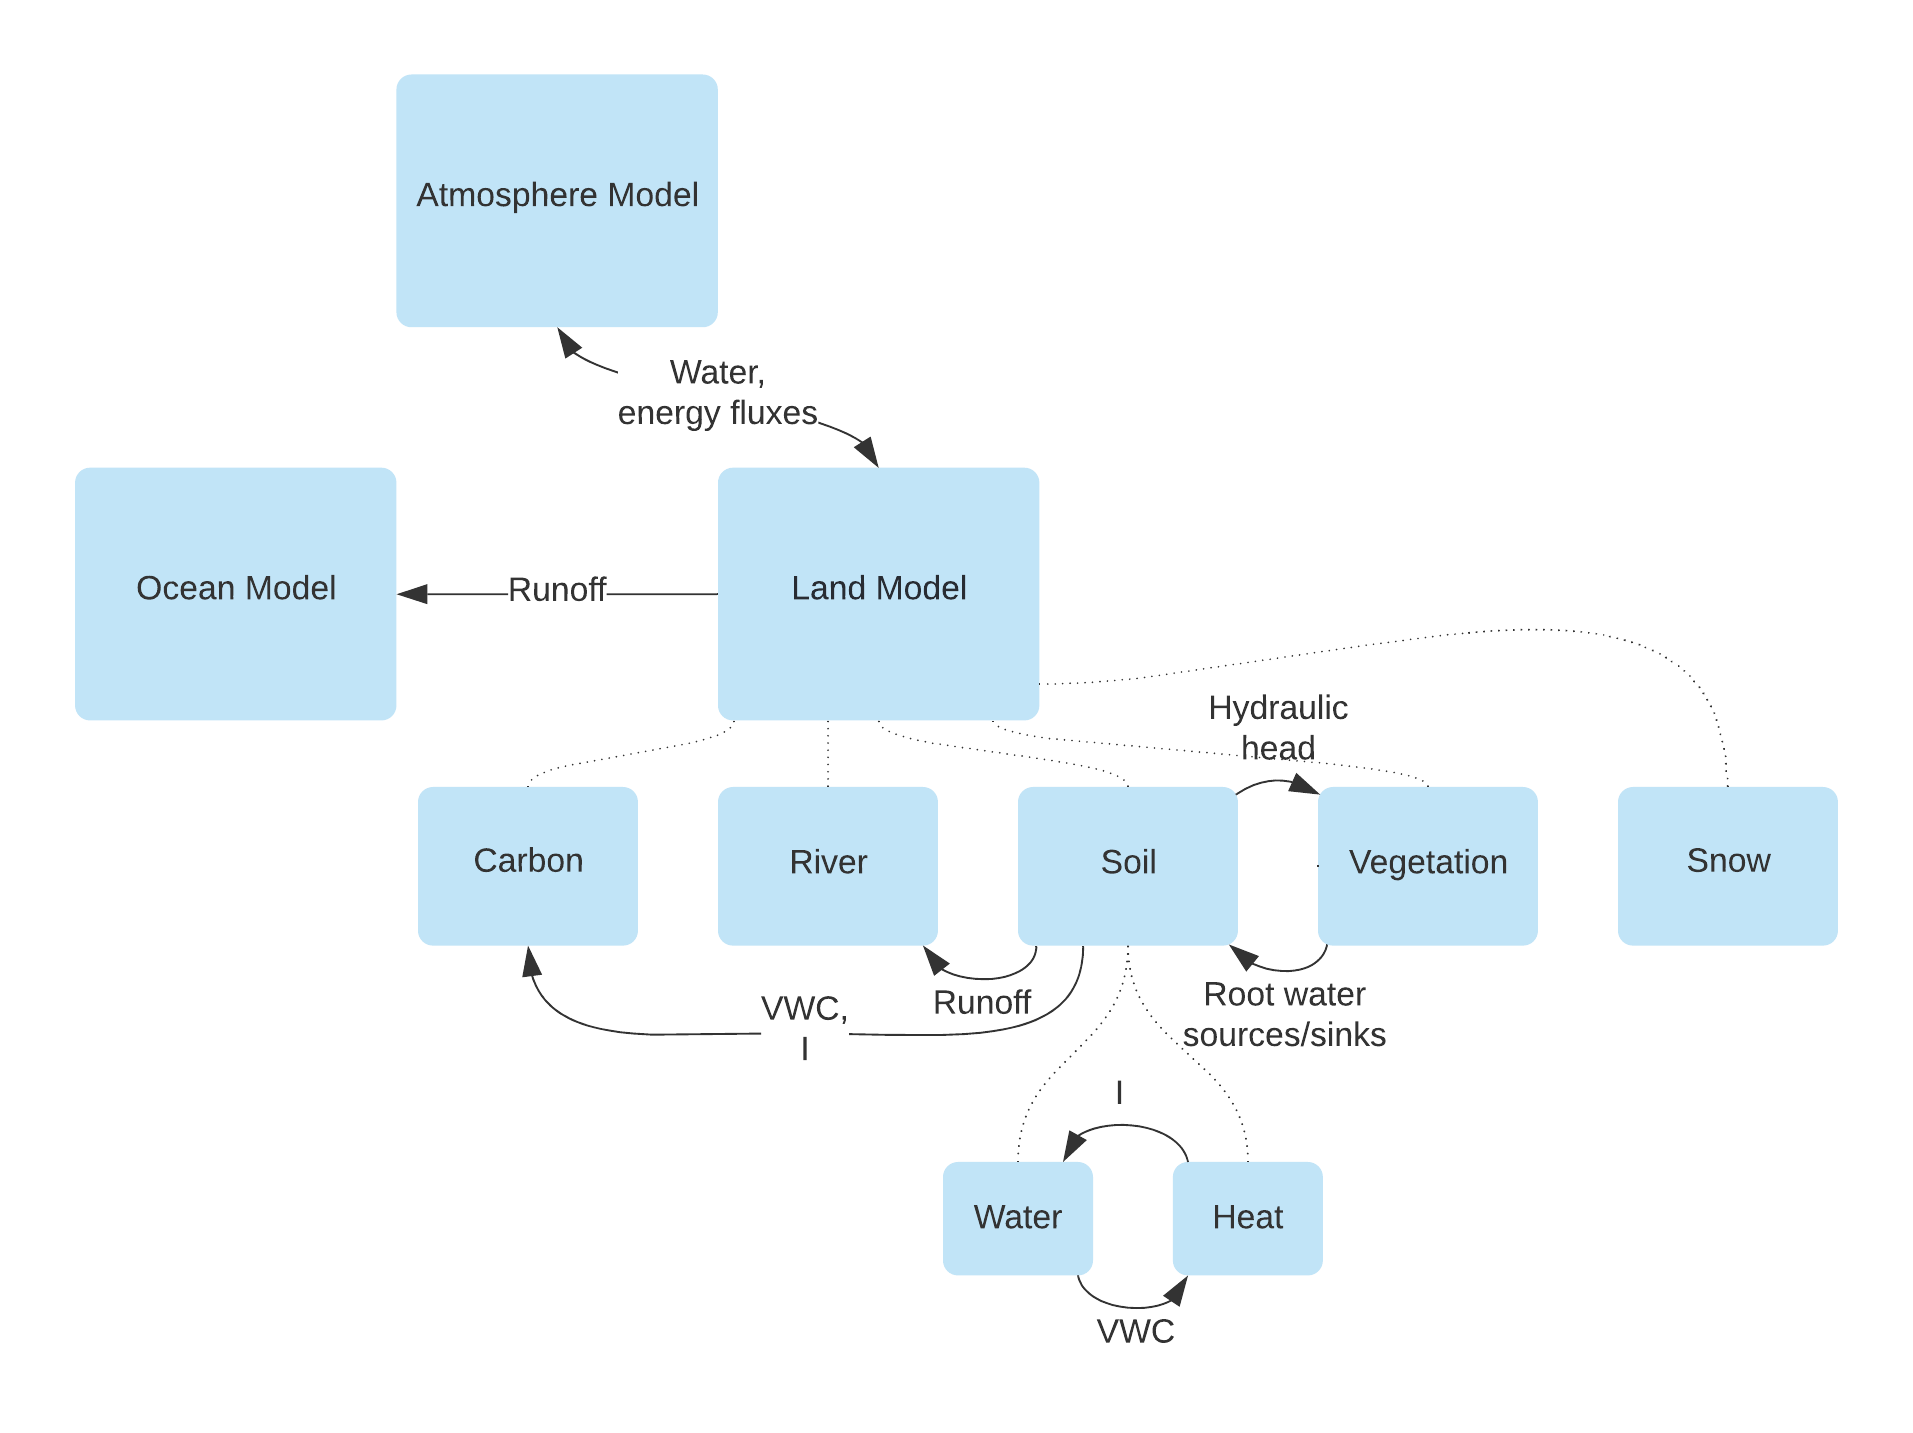
\includegraphics[width=10cm,height=10cm,keepaspectratio]{CLIMA-land/LM_figures/JPLCLIMA_LM_DESIGN_20200915.png}
\caption{Schematic of land model components and their interactions. For example, the canopy model interacts with the soil model through source/sink terms representing processes such as water uptake by roots, and it interacts with turbulent fluxes in the atmospheric near-surface layer through exchange of momentum, energy, and water. \hl{Hrishi:[The flux going from the Land Model to Ocean Model would be 'discharge', not 'runoff'. If we are implementing River Model as a separate model, then the flux would go from River Model directly to the Ocean Model (instead of from the Land Model).]}}
\label{f:land_model_schematic}
\end{figure}
% Please add the following required packages to your document preamble:
% \usepackage{graphicx}
\begin{table}[]
\resizebox{\textwidth}{!}{%
\begin{tabular}{|l|l|l|l|}
\hline
Module [code]         & Input requirements [From]                                                                & Output requirements                                                       & Module requirements                      \\ \hline
Carbon [C]            & \begin{tabular}[c]{@{}l@{}}GPP [F], \\ Soil water profile [W], \\ Soil temperature profile [E]\end{tabular}                                                               & \begin{tabular}[c]{@{}l@{}}Carbon states\\ (Biomass, inc. foliar, roots, wood;\\ Dead organic C) \\ Carbon fluxes \\ (respiration, disturbance fluxes)\end{tabular} & \begin{tabular}[c]{@{}l@{}}The carbon module will calculate \\ internal land biosphere carbon transfers \\ (allocation, mortality, mineralization), \\ and gross land-atmosphere C fluxes \\ (respiration, fires)\end{tabular} \\ \hline

Structure [S]         & Biomass [C]                                                             & \begin{tabular}[c]{@{}l@{}}Biophysical states:\\ Canopy height, Chlorophyll, \\Root profile, LMA\end{tabular}                                                        &                                                                   \\ \hline
Soil water [H]        & \begin{tabular}[c]{@{}l@{}}Soil freeze/thaw state [E] \\ Precipitation [A]\\ Evaporation [F], \\ Transpiration (vertically resolved), \\ root profile [S]\end{tabular} &
\begin{tabular}[c]{@{}l@{}}
Vertical soil water states\\Soil water fluxes\\Runoff\end{tabular}                                                                                                                  & \begin{tabular}[c]{@{}l@{}}Module will calculate vertical \\ water flow in soil Darcy’s law, \\ Richards' equations, hydraulic \\redistribution,  runoff, etc.\end{tabular}                                                     \\ \hline
Soil heat storage [E] & Soil water [H], Precip. temp [A]
& 
\begin{tabular}[c]{@{}l@{}}
Vertical temperature profile\\
Runoff temperature       \end{tabular}                                               &                                                                                                \\ \hline
%%%%%%(SPAC-Flux)%%%%%
\begin{tabular}[c]{@{}l@{}}
Land-to-atmosphere\\ fluxes [F]  \\
(previously SPAC-Flux)
\end{tabular}

        & \begin{tabular}[c]{@{}l@{}}Atmospheric variables [A], \\ Biophysical states[S], \\ Soil water profile [H], \\ Soil energy profile [E],\end{tabular}                   & \begin{tabular}[c]{@{}l@{}}Land-surface Fluxes\\ GPP, evapotranspiration, H, $\lambda$E, radiative fluxes \end{tabular}                                 & 

\begin{tabular}[c]{@{}l@{}} Canopy P interception\\ Radiative transfer in canopy     \end{tabular}                                                        \\ \hline

River routing [R]        & \begin{tabular}[c]{@{}l@{}} Soil runoff [H] \end{tabular}                             & \begin{tabular}[c]{@{}l@{}} River Discharge\end{tabular}                                             &                                     \\ \hline \hline \hline


CliMA Atmosphere [A]        & \begin{tabular}[c]{@{}l@{}}Land surface fluxes [F], \\ Land biosphere fluxes [C]\end{tabular}                             & \begin{tabular}[c]{@{}l@{}}Atmospheric variables [for land]\\ Radiative fluxes, precipitation, temperature, humidity,\end{tabular}                                             &                                     \\ \hline

CliMA Ocean [O]        & \begin{tabular}[c]{@{}l@{}}River discharge [R] \end{tabular}                             & \begin{tabular}[c]{@{}l@{}} Ocean variables (for land) Sea Level\end{tabular}                                             &                                     \\ \hline
\end{tabular}}
\caption{\label{tab:LM-modules}Overview of inputs, outputs, and functional requirements of land model components.}
\end{table}

Chapter~\ref{c:soil} begins with a description of the soil model and its treatment of the energy and water balance of soil, including boundary conditions covering how soil interacts with the atmosphere. \hl{[add rest of overview]}.

\section{Goals}

\begin{itemize}
    \item Provide a complete and self-contained documentation of the scientific concepts underlying the land model.
    \item Establish a consistent notation for the governing equations, which may guide data structures and variable names in the code.
    \item Establish a consistent set of approximations for the governing equations that allow the land model to be used both on climate model scales (tens of kilometers and larger) and large-eddy simulation (LES) scales (kilometers and smaller).
    \item Describe boundary conditions that ensure conservation of energy, water, and tracer (e.g., carbon) masses during exchanges with other climate model components, while treating the interfacial layer (e.g., near-surface turbulence in the atmosphere) consistently across model components.
    \item Harmonize equations and boundary conditions to facilitate coupling with the \href{https://github.com/climate-machine/Design-Docs/blob/master/CLIMA-atmos/}{CLIMA atmosphere} model.
    \item Lay out the concepts in a way that can be directly translated into code. Key equations that appear in the code are highlighted in \hlpaleblue{blue boxes}.
    \item Document benchmark cases for testing the land model.
\end{itemize}

\section{Non-Goals}

\begin{itemize}
    \item Discuss software architecture and data structures.
    \item Discuss generic aspects of numerical methods (but we will discuss a few land model-specific aspects).
    \item Discuss implementation details such as variable names and computational aspects.
\end{itemize}
Details of numerical methods are covered in a \href{https://github.com/climate-machine/Design-Docs/tree/master/CLIMA-numerics}{separate design document}.

\chapter{Soil Physics}\label{c:soil}

The soil model represents the transport of energy and moisture in soil, links them to atmospheric boundary conditions above, and provides water input for runoff models (e.g., along the surface or in rivers). Vegetation is linked to the soil model through root extraction, which represents water sources and sinks in soil, and through modulation of radiation reaching the top of the soil.  This chapter describes the energy and water balances in soil and how atmospheric boundary conditions and vegetation link to them.

\hl{[synopsis of what's new. Soil model achieves a number of goals outlined by]} \citep{Clark15a}

\section{Composition of Soil}

\subsection{Bulk Soil}

We take soil to consist of a dry soil matrix (composed of sand, clay, rock, etc.) with pore spaces that may contain liquid water, ice, and gases (air with water vapor). The bulk density of the soil mixture, including water, is $\rho$ ($\mathrm{kg~m^{-3}}$). The composition of soil is characterized by mass fractions (mass of constituent divided by total mass of soil), which each depend on a space coordinate and time:
\begin{itemize}
    \item $q_{ds}$: mass fraction of dry soil,
    \item $q_l$: mass fraction of liquid water,
    \item $q_i$: mass fraction of ice,
    \item $q_w = q_l + q_i$: mass fraction of total water (liquid and ice).
\end{itemize}
We neglect the small mass (but not the volume) of gases in pore spaces, so that this enumerates all constituents of soil that contribute to soil mass; therefore, 
\[
q_{ds} + q_l + q_i = q_{ds} + q_w = 1.
\]

Because the primary constituents of soil are essentially incompressible, the composition of soil is commonly expressed in terms of volume fractions (e.g., volume of liquid water per volume of soil). The volume fractions $\theta_{\cdot}$ of the constituents are related to the mass fractions $q_{\cdot}$ through
\begin{subequations}\label{e:vol_fractions}
\begin{align}
    \theta_{ds} &= \frac{q_{ds} \rho}{\rho_{ds}} \\
    \theta_l &= \frac{q_l \rho}{\rho_l}, \\
    \theta_i &= \frac{q_i \rho}{\rho_i}, \\
    \theta_w &= \theta_l + \theta_i.
\end{align}
\end{subequations}
Here, $\rho_{ds}$ is the particle density of dry soil (i.e., the density of the soil particles alone, without pore spaces), and $\rho_l$ and $\rho_i$ are the densities of liquid water and ice, respectively. We take liquid water to be incompressible, and the densities $\rho_l$ of liquid and $\rho_i$ of ice to be constant. The density variations of liquid water are of order $10^{-3}$ over typical soil temperatures, which is negligible compared with other variations, for example, of the viscosity of liquid water. We summarize the water content of soil by the  tuple $\vec{\theta} = (\theta_l, \theta_i)$.

While the mass fractions of dry soil and water sum to one, the volume fractions do not: Gases, which are assumed to have zero mass, occupy a volume fraction $\theta_g = 1 - (\theta_{ds} + \theta_w)$. Gases, liquid water, and ice occupy pore spaces in the soil matrix. The volume fraction of pore spaces that can be filled with either gas or water is the porosity 
\begin{equation}\label{e:porosity}
    \nu_p = \theta_g + \theta_w =  1 - \theta_{ds}.
\end{equation}
The porosity is the volume fraction filled with gas when the soil is dry ($\theta_w=0$), or it is the volume fraction occupied by liquid water when all voids are filled with liquid water ($\theta_g = \theta_i = 0$). 

\subsection{Dry Soil}

The dry soil portion of the bulk soil in turn consists of constituents such as mineral soil, gravel, organic matter, or bedrock, which all have different thermodynamic and hydraulic properties.  Let $\nu_{i}$ indicate the dry volume fraction of constituent $\chi_i$ in the total volume of soil, with $\chi_i$ labeling the constituents, for example,
\[
\chi_i \in \{ {\mathrm{sand}}, {\mathrm{clay}}, {\mathrm{silt}}, {\mathrm{gravel}}, \mathrm{organic~matter}, {\mathrm{bedrock}} \}.
\]
We include bedrock in the soil constituents to be able to directly apply our soil model in bedrock, simply by modifying location-specific (3D) thermodynamic and hydraulic parameters. If the $\nu_i$'s enumerate all constituents of dry soil, the volume fractions sum to the total dry-soil volume fraction $1-\nu_p$,
\[
\sum_i \nu_{i} = 1-\nu_p.
\] 
We use the tuple $\vec{\nu} = (\nu_p, \nu_i)$ to summarize the composition of dry soil, including its porosity $\nu_p$. The dry soil composition depends on a space coordinate, and it may also vary on long (decadal and longer) timescales.

\subsection{Soil Density}

The particle density of dry soil is the weighted mean of the dry particle densities $\rho_{\chi_i}$ of the constituents $\chi_i$:
\begin{equation}\label{d:dry_soil_density}
    \rho_{ds}(\vec{\nu})  = (1-\nu_p)^{-1} \sum_i \nu_{i} {\rho}_{\chi_i}.
\end{equation}
This gives the bulk soil density, including the water contained in the soil,  
\begin{equation}\label{e:bulk_density}
\rho (\vec{\theta}; \vec{\nu}) = (1-\nu_p) \rho_{ds} + \theta_l \rho_l + \theta_i \rho_i,
\end{equation}
which follows from the definition of the volume fractions \eqref{e:vol_fractions} and of porosity \eqref{e:porosity}. 

\section{Heat Capacity of Soil}

\subsection{General Formulation}

The specific heat capacity of soil (heat capacity per unit mass, $\mathrm{J~kg^{-1}~K^{-1}}$) is the mass-weighted sum of the specific heat capacities of the constituents
\begin{equation}\label{e:soil_specific_heat}
    c_s = (1-q_w) c_{ds} + q_l c_{l} + q_i c_{i},
\end{equation}
where we have used $q_{ds} = 1 - q_w$, and the specific heat capacities of the constituents are:
\begin{itemize}
    \item $c_{ds}$: Specific heat capacity of dry soil,
    \item $c_l$: Specific heat capacity of liquid water,
    \item $c_i$: Specific heat capacity of ice.
\end{itemize}
Consistent with neglecting the mass of the gas constituents, we neglect their contribution to the soil specific heat capacity.

The specific heat capacity of dry soil depends on spatially varying soil properties (discussed below). We take the specific heat capacities of liquid water and ice to be constants, consistent with the thermodynamics of the  \href{https://github.com/climate-machine/Design-Docs/blob/master/CLIMA-atmos/}{CLIMA atmosphere} model. These constants should be chosen to be the same in atmosphere, ocean, land, and other models; they are set in the \href{https://github.com/CliMA/CLIMAParameters.jl}{CLIMAParameters} module.

Because, as is common, we use volume fractions to characterize the composition of the soil, we also use the volumetric heat capacities (heat capacities per unit volume, $\mathrm{J~m^{-3}~K^{-1}}$):
\begin{subequations}\label{e:vol_heat_capacities}
\begin{align}
    \tilde{c}_{ds} &= \rho_{ds} c_{ds},\\
    \tilde{c}_{l} &= \rho_{l} c_{l},\\
    \tilde{c}_{i} &= \rho_{i} c_{i}.
\end{align}
\end{subequations}
In terms of volume fractions of constituents, the combined volumetric heat capacity of soil is the weighted mean
\begin{equation}\label{e:soil_spec_heat_volume_0}
    \tilde c_s = \rho c_s = (1-\nu_p) \tilde c_{ds} + \theta_l \tilde c_l + \theta_i \tilde c_i.
\end{equation}
This expression for the volumetric heat capacity follows by substituting the definitions of volume fractions \eqref{e:vol_fractions}, porosity \eqref{e:porosity}, and volumetric heat capacities \eqref{e:vol_heat_capacities} into the definition of the specific heat capacity of soil \eqref{e:soil_specific_heat}. Instead of referring the heat capacity of dry soil to a unit volume of solid soil only (excluding the pore space volume), it is convenient to use a bulk heat capacity of a volume of dry soil that includes the pore space volume:
\begin{equation}\label{e:bulk_dry_heat_capacity0}
    \check{c}_{ds}(\vec{\nu}) = (1-\nu_p) \tilde{c}_{ds}.
\end{equation}
In terms of this bulk volumetric heat capacity of dry soil, the volumetric heat capacity of soil \eqref{e:soil_spec_heat_volume_0} becomes
\begin{empheq}[box=\eqnbox]{equation}\label{e:soil_spec_heat_volume}
    \tilde c_s (\vec{\theta}; \vec{\nu}) = \check c_{ds}(\vec{\nu}) + \theta_l \tilde c_l + \theta_i \tilde c_i,
\end{empheq}
which is a function of the soil composition: it depends on water content  $\vec{\theta}$ (a model state variable) and parametrically on the dry-soil composition $\vec{\nu}$. The expression \eqref{e:soil_spec_heat_volume} makes it clear that the heat capacity of soil increases when pore spaces are filled with soil water. (Here and throughout this document, we use tilde and check accents to indicate thermodynamic quantities referenced to volume rather than mass.) 

\subsection{Heat Capacity of Dry Soil}

The volumetric heat capacity of dry soil is commonly approximated as the weighted mean of the volumetric heat capacities of mineral soil, gravel, organic matter, bedrock, and possibly other constituents \citep{Farouki81a}. If ${\tilde c}_{\chi_i}$ denotes the volumetric heat capacity of constituent $\chi_i$, the volumetric heat capacity of dry soil is the weighted mean 
\begin{equation}\label{e:dry_soil_heat_capacity}
\tilde{c}_{ds} (\vec{\nu}) = (1-\nu_p)^{-1} \sum_i \nu_{i} {\tilde c}_{\chi_i}.
\end{equation}
This is the volumetric heat capacity of the solid components of dry soil only, that is, excluding the pore space volume. The bulk heat capacity of a volume of dry soil that includes the pore space volume is
\begin{equation}\label{e:bulk_dry_heat_capacity}
    \check{c}_{ds} (\vec{\nu})  = (1-\nu_p) \tilde{c}_{ds} = \sum_i \nu_{i} {\tilde c}_{\chi_i}.
\end{equation}
This bulk dry heat capacity is commonly tabulated. 

Sources of the data needed to specify soil composition $\vec{\nu}$ and heat capacities $\check c_{ds}$ are listed in section~\ref{s:soil_data}.

\section{Thermodynamic State of Soil}

\subsection{Internal Energy}

We characterize the thermodynamic state of soil by its internal energy. The specific internal energy (energy per unit mass, $\mathrm{J~kg^{-1}}$) is the mass-weighted mean of the constituent specific internal energies of dry soil $I_{ds}$, liquid water $I_l$, and ice $I_i$,
\begin{equation}\label{e:energy_soil}
    I = (1-q_w) I_{ds} + q_l I_l + q_i I_i.
\end{equation}
Gases are again neglected, consistent with neglecting their mass. The specific internal energies of the constituents depend on the temperature $T$ of the constituents (which are assumed to be in local thermal equilibrium, so they have the same temperature in any one location) and the specific heat capacities:
\begin{subequations}\label{e:soil_internal_energies}
\begin{align}
I_{ds}(T; \vec{\nu}) & = c_{ds}(\vec{\nu}) (T - T_0),  \\
I_l(T) & = c_{l} (T - T_0), \\
I_i(T) & = c_{i} (T - T_0) - I_{i,0}.
\end{align}
\end{subequations}
The temperature $T_0$ is a reference temperature at which the specific internal energy of soil and liquid water are taken to vanish, and $I_{i,0}$ is the difference in specific internal energy between ice and liquid water at $T_0$. As is common for condensed phases (liquids and solids), we equate the internal energies and enthalpies of liquid water and ice, and approximate the specific internal energy difference $I_{i,0}$ by the specific enthalpy difference at $T_0$, which is the specific latent heat of fusion $L_{f,0}$ at $T_0$: 
\begin{equation}
    I_{i,0} = L_{f,0}.
\end{equation} 
These definitions for the internal energy of soil are consistent with those for the \href{https://github.com/climate-machine/Design-Docs/blob/master/CLIMA-atmos/}{CLIMA atmosphere} model. The reference temperature $T_0$ is arbitrary, but the specific latent heat of fusion $L_{f,0}$ must be chosen as that at $T_0$. The thermodynamic properties of water must be chosen to be the same for soil, atmosphere, and other model component, to ensure thermodynamic consistency. 

For the soil model, it is again convenient to use internal energies per unit volume ($\mathrm{J~m^{-3}}$) rather than the internal energies per unit mass. The internal energies per unit volume are related to the specific internal energies by
\begin{subequations}
\begin{align}
    \tilde I_{ds} &= \rho_{ds} I_{ds},\\
    \tilde I_{l}  &= \rho_{l} I_{l},\\
    \tilde I_{i}  &= \rho_{i} I_{i}.
\end{align}
\end{subequations}
Using the fact that the specific heat capacity of soil \eqref{e:soil_specific_heat} is the weighted mean of those of the constituents, together with the relation \eqref{e:soil_spec_heat_volume} for the volumetric specific heat, and the definition \eqref{e:vol_fractions} of the volume fractions, the total internal energy per unit volume can be written as
\begin{empheq}[box=\eqnbox]{equation}\label{e:vol_internal_energy}
\begin{split}
    \tilde I(T, \vec{\theta}; \vec{\nu})  &= \rho I 
    = \theta_{ds} \tilde I_{ds}(T; \vec{\nu}) + \theta_l  \tilde I_l(T) + \theta_i  \tilde I_i(T)\\
    &= \tilde{c}_s(\vec{\theta}; \vec{\nu}) (T - T_0) - \theta_i \rho_i L_{f,0}.
\end{split}
\end{empheq}
The internal energy $\tilde I$ of soil depends on temperature $T$ and, through the volumetric specific heat $\tilde c_s(\vec{\theta}; \vec{\nu})$, on water content $\vec{\theta}$ and dry-soil composition $\vec{\nu}$, the latter being a location-dependent parameter (section~\ref{s:soil_data}).

\subsection{Temperature}

Given the internal energy $\tilde I$ and composition ($\vec{\theta}; \vec{\nu}$) of the soil, the definition \eqref{e:vol_internal_energy} can be inverted to give the soil temperature
\begin{empheq}[box=\eqnbox]{equation}%\begin{equation}
\label{e:temperature_from_I}
    T = T_0 + \frac{\tilde{I} + \theta_i \rho_i L_{f,0}}{\tilde{c}_s(\vec{\theta}; \vec{\nu})}.
%\end{equation}
\end{empheq}
Thus, we can use the internal energy $\tilde I$ as a prognostic variable in a soil model and obtain the temperature $T$ from that and from knowledge of the composition ($\vec{\theta}; \vec{\nu}$) of the soil. If only the total water volume fraction $\theta_w$ is used as a prognostic variable, we can solve for temperature $T$ and the phase partitioning of $\theta_w$ into $\theta_l$ and $\theta_i$ simultaneously, by assuming that all water above the freezing temperature is liquid, and all water below the freezing temperature is ice, with an internal-energy dependent partitioning between liquid and ice at the freezing temperature \citep{Longo19a}. However, our hydrologic model predicts $\theta_l$ and $\theta_i$ separately (section~\ref{s:water_balance}), to be able to represent soils that, when the resolved-scale temperature is around freezing, are partially frozen and unfrozen on subgrid scales. In that case, with $\theta_l$ and $\theta_i$ available separately, the relation \eqref{e:temperature_from_I} can be used to directly infer temperature given internal energy.
 
Using internal energy rather than temperature as a prognostic variable is advantageous because internal energy, unlike temperature, is conserved when water freezes or thaws. Thus, internal energy is unaffected by phase transitions of water and remains continuous at freezing/thawing fronts.

\section{Energy Balance}

\subsection{Conservation Law}

The conservation law for internal energy is \citep[cf.][]{Walko00a,Longo19a}
\begin{empheq}[box=\eqnbox]{equation}%\begin{equation}
\label{e:energy_conservation}
    \frac{\partial \tilde I}{\partial t} =  - \divergence \bigl(\vec{\tilde J} + \vec{\tilde D}\bigr) - \tilde I_l(\tilde R_l + \tilde R_r) + \tilde Q - \divergence \vec{\tilde F}_R.
\end{empheq}
On the right-hand sides are the divergences of fluxes and source/sink terms, which lead to changes of internal energy:
\begin{itemize}
    \item Conductive heat fluxes $\vec{\tilde J}$ ($\mathrm{W~m^{-2}}$);
    \item Energy fluxes $\vec{\tilde D}$ ($\mathrm{W~m^{-2}}$) carried by moving (diffusing) water. 
    \item Internal energy carried off by subsurface runoff $\tilde R_l$ and other sinks of water $\tilde R_r$ ($\mathrm{s^{-1}}$), e.g., owing to root extraction;
    \item External heat sources/sinks $\tilde Q$ ($\mathrm{W~m^{-3}}$), such as metabolic heat from soil microbes;
    \item Any radiative energy fluxes $\vec{\tilde F}_R$ ($\mathrm{W~m^{-2}}$) that penetrate into the soil. (Radiative fluxes penetrating into the soil are generally not resolved in soil models and only enter as upper boundary conditions (section~\ref{s:soil_boundary_conditions}), so that their flux divergence in the soil vanishes.\footnote{The radiative energy flux also appears in the \protect\href{https://github.com/climate-machine/Design-Docs/blob/master/CLIMA-atmos/}{CLIMA atmosphere} model, where it is referenced to unit mass, $\vec{F}_R$ ($\mathrm{W~m~kg^{-1}}$), with $\vec{\tilde F}_R = \rho \vec{F}_R$.}) 
\end{itemize}

Because vertical variations in soil generally are much greater than horizontal variations, the derivative operator in all current Earth system models is approximated by its vertical component ($\nabla \approx \partial/\partial z$), reducing the conservation law \eqref{e:energy_conservation} to a one-dimensional partial differential equation. However, in what follows we keep the notation general, to develop the model setup to be generally usable in 3D as well as 1D. 

The conductive heat flux is given by Fourier's law as
\begin{empheq}[box=\eqnbox]{equation}
%\begin{equation}
    \vec{\tilde J} = - \kappa \grad T, 
\end{empheq}
where $\kappa = \kappa(\vec{\theta}; \vec{\nu})$ ($\mathrm{W~m^{-1}~K^{-1}}$) is the thermal conductivity of soil, which we take to be isotropic (scalar) and which depends on the soil composition $(\vec{\theta}; \vec{\nu})$. The energy flux carried by diffusion of water is 
\begin{empheq}[box=\eqnbox]{equation}
    \vec{\tilde D} = \tilde I_l \vec{\tilde d}_{l},
\end{empheq}
where the diffusive flux of liquid water $\vec{\tilde d}_{l}$ is discussed further in section~\ref{s:water_balance}. 

The conservation law \eqref{e:energy_conservation} for internal energy in soil is approximately the conservation law for total energy. Kinetic energy and gravitational potential energy in principle also contribute to the total energy. But the kinetic energy of water motion is orders of magnitude smaller than the internal energy. And conversion of gravitational potential energy associated with water motion into internal energy likewise is negligible. Hence, the internal energy conservation law closely approximates the total energy conservation law. 

Table~\ref{t:thermodynamics_soil} summarizes the thermodynamic quantities entering the energy balance of soil.
\begin{table}[]
\resizebox{\textwidth}{!}{%
\begin{tabular}{lllll}
State Variables         & Description                           & Units                     & Definition                            & Typical Value     \\ \hline
$\tilde{I}$             & Internal energy per unit volume       & $\mathrm{J~m^{-3}}$       & Eq.~\eqref{e:vol_internal_energy}     & $4 \times 10^6~\mathrm{J~m^{-3}}$   \\
$\theta_l$, $\theta_i$  & Volume fractions of liquid/ice        &   $\mathrm{m^3~m^{-3}}$   & Eq.~\eqref{e:vol_fractions}           & $0 \le (\theta_l, \theta_i) \le \nu_p$ \\
$\vec{\theta} = (\theta_l, \theta_i)$ & Water content of soil                 &                           &                                       &               \\[2ex]
%\hline
Functions of State      & Description                           & Units                     & Definition                            & Typical Value \\ \hline
$\theta_w = \theta_l + \theta_i$ & Volume fraction of total water & $\mathrm{m^3~m^{-3}}$   & Eq.~\eqref{e:vol_fractions}           &    $0 \le \theta_w \le \nu_p$  \\
$T$                     & Soil Temperature                      & K                         & Eq.~\eqref{e:temperature_from_I}      & 288 K         \\
$\rho$                  & Bulk density of soil                  & $\mathrm{kg~m^{-3}}$      & Eq.~\eqref{e:bulk_density}            & $1.5\times 10^3~\mathrm{kg~m^{-3}}$ \\
$\tilde c_s$            & Volumetric heat capacity              & $\mathrm{J~m^{-3}~K^{-1}}$& Eq.~\eqref{e:soil_spec_heat_volume}   & $2\times 10^{6}~\mathrm{J~m^{-3}~K^{-1}}$ \\
$\kappa$              & Thermal conductivity                    & $\mathrm{W~m^{-1}~K^{-1}}$& Eq.~\eqref{e:soil_conductivity}       & $0.85~\mathrm{W~m^{-1}~K^{-1}}$ \\
$\kappa_{\mathrm{sat}}$ & Saturated thermal conductivity        & $\mathrm{W~m^{-1}~K^{-1}}$& Eq.~\eqref{e:saturated_theral_conductivity}  & $3~\mathrm{W~m^{-1}~K^{-1}}$ \\
$K_e$                   & Kersten number                        &                           & Eq.~\eqref{e:Kersten}   & $0 \le K_e \le 1$ \\[2ex]
%\hline
Global Constants        & Description                           & Units                     &                                       & Value \\ \hline
$T_0$                   & Reference temperature                 & K                         &                                       & $273.16~\mathrm{K}$ \\
$L_{f,0}$               & Latent heat of fusion at $T_0$        & $\mathrm{J~kg^{-1}}$      &                                       & $333.6 \times 10^3~\mathrm{J~kg^{-1}}$\\
$\tilde c_l$            & Volum.\ heat capacity liquid water    & $\mathrm{J~m^{-3}~K^{-1}}$&                                       & $4.18 \times 10^6~\mathrm{J~m^{-3}~K^{-1}}$ \\
$\tilde c_i$            & Volumetric heat capacity ice          & $\mathrm{J~m^{-3}~K^{-1}}$&                                       & $1.93 \times 10^6~\mathrm{J~m^{-3}~K^{-1}}$ \\[2ex]
Empirical Properties    & Description                           & Units                     & Obtained from                         & Typical Value \\ \hline
$\nu_p$                 & Porosity                              &                           & Input data                            & $0\le \nu_p \le 1$ \\
$\nu_i$                 & Volume fraction of $\chi_i$           &                           & Input data                            & $0\le \chi_i \le 1$     \\
$\vec{\nu} = (\nu_p, \nu_i)$ & Composition of dry soil               &                           & Input data                            &                       \\
$\tilde c_i$            & Volumetric heat capacity $\chi_i$     &                           & Input data                            &       \\
$\check c_{ds}$         & Bulk vol.\ heat capacity dry soil     & $\mathrm{J~m^{-3}~K^{-1}}$& Eq.~\eqref{e:bulk_dry_heat_capacity}  & $1 \times 10^6~\mathrm{J~m^{-3}~K^{-1}}$ \\
$\rho_{ds}$             & Particle density dry soil             & $\mathrm{kg~m^{-3}}$      & Eq.~\eqref{d:dry_soil_density}        & $2 \times 10^3~\mathrm{kg~m^{-3}}$ \\
$\kappa_{\mathrm{dry}}$ & Dry thermal conductivity              & $\mathrm{W~m^{-1}~K^{-1}}$& Input data                            & $1.5~\mathrm{W~m^{-1}~K^{-1}}$ 
%\hline
\end{tabular}%
}% end resizebox
\caption{\label{t:thermodynamics_soil}Key thermodynamic variables and parameters in soil model.}
\end{table}

\subsection{Empirical Relations for Thermal Conductivity of Soil}

To close the energy balance, it remains to specify the thermal conductivity $\kappa(\vec{\theta}; \vec{\nu})$ of soil. The thermal conductivity of soil varies depending on mineral composition, organic matter content, porosity, and the water content of soils. The overall thermal conductivity of soil is an average of the conductivity of its constituents. For example, quartz has a thermal conductivity three times greater than clay minerals, so soils such as sands with high quartz content have a greater thermal conductivity than do clay soils. Organic material has an extremely low thermal conductivity, and peat soils with high organic matter content have a thermal conductivity that is one-quarter to one-third of that of mineral soils. The thermal conductivity of water is more than 20 times that of air, so the thermal conductivity of soil increases as soil moisture increases and fills pore spaces otherwise occupied by air. Additionally, the thermal conductivity of frozen soil is larger than that of unfrozen soil with the same total water content because ice conducts heat more efficiently than liquid water. 

We model the thermal conductivity, as is common, as a weighted mean of the conductivities of dry soil $\kappa_{\mathrm{dry}}$ and water saturated soil $\kappa_{\mathrm{sat}}$,
\begin{empheq}[box=\eqnbox]{equation}
\label{e:soil_conductivity}
\kappa = K_e \kappa_{\mathrm{sat}} + (1-K_e) \kappa_{\mathrm{dry}}.
\end{empheq}
The weighting factor is the dimensionless Kersten number $K_e = K_e(\vec{\theta})$ ($0 \le K_e \le 1$), an empirical function that monotonically increase with soil moisture content \citep{Farouki81a,Dai19a}. 

The thermal conductivities of dry soil $\kappa_{\mathrm{dry}} = \kappa_{\mathrm{dry}}(\vec{\nu})$ and saturated soil $\kappa_{\mathrm{sat}} = \kappa_{\mathrm{sat}}(\vec{\theta}; \vec{\nu})$ are weighted averages of the conductivities of the soil constituents, with arithmetic, geometric, and harmonic means being used in different models \citep{Dai19a}: 
\begin{itemize}
    \item The arithmetic mean is adequate for a soil matrix that is macroscopically homogeneous and isotropic at the resolution of the model, which is a good approximation at high (centimeter-scale) resolution. 
    \item The harmonic mean,
    \[
    \kappa = \left( \frac{1}{N} \sum_i^N \frac{1}{\kappa_i} \right)^{-1},
    \]
    with constituent conductivities $\kappa_i$, is appropriate if the constituents of soil are layered on scales below the model resolution, and one considers thermal conduction through a stack of such layers, viewed as a series of resistors to thermal conduction. The harmonic mean is dominated by the smallest conductivity $\kappa_i$ and vanishes if any conductivity $\kappa_i$ is zero. This may be a good approximation at lower resolution when soils are in fact layered and the focus is on vertical thermal conduction. 
    \item The geometric mean 
    \[
    \kappa = \left( \prod_i^N \kappa_i \right)^{1/N},
    \]
    lies in between the arithmetic and harmonic mean (by the Arithmetic Mean-Geometric Mean-Harmonic Mean Inequality). It is a compromise between arithmetic and harmonic means. 
\end{itemize}
Hence, the appropriate form of averaging or homogenization is resolution dependent. No general theoretical framework appears to exist that guides under which circumstances which kind of mean is to be used; various types of means are used in existing soil models without clear reference to resolution and soil heterogeneity. 

\subsubsection{Dry Thermal Conductivity}

For now, we use global data that estimate the dry thermal conductivity $\kappa_{\mathrm{dry}}(\vec{\nu})$ on the basis of soil composition data and conductivity models \citep{Dai19a} (section~\ref{s:soil_data}). 

\subsubsection{Saturated Thermal Conductivity}

The thermal conductivity $\kappa_{\mathrm{sat}}(\vec{\theta}; \vec{\nu})$ of saturated soils depends on whether the soil is frozen or not, with an unfrozen saturated thermal conductivity $\kappa_{\mathrm{sat, unfrozen}}(\vec{\nu})$ and a frozen saturated thermal conductivity  $\kappa_{\mathrm{sat, frozen}}(\vec{\nu})$. To be consistent with how these saturated thermal conductivities are commonly estimated via geometric means \citep[e.g.,][]{Balland05a}, we use the geometric-mean saturated thermal conductivity
\begin{empheq}[box=\eqnbox]{equation}\label{e:saturated_theral_conductivity}
    \kappa_{\mathrm{sat}}(\vec{\theta}; \vec{\nu}) = \left[\kappa_{\mathrm{sat, unfrozen}}(\vec{\nu})\right]^{\theta_l/\theta_w}
    \left[\kappa_{\mathrm{sat, frozen}}(\vec{\nu})\right]^{\theta_i/\theta_w},
\end{empheq}
where $\theta_w=\theta_l + \theta_i$. We use global tabulated estimates of $\kappa_{\mathrm{sat, unfrozen}}$ and $\kappa_{\mathrm{sat, frozen}}$ \citep{Dai19a} (section~\ref{s:soil_data}). Note that in the expressions for the saturated thermal conductivity and the thermal conductivity of the solids in \citet{Dai19a} and \citet{Balland05a}, there appear the volume fractions of soil solids relative to the soil (including pore space), which we denote $\nu_{i}$, with $\sum_i \nu_i = 1-\nu_p$, and the volume fractions relative to soil solids only, which we denote $\hat\nu_{i}$, with $\sum_i \hat\nu_i = 1$.

\subsubsection{Kersten Number}

\citet{Dai19a} compared various empirical formulations for the Kersten number (along with ways of estimating thermal conductivities) and found the formulation of \citet{Balland05a} to perform best in simulating soil temperatures at a range of locations. Hence, we adopt the \citet{Balland05a} formulation for the Kersten number:
\begin{empheq}[box=\eqnbox]{equation}\label{e:Kersten}
    K_e = 
    \begin{cases}
    S_r^{(1 + \hat\nu_{\mathrm{om}} -a \hat\nu_{\mathrm{sand}} - \hat\nu_{\mathrm{gravel}})/2}
     \left( \left[ 1+e^{-b S_r}\right]^{-3}  - \left(\frac{1-S_r}{2} \right) ^3 \right)^{1-\hat\nu_{\mathrm{om}}}  &
     \text{if }\theta_i = 0\\
     S_r^{1+\hat\nu_{\mathrm{om}}} &  \text{if }\theta_i > 0.
    \end{cases}
\end{empheq}
Here,
\begin{empheq}[box=\eqnbox]{equation}
    S_r = \frac{\theta_l + \theta_i}{\nu_p}
\end{empheq}
is the relative saturation. The scale parameters $a\approx 0.24 \pm 0.04$ and $b\approx 18.1 \pm 1.1$ are adjustable parameters determined on the basis of soil measurements, and $\hat\nu_{\mathrm{om}}$ is the volume fraction of organic matter in soil, relative to the soil solids. 

This completes the specification of the energy balance of soil.

\section{Water Balance}\label{s:water_balance}

\subsection{Water Flux: Darcy's Law}

The central quantity around which the soil water balance revolves is the water flux $\vec{\tilde d}_l$ ($\mathrm{m~s^{-1}}$): the volume flux of liquid water through a unit cross-sectional area in a unit time. It is given by Darcy's law as \citep[e.g.,][]{Dingman15a}
\begin{empheq}[box=\eqnbox]{equation}\label{e:darcy_law}
    \vec{\tilde d}_l = - K \grad h,
\end{empheq}
where $K=K(\vec{\theta}; \vec{\nu})$ is the hydraulic conductivity ($\mathrm{m~s^{-1}}$) and $h = h(\vec{x}, \vec{\theta}; \vec{\nu})$ is the hydraulic head or water potential ($\mathrm{m}$). Both the hydraulic conductivity $K$ and the hydraulic head $h$ depend on the local water content $\vec{\theta}$ and, parametrically, on the dry-soil composition $\vec{\nu}$; additionally, in saturated conditions, the hydraulic head $h$ can depend explicitly on the location $\vec{x}$. 
\begin{itemize}
    \item The hydraulic head $h$ represents the mechanical energy per unit weight of water. It is the fluid potential whose gradient induces the Darcy flow. 
    \item We assume the hydraulic conductivity $K$ to be a scalar, implying an isotropic conductivity; horizontal layering of soil may induce important anisotropy, which can, if needed, be represented by an anisotropic hydraulic conductivity tensor. 
\end{itemize}

\subsection{Hydraulic Head}

The hydraulic head is the sum of the elevation head $z$ and the pressure head $\psi$
\begin{empheq}[box=\eqnbox]{equation}\label{e:hydr_head}
    h(\vec{x}, \vec{\theta}; \vec{\nu})  = z + \psi(\vec{x}, \vec{\theta}; \vec{\nu}).
\end{empheq}
The elevation head is given by the height $z$ above a reference elevation, with the height $z$ defined to be increasing upward. The pressure head $\psi$ measures the water pressure $p$, with $\psi=p/(g\rho_l)$; that is, the pressure head measures the water pressure by the height $\psi$ of the water column that would give rise to the pressure $p$. \begin{itemize}
    \item In the unsaturated (``vadose'') zone, the pressure head is the matric potential $\psi = \psi_m(\vec{\theta}; \vec{\nu})$, which depends only on water content $\vec{\theta}$ and soil composition $\vec{\nu}$. The matric potential $\psi_m$ represents capillary and adsorptive forces binding water to particles in the soil matrix. It is negative in unsaturated soils, representing a suction (negative pressure) that binds water to soil due to capillary effects. The matric potential $\psi_m$ increases monotonically with liquid fraction $\theta_l$ to $\psi_m = 0$ at saturation \citep{Bonan19a}. Various empirical formulations for the dependence of matric potential $\psi_m$ on liquid fraction $\theta_l$, or for the inverse function $\theta_l(\psi_m)$, have been proposed (see section~\ref{s:matric_potential}). 
    \item In the saturated zone, below the water table, there are no capillary effects, and the pressure head $\psi=\psi(\vec{x}; \vec{\nu})$ represents the hydrostatic water pressure in the soil matrix.
\end{itemize}

\subsection{Conservation Law}

In the unsaturated zone, the conservation law for liquid water mass reads
\begin{equation}\label{e:unsaturated_liquid_water}
\frac{\partial (\rho_l \theta_l)}{\partial t} = - \divergence (\rho_l \vec{\tilde d}_l) + \rho_l \mathcal{\tilde S}_l, 
\end{equation}
where $\mathcal{\tilde S}_l$ ($\mathrm{s^{-1}}$) are sources of liquid water (expressed as volume of liquid water added per volume of soil and time). Here and in what follows, we take the liquid water density $\rho_l$ (and later the ice density $\rho_i$) to be constants, as is common in soil models; hence, we can take the density outside the derivatives and write the conservation law as  
\begin{equation}\label{e:unsaturated_liquid_water_vol}
    \frac{\partial \theta_l}{\partial t} = - \divergence \vec{\tilde d}_l + \mathcal{\tilde S}_l.
\end{equation}

In the saturated zone, the conservation law \eqref{e:unsaturated_liquid_water_vol} degenerates because the volumetric water fraction $\theta_l$ reaches saturation and becomes time-independent. However, compressibility of the soil matrix (and in principle water compressibility too) in the saturated zone can lead to increases in volumetric water storage within the soil matrix when the water pressure increases. To reflect this potential increase in storage, the conservation law for liquid water in the saturated zone is written in terms of the hydraulic head as
\begin{equation}\label{e:saturated_liquid_water}
S_s \frac{\partial h}{\partial t} = - \divergence \vec{\tilde d}_l + \mathcal{\tilde S}_l,
\end{equation}
where $S_s$ ($\mathrm{m^{-1}}$) is known as the specific storage (or specific storativity) of an aquifer, a coefficient that measures the increase in water volume in a soil volume per increase in head $h$ \citep[][chapter~7]{Dingman15a}. The specific storage $S_s$ is proportional to the compressibility of water and of the soil matrix; it vanishes if both compressibilities are zero \citep[][chapter~5]{Bear18a}. We take $S_s(\vec{x}_h)$ to be an empirical coefficient that may vary with horizontal position $\vec{x}_h$ but is independent of depth in the soil.

The two forms of the liquid-water conservation law \eqref{e:unsaturated_liquid_water_vol} and \eqref{e:saturated_liquid_water} can be combined into a single conservation law by augmenting the water fraction variable $\theta_l$. Following \citet{Woodward00a}, we introduce the function
\begin{equation}
    \Sigma(\psi, \vec{x}_h) = \int_{0}^\psi S_s(\psi', \vec{x}_h)\,d\psi' \quad \text{for} \quad \psi > 0,
\end{equation}
which integrates the specific storage $S_s$ from the water table at $\psi=0$ to the saturated location of interest with pressure head $\psi$. 
Defining an augmented liquid fraction \citep{Woodward00a}
\begin{equation}\label{e:augmented_liquid_fraction}
    \vartheta_l(\psi) = \theta_l(\psi) + 
        \begin{cases}
        0 & \text{when unsaturated } (\psi \le 0)\\
        \Sigma(\psi) & \text{when saturated } (\psi > 0)
    \end{cases}
\end{equation}
then leads to the combined conservation law for liquid water 
\begin{equation}\label{e:liquid_water_conservation}
\frac{\partial \vartheta_l}{\partial t} = - \divergence \vec{\tilde d}_l + \mathcal{\tilde S}_l.
\end{equation}
The sum of the separate unsaturated and saturated conservation laws \eqref{e:unsaturated_liquid_water_vol} and \eqref{e:saturated_liquid_water} is recovered from the combined conservation law \eqref{e:liquid_water_conservation} using Leibniz' integral rule to differentiate the left-hand side and using $\partial_t h = \partial_t \psi$.

Substituting Darcy's law and adding an equation for the ice fraction finally leads to the water conservation law that we use in the soil model: 
\begin{subequations}\label{e:soil_water_conservation}
\begin{empheq}[box=\eqnbox]{align}
%\begin{align}
\frac{\partial  \vartheta_l}{\partial t} &=  \divergence (K \grad h) - \tilde R_l - \tilde R_r - \frac{F_T}{\rho_l}, \\
\frac{\partial \theta_i}{\partial t} &= \frac{F_T}{\rho_i}.
%\end{align}
\end{empheq}
\end{subequations}
The first equation, for liquid water, is a form of Richards' equation that is valid both in saturated and unsaturated soils. The second equation, for ice, assumes that water frozen into the soil matrix does not move, so no flux term appears on the right-hand side. On the right-hand side, we have split the source/sink term $\mathcal{S}_l$ into components:
\begin{itemize}
%    \item $E_l$ ($\mathrm{kg~m^{-3}~s^{-1}}$): evaporation of liquid water;
%    \item $S_i$ ($\mathrm{kg~m^{-3}~s^{-1}}$): sublimation of ice;
    \item $\tilde R_l$ ($\mathrm{s^{-1}}$, volume of liquid water per volume of soil per unit time): subsurface runoff (Dunne + Horton runoff) into streams;
    \item $\tilde R_r$ ($\mathrm{s^{-1}}$, volume of liquid water per volume of soil per unit time): sinks (or sources when negative) of liquid water, for example, owing to root extraction;
    \item $F_T$ ($\mathrm{kg~m^{-3}~s^{-1}}$): conversion of liquid water to ice by freezing (or thawing when negative).
\end{itemize}

Some general comments are in order:
\begin{itemize}
\item The equations are written in their general 3D form. Usually in climate models, the spatial derivatives in Richards' equation are approximated by the vertical derivatives, because vertical variations in soil are much larger than horizontal variations. But we do not need to make this approximation here, to be able to use the soil model across scales, from catchment scales to global scales.
\item Multiplying the two equations \eqref{e:soil_water_conservation}  by the respective densities $\rho_l$ and $\rho_i$ and adding them gives a conservation law for total water mass, in which the freeze-thaw term $F_T$, which converts between liquid water and ice mass, does not appear,
\[
 \frac{\partial (\rho_l \vartheta_l + \rho_i \theta_i)}{\partial t} = \divergence (\rho_l K\grad h) - \rho_l (\tilde{R}_l + \tilde{R}_r).
 \]
Building a model based on the equations \eqref{e:soil_water_conservation} in conservation form has the advantage that total water mass conservation is straightforward to ensure. Integrated over the soil domain, total water mass in soil only changes by water fluxes across the boundaries, $\vec{\hat n} \cdot (\rho_l \vec{\tilde d}_l)$ (with boundary normal vector $\vec{\hat n}$) and through sources/sinks $R_l$ and $R_r$. We have here neglected the evaporation of liquid water and sublimation of ice within the soil. They are relatively small within the soil but are important terms at the upper boundary, where they affect boundary fluxes of water and energy (section~\ref{s:soil_boundary_conditions}).
\item Assuming that the specific storage $S_s$ is at most a function of horizontal position $\vec{x}_h$ (or is constant) and using that the pressure head $\psi$ primarily varies in the vertical through hydrostatic balance, we approximate the function $\Sigma$ as
\begin{equation}\label{e:Sigma_approx}
    \Sigma(\psi, \vec{x}_h) \approx S_s(\vec{x}_h) \psi,
\end{equation}
so that the augmented liquid water variable becomes
\begin{empheq}[box=\eqnbox]{equation}
    \vartheta_l(\psi) = \theta_l(\psi) +
    \begin{cases}
        0 & \text{when unsaturated } (\psi \le 0)\\
        S_s \psi & \text{when saturated } (\psi > 0).
    \end{cases}
\end{empheq}
This considerably simplifies the model formulation.
\end{itemize}

To completely specify the model, it remains to specify the dependence of pressure head $\psi$ on augmented liquid fraction $\vartheta_l$, the hydraulic conductivity $K$, the freeze/thaw rate $F_T$, and the sources/sinks $R_l$ and $R_r$. Table~\ref{t:hydrology_variables} summarizes the variables and parameters of the hydrology model.
\begin{table}[]
\resizebox{\textwidth}{!}{%
\begin{tabular}{lllll}
State Variables         & Description                       & Units                     & Definition                            & Typical Value \\ \hline
$\vartheta_l$           & Augmented liquid fraction         &   $\mathrm{m^3~m^{-3}}$   & Eq.~\eqref{e:augmented_liquid_fraction}   & $0 \le \vartheta_l$ \\
$\theta_i$               & Volume fraction of ice            &   $\mathrm{m^3~m^{-3}}$   & Eq.~\eqref{e:vol_fractions}           & $0 \le \theta_i \le \nu_p$ \\[2ex]
%
Functions of State      & Description                           & Units                     & Definition                            & Typical Value \\ \hline
$S_l$                   & Effective liquid saturation       &                           & Eq.~\eqref{e:effective_saturation_approx} & $S_l \ge 0$ \\
$h$                     & Hydraulic head                    & $\mathrm{m}$              & Eq.~\eqref{e:hydr_head}                          &  $O(10~\mathrm{m})$ \\
$\psi$                  & Pressure head                     & $\mathrm{m}$              & Eqs.~\eqref{e:pressure_head_Sl}  & $O(1~\mathrm{m})$ \\
$\psi_m$                & Matric potential (van Genuchten)  & $\mathrm{m}$              & Eq.~\eqref{e:van_Genuchten_potential} & $-1~\mathrm{m}$ ($\psi_m \le 0$) \\
$K$                     & Hydraulic conductivity (van Genuchten)  & $\mathrm{m~s^{-1}}$         & Eq.~\eqref{e:van_Genuchten_conductivity} & $10^{-6}~\mathrm{m~s^{-1}}$ \\[2ex]
%
Empirical Properties    & Description                       & Units                     & Obtained from                         & Typical Value \\ \hline
$S_{s}$                 & Aquifer specific storage          & $\mathrm{m^{-1}}$         &                                      & $10^{-4}~\mathrm{m^{-1}}$ \\
$K_{\mathrm{sat}}$      & Saturated hydraulic conductivity  & $\mathrm{m~s^{-1}}$       & \citet{Dai19b}          &  $10^{-5}~\mathrm{m~s^{-1}}$    \\
$n$                     & Van Genuchten shape parameter     &                           & \citet{Dai19b}          & $5$ \\
$\alpha$                & Van Genuchten inverse ref.\ potential & $\mathrm{m^{-1}}$          & \citet{Dai19b}          & $2~\mathrm{m^{-1}}$ \\
$\gamma_{\mathrm{FT}}$           & Nondimensional phase relaxation time  &                       &                                      & 2 \\
\end{tabular}%
}
\caption{Key hydrologic variables and parameters in soil model.}\label{t:hydrology_variables}
\end{table}

\subsection{Pressure Head and Hydraulic Conductivity}\label{s:matric_potential}

The prognostic variables of the soil hydrology model are the augmented liquid fraction $\vartheta_l$ and the ice fraction $\theta_i$. The pressure head $\psi$ needs to be expressed in terms of these variables to close the model equations. 

To do so, we introduce the effective (liquid water) saturation 
\begin{empheq}[box=\eqnbox]{equation}\label{e:effective_saturation_approx}
S_l = \frac{\vartheta_l}{\nu_p},
\end{empheq}
which measures the saturation relative to the pore volume $\nu_p$ where the soil is unsaturated. In saturated soil, we have $\vartheta_l \ge \nu_p$, so $S_l \ge 1$. In terms of the effective saturation, the liquid fraction becomes
\begin{empheq}[box=\eqnbox]{equation}\label{e:liquid_fraction_Sl}
    \theta_l = 
    \begin{cases}
        \vartheta_l & \text{for } S_l < 1, \\
        \nu_p       & \text{for } S_l \ge 1,
    \end{cases}
\end{empheq}
and the pressure head becomes
\begin{empheq}[box=\eqnbox]{equation}\label{e:pressure_head_Sl}
    \psi(\vartheta_l) = 
    \begin{cases}
        \psi_m(S_l; \vec{\nu}) & \text{for } S_l < 1, \\
        (\vartheta_l - \nu_p)/S_s & \text{for } S_l \ge 1.
    \end{cases}
\end{empheq}
The saturated pressure head relation follows from inverting the definition of the augmented liquid fraction \eqref{e:augmented_liquid_fraction} with the approximate function $\Sigma$ given by \eqref{e:Sigma_approx}, assuming the soil is saturated with $\theta_l = \nu_p$.

\hl{KMD: added two equations below to account for case with ice. [TS: why don't we fold this into (2.37) and (2.38) by introducing the effective porosity right away?]}
Note that Equations \eqref{e:liquid_fraction_Sl} and \eqref{e:pressure_head_Sl} must be slightly altered if ice is present. In that case, we define an effective porosity $\nu_{\rm eff}$, and can write
\begin{empheq}[box=\eqnbox]{equation}\label{e:liquid_fraction_Sl_with_ice}
    \theta_l = 
    \begin{cases}
        \vartheta_l & \text{for } \vartheta_l < \nu_{\rm eff}, \\
        \nu_{\rm eff}       & \text{for } \vartheta_l \ge \nu_{\rm eff} ,
    \end{cases}
\end{empheq}
and the pressure head becomes
\begin{empheq}[box=\eqnbox]{equation}\label{e:pressure_head_Sl}
    \psi(\vartheta_l) = 
    \begin{cases}
        \psi_m(S_l; \vec{\nu}) & \text{for } \vartheta_l < \nu_{\rm eff}, \\
        (\vartheta_l - \nu_{\rm eff})/S_s & \text{for } \vartheta_l \ge \nu_{\rm eff}.
    \end{cases}
\end{empheq}
Note that this ensures $\theta_l \le \nu_p-\theta_i$ and that the pressure change occurs when the soil is full of water (even if some of that water is frozen). The matric potential is still evaluated using the effective saturation as defined in Equation \eqref{e:effective_saturation_approx}.

The matric potential $\psi_m(S_l; \vec{\nu})$ as a function of $S_l$ in the unsaturated zone remains to be specified. Various empirical formulations for this generally complicated function, which is often called the retention curve because it measures how well soil retains water, are available \citep[e.g.,][]{Dingman15a, Bear18a, Bonan19a}. The functional forms of $\psi_m(S_l; \vec{\nu})$ and of the hydraulic conductivity $K(\vec{\theta}; \vec{\nu})$ are related, so a hydraulic conductivity $K$ can be calculated once the matric potential $\psi_m$ is known \citep{Mualem76a}. 

\subsubsection{Van Genuchten Formulation} 

The \citet{vanGenuchten80a} formulation for the matric potential is
\begin{empheq}[box=\eqnbox]{equation}\label{e:van_Genuchten_potential}
    \psi_m(S_l) = 
		-\alpha^{-1} S_l^{-1/(nm)} \left( 1 - S_l^{1/m} \right)^{1/n},		
\end{empheq}
In addition to the parameters entering the effective saturation $S_l$, this depends on two fitting parameters: (i) an exponent $n$, with $m=1-1/n$; and (ii) an inverse reference potential $\alpha>0$ ($\mathrm{m^{-1}}$). These fitting parameters can be functions of the composition of dry soil $\vec{\nu}$ \citep{Bonan19a}.\footnote{In the van Genuchten formulation, the matric potential $\psi_m$ and hydraulic conductivity $K$ are usually expressed as functions of an effective saturation of the form
\[
    S_l = \left(\frac{\theta_l - \theta_{\mathrm{res}}}{\nu_p - \theta_{\mathrm{res}}}\right)
\]
where  $\theta_{\mathrm{res}} = \theta_{\mathrm{res}}(\vec{\nu})$ is the residual water fraction in inaccessible pore spaces. However, $\theta_{\mathrm{res}}$ is generally small \citep{Dai19b} and poorly constrained by data. We neglect it here, also because this makes it straightforward to use the effective liquid saturation \eqref{e:effective_saturation_approx} in partially or completely frozen soils. If $\theta_{\mathrm{res}}$ were taken to be nonzero but constant, the effective saturation would become negative in completely frozen soils.}

A hydraulic conductivity that is consistent with the matric potential \eqref{e:van_Genuchten_potential} is 
\begin{empheq}[box=\eqnbox]{equation}\label{e:van_Genuchten_conductivity}
     K(S_l) =  \Theta(T) \Gamma(\theta_i) K_{\mathrm{sat}} \times
     \begin{cases}
     S_l^{1/2} \left [1 -  (1 - S_l^{1/m})^m  \right]^2 & \text{for } S_l < 1\\
     1                                                  & \text{for } S_l \ge 1,
     \end{cases}
\end{empheq}
where 
\begin{itemize}
    \item $K_{\mathrm{sat}} = K_{\mathrm{sat}}(\vec{\nu})$ is the hydraulic conductivity at saturation with liquid water, for which we use tabulated estimates \citep{Dai19a} (section~\ref{s:soil_data}); 
    \item $\Theta(T)$ is a function that models the temperature dependence of the conductivity; and
    \item $\Gamma(\theta_i)$ is an impedance factor that may be included to model reduced hydraulic conductivities in frozen soils \citep{Lundin90a}. 
\end{itemize}

\subsubsection{Brooks and Corey Formulation}

A simpler alternative to the van Genuchten formulation is the formulation due \citet{Brooks64a}  and \citet{Corey77a} for the matric potential
\begin{equation}\label{e:Brooks_Corey_potential}
    \psi_m(S_l) = - \psi_b S_l^{-M},
\end{equation}
which depends on two fitting parameters: (i) an exponent $M$, and (ii) a reference (``air entry'') potential $\psi_b>0$ ($\mathrm{m}$). A hydraulic conductivity that is consistent with this matric potential is 
\begin{equation}
     K(S_l) = \Theta(T) \Gamma(\theta_i) K_{\mathrm{sat}} \times
     \begin{cases}
     S_l^{2M+3} & \text{for } S_l < 1\\
     1          & \text{for } S_l \ge 1.
     \end{cases}
\end{equation}
The saturated hydraulic conductivity $ K_{\mathrm{sat}}$ and the factor $\Theta(T)$ for temperature dependence and the impedance factor $\Gamma(\theta_i)$ for ice dependence are the same as for the van Genuchten model. As for the van Genuchten formulation, the parameters appearing here can depend on the dry-soil composition $\vec{\nu}$. %In the Brooks-Corey formulation, the residual fraction $\theta_{\mathrm{res}}$ in the effective saturation \eqref{e:effective_saturation} is generally set to zero.

The van Genuchten formulation is preferred over the Brooks-Corey formulation because it more appropriately models the behavior of the matric potential near saturation. 

\subsubsection{Relationship between Different Formulations}

The parameters $M$ and $\psi_b$ in the Brooks-Corey formulation can be related to the parameters $m$ and $\alpha$ in the van Genuchten formulation \citep{Morel-Seytoux96a}, such that the two formulations yield the same results for water infiltration into the soil---one of the key predictions of a soil model. This gives for the exponents 
\[
M = 1/m - 1,
\]
and a more complicated (asymptotic) relation between the reference potentials $\alpha^{-1}$ and $\psi_b$ \citep{Morel-Seytoux96a}. These relations imply that with one set of fitting parameters, both the van Genuchten and Brooks-Corey formulations can be directly compared. 

\subsubsection{Temperature and Ice Dependence of Hydraulic Conductivity}

Physically, the hydraulic conductivity is related to the kinematic viscosity of liquid water $\nu_l$ (not to be confused with a compositional fraction dry soil, which we also denote by nu), the intrinsic permeability $k$ (a property of the medium and soil water content), and the gravitational acceleration $g$ through $K=kg/\nu_l$. Because the viscosity $\nu_l$ varies with temperature---it decreases by about 65\% from $0^\circ\mathrm{C}$ to $20^\circ\mathrm{C}$---the hydraulic conductivity generally is an increasing function of temperature. 

To model this temperature dependence, we can represent the hydraulic conductivity not only as a function of effective saturation $S_l$ but also as an empirical function of temperature, 
\begin{empheq}[box=\eqnbox]{equation}\label{e:temp_dependence_conductivity}
    \Theta(T) = \exp\left[ 
        \gamma (T - T_{\mathrm{ref}}) \right].
\end{empheq}
Here,
\begin{equation}\label{e:temp_dependence_conductivity_scale}
    \gamma = \frac{T_1}{(T_2 - T_{\mathrm{ref}})^2} \approx 2.64 \times 10^{-2}~\mathrm{K^{-1}}
\end{equation}
is an empirical factor, with $T_1 = 507.88~\mathrm{K}$ and $T_2 = 149.3~\mathrm{K}$, and $T_{\mathrm{ref}}$ is the reference temperature at which $\Theta=1$. The reference temperature $T_{\mathrm{ref}}$ may be taken to be the annual-mean temperature at the site in question when tabulated values for the saturated hydraulic conductivity are used. The value $\gamma\approx 2.64 \times 10^{-2}~\mathrm{K^{-1}}$ is obtained with $T_{\mathrm{ref}}=288~K$ and implies a 30\% increase in hydraulic conductivity for a 10~K temperature increase.\footnote{A more general expression for the temperature dependence of the hydraulic conductivity is
\[
\Theta(T) \propto \exp\left( 
        -\frac{T_1}{T - T_2} \right)
\]
with empirical constants $T_1$ and $T_2$ \hl{[Pierre: do we have a reference for this?]}. This derives from a standard expression for the temperature dependence of the viscosity of water, neglecting the small ($O(10^{-3})$) changes in the density of liquid water over typical soil temperatures. The expression \eqref{e:temp_dependence_conductivity} with the coefficient \eqref{e:temp_dependence_conductivity_scale} comes from a linearization of the exponent around a reference temperature $T_{\mathrm{ref}}$, which should be within the range of typical soil temperatures, so that variations around it are small.} 

In principle, the hydraulic conductivity $K(S_l)$ can also depend on the ice fraction and temperature. In experiments, it appears that the hydraulic conductivity can still be approximated, for example by the van Genuchten relation Eq.~\eqref{e:van_Genuchten_conductivity} with $\Gamma=1$, taking into account the decreasing liquid fraction $\theta_l$ and hence the decreasing effective saturation $S_l$ at lower temperatures and higher ice fractions $\theta_i$ \citep{Watanabe08a}. At low temperatures, $S_l$ approaches zero, and so does the hydraulic conductivity, even when $\Gamma=1$. In essence, this amounts to treating pore space that is filled with ice as if it were filled with air, implying a hydraulic equivalence of freezing and drying. To further reduce the hydraulic conductivity, an empirical impedance factor \citep{Lundin90a,Hansson04a,Swenson12a}
\begin{empheq}[box=\eqnbox]{equation}
    \Gamma(\theta_i) = 10^{-\Omega \theta_i/\theta_w}
\end{empheq}
is sometimes employed\footnote{\citet{KurylykWatanabe2013} and \citet{WatanabeExperiment2} make an argument for using the dual porosity model of \citet{Durner1994}. This seems to match the matric potential and hydraulic conductivity better for freezing soil (the hydraulic conductivity in particular). In theory this also means it matches the behavior of drying soil better as well. This might be worth exploring in a future iteration  - it requires a second set of van Genuchten parameters.}. \citet{Hansson04a} use the impedance parameter $\Omega = 7$. 


\subsection{Freezing and Thawing}
Freezing and thawing---that is, the conversion of liquid water volume fraction $\theta_l$ to ice volume fraction $\theta_i$ and vice versa---likewise need to be parameterized to obtain a closed set of equations for the liquid and ice water balances \eqref{e:soil_water_conservation}. The simplest option is to assume that below the freezing temperature $T_f$, liquid water freezes instantaneously, and that ice thaws instantaneously above the freezing temperature. In that case, the model would only need to solve for total water $\theta_w$ prognostically, and the phase partitioning $\theta_l$ and $\theta_i$ and temperature $T$ could be obtained diagnostically from the internal energy \citep{Longo19a}. However, this does not account for the negative potential of liquid water in unsaturated soil, which allows for a nonzero equilibrium value of the volumetric water fraction even below the freezing point (see e.g. \citet{KurylykWatanabe2013} for a good review of modeling freezing processes in soil). It also assumes that the model resolves scales over which temperatures can be treated as homogeneous, and that the phase change occurs instantaneously.

The Clausius-Clapeyron relationship gives the pressure/temperature curve along which two phases can be in equilibrium, assuming that both phases are at the same pressure and temperature. Liquid water in soil has an additional (negative) pressure from the attractive forces between water and soil. At a temperature $T$ below the freezing point, there is a balance between the matric potential ($\psi$) and the potential associated with being in the ice phase. A more general (and linearized) Clausius-Clapeyron equation \citep{dallamico2011} can be used to show that in equilibrium
\begin{equation}
    \psi(\theta_l^*) = \frac{L_f}{g T_f}(T-T_f),
\end{equation}
below the freezing point. Given a temperature $T$, we can then solve for the equilibrium value of $\theta_l^*$.  For temperatures above the freezing point, the equilibrium value of $\theta_i$ is zero.

The water/ice system does not reach this equilibrium instantaneously. Unresolved subgrid-scale temperature variations across a cell lead to different portions undergoing the phase transition at different times, effectively smearing out the transition. Therefore, in coarser-resolution models, it is more realistic to assume that the phase partitioning between liquid and ice relaxes over a finite time toward thermodynamic equilibrium. Even if temperature variations are well resolved, however, the phase change does not occur immediately. At some temperature $T<T_f$ ($T>T_f$), an energy equal to the difference in internal energy between the liquid and solid phases (primarily due to the latent heat) is lost from (gained by) the cell, and this diffusion takes finite time. 

To represent these processes, we express the conversion of liquid/solid water mass per unit soil volume to solid/liquid water by
\begin{empheq}[box=\eqnbox]{equation}\label{e:freeze_thaw}
    F_T = \frac{\rho_l(\theta_l-\theta_l^*) \mathcal{H}(\theta_l-\theta_l^*) \mathcal{H}(T_f - T) - \rho_i\theta_i \mathcal{H}(T - T_f)}{\tau_{\mathrm{FT}}}.
\end{empheq}
Here, $\mathcal{H}$ is the Heaviside step function, and $\tau_{\mathrm{FT}}$ is a timescale for the entire cell to reach thermodynamic equilibrium and undergo the phase transition. The first term on the right-hand side is the freezing term: the liquid water content approaches the equilibrium value from above when $T<T_f$, at a rate proportional to how far the system is from equilibrium. If the water content is below the equilibrium value, however, ice does not  melt\footnote{For example, in completely frozen soil, with $\theta_l=0$, ice does not spontaneously melt below the freezing temperature, even though $\psi(0) \rightarrow -\infty$.}. The second term is the thawing term: ice thaws at temperatures $T>T_f$ at a rate that is proportional to the mass of ice that is present in a volume (again, how far the system is from equilibrium).


What remains is to specify the timescale $\tau_{\mathrm{FT}}$, which controls the freezing and thaw process. We will approximate it by the maximum of the two timescales of interest: that of smoothing out subgrid variations in $T$, denoted $\tau_{\mathrm{LTE}}$, and that of undergoing the (first order) phase transition ($\theta_i \rightarrow 0$ or $\vartheta_l \rightarrow \vartheta_l*$) at constant $T$, denoted $\tau_{\mathrm{PT}}$.

 Let $\Delta$ be a characteristic length scale of the model mesh. The thermal diffusivity is $\kappa/\tilde c_s$. The time it takes for a temperature signal to diffuse across a model grid box is
\begin{equation}\label{e:LTE}
    \tau_{\mathrm{LTE}} = \gamma_{\mathrm{LTE}} \frac{\tilde{c}_s \Delta^2}{\kappa},
\end{equation}
where $\gamma_{\mathrm{LTE}}$ is an $O(1)$ constant. If the temperature contrasts across a grid box are dominated by the vertical temperature differences, the scale $\Delta$ should be the vertical grid spacing $\Delta z$; if the temperature contrasts are dominated by the horizontal differences, $\Delta$ should be the horizontal grid spacing $\Delta x$. Vertical temperature contrasts generally dominate, so we choose $\Delta = \Delta z$.

An approximate expression for the timescale to undergo the phase transition, $\tau_{\mathrm{PT}}$, at constant T, can be determined using the balance law for internal energy, neglecting diffusion of water and the difference in specific heats between liquid and solid water (the latent heat contribution dominates). In this case, we have 
\begin{equation}\label{e:idot_during_pt}
    \frac{\partial \tilde{I}}{\partial t} \approx -\rho_i L_f \frac{\partial \theta_i}{\partial t} \approx -\kappa \frac{\partial^2 T}{\partial z^2}
\end{equation}
or 
\begin{equation}\label{e:idot_during_pt2}
    \frac{\partial \theta_i}{\partial t} \approx \frac{\kappa}{\rho_i L_f} \frac{\partial^2 T}{\partial z^2} \sim \frac{\tilde{c}_s \partial_z T \Delta z}{\tau_{\rm LTE} \rho_i L_f} \equiv \frac{1}{\tau_{\rm PT}}
\end{equation}
We can then follow an order of magnitude argument for the timescale
\begin{equation}
    \tau_{\rm PT} = \tau_{\rm LTE} \frac{\rho_w L_f }{\tilde{c}_s \Delta T} \approx \tau_{\rm LTE} \frac{100 K}{\Delta T}
\end{equation}
with $\Delta T = |\partial_z T| \Delta z$. We will neglect the difference in density between water and ice in this timescale, keeping it order of magnitude. On an order of magnitude scale, this timescale is considerably longer than $\tau_{\rm LTE}$. Note that the factor multiplying $\tau_{\rm LTE}$ is the dimensionless Stefan number appearing in the one-phase Stefan problem, setting the timescale for how long a freezing front takes to move $\Delta z$ under certain assumptions and boundary conditions \cite{Alexiadesbook}. One could also motivate this timescale by asking how long \emph{in total} it would take to change internal energy by $L_f\rho_w\Delta \theta$, with $\Delta \theta = \theta_i$ or $\Delta \theta$ = $\theta_l - \theta_l^*$, and $\rho_w$ the density of frozen or liquid water, respectively, and then dividing by $\Delta \theta$. Our current model uses $\tau_{\rm PT}$ as an e-folding time.

Lastly, if the physical timescale associated with the phase change is short compared with the timestep of the model $\Delta t$, numerical stability issues could arise. For that reason, we further soften the phase transition process by choosing
\begin{equation}
    \tau_{\mathrm{FT}} = \max\left(\tau_{\mathrm{LTE}},\tau_{\rm PT}, \Delta t \right),
\end{equation}
in expression \eqref{e:freeze_thaw}. 


This model is approximate. Among other things, we have not accounted for the deviations in the  matric potential from the van Genuchten curve as the ice content increases \citep{KurylykWatanabe2013, WatanabeExperiment}, or the pressure of ice in saturated soil (heaving). However, we find that this model produces results that agree favorably with the laboratory data of \citet{Mizoguchi1990} and of \citet{WatanabeExperiment}, given uncertainties in soil properties, boundary conditions (for the Mizoguchi data), and our neglecting of the residual water content. Both experiments are of freezing fronts in soil columns which are initially unfrozen. We also found close agreement in the temperature profile between a simulation of the two-phase Stefan problem and an analytical solution \citep{dallamico2011}.
%\footnote{We found that the ratio of the timecale for vertical Darcy flow relative to the phase change timescale controlled the amount of cryosuction; if the phase change proceeds slowly compared to the timescale for flow in the vertical, there was little cryosuction. However, if the phase change occurred quickly, relatively speaking, the soil effectively "dries" as it freezes, creating a large potential gradient in the upwards direction. Our model as presented here generated excess cryosuction compared to the Mizoguchi lab data. }. 
%If we treat $\divergence (\kappa \nabla T)$ as approximately $\kappa \Delta T/\Delta z^2$, the ratio of the two timescales is given approximately by
%\begin{equation}
%    \frac{\tau_{\mathrm{LTE}}}{\tau_{\mathrm{PT}}} = \frac{\tilde{c} \Delta T}{\rho \theta L_{f,0} },
%\end{equation}
%where $\Delta T$ is the temperature change across a mesh element in the vertical. Assuming $\theta \sim O(1)$, and that $\Delta T \sim T-T_{f}$, $\rho \sim 10^3~\mathrm{kg~m^{-3}}$, $L_{f,0} \sim 3\times 10^5~\mathrm{J~kg^{-1}}$, and $\tilde{c}\sim 3\times 10^6~\mathrm{J~m^{-3}~K^{-1}}$ yields 
%\begin{equation}
%    \frac{\tau_{\mathrm{LTE}}}{\tau_{\mathrm{PT}}} \sim \frac{T-T_{f}}{100~\mathrm{K}}.
%\end{equation}
%Typically, $T-T_{f}$ will be tiny compared to $100~\mathrm{K}$, so we expect $\tau_{\mathrm{LTE}} \ll \tau_{\mathrm{PT}}$. 

%As an aside, the source terms for water and ice due to the phase transition can be derived without assuming the form for $F_T$ to begin with. Using expression for the internal energy per unit volume given in \eqref{e:vol_internal_energy} and the fact that temperature is constant during the phase transition, we have
%\begin{equation}\label{e:idot_during_pt}
%    \frac{\partial \tilde{I}}{\partial t} = \nabla (\cdot \kappa \nabla T) = -\frac{\partial \theta_{i}}{\partial t} L_{f,0} \rho_{i}.
%\end{equation}
%Furthermore, the total mass of water is conserved during the phase transition, such that
%\begin{equation}\label{e:mwater_during_pt}
 %   \frac{\partial\theta_{i}}{\partial t} \rho_{i}= %-\frac{\partial\theta_{l}}{\partial t} \rho_{l}.
%\end{equation}
%Combining the second equality in expression \eqref{e:idot_during_pt} and that of \eqref{e:mwater_during_pt} yields the freeze/thaw source terms $\mathcal{S}$ in the balance laws \eqref{e:soil_water_conservation}:
%\begin{align}\label{e:sources_pt}
%\mathcal{S}_{\vartheta_l} &= \frac{\divergence (\kappa \nabla T)}{\rho_l L_{f,0}} = -\frac{F_T}{\rho_l}, \nonumber \\
%\mathcal{S}_{\theta_{i}} &= -\frac{\divergence (\kappa \nabla T)}{\rho_{i} L_{f,0}} = \frac{F_T}{\rho_{i}}.
%\end{align}
%Note that if energy is entering the cell, as in melting, $\divergence (\kappa \nabla)>0$, and the signs are as expected in expressions \eqref{e:sources_pt} (and vice-versa). One can check that the second equalities in the expressions for the sources hold when $\tau_{\mathrm{FT}} = \tau_{\mathrm{PT}}$.

\subsection{Runoff}

Runoff from soil is composed of surface and sub-surface contributions.  At the surface, runoff occurs when conditions do not allow for precipitation to soak into the soil, either due to a saturated soil or to a slow infiltration rate relative to precipitation. Within the water table, lateral flow (baseflow) can be a source of runoff when the water table intersects the surface, for example, at a stream. In all cases, a resolution of surface moisture levels is crucial for determining runoff. Variations across the landscape in topography, soil type and vegetation lead to some regions being more likely to accumulate water and hence impact the runoff process. 

%surface runoff = Overland flow
% base flow occurs out of any layer that is below or contains the top of the water table

%Summarize this from Gedney and Cox: Current LSSs are applied directly at the GCM resolution, which is much too coarse to explicitly represent important aspects of land surface heterogeneity. Surface fluxes tend to be calculated from the grid box mean soil water stores, without taking account of subgrid variations in soil moisture that can significantly modify grid box mean fluxes (Stieglitz et al. 1997)... Indeed, most of the differences in hydrological behavior in the LSSs studied in Gedney et al. (2000) are due to runoff formulations, rather than evaporation.


The objective here is to describe runoff generation, including that due to subgrid variations in the water table, in terms of grid-averaged and other known quantities, and to describe how to implement these effects. Our first model is motivated by TOPMODEL; we make use of a result which links local surface moisture conditions to the topographic index, a quantity reflecting local topographic conditions. The argument is sketched in Appendix \ref{Appendix:TOPMODEL}. Improvements to this model are discussed in Section \ref{sec:topmodelImprovement}.  In our first iteration, we do not include ponding of water (also called temporary surface water by some models), so that all runoff is assumed to be lost to the soil.

\subsubsection{Surface runoff}
Surface runoff is due to either Dunne runoff (saturation excess) or Horton runoff (infiltration excess). Saturation excess occurs when surface conditions become saturated, i.e. $S_{\rm l, sfc} \ge 1$. Surface saturation is assumed to imply that (1) the water table reaches the surface and (2) that the water table is in hydrostatic equilibrium (no net vertical drainage), so that there is no infiltration into the soil. Infiltration excess occurs when the net precipitation rate on the ground, $P-E_l$, exceeds the infiltration rate capacity of the soil, $i_c$, in unsaturated conditions ($S_{\rm l, sfc} < 1$). Evaporation in this expression refers to a loss of liquid water from the soil, and does not include water losses from the soil due to sublimation. As a result, the surface runoff at a subgrid point is \citep{Entekhabi89}:
 \begin{equation}
    R_l^{\rm sfc} = 
    \begin{cases}
        (P-E_l-i_c) & \text{if } S_{\rm l, sfc} < 1 \text{ and } P-E_l >i_c \\
        P-E_l       & \text{if } S_{\rm l, sfc} \ge 1 
    \end{cases}
    \label{Surface_runoff_cases}
\end{equation}
Precipitation and evaporation are assumed to only have a component in the vertical, and $i_c$ similarly reflects vertical infiltration into the soil. In general, during precipitation events, $E_l \ll P$. 

The grid average, or intensive, Horton runoff $R_l^{\rm sfc, H}$ is then computed by integrating over the subgrid areas where $P-E_l$ exceeds the local $i_c$ and where $S_{\rm l, sfc} <1$ \citep{Entekhabi89}:
 \begin{equation}
    R_l^{\rm sfc, H} =  \frac{1}{A}\int_{A} (P-E_l-i_c) \mathcal{H}(P-E_l-i_c) \mathcal{H}(1-S_{\rm l,sfc}) dA
    \label{Integral_Horton}
\end{equation}
with $A$ the total area of the grid. 

Similarly, the grid average, or intensive, Dunne runoff $R_l^{\rm sfc, D}$ is computed as
 \begin{equation}
    R_l^{\rm sfc, D} =  \frac{1}{A}\int_{A} (P-E_l)\mathcal{H}(S_{\rm l,sfc}-1) dA.,
    \label{Integral_Dunne}
\end{equation}
The net infiltration into the soil per unit area is assumed to be 0 in this case.

The surface runoff in areas of the grid cell where these conditions are not met is zero, so that the grid-averaged flux into the soil is
 \begin{equation}
    q^{\rm surface} =  \overline{P}-\overline{E}_l - R_l^{\rm sfc, D} - R_l^{\rm sfc, H},
    \label{flux_total}
\end{equation}
where $\overline{P}$ is the mean precipitation in the grid, and $\overline{E}_l$ is the mean evaporation. In this way, we conserve water between the atmosphere, runoff, and the soil (see following chapter on Boundary fluxes). 

To integrate equations \eqref{Integral_Horton} and \eqref{Integral_Dunne}, we need to (1) model the distribution of soil moisture at the subgrid scale, both for delineating between areas undergoing Dunne vs. Horton runoff, but also for determining the infiltration capacity $i_c(S_l)$, (2) define an expression for $i_c(S_l)$, and (3) determine a model for both precipitation and evaporation on subgrid scales, including possible correlations with topography and soil moisture. TOPMODEL provides an expression for how local water table height variations depend on the local topographic index, $\phi$, which is measurable from topographic maps, and defined as $\phi = \log{(a/\tan{\beta})}$, with $\beta$ the local hillslope angle, and $a$ a measure of upstream area flowing through a given contour line. Other works have empirically shown a linear relationship between soil moisture levels near the surface and the same topographic index \citep{Sorensen06}, of the form
 \begin{equation}\label{eq:S_topo}
   S_{\rm l, sfc} = \overline{S}_{ \rm l, sfc} - m (\phi - \overline{\phi}),
\end{equation}
where $m$ is a constant (per column) which must be inferred using data or high resolution simulations. Equation \eqref{eq:S_topo} is not derived; future iterations of the model may replace this by any learned function of relevant parameters. A discussion of how to calculate $\phi$ from topographical maps is in Section \ref{sec:DEM_discussion}.  

\citet{Sivapalan87} showed that across many catchments the variable $\phi-\phi_{\rm min}$ was distributed according to a two-parameter Gamma distribution, with $\phi_{\rm min}$ the minimum value measured in the grid cell. Letting $x = \phi-\phi_{\rm min}$, this gamma distribution is written as $f_{x}(x; \alpha_x, \beta_x)$, where 
\begin{equation}
    f_{x}(x; \alpha_x, \beta_x) =\frac{\beta_x^{\alpha_x}}{\Gamma(\alpha_x)}x^{\alpha_x-1}e^{-x \beta_x}
    \label{gamma}
\end{equation}

We also assume that precipitation is spatially distributed at the subgrid scale assuming a Gamma distribution $f(P; \alpha_P, \beta_P)$ and that precipitation is independent of soil moisture and topography (i.e. we neglect land-atmosphere feedback at the subgrid scale; \citet{martinez2019}). Furthermore, we assume that evaporation is constant on subgrid scales.
%\begin{equation}
%    f_P(p; \lambda_P, \alpha_P)=\frac{\lambda_P^{\alpha_P}}{\Gamma(\alpha_P)}p^{\alpha_P-1}e^{-\lambda_P.p}
%    \label{Precipitation_gamma}
%\end{equation}
%In our notation, the gamma distribution is 
%\begin{equation}
%    f_{TI}(ti;ti_{\rm min}, \lambda_{TI}, \alpha_{TI}) )=\frac{\lambda_{TI}^{\alpha_{TI}}}{\Gamma(\alpha_{TI})}{(ti-ti_{\rm min})}^{\alpha_{TI}-1}e^{-\lambda_{TI}.(ti-ti_{\rm min})}
%%    \label{TI_gamma}
%\end{equation}
With these four assumptions regarding the subgrid variation, we can integrate the total Dunne and Hortonian runoff (Equations \eqref{Integral_Horton}, \eqref{Integral_Dunne}) over the grid cell.
 
%Then we need to find the subgrid areas where Hortonian runoff or Dunne runoff occur. This depends on local moisture conditions, which in turn depend on topography. As we will see, TOPMODEL allows us to model this dependence.

Saturation excess is due to the contributions of runoff due to inundated area across the subgrid domain, i.e. the subgrid regions where $S_{\rm l,sfc} >1$. This is found as the regions where:
 \begin{equation}
   x < \frac{1}{m}(\overline{S}_{\rm l,sfc} -1) -\phi_{\rm min}+ \overline{\phi} \equiv x_{\rm sat}.
\end{equation}
We now integrate over the distributions for $x = \phi -\phi_{\rm min}$ and $P$,
\begin{equation}
    R_l^{\rm sfc, D}  = \int_{0}^{x_{\rm sat}} dx \int_{0}^{+\infty}dP (P-E_l)f_P(P; \alpha_P, \beta_P)  f_x(x;\alpha_x, \beta_x),
\end{equation}
resulting in 
\begin{empheq}[box=\eqnbox]{equation}\label{eq:Integral_Dunne_result}
    R_l^{\rm sfc, D} =  (\bar{P} - E_l)f_{\rm sat}
\end{empheq}
where $\bar{P} = \alpha_P/\beta_P$, 
\begin{equation}
    f_{\rm sat} = \frac{\gamma(\alpha_x, \beta_x x_{\rm sat})}{\Gamma(\alpha_x)} 
\end{equation}
and $\gamma(\cdot, \cdot)$ is the lower incomplete gamma function. 


We now turn to the infiltration capacity $i_c$ required for the infiltration excess runoff \eqref{Integral_Horton}. When the precipitation rate is larger than the infiltration capacity, water accumulates on the surface immediately, and a Dirichlet condition of $\vartheta_l(z_{\rm sfc}) = \nu$ is appropriate. This can instead be approximated with a flux condition equal to a value determined as if the only the top of the soil were saturated \citep{Entekhabi89}. The magnitude of this flux (in the $-\hat{z}$ direction) is expressed using Darcy's law as
 \begin{equation}
    i_c = K_{\mathrm{sat}} \left( \frac{\partial \psi}{\partial z}_{|S_{\rm l, sfc}=1} + 1 \right),
\end{equation}
and it can be approximated using
 \begin{equation}
   \frac{\partial \psi}{\partial z}_{|S_{\rm l, sfc} = 1} \approx \frac{\psi(0)-\psi(S_l(z_{\rm sfc}-\Delta z))}{\Delta z} \approx \frac{-[\psi(S_l(z_{\rm sfc}))- \partial_z \psi(S_l(z_{\rm sfc}))\Delta z]}{\Delta z},
\end{equation}
where $\Delta z >0$ is the vertical resolution near the top of the soil. Note that the effective saturation $S_l(z_{\rm sfc})$ is not forced to be 1 - this is an estimate of the infiltration that would occur if it was while the profile underneath remained unchanged. The second approximation is one we may make if we don't have access to the soil moisture away from the surface when the boundary fluxes are computed. Simulations neglecting the $\mathcal{O}(\Delta z)$ term indicate that it could work well. However, an issue with these expressions is that they depend explicitly on the resolution of the simulation.  That said, the choice for $i_c$ only affects the infiltration prior to saturation in the upper regions of the soil, after which point, $i_c = K_{\rm sat}$ and is constant. A simpler option is to take $i_c = K_{\rm sat}$, as CLM does.

We integrate the runoff generation based on the two assumed Gamma distributions: 
\begin{empheq}[box=\eqnbox]{equation}\label{eq:Integral_Horton_result}
    R_l^{\rm sfc, H} =  \int_{x=x_{\rm sat}}^{\infty} dx \int_{E_l+i_c(x)}^{\infty} dP (P-E_l-i_c(x))f_P(P; \alpha_P, \beta_P)  f_x(x;\alpha_x, \beta_x).
\end{empheq}
This integral can be estimated numerically using e.g. samples drawn from the two Gamma distributions. If we treat $i_c$ as constant (either equal to $K_{\rm sat}$, or by treating $S_l$ as constant, equal to the coarse grid value of $S_l$), the integral depends on $f_{\rm sat}$ and is easily computed.

Lastly, when ice is present at the top of the soil, the value of $K_{\rm sat}$ will be modified using the impedance factor. The coarse-grid value for $S_l$ used in compute $x_{\rm sat}$ will reflect the fact that the entire pore space is not available to liquid water by using an effective porosity $\nu - \theta_i$. However, the matric potential used in $i_c$ is evaluated using the true porosity.




\subsubsection{Subsurface flow}
The water table can be assumed to be in hydrostatic equilibrium in the vertical direction. As the water table depth varies with spatial location, the pressure within the table at a given value of $z$ will vary as well, and this drives lateral subsurface flow. The soil model is solved in three dimensions, and applies in both saturated and unsaturated soil. Because of this, we resolve the depth of the coarse-scale water table within a given column, as well as flow within the water table, including between columns. In Appendix \ref{Appendix:WaterTableSubGrid}, we provide an argument for why sub-grid variations in the water table height do not affect this lateral flow. However, if the water table intersects the surface, we do need to account for subgrid variations in the water table height: even if the mean water table does not intersect the surface within a given column, there are regions on the subgrid scale which do, and these lead preferentially to a loss of water. This ignores the possibility of ponding. 

As motivated in Appendix \ref{Appendix:WaterTableSubGrid}, a simple expression for the sink term in the equation for $\vartheta_l$, resulting when the water table intersects the surface (as at a stream), is
\begin{align}\label{eq:baseflow_sink}
    \mathcal{S_{\rm str}} &= -\frac{1}{A}\int dA \nu_{\rm sfc}\frac{S_{\rm sfc}-1}{\tau(\phi,...)} \mathcal{H}(S_{\rm sfc} - 1). \nonumber \\
\end{align}
The integral is carried out over the horizontal directions of the column (of total cross-sectional area $A$), and $\nu_{\rm sfc}$ is the porosity at the surface of soil. All of the physics is buried in the timescale $\tau$. An expression for this is TBD\footnote{CLM computes this type of runoff at the coarse grid level. They model lateral flow within the water table between columns assuming it is driven by the coarse topography (see Appendix \ref{Appendix:WaterTableSubGrid}), and then do an accounting step where excess water over saturation fills the layers above the water table layers. If the entire column becomes saturated via this process, the excess is treated as runoff.}. 

In order to apply this source, we need an expression for $S_{\rm sfc}$ as a function of space and time; the soil model resolves only variations on the coarse-scale. For this, we again turn to TOPMODEL, using the same functional form as used in the surface runoff calculations.

If $\tau$ and $\nu_{\rm sfc}$ have no horizontal variations, this reduces to
\begin{align}
        \mathcal{S_{\rm str}} = - \frac{\nu_{\rm sfc}}{\tau}f_{\rm sat},
\end{align}
where $f_{\rm sat}$ is the inundated surface fraction of the column. Given a distribution for $\phi$ (the same used in surface runoff, which we assume is a Gamma distribution), we can compute this integral (or $f_{\rm sat}$) for each column. 


%Assumption 4 can then be combined with the definition of the downhill flow (assumption 3) to estimate the subsurface flow (reformulate).

%%\begin{equation}
%    Q_x = - \tan(\alpha)\int K_{sat}(z) dz
%\end{equation}
% TOPMODEL usually integrates from the surface down to the depth of the bedrock
%\begin{align}
%%\int_{z=D}^{z_{\nabla}} K_{sat}^0 \exp(-f z) &= -1/f K_{sat}^0 (\exp(-f D)) - \exp(-f z_{\nabla})\\
%%&\approx 1/f K_{sat}^0 (\exp(-f z_{\nabla})\\
%&= T_0 (\exp(-f z_{\nabla}), 
%%\end{align}
%with $T_0 = 1/f K_{sat}^0$. 

%Taking the logarithm of this equation and rearranging then gives [PG: I find this absurd as they find the z dependence using the exponential decay whereas the primary dependence on z is through the transmissivity depth]:
%\begin{equation}
%    f(\overline{z_{\nabla}}-z_{\nabla}) = ln \frac{a}{\tan \alpha} - \overline{ln \frac{a}{\tan \alpha}} - \ln(T_0)-\overline{ln(T_0})
%\end{equation}
%or in other word using the follwing definition of the topographic index $TI = ln \frac{a}{\tan \alpha}$
%\begin{equation}
%    f(\overline{z_{\nabla}}-z_{\nabla}) = \phi - \overline{\phi} - \ln(T_0)-ln(\overline{T_0})
%\end{equation}
%$\overline{ln(T_0})$ is often denoted as $\ln T_e$.

% KMD: commenting out the remainder, to use the other sink term?
%Using the expression for $z_\nabla$ in the expression for $\vec{Q}_{x'}(x')$, and integrating over (twice) the length of the channel within the grid cell, we obtain the net flow $\overline{Q}_x'$ (m$^3$/s)
%\begin{equation}
%    \overline{Q}_{x'} = \exp(-\overline{\phi} - f {\rm cos}(\beta) (\overline{z}_{\rm sfc} - \overline{z_{\nabla}})) T_0 A,
 %   \label{subsurface_flow}
%\end{equation}
%where $A$ is the grid cell area, and $\int dA = a\int dL$, where $L$ is twice the channel length (\hl{Anna:clarify the twice}). Assuming this all runs off, and is equally applied across the water table, we find that the net loss of volumetric water fraction, across the water table is
%\begin{empheq}[box=\eqnbox]{equation}
%    \tilde R_l^{baseflow} = \exp(-\overline{\phi} - f (\overline{z}_{\rm sfc} - \overline{z_{\nabla}})) \frac{K_{\rm sat}/f}{(z_{\nabla} - z_{\rm bedrock})}.
%    \label{subsurface_flow_Richards}
%\end{empheq}
%Units are tricky - it helps to note that $\exp(-\overline{\phi})$ carries units of 1/length. We need to keep this in mind if we use the alternate topographic index which is unitless.


\subsubsection{Determining $\phi$ from Digital Elevation Models}\label{sec:DEM_discussion}
The topographic index will be computed a priori using a Digital Elevation Model (DEM). For each column, we will determine the parameters of the gamma distribution which best match the measured distribution of $\phi$. \citet{Sorensen06} explores how well the topographic index correlates with various quantities of interest (soil moisture levels, groundwater, soil pH, and vegetation), and how those correlations change in strength as the method used to determine $\phi$ from a DEM changes. Recommendations include using the method of \citet{Tarboton} for measuring upstream area and using $\tan{\beta}$ directly (instead of variations on this). \citet{Sorensen0779} also explores how the resolution of the DEM affects the use of topographic index. The Community Land Model uses the 1-km Global Land One-kilometer Base Elevation (GLOBE) Digital Elevation Model for this purpose.

Note that \citet{Ambroise96} explores other functional forms of the topographic index; changing the profile for $K_{\rm sat}(z)$ directly determines the topographic index function. How we relate topography (known from a DEM) to groundwater levels and soil moisture levels appears to be an area of the model where there is room for improvement and exploration.
\subsubsection{Areas of improvement}\label{sec:topmodelImprovement}
Pierre's newer work to go here.


% New solution (PG) = TO be cleaned up later:

% The TOPMODEL approach is not satisfying. It assumes that the flow is at near steady state and is driven by gravity (implicit in the formulation of the flow as a gradient of the slope), while also assuming small angles (so that the sinus is written as a tangent). This is an issue we would like to resolve.

% Let us start from first principles. On a hillslope, we can derive the conservation of water using the Boussinesq equation \citep{Fan1998,Troch2003}. Over a single hillslope with coordinate x (axis along the hillslope) and width w(x), the depth-integrated storage $S(x,t)=\nu_p z_{\nabla}.w$ and width-integrated discharge flux $Q(x,t)=w\overline{q}$ satisfy the following continuity equation \citep{Fan1998,Troch2003}:
% \begin{equation}
%      \frac{\partial S}{\partial t} = -\frac{\partial Q}{\partial x} - q_z(z=z_{\nabla})
% \end{equation}
% with $z_{\nabla}$ the water table height.
% The Dupuit-Forchheimer approximation for unconfined aquifer on a bedrock with a slope can be written as \cite{Boussinesq1877,Fan1998,Troch2003,Rupp2006}:
% \begin{equation}
%     Q = - z_{\nabla} w K_{\rm sat} \left( \cos(b)\frac{\partial z_{\nabla}}{\partial x} + \sin(b)  \right)
% \end{equation}
% We note that TOPMODEL by definition only contains the second term on the right side, which is a gravity term, and assumes implicitly small angles so that $\cos(b) \approx 1$, $\sin(b) \approx \tan(b)$ and  $\frac{\partial z_{\nabla}}{\partial x} \approx 0$. This is clearly invalid in most conditions, especially for non-gravity driven flows. We aim at correcting this inconsistency, so we can represent shallow slopes and deep bedrocks.

% Let us first integrate the hillslope equation from the stream to the top of the hill where there is no lateral flow by definition; this can be related to the mean change in the groundwater storage:
% \begin{equation}
%     \int_{x=0}^{x_{\rm hill \top}}dx \frac{\partial S}{\partial t} =\int_{x=0}^{x_{\rm hill \top}}dx \left( -\frac{\partial Q}{\partial x} - q_z(z=z_{\nabla}) \right)
% \end{equation}
% We are left with the simple equation relating the mean groundwater (unconfined aquifer) change to the infiltration recharge $q_z(z=z_{\nabla})$ and the discharge near the stream $Q(x=0)$, with $a$ the hillslope area (drained area - computed within the DEM):
% \begin{equation}
%     \frac{\partial \overline{S}}{\partial t} = -Q_{\rm baseflow}- q_z(z=z_{\nabla})a 
% \end{equation}
% The flow into the stream $Q_{\rm baseflow}$ is by definition:
% \begin{equation}
%     Q_{\rm base \ flow}(x=0) = - z_{\nabla}(x=0) w(x=0) K_{\rm sat} \left( \cos(b(x=0))\frac{\partial z_{\nabla}}{\partial x}(x=0) + \sin(b(x=0))  \right)
% \end{equation}
% All terms can be evaluated a priori from the DEM except for the time evolving water  table depth at $x=0$ and the gradient of the water table.
% The water table depth near the stream is given by the assumed TOPMODEL relationship \begin{equation}
%     z_{\nabla}(x=0) = \overline{z_{\nabla}} +  \alpha (TI(x=0)-\overline{TI})
% \end{equation}
% Similarly the gradient of the water table is computed perpendicularly to the stream as:
% \begin{equation}
%     \frac{\partial z_{\nabla}}{\partial x}(x=0) =  \alpha \frac{\partial TI}{\partial x}(x=0)
% \end{equation}
% We then spread this sink term over the entire thickness of the unconfined aquifer and add this as a sink term to the water budget below the saturation.
% \begin{equation}
%     R_l^{\rm baseflow } = - Q_{\rm base \ flow}(x=0)/(\overline{z_{\nabla}}-z_{\rm bottom}) 
% \end{equation}
% This should be evaluated using the method of \citep{Brutsaert1977}, plotting $\log(-dQ/dt)$ vs $Q$.

% \subsection{Stream routing}
% For stream routing, we use a simplified approach weighting all runoff through a temporal and spatial (stream length) integration. This is based on the solution of the Saint-Venant's equations with a mean velocity following \citet{Mesa1986,Rinaldo1991,Dodorico2003}:
% \begin{equation}
%     Q = A_{\rm watershed} \int_0^{t}\int_0^{L_{\rm channel}} \frac{s R(s)}{4 \pi D (t-\tau)^3} \exp \left(  - \frac{(s-Vc(t-\tau))^2}{4D(t-\tau)}  \right)  ds d\tau
% \end{equation}

% where $Q$ is  the  discharge  at  the  basin  outlet, $A_{\rm watershed}$ the basin area, $R$ is the runoff inflow from the hillsides into the channel network at a distances(L) from the outlet and at a time t, $Vc$ is  a  mean  flow velocity with $Vc \approx \frac{3}{2} C (y_0S_0)^{1/2}$ \citep{Rinaldo1991}, $D$ is  a hydrodynamic dispersion coefficient ($\approx 10^{-3}-10^{-2} {\rm m^2/s}$, itself related to the mean velocity $D \approx \frac{Vg y_0}{3 S_0}$, with $y_0$ the channel water depth and $S_0$ the slope, and $L_{\rm channel}$ is the channel length.


\section{Soil Property Datasets}\label{s:soil_data}

Location-specific global data for the soil composition $\vec{\nu} = (\nu_p, \nu_i)$ and parameters such as heat capacities, dry and saturated thermal conductivities, and parameters entering matric potential formulations such as van Genuchten's are available from various sources:
\begin{itemize}
    \item \href{https://www.isric.org/explore/soil-geographic-databases}{ISRIC} maintains a list of soil datasets. 
    \item The global soil composition $\vec{\nu}$ at 250~m horizontal resolution is available from the \href{https://www.isric.org/explore/soilgrids/}{SoilGrids} database, maintained by the \href{https://www.isric.org}{International Soil Reference and Information Centre} \citep{Hengl17a}.
    \item The soil composition $\vec{\nu}$ as well as thermal and hydraulic soil parameters are available from the \href{http://globalchange.bnu.edu.cn/research/soil5.jsp}{Global Global Soil Dataset for Earth System Models (GSDE)} \citep{Dai19a,Dai19b}, which builds on SoilGrids.
    \item The global depth of bedrock (i.e., the depth below which only the volume fraction $\nu_{\mathrm{bedrock}} = 1-\nu_p$ is nonzero) is available from the \href{http://globalchange.bnu.edu.cn/research/dtb.jsp}{Global Depth to Bedrock Dataset for Earth System Modeling} \citep{Shanggua17a}.
    \item The Food and Agriculture Organization of the United Nations maintains the \href{http://www.fao.org/soils-portal/soil-survey/soil-maps-and-databases/harmonized-world-soil-database-v12/en/}{Harmonized World Soil Database}, containing high-resolution data of soil properties such as organic carbon content, pH, water storage capacity, soil depth, cation exchange capacity of the soil and the clay fraction.
\end{itemize}

\section{Numerical Considerations}

We use CliMA's discontinuous Galerkin (DG) solvers \citep[cf.][]{Maet14a} to discretize the conservation laws for energy \eqref{e:energy_conservation} and water \eqref{e:soil_water_conservation} in space. Discretizing the conservation laws has the advantage that the discrete conservation of energy and water by the model is ensured. We also retain the full 3D formulation, which adds relatively little computational expense over having uncoupled 1D vertical columns, in which case lateral flows between columns would need to be parameterized. 

For the time discretization, the relatively small (centimeter-scale) distance between grid elements near the surface means that the vertical discretization is the main limitation on time steps. In addition, the variation of the hydraulic conductivity by several orders of magnitude in the vertical poses severe restrictions on explicit time stepping strategies. Hence, fully implicit time stepping in the vertical is advantageous, and it is what we will employ. \hl{[Describe time stepping strategy]} See \citet{List16a}. 

\section{Boundary conditions}\label{s:soil_boundary_conditions}

The equations for conservation of energy and water in soil require boundary conditions at the top and at the bottom of the domain. At the top, we usually specify normal fluxes of energy and water into and out of the soil; at the bottom, we assume energy and water fluxes across the boundary of the computational domain to vanish, which, to be an adequate assumption, requires a deep ($\sim{} 100~\mathrm{m}$) soil column. Additionally, excess runoff needs to be routed into the river network (described in chapter~\ref{c:rivers}).

\subsection{Surface boundary conditions}

At the surface, we need to specify either a normal flux of energy, $\vec{\hat n} \cdot (\vec{\tilde J} + \vec{\tilde D} + \vec{\tilde F}_R)$ (inhomogeneous Neumann boundary condition), a value of the energy $\tilde I$ at the boundary (inhomogeneous Dirichlet boundary condition), or a combination of the two. Here, $\vec{\hat n}$ is the upward pointing unit vector at the surface. Similarly, we need to specify either a normal flux of water, $\vec{\hat n} \cdot \vec{\tilde d}_l$, a value of the water content $\vec{\theta}$, or a combination of the two. 

We will first focus on Neumann boundary conditions for both water and energy at an atmosphere/soil interface. In this case, the total heat flux can be broken into sensible heat fluxes ($\vec{\hat n} \cdot \vec{\tilde J}$), fluxes due to radiation ($\vec{\hat n} \cdot \vec{\tilde F}_R$), and fluxes due to loss of water (conceptually part of $\vec{\hat n} \cdot \vec{\tilde D}$, though, e.g., latent heat fluxes do not take the form of $\tilde{I}_l \vec{\tilde{d}}_l$). The water mass flux consists of water vapor flux exchanged with the atmosphere and precipitation; within the land model this is either absorbed by the soil or partially routed into runoff. Below we describe each of these pieces. 

\subsubsection{Sensible Heat Flux}

The sensible heat flux (SHF) out of the soil represents a turbulent subgrid-scale (SGS) energy flux between soil and the air space above it. As discussed in the \href{https://github.com/climate-machine/Design-Docs/blob/master/CLIMA-atmos/}{atmosphere design document}, the SHF ($\mathrm{W~m^{-2}}$) between the soil and the air space above is given by 
\begin{equation}\label{e:sfc_SHF}
       \mathrm{SHF} = 
    -\rho_a C_{h, \mathrm{int}} \| \vec{u}_{p, \mathrm{int}} \|
    ( \mathrm{DSE}_\mathrm{int} - \mathrm{DSE}_\mathrm{sfc} )
    - h_{d,\mathrm{sfc}} E.
\end{equation}
where 
\begin{itemize}
    \item $\rho_a$: air density ($\mathrm{kg~m^{-3}}$);
    \item $C_{h, \mathrm{int}}$: nondimensional drag coefficient, given by surface-layer similarity theory;
    \item $\vec{u}_{p, \mathrm{int}}$: velocity component of air parallel to the surface ($\mathrm{m~s^{-1}}$);
    \item $\mathrm{DSE}$: specific dry static energy ($\mathrm{J~kg^{-1}}$);
    \item $h_d$: specific enthalpy of dry air ($\mathrm{J~kg^{-1}}$);
    \item $E$: evaporation flux of water ($\mathrm{kg~m^{-2}~s^{-1}}$).
\end{itemize}
The subscript `int' indicates quantities evaluated at a reference point in the atmospheric surface layer, and the subscript `sfc' indicates surface quantities. Moreover, the  dry static energy is defined as
\begin{equation}
\mathrm{DSE} = c_{pm} T + \Phi,
\end{equation}
where $c_{pm}$ is the isobaric specific heat of moist air (i.e., the water constituents of air are taken into account in the specific heat) and $\Phi$ is geopotential. The specific enthalpy of dry air is defined as
\[
h_{d, \mathrm{sfc}} = c_{pd} (T_\mathrm{sfc} - T_0) + R_d T_0,
\]
where $c_{pd}$ and $R_d$ are the isochoric heat capacity and the gas constant for  dry air, respectively.  The term associated with evaporation, $-h_{d,\mathrm{sfc}} E$, arises from the differential diffusion of the dry-air component of moist air, which opposes the evaporation flux because the dry-air mass fraction $q_d$ and the total specific humidity $q_t$ sum to 1, or $q_d = 1-q_t$. Up to this last term, the sensible heat flux is a downgradient flux of dry static energy.

The sensible heat flux, like other fluxes to be discussed below, is a turbulent SGS flux represented as diffusion down the gradient between an interior point in the surface-layer of air (`int') and air in immediate contact and in thermal equilibrium with the surface (`sfc'), i.e., air at the surface temperature. The drag coefficient $C_{h, \mathrm{int}}$ depends on the distance to the surface at which the interior atmosphere quantities are being evaluated, on the roughness of the surface, and on factors such as the stratification of the atmosphere near the surface; it is given by surface layer similarity theory, as implemented in CliMA's \href{https://github.com/CliMA/ClimateMachine.jl/tree/master/src/Common/SurfaceFluxes}{SurfaceFluxes} module.

In land models, it is common to introduce the conductance ($\mathrm{m~s^{-1}}$)
\begin{equation}
    g_{\mathrm{ae}} = C_{h, \mathrm{int}} \| \vec{u}_{p, \mathrm{int}} \|,
\end{equation}
where the subscript `ae' indicates that this is an aerodynamic conductance. In terms of the conductance, the sensible heat flux can then be written as 
\begin{empheq}[box=\eqnbox]{equation}\label{eq:SHF_soil_atmos}
      \mathrm{SHF} = g_{\mathrm{ae}} \rho_a 
      ( \mathrm{DSE}_\mathrm{sfc} - \mathrm{DSE}_\mathrm{int} )
    - h_{d,\mathrm{sfc}} E.
\end{empheq}
This is a standard expression used in land models \cite[e.g.,][chapter~6.3]{Bonan19a}, except for the last term, which is often ignored, although it can play a significant role in warm climates. 

There is also a sensible heat flux associated with precipitation. If $P$ is the precipitation flux of water ($\mathrm{kg~m^{-2}~s^{-1}}$), the additional sensible heat flux is of the form $- c_l  (T_{\mathrm{wb}} - T_0) P$, where $T_{\mathrm{wb}}$ is the wet-bulb temperature (the temperature of falling precipitation), $T_0$ is the reference temperature (the same that is used throughout the model), and $c_l$ is the specific heat capacity of liquid water. The negative sign arises because rainfall is directed toward the land/atmosphere surface from above, and $P$ is defined to be a positive quantity. At present, we ignore this term. If it is taken into account, it is important that the corresponding sensible heat removal in the atmosphere is also taken into account, to achieve overall energy balance in the climate system. 

\subsubsection{Latent Heat Flux}

In order to conserve water mass and energy, we must account for moisture fluxes between the atmosphere and the land surface, including the evaporation of water from soil, the sublimation of water from icy soil, and precipitation of liquid water. We will consider the effects of frozen precipitation, of snow-covered surfaces, and of a canopy later. 

As above, we use $E$ to denote the total mass flux of water vapor between the soil and the atmosphere, whether that vapor results from sublimation and evaporation. The flux entering the atmosphere then is 
\begin{empheq}[box=\eqnbox]{equation}\label{eq:mass_flux_atmos}
    \vec{\hat n} \cdot \rho_{\mathrm{a}}\vec{d}_{q, t} = E.
\end{empheq}
The quantity $\vec{d}_{q,t}$ is used in the atmosphere model and refers to the flux of total specific humidity. 

The water flux carries moist static energy, consisting of contributions from latent heat and sensible heat carried by the vapor. Although different amounts of energy are required to sublimate a given mass of ice vs.\ evaporate the same mass of liquid water, assuming they are initially at the same temperature, once the vapor is produced within the soil, the associated energy flux is the water vapor mass flux times its moist static energy (i.e., the enthalpy plus the gravitational potential energy, ignoring the negligible kinetic energy of the vapor). We call this flux the latent heat flux (LHF) because the latent heat component dominates it:
\begin{empheq}[box=\eqnbox]{equation}\label{eq:phase_change_energy_Flux}
    \mathrm{LHF} = (h_{v, \mathrm{sfc}} + \Phi_{\mathrm{sfc}}) E.
\end{empheq}
Here,
\begin{equation}
h_{v, \mathrm{sfc}} =  c_{pv} (T_\mathrm{sfc}-T_0) + L_{v,0}
\end{equation}
is the specific enthalpy of water vapor, with isobaric specific heat capacity of vapor $c_{pv}$,
reference temperature $T_0$, and $L_{v,0}$ the latent heat of vaporization at $T_0$. The term $\Phi_{\mathrm{sfc}}$ is the surface geopotential, or the potential energy at the surface. The latent heat of vaporization here is of order $2\times 10^6~\mathrm{J~kg^{-1}}$, whereas for typical Earth surface temperatures, the sensible heat term $c_{pv}(T_\mathrm{sfc}-T_0)$ is of order $2 \times 10^4~\mathrm{J~kg^{-1}}$, and the potential energy at an altitude of 1~km above the reference geoid is of order $10^4~\mathrm{J~kg^{-1}}$. Hence, the latent heat by far dominates over the other terms, which represent small corrections in this energy flux. The potential energy is not taken into account in the soil model (because conversion between gravitational potential and kinetic energy are neglected). Thus, this term may be omitted in the boundary flux, but its counterpart is taken into account in the atmosphere. 

The conductive energy fluxes and energy fluxes associated with water fluxes thus are 
\begin{empheq}[box=\eqnbox]{equation}
\vec{\hat n} \cdot (\vec{\tilde J} + \vec{\tilde D}) = \mathrm{SHF} + \mathrm{LHF}.
\end{empheq}
Because the vertical unit vector $\vec{\hat n}$ is directed upward and $\mathrm{LHF+SHF}$ generally is positive, this is an energy loss term for the soil. 

\subsubsection{Water Mass Sources and Sinks}

In order to conserve water mass correctly, we now need to break the total mass flux $E$ into the components due to evaporation, $E_l$, and due to sublimation, $E_i$:
\begin{empheq}[box=\eqnbox]{equation}
    E = E_l + E_i.
\end{empheq}

The net liquid water volume flux for the soil at a point on the surface is 
\begin{empheq}[box=\eqnbox]{equation}
    \vec{\hat n} \cdot \vec{\tilde d}_l = \tilde{E_l} - \tilde{P},
\end{empheq}
where $\tilde{E_l} = E_l/\rho_l$ is the liquid water volume flux due to evaporation, and $\tilde{P} = P/\rho_l$ is the volume flux due to precipitation. We take the precipitation $P$ to be positive. This may be used to determine a flux boundary condition for $\vartheta_l$ once runoff is accounted for.

The equation for the ice fraction $\theta_i$ has no spatial derivatives, and no boundary conditions are required. Instead, we must account for sublimation through a sink term. This term must consistently produce a sublimation mass flux $E_i$ in order to conserve water mass.  The sink term $\mathcal{S}_i$ is
\begin{empheq}[box=\eqnbox]{equation}\label{eq:subl_sink_general}
    \mathcal{S}_i = \frac{\tilde{E}_i}{\Delta} \mathcal{H}(z-(z_{\mathrm{sfc}} - \Delta)),
\end{empheq}
where $\tilde{E_i} = E_i/\rho_i$, $z_{\mathrm{sfc}}$ is the surface elevation, and $\Delta = \text{max}(\Delta z, \mathrm{DSL}_{\mathrm{ice}})>0$ is the depth over which sublimation occurs at the top of the soil. Here,  $\mathrm{DSL}_{\mathrm{ice}}$ is a depth associated with sublimation, which we will define below. 

Both $\tilde{E}_i$ and $\Delta$ are independent of depth $z$ in the soil (they only depend on surface quantities). At any given time, the mass flux due to sublimation into the atmosphere is the integral over the soil depth of the above term,
\begin{align}
    E_{i} &= \int_{-\infty}^{z_{\rm sfc}} \rho_i \frac{\tilde{E}_{i}}{\Delta} \mathcal{H}(z-(z_{\mathrm{sfc}} - \Delta)) \, dz \nonumber \\
    & = \rho_i \tilde{E}_{i},
\end{align}
which is consistent with Equation \eqref{eq:mass_flux_atmos}. 

\subsubsection{Bulk Exchange Law for Water Fluxes}

We now introduce the model for the water vapor flux $E$. Evaporation from a non-vegetated and snow-free land surface can occur from bodies of water on the surface or from the soil surface itself. The turbulent SGS flux of water mass from a microscopic air layer in contact with the soil into the adjacent atmosphere is given by
\begin{equation}\label{eq:EvapFluxa}
E = -\rho_a g_{\mathrm{ae}} (q_{t, \mathrm{int}}-q_{v,\mathrm{sfc}}),
\end{equation}
where $q_{t, \mathrm{int}}$ is the total specific humidity at an interior point in the atmosphere, within the surface layer, and $q_{v,\mathrm{sfc}}$ is the water vapor specific humidity of the microscopic air layer in contact with the surface (see the \href{https://github.com/climate-machine/Design-Docs/blob/master/CLIMA-atmos/}{atmosphere design document}, chapter~6). The aerodynamic conductance $g_{\mathrm{ae}}$ here and in SHF is the same, which is required for a consistent decomposition of the total energy flux. This expression allows for SGS condensation as well, depending on the sign of $(q_{t, \mathrm{int}}-q_{v,\mathrm{sfc}})$. 

Over a wet surface (e.g., an ocean or lake), the vapor specific humidity in Equation \eqref{eq:EvapFluxa} is the saturated specific humidity,
\begin{equation}
    q_{v,\mathrm{sfc}} = q_v^*(T_\mathrm{sfc}, \rho_{a, \mathrm{sfc}}),
\end{equation}
which is a function of the density and temperature of air in contact and in thermodynamic equilibrium with the surface. The evaporation rate in this case is referred to as the potential evaporation flux, and denoted $E^*$. The potential evaporation volume flux is denoted $\tilde{E}^*$. 

In principle, over a soil surface, we need only an expression for $q_{v,\mathrm{sfc}}$ in order to determine the evaporation rate. However, this quantity depends in turn on how water movement proceeds within the top of the soil. Empirically, evaporation of liquid water from a porous medium like soil proceeds in two stages \citep[e.g.][]{Lehmann2008}. In the first, liquid water replenishes evaporating water at the surface via capillary action as it dries, and the evaporation rate is near the potential evaporation flux\footnote{It should be always less than this due to geometric effects--- entire surface is not evaporating, but only the porous regions \citep{Schlunder88}.}. In the second stage, this capillary action is no longer sufficiently strong to overcome gravitational and viscous forces, and a dry soil layer develops. Evaporation in this stage can only proceed via water vapor diffusion from a receding dry soil layer within the soil. Sublimation of water from a completely frozen surface does not involve the first stage described; a dry layer forms immediately. Different models parameterize these stages in different ways to arrive at a final expression for $E$.

As an initial model, we adopt the method of \citet{Swenson12a}, which is used in the Community Land Model Version 5 for the term $E_l$. For modeling $E_l$, \citet{Swenson12a} parameterize the dry soil layer (DSL) thickness as a function of soil properties directly; for wet enough soil, the DSL does not exist. This allows the model to mimic both stages of soil evaporation. For modeling $E_i$, we additionally define a DSL thickness for frozen soil.

Physically, we are now modeling water vapor diffusion through two layers in series in order to reach the atmosphere: the atmospheric surface layer, with conductance $g_{\mathrm{ae}}$, and the DSL with a conductance $g_{\mathrm{soil}}$. The effective conductance of the two layers is the harmonic mean
\begin{equation}
    g_{\mathrm{eff}} = \frac{1}{g_{\mathrm{ae}}^{-1}+g_{\mathrm{soil}}^{-1}},
\end{equation}
where
\begin{equation}\label{e:g_soil}
    g_{\mathrm{soil}} = \frac{D_v \tau}{\mathrm{DSL}}.
\end{equation}
In this expression, $\tau$ is the tortuosity of water vapor in soil ($\approx 2/3\nu_p^2$), simplifying from \citet{Swenson12a}, and $D_v$ is the diffusivity of water vapor in air. The same expression for $D_v$ as a function of temperature is used across the climate model. If the DSL has zero depth, the water evaporates from the surface directly, and we recover $g_{\mathrm{eff}} = g_{\mathrm{ae}}$. The ratio $g_{\mathrm{eff}}/g_{\mathrm{ae}}$ measures the soil evaporative efficiency \citep{Merlin16a}.

The resulting expression for both evaporation and sublimation takes the form
\begin{empheq}[box=\eqnbox]{equation}\label{eq:SwensonFlux}
    \tilde{E} = -\frac{\rho_a}{\rho_l} g_{\mathrm{eff}} \left[q_{t, \mathrm{int}}- q_v(T_\mathrm{sfc}, \rho_\mathrm{sfc}) \right].
\end{empheq}

Below we describe how we model the DSL thickness and term $q_v(T_\mathrm{sfc}, \rho_\mathrm{sfc})$ for both evaporation from liquid water and from frozen water.
\paragraph{Evaporation of liquid water} 
The DSL thickness is parameterized as
\begin{equation}\label{eq:DSL}
\mathrm{DSL}  = 
\begin{cases}
    d \bigg(1-\frac{\theta_{l,\mathrm{sfc}}}{k\nu_p}\bigg) & \text{for } \theta_{l,\mathrm{sfc}} \le k\nu_p, \\
     0 & \text{for } \theta_{l,\mathrm{sfc}} > k\nu_p.
     \end{cases}
\end{equation}
Here, $k\nu_p$ is the critical volumetric liquid water level below which the DSL develops. It represents the transition between the two stages of evaporation. \citet{Swenson12a} employ a value of $k = 0.8$, which has been calibrated to GRACE data; \citet{Lehmann18a} derive a value for this that depends on soil type and lies between $0.9$ and $0.99$.  The parameter $d$ is the maximum DSL thickness, which empirically is between 10~mm and 30~mm; \citet{Swenson12a} take $d = 15~\mathrm{mm}$. The parameters $d$ and $k$ are the only free parameters of the model, which we will take as fixed and independent of soil type.

Equation \eqref{eq:SwensonFlux} also requires the specific humidity at the surface of the soil. That is given by
\begin{equation}\label{eq:rh_evap}
    q_v(T_\mathrm{sfc}, \rho_\mathrm{sfc}) = e^{\frac{g \psi_{\mathrm{sfc}}}{R_v T_{\mathrm{sfc}}}} q_v^*(T_\mathrm{sfc}, \rho_\mathrm{sfc}).
\end{equation}
In this expression, we are adjusting the saturated specific humidity by an exponential factor equal to the relative humidity \citep{Philip57}\footnote{This factor is explained in the sublimation section, below.} Appearing in the expression for relative humidity is the gravitational acceleration $g$ and the gas constant for water vapor $R_v$. 

Using these terms, the equation for evaporation \eqref{eq:SwensonFlux} has the correct limiting behavior. As the soil approaches saturation, (i) the DSL thickness goes to zero, so that $g_{\mathrm{soil}}$ diverges, and (ii) $\psi \rightarrow 0$, so that the relative humidity goes to one. The result is that the evaporation rate approaches the potential evaporation $\tilde{E}_l^*$, as expected. For dry soil, the relative humidity goes to zero, and condensation can occur (note that the conductance does not reduce to $g_{\mathrm{ae}}$, though it does approach a constant as the DSL thickness approaches the maximum value $d$).

As an alternative model to the DSL parameterization described above, we may also test that of \citet{Lehmann18a}.  It also shows good agreement with flux-tower measurements for a range of soil textures. 

%Again introducing an effective conductance $g_\mathrm{eff}$ to model the unresolved effects of soil texture, moisture, and temperature on evaporation, we write the evaporation flux as
%\begin{equation}\label{eq:EvapFluxc}
%      \tilde E = \frac{g_{\mathrm{eff}}}{g_{\mathrm{ae}}} \tilde E^*.
%\end{equation}  


%The expression for $g_{\mathrm{eff}}$ comes by assuming the liquid water flux near the surface of the soil due to capillary action is equal to the actual evaporation rate, and then solving for $g_{\mathrm{eff}}$ in Equation \eqref{eq:EvapFluxc}. The liquid water flux is taken from Darcy's law as $\tilde{d}_l = K_{\mathrm{eff}}\frac{\Delta H}{\Delta Z}$, where $\frac{\Delta H}{\Delta Z}$ is the gradient of the head across the region where the capillary action replenishes the water that evaporates from the surface. $K_{eff}$ is the effective hydraulic conductivity across this layer, approximated in \citet{Lehmann18a}, and the depth of this layer and change in head across it is derived in \citet{Lehmann2008}. 

%The resulting effective conductivity is
%\begin{equation}
%      g_{\mathrm{eff}} = g_{\mathrm{ae}} \frac{4K(\theta_{l,\mathrm{sfc}})\bigg(\frac{\Delta H}{\Delta Z}\bigg)}{E^*+4K(\theta_{l,\mathrm{sfc}})\bigg(\frac{\Delta H}{\Delta Z}\bigg)}.
%\end{equation}
%A characteristic value of $\Delta H/\Delta Z$ is given in \citet{Lehmann18a}. \hl{As our gradient in hydraulic head from the simulation can reflect both upwards and downwards motion of water near the surface, is it the right thing to use here?} 

\paragraph{Sublimation}
To estimate $E_i$, we extend the \citet{Swenson12a} evaporation expression to sublimation. Evaporation and sublimation occur at similar rates from saturated surfaces, so this is a reasonable place to begin. 

In frozen soil, we take 
\begin{equation}\label{eq:iceDSL}
\mathrm{DSL}  = 
    d \bigg(1-\frac{\theta_{i,\mathrm{sfc}}}{\nu_p}\bigg)
\end{equation}
and use this to calculate the soil conductance $g_{\mathrm{soil}}$ from Eq.~\eqref{e:g_soil}. This in turn leads to a modified $g_{\mathrm{eff}}$. 

We consider now a closed system undergoing a phase transition between solid and vapor, at a constant pressure and temperature. In equilibrium, the total potential (chemical plus external) energy in each phase per particle will be equal, so that we cannot change the total energy of the system by a net change in the number of particles in each phase. If there is no external potential, the two chemical potentials are equal, we recover the Clausius-Clapeyron relation, and the water vapor is at saturation---the relative humidity is one. If there is an external potential (for example, the matric potential), the chemical potentials no longer are equal, and the relative humidity will be less than one. This was the case for liquid water in soil, leading to the expression \eqref{eq:rh_evap} for the relative humidity.

For ice and water vapor, however, this external potential difference is zero, and the relative humidity is one. As long as water vapor diffusion out of the system is relatively slow, the solid/gas system inside of the pores remains in the equilibrium state, even as the ice volume decreases (another way of saying this: the water vapor pressure inside of a closed system is independent of the volume of the container or in the solid phase). The relative humidity remains at one as sublimation occurs, until the ice is gone, when it drops to zero. This leads to an expression
\begin{equation}
    q_{v}(T_\mathrm{sfc}, \rho_{a,\mathrm{sfc}}) = \mathcal{H} (\theta_{i,\mathrm{sfc}} - \epsilon )q^*_{v}(T_\mathrm{sfc}, \rho_{a,\mathrm{sfc}}),
\end{equation}
where $\epsilon$ is some number near zero, below which the relative humidity is approximately zero. The saturated specific humidity $q^*_{v}$ is adjusted to reflect that the vapor is above an icy surface. 
Using these expressions in Equation \eqref{eq:SwensonFlux} gives the model for $E_i$. For saturated soil, the effective conductance approaches the aerodynamic conductance as the DSL thickness goes to zero, and we recover sublimation from a saturated surface.

As mentioned above, the balance law for the volumetric fraction of ice in soil, $\theta_i$, does not involve boundary conditions as there are no spatial derivatives. Sublimation must be modeled using a sink term $\mathcal{S}_i$ (Eq.~\eqref{eq:subl_sink_general}) applied to the top of the soil. The volumetric ice fraction sink term due to $E_i$ is given in Eq.~\eqref{eq:subl_sink_general}.

\subsubsection{Radiative Energy Fluxes}

Radiative energy fluxes at the non-vegetated and snow-free land surface include shortwave solar radiation fluxes (SWF) and longwave radiation (LWF) fluxes; together these make up the radiave energy flux 
\[
\vec{\hat n} \cdot \vec{\tilde F}_R = \mathrm{LWF}^\uparrow-\mathrm{SWF}^\downarrow
\]
at the boundary. The downarrow ${\downarrow}$ represents radiative fluxes directed downward, and the uparrow $\uparrow$ represents upward fluxes. Because again the vertical unit vector $\vec{\hat n}$ is directed upward, a positive $\mathrm{LWF}^\uparrow$ represents an energy loss for the soil, whereas a positive $\mathrm{SWF}^\downarrow$ represents an energy gain.


\subsubsection{Solar radiation fluxes}

The net solar radiative energy flux into the soil is given by
\begin{empheq}[box=\eqnbox]{equation}\label{eq:SWF}
     \mathrm{SWF}^\downarrow = \int_0^\infty (1-\alpha_{\lambda, s}) \mathrm{SW}_\lambda^{\downarrow} \, d\lambda
\end{empheq}
where $\alpha_{\lambda, s}$ is soil albedo or surface reflectance at wavelength $\lambda$. The downwelling solar radiative energy flux at wavelength $\lambda$, $\mathrm{SW}^{\downarrow}_\lambda$, is an input to the soil model from a radiative transfer model (either from a canopy model or the atmosphere).  Soil albedo depends on soil type \hl{(texture)}, due to absorption effects which decrease reflectance at molecule-specific wavelengths. It also depends on the soil's water content, due to absorption effects and total internal reflection causing light to be "trapped" in it and decreasing reflectance across the spectrum \citep{Jiang2019}. Structural properties \hl{(or surface structure)} like surface roughness can have an impact as well due to geometric optics considerations. The soil type and water dependencies are usually modeled empirically in land surface models, as both can have a \hl{0.1} order of magnitude impact on soil reflectance, and global data is available for both. We represent the effects of water and soil type empirically using a combination of NCAR's soil albedo model which is currently used in CLM5 and the General Spectral Vector (GSV) soil albedo model \citep{Jiang2019}.
The GSV is an empirical model which simulates hyperspectral soil reflectance from multispectral soil reflectance. It is used by fitting a discrete number of coefficients associated with known soil albedo values at different wavelengths, the multispectral soil reflectances, to a linear combination of known spectral vectors. These vectors store compressed information on albedo from a large array of soil types. The spectral vectors we use were derived from dry and humid soil reflectance databases, which included 23,871 soil spectra from 400 to 2500nm, using a common matrix decomposition method (SVD) \citep{Jiang2019}. The model returns a continuous spectrum $\alpha(\lambda)$, the hyperspectral soil reflectance. Its accuracy increases with the number of vectors used. \citep{Jiang2019} provide four vectors, three of which are from databases for completely dry soil ($v_{{dry}_i})$, and the last is from databases for soil at different humidity levels ($v_{wet}$). We follow this approach and model albedo as as a linear combination of i=1,2,..n spectral vectors and their associated coefficients $c_{dry_{i}}$ and $c_{wet}$. 
\begin{equation}
    \rho(\lambda) = \sum_{i=1}^{n} c_{dry_{i}}v_{dry_{i}}(\lambda)+c_{wet}v_{wet}(\lambda)
    \label{eq:GSV_spectral_vectors}
\end{equation}
%Although VSM(λ) along with cSM can depict the reduction in soil reflectance caused by both total internal reflection effect and water absorption effect (Fig. 5b), it was not designed as a physically meaningful component. It is well-known that soil moisture effect is complex and non-linear and there are physics-based methods modeling soil moisture effect on reflectance (Bablet et al., 2018; Bach and Mauser, 1994; Bayat et al., 2018). Instead, The GSV model was developed to employ three dry spectral vectors and one humid spectral vector derived from global dry and humid soil reflectance databases including 23,871 soil spectra (400–2500 nm) \citep{Jiang2019}. 

%\noindent A matrix $R$ containing albedo values from global data sets (see the list used by \citep{Jiang2019} in Tables 1 and 2), where $m$ and $l$ are the number of soil samples and number of wavelengths, is then decomposed into sample-specific coefficients and spectral vectors with the singular value decomposition method (SVD). 

%\begin{equation}
%    \rho(\lambda) = \sum_{i=1}^{n} c_{i}V_{i}(\lambda)
%    \label{eq:GSV_spectral_vectors}
%\end{equation}

%\noindent where $V_{i}(\lambda)$ is a spectral vector and $c_{i}$ is a coefficient matrix composed of the matrixes $\bf{U}$ and $\bf{\Sigma}$ which are found by.... In the GSV, three dry soil spectral vectors and one (why fewer for water?) humid spectral vector are used such that 

%The GSV model accurately simulates global soil reflectance with an R$^{2}$ of 0.99 and RMSE of 0.01 \citep{Jiang2019}. This kind of model is more flexible than typical soil albedo models, because it is designed to take in observed data. It also significantly improves hyperspectral soil reflectance modeling in terms of accuracy and robustness.The GSV model is highly suitable to be coupled with the CliMA model for vegetation remote sensing studies. 
As using n=2,3 or 4 spectral vectors does not significantly change the RMSE of the hyperspectral albedo function obtained\citep{Jiang2019}, we use n=2 vectors. If the soil is wet, we use one dry vector and the wet vector. If the soil is dry we use two dry vectors. The multispectral curve needed to fit the two coefficients will be obtained from table \ref{tab:soil_albedo_soil_class} from CLM5. In their model, soil albedo is an empirical function of surface color, soil moisture and waveband, (ref NCAR/CLM5)
\begin{equation}
    \alpha_{soil}= (\alpha_{sat,\Lambda} + \Delta) \leq \alpha_{dry,\Lambda}
    \label{eq:soil_albedo_moist}
\end{equation}
\noindent where $\Lambda$ is the visual (VIS) or near infrared (NIR) waveband, and $\Delta$ = 0.11 -  0.40$\theta_1$ > 0 is a water correction factor which depends on the volumetric water content $\theta_l$ of the soil surface. Values for $\theta_l$ are solved for in the soil model. Values for saturated soil albedo $\alpha_{sat,\Lambda}$ and dry soil albedo $\alpha_{dry,\Lambda}$ are associated with 20 soil colors, tabulated below. These represent conventional soil types determined by the United States Geological Survey (USGS), and for which global maps are available (ref).
\begin{table}[h]
\resizebox{\textwidth}{!}{%
\begin{tabular}{llllllllll}
\hline
     &  \multicolumn{2}{c}{Dry} & \multicolumn{2}{c}{Sat} &      &  \multicolumn{2}{c}{Dry} & \multicolumn{2}{c}{Sat}\\
Color Class & vis   & nir   & vis   & nir & Color Class & vis   & nir   & vis   & nir  \\ \hline
1 & 0.36 & 0.61 & 0.25 & 0.50 & 11 & 0.24 & 0.37 & 0.13 & 0.26\\
2 & 0.34 & 0.57 & 0.23& 0.46& 12 & 0.23& 0.35 & 0.12& 0.24\\
3 & 0.32 & 0.53 & 0.21 & 0.42 & 13 & 0.22 & 0.33 & 0.11 & 0.22\\
4 & 0.31 & 0.51 & 0.20 & 0.40 & 14 & 0.20 & 0.31 & 0.10 & 0.20\\
5 & 0.30 & 0.49 & 0.19 & 0.38 & 15 & 0.18 & 0.29 & 0.09 & 0.18\\
6 & 0.29 & 0.48 & 0.18 & 0.36 & 16 & 0.16 & 0.27 & 0.08 & 0.16\\
7 & 0.28 & 0.45 & 0.17 & 0.34 & 17 & 0.14 & 0.25 & 0.07 & 0.14\\
8 & 0.27 & 0.43 & 0.16 & 0.32 & 18 & 0.12 & 0.23 & 0.06 & 0.12\\
9 & 0.26 & 0.41 & 0.15 & 0.30 & 19 & 0.10 & 0.21 & 0.05 & 0.10\\
10 & 0.25 & 0.39 & 0.14 & 0.28 & 20  & 0.08 & 0.16 & 0.04 & 0.08\\

\hline
\end{tabular}%
}
\caption{Dry and saturated soil albedos}
\label{tab:soil_albedo_soil_class}
\end{table}

The coefficients $c_1, c_2,..., c_n$ are found with
\begin{equation}
    C_{1x(n+1)} = {R}_{1xj}V^{-1}_{(n+1)xj}
    \label{eq:GSV_params}
\end{equation}

\noindent where ${R}_{1xj}$ is 1xj measured reflectance spectrum with $j$ wavelengths and $V_{(n+1)xl}$ refers to the n dry spectral vectors used $V_1$, $V_2$,…, $V_n$ and $V_{wet}$. 

As an example, if we wish to determine an albedo value for a grid element containing soil of color 1, as determined from global color maps, and with dry soil, defined as having volumetric water content below a certain threshold (TBD), we use  ${R}_{1xj}$ = ${R}_{1x2}$ = $[0.36, 0.62]$ to determine the 2 coefficients. If the volumetric water content of the surface is above this threshold, we use ${R}_{1x2}$ = $[0.25, 0.5]$.

% More ideas for determining albedo to discuss :\\

% \begin{itemize}
% \item (Recap) We had said last time that difficult to use MODIS to derive the coefficients for GSV as there is no moisture content associated with each spectrum, unless we could associate each lat-long spectrum in MODIS with a soil moisture using surface soil moisture data from SMAP?;
% \item  Fit an exponential, expand CLM from 2 to 6 bands, 1 spectra per lat-long location using the global color maps, fit each spectra (with 6 points now) into GSV to expand from multispectral to hyperspectral;
% \item Use tables found in Jiang2019 article for emissivity to derive our own coefficients which would be functions of water and soil composition (fraction of OM, quartz and sand if we are consistent with our model formulation right now);
% \item can we determine emissivity (or albedo) across entire shortwave and longwave spectrum using and do 1 - emissivity (albedo) the other to find the other? 
% \end{itemize}

\subsubsection{Longwave fluxes}
Net long wave fluxes out of the soil include longwave radiative energy losses due to thermal infrared emission from the soil surface and gains from absorption of downwelling longwave fluxes, 
\begin{empheq}[box=\eqnbox]{equation}\label{eq:LWF}
     \mathrm{LWF}^\uparrow = \epsilon (\sigma T_\mathrm{sfc}^{4} -  \mathrm{LW}^{\downarrow})
\end{empheq}
where $\epsilon$ is the bulk longwave emissivity  of the soil (equal to the absorptivity, by Kirchhoff's law), $\sigma$ is the Stefan-Boltzmann constant, $T_\mathrm{sfc}$ is the temperature at the surface, and $\mathrm{LW}^{\downarrow}$ is the downwelling longwave radiative energy flux incident on the soil, provided by a radiative transfer model. In principle, the emissivity and radiative energy fluxes can depend on wavelength, but we are approximating the emissivity by one bulk emissivity for the entire longwave part of the spectrum, and so only need to consider spectrally integrated fluxes here.

Like the albedo, the emissivity is dependent on soil type, water content and surface structure. Typical values for non-vegetated, snow-free soil emissivity vary between 0.95 and 1 (ref), though in very dry areas, the range can extend to 0.8 (ref). Because of its small variability, soil emissivity can be represented as a constant across all soil types (ref CLM5). This model led to errors in estimating land surface temperatures especially in the dry areas of the world, however (ref). The effect of water on emissivity is non-negligeable as it can result in errors in surface temperatures on order of 1-2K (Mira2010, Sanchez2011, others). To account for this effect, we use the (Mira2010) formulation which represents emissivity as a function of water content. 
\begin{equation}
    \epsilon_i = a + b\theta_l + c ln(\theta_l)
    \label{eq:clm_emissivity}
\end{equation}
where a, b and c are fitted parameters and $\theta_l$ is volumetric water content. (Sanchez2011) tested this model for one soil type, and found that measured emissivities agreed within 2\% with modeled values for all bands in noncracked soils for volumetric water contents ranging between 0.05 and 0.4. This model should reduce the errors in modeled LSTs as a result of overestimating emissivity for dry soil. The effects of soil type and surface structure on emissivity are low (+-0.01 for soil cracks, Sanchez2011) and not considered here (ref). 
\subsection{Bottom boundary condition}

The bottom boundary condition for the soil are vanishing water and energy fluxes at the bottom of the deepest soil layer. This avoids specifying a constant temperature that would generate an artificial ground heat flux. Initialization is be based on local preindustrial annual-mean temperatures for the soil profile, to avoid long spin up times.

% \subsubsection{Surface energy budget}
% The surface heat condition is a mixed boundary condition as it involves resolving the surface energy budget (SEB). The SEB including the canopy air heat capacity can write:
% \begin{equation}
%     \int_0^h{C_{air}dz \frac{\partial T_{air}(z)}{\partial t}} = R_n - G_0 - H - L_vE - GPP 
% \end{equation}
% with $C_{air}$ the specific heat of the air, $h$ the vegetation height, $R_n$ the net radiation at the top of the canopy, $G_0$ the ground heat flux at $z$=0, $H$ the sensible heat flux at the top of the canopy, $L_vE$ the latent heat flux at the top of the canopy and $GPP$ gross primary productivity within the canopy (a small but non-negligible term). Note that this neglect heat flux on stems (can be as large as ground heat flux but still need to be explored more carefully).

%  The SEB will be solved for the skin temperature at the leaf/soil interface. To do so we will use a multi-layer canopy and a soil layer.
%  The total SEB is then split into two components: the soil and canopy ones, allowing the resolution of the vegetation and soil temperatures.
 
% \paragraph{Soil surface energy budget}
% The soil SEB is simply:
% \begin{equation}
%      R_{n,s} - G_0 - H_s - L_vE_s = 0  
%      \label{SEB:soil}
% \end{equation}
% with $R_{n,s}$ the surface soil net radiation, $H_s$ the soil sensible heat flux, and $L_vE_s$ the soil latent heat flux.

% \subsection{Older stuff below here: clean up and move to canopy model}

% \paragraph{Vegetation surface energy budget}
% The vegetation budget in turn is:
% \begin{equation}
%      R_{n,v} - G_v - H_v - L_vE_v - GPP = 0  
%      \label{SEB:veg}
% \end{equation}
% with $R_{n,s}$ the vegetation net radiation, $H_s$ the vegetation sensible heat flux, $L_vE_s$ the vegetation latent heat flux, and $G_v$ the trunk heat flux, assumed to be negligible. 

% At the leaf surface in the canopy, we will use a multi-layer canopy budget
% \begin{equation}
%     \int_z^{z+\delta z}{C_v (LM_d+S_d) dz\frac{\partial T_v}{\partial t}} = R_{n,v}(z) -H_v(z)-L_vE(z)-GPP(z)
% \end{equation}
% with $LM_d$ the mass vertical density of leaves, related to the leaf mass area and therfore to the lead area index density $LAId$, and leaf specific mass $LM$. $S_d$ is the stem mass vertical density.
% (Note that the atmosphere will have to see the sensible and latent heat fluxes but we leave the atmosphere component as part of the atmospheric module). Note importantly that the canopy is considered as a dense canopy, i.e. like a porous medium so not all space can be filled up with air because of the stems and canopy volume. This will require some correction factor in the mass and energy conservation in the atmosphere at the top of the canopy for continuity (Schmid et al., 2019).

% \subsection{Boundary conditions related to water}
% In determining boundary conditions for water in soil, we need to recall that we use a hybrid prognostic variable (either the volumetric water content or a pressure head due to compressibility of the soil matrix and water). Using a Dirichlet on $\vartheta_l$ is fixing a pressure (if $\vartheta_l >1$ and the soil is saturated) or a constant moisture level otherwise. Using a Neumann type condition on $\nabla h$ is equivalent to fixing a flux of water or a pressure gradient.  Note that for saturated soil, the gradient of $\vartheta_l$ does drive a physical flux of water, even if the water is everywhere saturated - the flux does not become constant $ = -K_{sat}$.
% \subsubsection{Surface evapotranspiration}

% \citep{Smits12a}/

% Surface evapotranspiration is composed of four terms: 1. open-water body evaporation (e.g. lakes), 2. soil evaporation, 3. Plant canopy transpiration and 4. Canopy interception
% \subsubsection{Open-water evaporation}
% The open water body evaporation will simply use the same formulation as the ocean model (including waves).
% \subsubsection{Soil evaporation}
% Soil evaporation modeling has typically been relatively empirical leading to systematic issues with soils either drying much too fast or too slowly. We here use a recent formulation (Lehmann et al., 2019) informed by observations from either laboratory or in situ flux observations (Merlin et al. 2018). This formulation is aimed at modeling the evaporative front and its impact on soil evaporation. 
% Soil evaporation then is 
% \begin{equation}
%     E_s = \rho \frac{e_s(T_s)-e_{a,s}}{r_{a,s}+r_{\rm shell}+r_{\rm soil}}
% \end{equation}
% with $e_{a,s}$ the near surface air vapor pressure, $r_{a,s}$ the surface aerodynamic resistance between the surface and near surface level, composed of a viscous boundary layer resistance $\delta /D_{air}$, with $\delta$ the depth of the viscous boundary layer (note that reality is trickier with a buffer regime - matching the viscous and turbulent layers). It should not be a major issue as this resistance will typically not be the primary limitation. The vapor shell resistance $r_{\rm shell}$ is due to the configurational resistance to diffusion through vapor shells forming around evaporating pores i.e. diffusion in 3-D from the evaporating pores across a hemisphere (Bange, 1953; Schlünder, 1988).
% \begin{equation}
%     r_{\rm shell} = \frac{1}{D_{\rm air}}\frac{\overline{r_{\rm pore}}(\pi-2\sqrt{\theta(z=0)})}{4\theta(z=0)}
% \end{equation}
% with mean pore size $\overline{r_{\rm pore}}$.
% The soil resistance is related to the evaporative font and Darcy's law of capillarity effects.
% \begin{equation}
%     r_{\rm soil} = \frac{1}{4 K_{\mathrm{sat}}(\theta(z=0))\frac{\Delta H}{\Delta Z}}\frac{e_s(T_s)-e_{a,s}}{\rho}
% \end{equation}
% with $\frac{\Delta H}{\Delta Z}$ the head across a layer $\Delta Z$ (surface acppilarity effects between the wet subsurface and dry surface). It can be shown that (Lehmann et al., 2008; 2019) that 
% \begin{equation}
%   \frac{\Delta H}{\Delta Z} = \frac{L_{\rm gravity}}{L_{\rm capillarity}} = 1+E_0/(4K_{\mathrm{sat}}(h_c))
% \end{equation}
% with $E_0$ thes surface potential evaporation (i.e. in the absence of shell and soil resistances) “gravity length” $L_{\rm gravity}$ (difference between air entry value $h_b$ and critical capillary pressure head $h_c$ at which hydraulic flow paths become disconnected) with $h_c$ obtained from van Genuchten as:
% \begin{equation}
%   h_c = \frac{1}{\alpha}\left( \frac{n-1}{n} \right)^{\left( \frac{1-2n}{n} \right)}
% \end{equation}

% \subsubsection{Canopy reevaporation}
% Interception of rainwater by the canopy remains highly empirical and few parameterizations exist. Those parameterization are not physically based and were tested at only very few sites. We are currently developing a method that should be able to give much better estimates of rainfall interception using hybrid machine leaning approaches, showing a clear dependence on rainfall maximum and Leaf Area Index. FOR LATER

% \subsubsection{Transpiration}
% Transpiration will follow an approach based on optimal stomatal behavior, which assumes that stomata are maximizing carbon uptake while minimizing water losses through transpiration (see photosynthesis section). 
% Since we will use a multi-layer canopy we will always consider as the air reference value, the air in the vicinity of the leaves and thus at the same height $z$. We note that the air resistance should not be defined based on Monin-Obukhov Similarity Theory (MOST) but is rather due to von Kármán vortex streets.
% The transpiration at level $z$ will be
% \begin{equation}
%     E_l = LAI_d \ \rho \frac{e_s(T_l(z))-e_{a}(z)}{r_{a,v}(z)+r_{\rm sto}(z)}
% \end{equation}
% Pierre: Note I placed $LAI_d$ in front of $E_l$ to emphasize that it is the density of leaves that is generating transpiration. Another choice would have been to have it dividing $r_{\rm sto}(z)$ but since turbulence is also due to the leaves it is more convenient to have it in font of everything as a density weigthing (easier to integrate).

% \subsubsection{Precipitation and runoff }
% \paragraph{Infiltration excess runoff}
% At the surface during high-rainfall events, the rate of precipitation can exceed that of infiltration. This is modeled very simply as an infiltration excess (i.e. Hortonian runoff). The excess rate $i_H = P_s-q(z=0)$ is then directly assumed to run off into the streams. Note that it requires fine time stepping.



% \paragraph{Saturation excess runoff}
% When the infiltration exceeds the saturation capacity, the residual is assumed to also run off (Dunne runoff). This is quite simple: withing a time step if soil moisture at any level in the soil column exceeds saturation, the residual is assumed to run off into the stream. This mechanism generally occurs near the stream where the water table is higher. We note that the landscape is prescribed and could be based on a DEM. 

% \paragraph{Groundwater baseflow}
% The horizontal gradient of water in the landscape is continuously feeding the stream and is related to the horizontal gradient of $\mathbf{q}$: $-\nabla_H \cdot \mathbf{q}$.

% \paragraph{Streams}
% Runoff will be channeled into the CaMa Flood model.

% \begin{itemize}
% \item Dissolved organic carbon in runoff $\mathrm{= NBP = GPP - R_{eco} - fire - disturbance}$. So, DOC in runoff can constrain NBP.

% \item Model CO2 in soil
% \item Need deep soil (tens of layers, extending over ~200 m)
% \end{itemize}

\subsection{Horizontal Boundary Conditions}
The same options of Neumann, Dirichlet, or mixed boundary conditions for the land model apply in the horizontal directions as well. Below we give available options.
\begin{itemize}
    \item Outflow conditions, where the flux at the boundary is equal to the flux just inside the boundary; these do no conserve energy and mass, but they preserve the character of the solutions at the boundary.
    \item Zero heat and water fluxes at the boundary. These force the solutions to match possibly unrealistic trajectories at the boundary.
    \item Fixed fluxes or water concentrations; these are useful for comparing to data, or for running higher resolution simulations embedded in and using boundary conditions determined by a lower resolution simulation. 
    \item Periodic boundary conditions; for example, these are used in effectively 1D simulations (single column).

\end{itemize}
% \section{Soil Albedo}\label{s:soil_albedo}

% \subsection{Broadband soil albedo varying with soil moisture}

% This model is based on the NCAR land surface model \citep{Bonan1996}, where soil albedo varies with color class

% \begin{equation}
%     \alpha_{soi,\Lambda}^{\mu} = \alpha_{soi,\Lambda} = (\alpha_{sat,\Lambda} + \Delta) \leq \alpha_{dry,\Lambda}
%     \label{eq:soil_albedo_moist}
% \end{equation}

% \noindent $\Delta$ depends on the volumetric water content of the first soil layer $\theta_1$ as $\Delta$ = 0.11 -  0.40$\theta_1$ > 0, and $\alpha_{sat,\Lambda}$ and $\alpha_{dry,\Lambda}$ albedos for saturated and dry soil color classes. Soil colors are prescribed so that they reproduce observed MODIS local solar noon surface albedo values at the grid cell following the methods of \citet{Lawrence2007}.  The soil colors are fitted over the range of 20 soil classes shown in Table \ref{tab:soil_albedo_soil_class} and compared to the MODIS monthly local solar noon all-sky surface albedo as described in \citet{Strahler1999} and \citet{Schaaf2002}.  

% \begin{table}[]
% \resizebox{\textwidth}{!}{%
% \begin{tabular}{llllllllll}
% \hline
%      &  \multicolumn{2}{c}{Dry} & \multicolumn{2}{c}{Sat} &      &  \multicolumn{2}{c}{Dry} & \multicolumn{2}{c}{Sat}\\
% Color Class & vis   & nir   & vis   & nir & Color Class & vis   & nir   & vis   & nir  \\ \hline
% 1 & 0.36 & 0.61 & 0.25 & 0.50 & 11 & 0.24 & 0.37 & 0.13 & 0.26\\
% 2 & 0.34 & 0.57 & 0.23& 0.46& 12 & 0.23& 0.35 & 0.12& 0.24\\
% 3 & 0.32 & 0.53 & 0.21 & 0.42 & 13 & 0.22 & 0.33 & 0.11 & 0.22\\
% 4 & 0.31 & 0.51 & 0.20 & 0.40 & 14 & 0.20 & 0.31 & 0.10 & 0.20\\
% 5 & 0.30 & 0.49 & 0.19 & 0.38 & 15 & 0.18 & 0.29 & 0.09 & 0.18\\
% 6 & 0.29 & 0.48 & 0.18 & 0.36 & 16 & 0.16 & 0.27 & 0.08 & 0.16\\
% 7 & 0.28 & 0.45 & 0.17 & 0.34 & 17 & 0.14 & 0.25 & 0.07 & 0.14\\
% 8 & 0.27 & 0.43 & 0.16 & 0.32 & 18 & 0.12 & 0.23 & 0.06 & 0.12\\
% 9 & 0.26 & 0.41 & 0.15 & 0.30 & 19 & 0.10 & 0.21 & 0.05 & 0.10\\
% 10 & 0.25 & 0.39 & 0.14 & 0.28 & 20  & 0.08 & 0.16 & 0.04 & 0.08\\

% \hline
% \end{tabular}%
% }
% \caption{Dry and saturated soil albedos}
% \label{tab:soil_albedo_soil_class}
% \end{table}

% \subsection{GSV: a general model for hyperspectral soil reflectance simulation}

% Soil reflectance is crucial for canopy radiative transfer modeling. Spectral vector models are more flexible than typical soil albedo models, because they can ingest observed data and significantly improves hyperspectral soil reflectance modeling in terms of accuracy and robustness.

% The general spectral vectors (GSV) model was developed to employ three dry spectral vectors and one humid spectral vector derived from global dry and humid soil reflectance databases including 23,871 soil spectra (400–2500 nm) \citep{Jiang2019}. 

% The GSV model accurately simulates global soil reflectance with an R$^{2}$ of 0.99 and RMSE of 0.01. The GSV model is highly suitable to be coupled with the CliMA model for vegetation remote sensing studies.



\section{Unit Tests and Sanity Checks}

EM Note: These sections now distinguish between the unit tests for the soil model (i.e. this section), and the benchmark tests using real data for validation (i.e. next section).

CF Note: These are supposed to be idealized, not necessarily representing what happens in nature but just test cases to challenge the physics implementation. Many things are trivial but the most important pats to really test is the challenging Richards equation at the saturated/unsaturated zone (new model paradigm here compared to previous LSM) and the freeze/thaw dynamics (new internal energy formulation here).

\subsection{Richards Equation: comparison to Bonan's code}
\begin{description}
\item [Aim] Compare the output from the CliMA implementation with that from Bonan's code, which uses a different numerical method.  We test both the Haverkamp formulation of hydraulic conductivity, and that of van Genuchten. Note that the parameter choices roughly apply for Yolo light clay, but this is primarily about testing the implementation, so it doesn't particularly matter if the parameters chosen are exactly realistic.
\item [Soil Properties] $K_s = 0.0443 / (3600*100)$ m/s; $S_s = 1e-3$ m$^{-1}$; $porosity=0.495$; $\theta_{res}=0$;
\item [van Genuchten test]$\alpha = 2.6$ m$^{-1}$; $n = 2$; $m = 1-1/n$;
\item [Haverkamp test]$\alpha = 2.6$ m$^{-1}$; $n = 1.43$; $m = 1-1/n$; $A = 0.036$; $k = 1.77$;
\item [Temperature] PrescribedTemperatureModel chosen, T fixed, no temperature dependence of viscosity. 
\item [Domain] Depth of 1 m
\item [Initial Condition] augmented liquid fraction = 0.24
\item [Top Boundary condition] volumetric water content = 0.494
\item [Bottom Boundary condition] Free drainage
\item [Length of simulation] 1 day
\end{description}


\subsection{Richards Equation: Hydrostatic Equilibrium}
\begin{description}
\item [Aim] Test that a system near saturation relaxes into hydrostatic equilibrium. This also tests the equations above and below saturation in the same simulation. We should observe that in the saturated region the gradient of $\vartheta = -S_s$.
\item [Soil Properties] $K_s = 0.0443 / (3600*100)$ m/s; $S_s = 1e-3$ m$^{-1}$; $porosity=0.495$; $\theta_{res}=0$;$\alpha = 2.6$ m$^{-1}$; $n = 2$; $m = 1-1/n$;
\item [Temperature] PrescribedTemperatureModel chosen, T fixed, no temperature dependence of viscosity.
\item [Domain] Depth of 10 m
\item [Initial Condition] augmented liquid fraction = 0.494
\item [Top Boundary condition] no flux
\item [Bottom Boundary condition] no flux
\item [Length of simulation] 4 days
\end{description}

\subsection{Heat equation: simple analytic test}
\begin{description}
\item [Aim]  verify that the heat equation, with zero water present and constant soil parameters, reproduces analytic solutions.
\item [Heat and soil properties]
\item [Soil Water] No water present: $\theta_{i}$ and $\vartheta_l$ are zero. PrescribedWaterModel chosen.
\item [Initial Condition] 
\item [Top Boundary condition] 
\item [Bottom Boundary condition]
\item [Domain] Depth of 1m
\item [Length of simulation]
\end{description}

\subsection{Heat equation: comparison to Bonan's code}
\begin{description}
\item [Aim] Compare the output from the CliMA implementation with that from Bonan's code, which uses a different numerical method.  This allows us to test the formulation for thermal conductivity, including the presence of ice and water.
\item [Heat and soil properties]
\item [Soil Water] PrescribedWaterModel chosen. 
\item [Initial Condition] 
\item [Top Boundary condition] 
\item [Bottom Boundary condition]
\item [Domain] 
\item [Length of simulation]
\end{description}

\subsection{Freeze/Thaw Lab Test}
Note that all of these tests employ a residual pore space, and use a more general van Genuchten formulation than we do.
\begin{description}
\item [Aim] compare output of CliMA model for heat and water, including phase changes, to laboratory data. We will use the \citet{Mizoguchi1990} data, taken from the \citet{Hansson04a} paper. There are two experiments to run here; \citet{Painter2011} and \citet{Hansson04a} both note that changing boundary conditions provided better agreement with data.
\item [ Soil Properties ] Values from \citet{Hansson04a}: The porosity of Kanagawa sandy loam is $\nu_p = 0.535$, the saturated conductivity is $K_{sat} = 3.2e-6$ m/s, and the van Genuchten parameters are $\alpha = 1.11$ m$^{-1}$, n = 1.48, and m = 0.2. Note that these don't satisfy the relation of $m = 1- 1/n$, we may want to relax that constraint. This also affects the functional form for $K_{sat}$. We will need to refer to the \citet{Hansson04a} paper for the thermal properties of the soil - they use a different formulation.
\item [ Domain] 0.07m x 0.07m x 0.2 m
\item [ Initial conditions] uniform temperature of $T_{above} = 267.15K$ and uniform moisture content of $\vartheta_{l0} = 0.33$. No ice.
\item [ Top Boundary Conditions ] heat flux at the top is specified as $-h_c(T_{z=0}- T_{above})$, where $h_c = 28 $W m$^{-2}$ K$^{-1}$ and $T_{z=0}$ as calculated in the simulation; no water flux.
\item [ Bottom Boundary Conditions ] no heat flux; no water flux. In a second experiment, they also employed a bottom heat flux of $-h_c(T_{z=-0.2}- T_{below})$, with $h_c = 3$W m$^{-2}$ K$^{-1}$ and $T_{below} = 279.85K$.
\end{description}

\subsection{Swedish Road Test}

\begin{description}
\item [Aim] compare output of CliMA model for heat and water, including phase changes, to the \citet{Hansson04a} Swedish road test. Note that this is a qualitative test only.

Prescribe a surface temperature as a function of time that looks similar to theirs (noisy, sinusoidal). Observe isotherms below the soil, temperature profiles as a function of time, and water content as a function of time. The porosity of the soil is $0.43$, the saturated conductivity is $2.9e-6$ m/s, and $\alpha = 3.6$ inverse meters, $n = 0.56$, and $m = 0.36$. The prescribed surface temperature at the surface is taken as a Dirichlet boundary condition, and the boundary condition at the bottom was $T = 276.15K$. No water or ice flux was enforced at the boundaries. The depth was 3m. The same thermal properties as the Mizoguchi test were used. Unknown initial conditions. 
\end{description}
%\begin{description}
%\item [Aim]  verify/validate freeze/thaw dynamic, check freeze/thaw energy formulation.

%\item [Hydraulic Properties] N/A
%\item [Soil depth] 100\,m
%\item [Soil Water] just constant, fully saturated throughout
%\item [Initial Condition] Constant soil temperature, just 1 degree above freezing
%\item [Top Boundary condition] alternating cooling/heating: Heat flux: 24hrs -200W/m$^2$, 24hrs +200W/m$^2$ (just made this up, might need longer intervals to freeze the soil )
%\item [Bottom Boundary condition] No flux
%\end{description}

The following 4 tests are still being documented, some details are missing.
\subsection{Infiltration Excess}
\begin{description}
\item [Aim] Compare outflow (volume/minute) as a function of time with results in \citet{Maxwell14a}. There are two experiments considered, with different values of $K_{sat}$.
\item [Hydraulic Properties and VG parameters] $K_{sat} = 6.94e^{-5}$ or 6.94e$^{-6}$ m/min; $S_s$ = 5e$^{-4}$ m$^{-1}$; porosity=0.4; Mannings (n) = 3.31e$^{-3}$ min/m$^{1/3}$ ; $\alpha$  = 0.026 cm$^{-1}$ ; n = 2; $S_{res}$ = 0.2; $S_{sat}$ = 1; constant rainfall (3.30e$^{-4}$ m/min for 200 min, followed by 100 min of recession)
\item [Temperature] Fixed, PrescribedTemperatureModel chosen, temperature independent viscosity.
\item [Domain] Uniform depth of 5 m; 400 by 320 m; x-direction slope = 0.05\%; y-direction slope = 0\% (how does one have uniform depth with a slope?)
\item [Initial Condition] Initial water table depth = 1 m (dry otherwise?)
\item [Top Boundary condition] $\vartheta_l = \nu_p$. If the runoff rate drops to zero, we would have to change this condition, but from their plots that does not occur.
\item [Bottom Boundary condition] no flow (impermeable)
\end{description}


\subsection{Saturation Excess}
\begin{description}
\item [Aim] Compare outflow (volume/minute) as a function of time with results in \citet{Maxwell14a}. There are two experiments considered, with different values for the initial water table depth.
\item [Hydraulic Properties and VG parameters] $K_s$ = 6.94e$^{-4}$ m/min; $S_s$ = 5e$^{-4}$ m$^{-1}$; porosity=0.4; Mannings (n) = 3.31e$^{-3}$ min/m$^{1/3}$; $\alpha$  = 1 cm$^{-1}$ ; n = 2; $S_{res}$ = 0.2; $S_{sat}$ = 1; constant rainfall (3.30e$^{-4}$ m/min for 200 min, followed by 100min of recession)
\item [Temperature] Fixed, PrescribedTemperatureModel chosen, temperature independent viscosity.
\item [Domain] Uniform depth of 5 m; 400 by 320 m; x-direction slope = 0.05$\%$; y-direction slope = 0$\%$ (how does one have uniform depth with a slope?)
\item [Initial Condition] Initial water table depth = 1, 0.5 (how does this intersect the surface?, dry otherwise?)
\item [Top Boundary condition] $\vartheta_l = \nu_p$.
\item [Bottom Boundary condition] no flow (impermeable)
\end{description}

\subsection{Tilted V-Catchment}
\begin{description}
\item [Aim] This test case is used to assess the behavior of the surface routing component without any contribution from the subsurface by assuming that no infiltration occurs. Compare outflow (volume/minute) as a function of time with results in \citet{Maxwell14a}. We may need to refer to Kollet and Maxwell 2006 for more details.
\item [Hydraulic Properties and VG parameters] $K_s$ = N/A; $S_s$ = 5e$^{-4}$ m$^{-1}$; porosity=0.4; Mannings (n) = 2.5e$^{-4}$ (2.5e$^{-3}$) min/m$^{1/3}$ (Hillslope/Channel); $\alpha$ = 1 cm$^{-1}$ ; n = 2; $S_{res}$ = 0.2; $S_{sat}$ = 1; Consists
of a 90 min rainfall event (at a
uniform intensity of 1.8e$^{-4}$ m/min) followed by 90 min of drainage.
\item [Temperature] Fixed, PrescribedTemperatureModel chosen, temperature independent viscosity.
\item [Domain] Formed by the union of
two inclined planar rectangles of
width 800 m and length 1000 m connected
together by a 20 m wide sloping
channel; Depth = N/A; x-direction slope = 5$\%$ (0$\%$) (Hillslope/Channel); y-direction slope = 2$\%$
\item [Initial Condition] does not affect result, as long as no water leaves domain.
\item [Top Boundary condition] No infiltration: zero flux.
\item [Bottom Boundary condition] zero flux.
\item [Horizontal mesh size] 20 m
\item [Vertical mesh size] 0.05 m
\end{description}

\subsection{Slab flow}
\begin{description}
\item [Aim] Demonstrate that spatial heterogeneity of subsurface hydraulic properties has a significant influence on runoff generation. It should be noted that this problem presents very complex physical processes, with runoff, run-on, concentrated infiltration, and lateral unsaturated flow playing important roles in overall system behavior. Compare outflow (volume/minute) as a function of time with results in \citet{Maxwell14a}.
\item [Hydraulic Properties and VG parameters] $K_s$ (Uniform) = 6.94e$^{-4}$ m/min; $K_s$ (Slab) = 6.94e$^{-6}$ m/min; $S_s$ = 5e$^{-4}$ m$^{-1}$; porosity=0.4; Mannings (n) = 3.31e$^{-3}$ min/m$^{1/3}$; $\alpha$  = 1 cm$^{-1}$ ; n = 2; $S_{res}$ = 0.2; $S_{sat}$ = 1; constant rainfall (3.30e$^{-4}$ m/min for 200 min, followed by 100 min of recession)
\item [Temperature] Fixed, PrescribedTemperatureModel chosen, temperature independent viscosity.
\item [Domain] Depth of 5 m;  x-direction slope = 0.05$\%$; y-direction slope = 0$\%$
\item [Initial Condition] Initial water table depth = 1 m, dry otherwise?
\item [Top Boundary condition] Need to refer to Kollet and Maxwell, 2006
\item [Bottom Boundary condition] no flow (impermeable)
\item [Horizontal mesh size] 1 m
\item [Vertical mesh size] 0.05 m
\end{description}


%\subsection{Return flow (Maxwell 2014)}
%\begin{description}
%\item [Aim] Highlight the effects of surface and subsurface processes on outflow using two %hillslope inclinations (0.5$\%$ and 5$\%$). This test investigates the intersection point %%between the water table and the land surface as a function of time.
%\item [Hydraulic Properties and VG parameters] K_s = 6.94e$^{-2}$ m/min; S_s = 5e$^{-4}$ m$^{-1}$; porosity=0.4; Mannings (n) = 3.31e$^{-3}$ min/m$^{1/3}$; $\alpha$  = 1 cm$^{-1}$ ; n = 2; $S_{res}$ = 0.2; $S_{sat}$ = 1
%\item [Temperature] Fixed
%\item [Domain] Depth of 10 m; 400 by 320m; x-direction slope = 0.05$\%$ (5\%); y-direction %slope = 0$\%$
%\item [Initial Condition] Initial water table depth = 0.5 m
%\item [Top Boundary condition] constant rainfall (1.5e$^{-4}$ m/min for 200 min), followed %by evaporation (5.4e$^{-6}$ m/min for 200 min)
%\item [Bottom Boundary condition] no flow (impermeable)
%%\item [Horizontal mesh size] 5 m
%\item [Vertical mesh size] 0.05 m
%\end{description}





\subsection{Infiltration front (H$_2$O only)}
\begin{description}
\item [Aim]  verify/validate water flow in saturated/unsaturated zone
\item [Hydraulic Properties] Fixed, generic sand and clay
\item [Temperature] Fixed, temperature independent.
\item [Soil depth] 10m
\item [Initial Condition] 0.3 except in the top 0.5m
\item [Top Boundary condition] constant flux = $K_{sat}$
\item [Bottom Boundary condition] No flux
\end{description}

\subsection{Slope test}
Aim: verify/validate implementation of topography on soil H2O fluxes.
[Pierre: add detail here]

\subsection{Miscellaneous}

see \citet{Clark15a} for references
also \citet{Maxwell14a},   \citet{kollet2017integrated}, \citet{Toth62a}




\section{Benchmarks with forcing data}


% \section{Sanity checks}

AAB: unlike test cases in previous section, purpose of this section is to verify \& demonstrate model behavior is plausible under prescribed external forcing scenarios.

\subsection{Desert (Dry soil) test case}
Aim: verify/validate dry soil energy balance and dynamics with ECMWF re-analysis surface skin temperature forcing. 

Aim: (i) verify temp amplitude decreases and with depth, (ii) verify presence of diurnal and seasonal lags, (iii) verify stability of soil temp at depths >10m

Forcing (top boundary): surface skin temp
Depth: 100m
Bottom boundary: no flux (?)


\subsection{Validate wet tropical soil H2O dynamics}
[John: add detail here]


\subsection{Validate freeze-thaw dynamics in arctic conditions}

\begin{description}
\item [Aim] verify/validate soil freeze-thaw dynamics in the arctic using re-analysis surface skin temperature and precipitation forcing. \\
(a) verify soil water freeze-thaw with depth. \\
(b) verify presence of seasonal and annual/multi-annual lags. \\
(c) verify amplitude of land displacement (change in topography) caused by freeze-thaw cycle. \\
(d) verify depth to permafrost.
\item [Forcing (top boundary)] surface skin temp and precipitation
\item [Initial Condition] Fully saturated and frozen soil profile
\item [Soil depth] 100\,m
\item [Bottom Boundary condition] No flux
\end{description}

\chapter{Snow}
Lead \& POC: Shuang Ma
Others: Marcos Longo, Katherine Deck, Anthony Bloom, Pierre Gentine, Elias Massoud, Anna Gagné-Landmann, Renato Braghiere, et al.

This section details the version one CliMA snow model. Our model is 1-D, with purely vertical fluxes. We model a single-layer snowpack and compute snow mass (via snow water equivalent) and internal energy given fluxes between the snow and soil and snow and atmosphere. The snow surface temperature is allowed to be different from the snow average temperature using an equilibrium gradient parameterization based on the surface energy fluxes (Semtner et al., 1976; You et al., 2014). This approximates surface energy flux as a gradient between the surface temperature and average temperature of snow over a characteristic depth. The snow water equivalent can be used to determine the snow cover fraction. References for snow module are mainly from Bonan's book (2019), MOdular Distributed Watershed Educational Toolbox (MOD-WET, Margulis 2017),  Utah Energy Balance (UEB) snowmelt model (You et al., 2014), ED2 (Longo et al., 2019; Walko et al., 2000), and the existing CliMA soil physics model. Throughout the text we indicate our assumptions and list possible approaches for improvement in the next version.\\

To do:
\begin{itemize}
    \item add references to bib file
    \item decide on non-constant density model
    \item decide on non-constant albedo model
    \item answer highlighted questions
    \item \ldots
\end{itemize}

%There are a few assumptions come with this first version design:\\
%1. no standing water in snow pack\\
%2. a linear temperature profile in the snowpack\\


%%%%In the second version updated on Feb 3 2021, we use a bucket model for standing liquid water in the snow, keep the same assumption for linear temperature profile, cleaned up and make captions consistent with soil physics\\


\section{Snow water mass}
The total mass of the snow, including liquid and solid phases, is represented using the snow water equivalent $SWE$, defined as the height resulting if all of the snowpack melted (and there were no pore spaces),
\begin{align}\label{eq:swe1}
    SWE &=\int_0^{z_{\rm snow}} dz \rho_{\rm s}(z)/\rho_l \nonumber \\
    & \equiv z_{\rm snow} \frac{\rho_{\rm snow}}{\rho_l},
\end{align}
where $z_{\rm snow}$ is the height of the snowpack, $\rho_l$ is the density of liquid water, $\rho_{\rm s}$ is the local density of the snow, and $\rho_{\rm snow}$ is the bulk density of the  snow. The density of snow is defined as the mass of the water in the snowpack divided by the total volume of the snow (i.e. with the air mass within the pores neglected).

The volume of the snow is given as
\begin{equation}\label{eq:vsnow}
V_{\rm snow} = A_{\rm snow} z_{\rm snow},
\end{equation}
where $A_{\rm snow} = A f_{\rm snow}$ is the cross sectional area of the snow - $A$ is the surface area of the column and $f_{\rm snow}$ is the snow covered fraction. 

The mass of the snow is
\begin{equation}\label{eq:msnow}
M_{\rm snow} = \rho_l SWE  A_{\rm snow} = \rho_{\rm snow}  z_{\rm snow}  A_{\rm snow}.

The bulk internal energy value $\tilde{I}_{\rm snow}$ (Section \ref{sec:snow_energy}) determines the bulk mass fraction of liquid water, which is defined as 
\begin{equation}
    l = \frac{M_{l}}{M_{\rm snow}} = \theta_l \frac{\rho_l}{\rho_{\rm snow}},
\end{equation}
with $\theta_l$ the volumetric liquid fraction.
\begin{framed}
\textsc{Assumption:} Only the bulk liquid fraction is modeled, despite temperature variations within the snowpack.
\end{framed}
\end{equation}
\subsection{Conservation law}
The snow water equivalent satisfies the following (bulk) conservation law:
\begin{empheq}[box=\eqnbox]{equation}
\frac{dSWE}{dt} = \tilde{P} - \tilde{E} - \tilde{R}
\end{empheq}
where $\tilde{P}$ is volume flux ($\mathrm{m~s^{-1}}$) from precipitation (we assume this has accounted for canopy interception), $\tilde{E}$ is volume flux from sublimation and evaporation, and $\tilde{R}$ is the net volume flux of liquid water leaving the snow system (runoff). Excess liquid water leaving the snow is partitioned into runoff from the soil or infiltration into the soil by the soil model. Because this is a bulk approach, we do not track the drainage of liquid water through the snowpack. Runoff is discussed in Section \ref{sec:snow_runoff}, and we assume that the precipitation $\tilde{P}$ is provided either via the atmosphere model (in coupled mode), reanalysis data, or a user prescribed analytic function. 


\subsubsection{Vapor flux from evaporation and sublimation}
The mass flux $E$ is the total mass flux from both sublimation and evaporation. It is calculated in a similar formula as the water vapor fluxes in soil physics module (equation 2.8.2, also see in UEB and MOD WET). We assume the mass flux from liquid water is $E^l$, and that the from ice is $E^i$, where $l$ is the liquid water mass fraction, and that the total mass flux is 
\begin{equation}\label{eq:snow_e}
    E = lE^l + (1-l)E^i,
\end{equation}
with 
\begin{empheq}[box=\eqnbox]{equation}
E^{l,i}=  -\rho_a g_{ae}(q_{t, int}-q_{v, \rm sfc}^{l,i}).
\end{empheq} 
Again, $\rho_a$ is air density in kg/m$^3$, $q_{t, int}$ is the total specific humidity at an interior point in the atmosphere near the surface, and $q_{v, \rm sfc}^{l,i} = q_v^*$ is surface specific humidity, computed as the saturated specific humidity over liquid water or ice. An expression is given in A2, and $g_{ae}$ is the turbulent transfer conductance over snow. It may be different than the same value over bare soil. 

The volume flux is related to the mass flux as
\begin{equation}
    \tilde{E} = \frac{E}{\rho_l},
\end{equation}
where the density of liquid water is used because this volume flux adjusts the SWE, which is defined using liquid water. 


\subsection{Snow density}
Snow density varies as a function of age, snowmelt, and compaction. We will treat the snow density as independent of the vertical coordinate $z$, but will allow approaches of varying complexity to model the evolution through time and horizontal location.

One approach is to prescribe a function for snow density, and from this, infer the snow depth $z_{\rm snow}$ from SWE (e.g. MOD-WET, Margulis 2017). The simplest models for snow treat the snow density as a constant. In an early version of UEB (Tarboton \& Luce 1996), the snow density is equal to 450 kg/m$^3$. In a  later version of UEB (You et al., 2014), the surface uses a single thermal conductivity value and snow density, and the values of $\lambda s$ = 0.33 kJ/m/hr/K and $\rho_{\rm snow}$ = 200 kg/m$^3$ were calibrated to fit the internal energy measurements. In this case, the snow density is reflective of the density of the snow surface, involved in surface energy exchanges, rather than the snowpack as a whole. \hl{Note that using a constant snow density is incorrect in the limit of the liquid water mass fraction $l \rightarrow 1$, as $\rho_{\rm snow}$ does not approach the density of liquid water. }

Other models account for compaction, overburden, and metamorphism. This may be a prime area for learning a model for snow density (SNOTEL data may allow for this). Other prescribed forms include assuming the density evolves exponentially toward a maximum value with age (Verseghy 1991, Dutra et al., (2010), An improved snow scheme for the ECMWF land surface model: Description and offline validation).

Alternatively, CLM5 introduces the depth of the snow as a prognostic variable, and then solves for snow density using this and SWE via Equation \eqref{eq:swe1}. For example, 
\begin{equation}
\frac{d z_{\rm snow}}{d t} = \frac{P_{\rm snow}}{f_{\rm snow}\rho_{\rm newsnow}},
\end{equation}
where $P_{\rm snow}$ is the mass flux of snow onto the snowpack,  $\rho_{\rm newsnow}$ is the density of new snowfall (kg/m$^{-3}$), as a function of temperature and 10m wind speed ($u_{\rm int}$), same approach for new snowfall is used in Dutra 2010 (ECMWF land surface model) and Boone\& Etchevers 2001, originally used in CROCUS (Brun et al 1989, 1992).

%A different approach, which accounts for snowmelt, is to assume that snowmelt water takes up pore space volume, i.e. it does not add to the volume of the snow. That is, the melting of snow decreases the volume of the snow, and the liquid that results settles into available pore space in the remaining snowpack. When that water refreezes, we could assume that the volume still does not change by ignoring the density differences between ice and water. We could model this as
%\begin{equation}
%    f_{\rm snow}\frac{d z_{\rm snow}}{dt} = \frac{P_{\rm snow}}{\rho_{\rm newsnow}} +\frac{\dot{M}_i}{\rho_{\rm snow}A}\mathcal{H}(\dot{M}_i < 0).
%\end{equation}
% This would require a term for the mass loss rate due to melting of snow $\dot{M}_i$, but could then be used to determine density diagnostically using Equation \eqref{eq:swe1}. In order to determine the snowmelt rate, it might be most straightforward to model both liquid and ice masses separately, parameterizing melting and refreezing as we do for the soil model. These two equations would replace the single $SWE$ equation in the following section, and the liquid mass fraction would no longer be determined from the bulk internal energy.
 
 


%In MOD-WET, Snow depth $z_{\rm snow}$ is a function of Snow Water Equivalence (SWE) and snow density ($\rho_{\rm snow, bulk}$):
%\begin{equation}
%z_{\rm snow} = \frac{\rho_l}{ \rho_{\rm snow} SWE }
%\end{equation}


\section{Snow Internal Energy}
\subsection{General relations}\label{sec:snow_energy}
We begin by defining local quantities necessary for describing the energy state  of the snow pack, before simplifying to the bulk one layer model. 

The specific internal energies of ice and liquid water within the snowpack depend on the temperature $T$ of the snowpack and the specific heat capacities. Ice and liquid water are assumed to be in local thermal equilibrium at temperature $T$, so they have the same temperature in any one location. Following \eqref{e:soil_internal_energies}, we define:
\begin{subequations}\label{e:snow_internal_energies}
\begin{align}
I_l(T) & = c_{l} (T - T_0), \\
I_i(T) & = c_{i} (T - T_0) - I_{i,0}.
\end{align}
\end{subequations}
We use the same reference temperature as the soil and atmosphere models.  $I_{i,0}$ is the difference in specific internal energy between ice and liquid water at $T_0$, equal to the latent heat of fusion at $T_0$: 
\begin{equation}
    I_{i,0} = L_{f,0}.
\end{equation} 

The total specific internal energy is (ignoring internal energy of the air in the pore spaces)

\begin{empheq}[box=\eqnbox]{equation}\label{e:snow_internal_energy}
\begin{split}
    I_{\rm snow}(\bar{T}, l)  &= l I_l(T) + (1-l)  I_i(T)\\
    &= c_{\rm snow}(T - T_0) - (1-l)  L_{f,0}.
\end{split}
\end{empheq}
with 
\begin{equation}
    c_{\rm snow} = c_i(1-l)+lc_l,
\end{equation}
 and $l$ is the (in this section only, local) mass fraction of liquid water.
 
 The volumetric internal energy is related to the specific internal energy as
\begin{equation}
    I_{\rm snow} \rho_{\rm snow} = \tilde{I}_{\rm snow}.
\end{equation}

 The liquid water mass fraction is a diagnostic variable which can be determined from $\tilde{I}_{\rm snow}$ uniquely, according to the following argument. 
 
If the snowpack is slowly warmed to the freezing temperature ($\bar{T}$=$T_f$), such that there is no liquid ($l=0$):
\begin{equation}
\tilde{I}_{\rm snow,<} = \rho_{\rm snow}[c_i  (T_{f} - T_0) -L_{f,0}] 
\end{equation}
If the snowpack is at the freezing temperature, but there is no ice ($l$=1): %\hl{Anna: if no ice shouldnt the first term (ciTf) dissappear? I guess we are thinking in terms of the energy that would be transferred from the ice were it all melted.}
%\hl{agreed, this seems inconsistent with above equations}

\begin{equation}
\tilde{I}_{\rm snow,>} = \rho_{\rm snow}c_l(T_f-T_0).
\end{equation}

Then, at the freezing temperature, the internal energy is:
\begin{equation}
\tilde{I}_{\rm snow} = l\tilde{I}_{\rm snow,>}+(1-l)\tilde{I}_{\rm snow, <}
\end{equation}
reorganize the equation above we have 
\begin{empheq}[box=\eqnbox]{equation}
l =
\begin{cases}
    0 & \text{for        } \tilde{I}_{\rm snow} < \tilde{I}_{\rm snow,<} \\
    \frac{\tilde{I}_{\rm snow}/\rho_{\rm snow}+L_{f,0}-c_i(T_f-T_0)}{(c_l-c_i)(T_f-T_0) +L_{f,0}} & \text{for         } \tilde{I}_{\rm snow,<} \leq \tilde{I}_{\rm snow} \leq \tilde{I}_{\rm snow,>} \\
    1 & \text{for          } \tilde{I}_{\rm snow} > \tilde{I}_{\rm snow,>}
\end{cases}
\end{empeq}

The temperature is a diagnostic variable, obtained from the internal energy and $l$ as 
\begin{equation}
T = \frac{\tilde{I}_{\rm snow} +(1-l)L_{f,0}}{\rho_{\rm snow }c_{\rm snow}}+ T_0
\end{equation}

We consider thermal heat conduction and neglect energy fluxes within the snowpack due to diffusion of liquid water. In this case, the conservation law is
\begin{equation}\label{eq:i_continuous}
    \frac{\partial \tilde{I}_{\rm snow}}{\partial t} = -\frac{\partial }{\partial z}\bigg(-\kappa_{\rm snow} \frac{\partial T}{\partial z}\bigg) - S_R
\end{equation}
where $S_R$ denotes the energy loss due to liquid water runoff. Boundary fluxes to be included are: radiation (assumed to only enter as a boundary condition), sensible heat flux at the surface and bottom of the snowpack, latent heat flux due to evaporation at the snow surface, and changes in internal energy due to precipitation.
\hl{One drawback of this approach is that changing $SWE$ via rain or snowfall, or evaporation vs. sublimation, does not change $l$ - $l$ is determined only via the volumetric energy relation.}

We now reduce this to a single layer model.
\subsection{The single layer model}
At this level of complexity, we only track the bulk volumetric internal energy. However, a separate representation of surface snow temperature and bulk snow temperature $\bar{T}$ in a one layer snow model is necessary for calculating surface energy exchanges that depend on surface temperature, while retaining a parsimonious model structure. Two options are given. As discussed in the section on snow water equivalent, we make several assumptions consistent with a bulk approach:
\begin{framed}
\textsc{Assumption:} Snow density, thermal conductivity, and liquid water fraction are constant with depth and represent bulk values. If the snow density is allowed to vary in time or horizontal location, one approach is to treat the thermal conductivity as a fixed function of that density using the expression from Bonan's book.}
\end{framed}
Modeling the thermal conductivity as a function of density may improve the performance of snowmelt models (if the density was able to be appropriately modeled), though the errors in modeling the density may introduce errors in modeling the surface heat conduction and the internal energy content.

\paragraph{Option 1:} The temperature within the snowpack varies linearly (Semtner 1976). We solve prognostically for the bulk volumetric internal energy (which is the average, given our assumption of constant $l$), and use the surface fluxes $Q_{\rm surf}$ to define the surface temperature given the average temperature. The bottom temperature is then determined by the slope and $z_{\rm snow}$, and it in general is different from $T_{\rm ground}$.

We approximate the surface energy flux as equal to the internal heat flux within the snow pack, resulting from the difference in surface and average (middle) temperature of the snowpack (Semtner et al 1976). In this case,  the equations governing the bulk internal energy are
\begin{empheq}[box=\eqnbox]{equation}
Q_{\rm surf }(T_{\rm surf}, \bar{T}) =-\kappa_{\rm snow} \frac{T_{\rm surf}- \bar{T}}{z_{\rm snow}/2} = R_n - LE + H_{\rm surf}
\end{empheq}
\begin{empheq}[box=\eqnbox]{equation}
\frac{d\tilde{I}_{snow}}{dt} = -\frac{1}{z_{\rm snow}}\bigg[Q_{\rm surf} - Q_{\rm bottom}\bigg]- S_R
\end{empheq}
\begin{empheq}[box=\eqnbox]{equation}
Q_{\rm bottom}= H_{\rm bottom}(T_{\rm bottom})
\end{empheq} 
\paragraph{Option 2:} Force restore and equilibrium gradient: We assume that the surface temperature varies due to diurnal variations in surface flux, which penetrate to a characteristic depth $d$. The temperature varies linearly between the surface and depth $d$, below which the temperature is constant and equal to the daily average temperature. The surface temperature averages to the daily average. We define and solve prognostically for the average bulk volumetric internal energy, which corresponds to this average temperature and to an average liquid fraction. We use the surface fluxes to define the surface temperature given the average bulk temperature. The bottom temperature is equal to the bulk temperature. If $d$ falls below half the snow depth, we will revert to a linear profile, as the assumptions made in the force restore approach no longer hold. 

In this case,  the equations governing the internal energy are (You et al, 2014)
\begin{empheq}[box=\eqnbox]{equation}
Q_{surf }(T_{\rm surf}, \bar{T}) =-\kappa_{\rm snow} \frac{T_{\rm surf}- \bar{T}}{d} = R_n - LE + H_{\rm surf}
\end{empheq}
\begin{empheq}[box=\eqnbox]{equation}
\frac{d\tilde{I}_{snow}}{dt} = \frac{1}{z_{\rm snow}}\bigg[Q_{\rm surf} - Q_{\rm bottom}\bigg]- S_R
\end{empheq}
\begin{empheq}[box=\eqnbox]{equation}
Q_{\rm bottom}= H_{\rm bottom}(\bar{T})
\end{empheq} 
where 
\begin{equation}
    d = \text{max}\bigg(\bigg(\frac{2\kappa_{\rm snow}\times 24 \text{hrs}}{\rho_{\rm snow} c_{\rm snow}}\bigg)^{1/2}, z_{\rm snow}/2\bigg)
\end{equation}

With both options, the prognostic variables are $\tilde{I}_{\rm snow}$ (from which we obtain $l$, and $\bar{T}$). We assume density is parameterized, and $z_{\rm snow}$ is then known via density and $SWE$ (our other prognostic variable). The first equation represents the equilibrium between the surfaces fluxes and internal energy flux within the pack, which depends on the thermal conductivity of the snow, $\kappa_{\rm snow}$, and the temperature gradient within the snow. We can write the surface flux in this manner due to the assumption of a linear temperature profile between the surface and the location of the bulk surface temperature, and constant $\kappa_{\rm snow}$. All terms on the right hand side are energy fluxes (W/m$^2$/s). $R_n$ is net radiation; $LE$ is energy fluxes associated with latent heat; $H$ denotes a sensible heat flux; $\tilde{I}_R $ is the energy associated with liquid leaving the system when liquid fraction exceed the maximum holding capacity. 

The second equation, for $\tilde{I}_{snow}$, is equivalent to the original partial differential equation (Equation \eqref{eq:i_continuous}), for a single layer of snow, and the third equation specifies what fluxes at the bottom of the snowpack are considered - it does not add additional unknown variables. $T_{\rm surf}$ is solved for using the surface flux equation and the bulk temperature, and the linear profile/constant profile is used to get $T_{\rm bottom}$ needed for the sensible heat loss at the ground.

%The sensible heat flux at the bottom of the snowpack appears in the bulk equation, rather than as a boundary condition. If instead we additionally prescribed $Q_{bottom}$, as we did $Q_{surf}$, we would uniquely determine the temperature profile from these two equations. It's unclear if this would be sufficient (we wouldn't be able to obtain $l$ from $T_b$ if $T_b$ was at the freezing point), or if it would be consistent with the bulk $I_b$ if we additionally solved for that prognostically. 

%Remove this
%\begin{equation}
%LE = LE_{subl/evap}+LE_{snowmelt}
%\end{equation}
%where $LE_{subl/evap}$ is latent energy change due to both phase changes and mass exchange, from sublimation/frost and evaporation/dew; 
%$LE_{snowmelt}$ is latent energy change due to both phase changes and mass exchange, from snowmelt;
%\begin{align}
%H_{\rm bottom} &=  H_{snow2soil} %\nonumber \\
%H_{\rm surf} & = H_{snow2atm}
%\end{align}
%where $H_{snow2atm}$ is sensible heat loss through heat diffusion at snow-atmosphere boundary layer; $H_{snow2soil}$ is sensible heat loss through heat diffusion at snow-soil boundary layer;\\
\hl{Shuang: there is energy brought in from precipitation, including advection energy and possible latent heat from freezing of rain; currently we ignore this term to keep the same with soil physics, we could revisit later if this term is necessary for snow}

%There are other approaches to calculate surface snow temperature (force-restore approach, modified force-restore approach), as discussed in Sultana et al 2014, these different approaches might not effectively change model performance, thus we revisit once needed, see the references below. 

% Put references in bibliography.
%References for temperature profile calculation:\\
%Semtner Jr, Albert J. "A model for the thermodynamic growth of sea ice in numerical investigations of climate." Journal of Physical Oceanography 6, no. 3 (1976): 379-389.\\
%You, J., Tarboton, D. G., & Luce, C. H. (2014). Modeling the snow surface temperature with a one-layer energy balance snowmelt model.\\
%Sultana, R., K-L. Hsu, J. Li, and S. Sorooshian. "Evaluating the Utah Energy Balance (UEB) snow model in the Noah land-surface model." Hydrology and Earth System Sciences 18, no. 9 (2014): 3553-3570.

%Due to our assumption of a linear temperature profile, the net heat flux $Q_{surf}$ is calculated as a function of the snow surface temperature,$T_{surf}$ and average snowpack temperature ($\bar{T}$):

%\begin{equation}
%    Q_{surf}(T_{\rm surf})= -\kappa_{\rm snow} \frac{T_{\rm surf}- \bar{T}}{z_{\rm snow}/2}
%\end{equation}
%$\kappa_{\rm snow}$ is the thermal conductivity of the snowpack. We treat $\kappa_{\rm snow}$ as constant($Wm^{-1}K^{-1}$), it can be written as
%\begin{equation}
%\kappa_{\rm snow} = k_{snow} c_i \rho_{snow}
%\end{equation}
%where $k_{snow}$ is thermal diffusivity of snow,  $\rho_{snow}$ is snow density, $c_i$ is specific heat of ice.

%Equation above can be solved numerically for $T_{surf}$ using the Newton-Rhapson scheme. Other approximation methods may be discussed later. \textbf{Please put your recommended solving approach here. }


\subsection{ Surface and other energy fluxes}
The net surface flux is composed of radiation $R_n$, latent heat $LE$, and sensible heat $H_{\rm surf}$ fluxes. These terms are all functionally dependent on the surface temperature, $T_{\rm surf}$. The sensible heat flux at the bottom of the snowpack $H_{\rm bottom}$ depends on the bottom temperature of the snow, which is a simple function of $T_{\rm surf}$ and $\bar{T}$ (linear profile) or equal to $\bar{T}$ (force restore profile). The loss of energy due to liquid water runoff is described in Section \ref{sec:snow_runoff}.


\subsubsection{Net radiation ($R_n$)}
\begin{empheq}[box=\eqnbox]{equation}
R_n = LW_{net} + SW_{net}
\end{empheq}
where $SW_{net}$ is net shortwave radiation; $LW_{net}$ is  net long wave radiation.
The current documentation covers the basic terms for calculating snow energy balance, as represented in simple snow models (eg. MOD-WET). Some other terms we might consider to add: black body emission from soil to snow, downward shortwave radiation into soil when snow exist (penetrate though snowpack, used in soil energy balance), please list anything else you think is important and corresponding equations:

\paragraph{Net long wave radiation}
Snowcover, even when shallow, acts nearly as a blackbody to longwave radiation. Thus, when snowcover is present, the top snow layer replaces the top soil layer as a radiating and absorbing surface. Soil and vegetation likewise have high emissivities (low reflectivities). Following ED-2, we make the assumption that multiple longwave reflections do not occur; once-reflected radiation is assumed to be fully absorbed upon next reaching a surface (Walko et al 2000; Longo et al. 2019).
Upwelling long wave ($LW^{\uparrow}$) is a function of snow surface temperature; Downwelling long wave radiation ($LW^{\downarrow}$) is from input data;
\begin{align}
LW_{net} &= LW^{\downarrow}-LW^{\uparrow}\nonumber \\
&= LW^{\downarrow} - [(1-\epsilon_{snow})LW^{\downarrow}+\epsilon_{snow} \sigma  T_{\rm surf}^4] \nonumber \\
&= \epsilon_{snow}[LW^{\downarrow}- \sigma  T_{\rm surf}^4 ]   
\end{align}
where $\epsilon_{snow}$ is snow long wave emissivity constant 0.99 (same value used in MOD WET model and UEB model), $\sigma$ is Stefan-Boltzman constant, $T_{\rm surf}$ is snow surface temperature.

\paragraph{Net shortwave radiation ($SW_{net}$)}
In simple models such as MOD-WET and UEB, the incident downward short wave radiation (SW) is directly used in for calculating net shortwave radiation:
\begin{equation}
SW_{net} = SW^{\downarrow} (1-\alpha_{snow})
\end{equation} where $SW^{\downarrow}$ is downward short wave radiation as known input variable, $\alpha_{snow}$ is snow albedo. 
%Some other models (eg. ED2) calculate shortwave radiation separately for bare ground and vegetated area.  Net shortwave radiation for bare ground fraction on a pixel is the same as equation above. For areas with vegetation, downward shortwave radiation to snow is determined from canopy radiation model. 

However, the downward short wave radiation can penetrate to considerable depths in the snowpack. ED2 (LEAF-2) considers the transmissivity of each snow layer.  For a bulk model, the implication is that some portion of the short wave radiation passes through the snowpack and acts as a surface flux for the underlying soil. In this case, the set shortwave radiation received by snowcover is:
\begin{equation}
SW_{net} = SW^{\downarrow}(1-\alpha_{snow})(1-\gamma_{snow}+\gamma_{snow}\alpha_{\rm soil})
\end{equation} where $\gamma_{snow}$ is transmissivity of snow pack 
\begin{equation}
\gamma_{snow} = e^{-{\epsilon}z_{snow}}
\end{equation}
where $z_{snow}$ is snowcover depth, $\epsilon$ is extinction coefficient equals 20$m^{-1}$  based on average value in de Quervain (1973).

The additional shortwave radiation reaching the soil surface is 
\begin{equation}
SW_{net, soil} = SW^{\downarrow}(1-\alpha_{snow})(\gamma_{snow}-\gamma_{snow}\alpha_{\rm soil})
\end{equation}
%When there is light snowcover, shortwave radiation can still penetrate into the soil, $SW_{down}$ for soil surface when snow exist need to considered separately during the coupling.
In CLM5: With a thin snowpack, penetrating solar radiation to the underlying soil can be quite large and heat cannot be released from the soil to the atmosphere in this situation. Thus, if the snowpack has total snow depth less than 0.1 m and there are no explicit snow layers, the solar radiation is absorbed by the top soil layer.\\

\paragraph{Snow albedo}
Next, we list a few methods for calculating snow albedo used in different models, Renato will bring up more options and we need to discuss which level of complexity is necessary for CliMA purpose.Snow albedo ranges between about 0.50 and 0.90, and decreases with grain size, the angle of solar incidence, impurities, and the ratio of direct to diffuse sunlight.\\
\textbf{shallow snow albedo}\hl{ (Could leave the shallow snow albedo optional)}\\
In UEB model (Dickinson et al., 1993, Tarboton and Luce 1996, You et al., 2014), when the snowpack is shallow (z<h=0.1m), the surface albedo is interpolated from snow albedo ($\alpha_{snow}$) and bare ground albedo ($\alpha_{bg}$):
\begin{equation}
\alpha_{surf} = r_\alpha\alpha_{bg}+(1-r_\alpha)\alpha_{snow}\\
\end{equation}\\
\begin{equation}
r_\alpha = (1-z/h)e^{-z/2h}
\end{equation}\\
where $r_\alpha$approximate the exponential extinction of radiation penetration of snow scaled to $1/e^2$
at depth z, where h=0.1m.\\
\textbf{Non-shallow snow albedo}\\
Here, $\alpha_{snow}$ (snow albedo) is calculated using USACE (1956) formulation:
\begin{equation}
\alpha_{snow} = \alpha_0+K \cdot \exp(-day_{counter} * r)    
\end{equation}
where $\alpha_0$ is minimum snowpack albedo ~0.4, $K$ is a constant ~0.44, K and $\alpha_0$ define the maximum albedo of fresh snow, $day_{counter}$ is number of days since the last snowfall, calculate from snowfall time series, $r$ is recession coefficients, 0.12 for $T_{air}>T_f$ and 0.05 for $T_{air}<T_f$, $T_f$ is water freezing temperature constant. This method is used in MOD-WET model.ECMWF land surface model used a different method, which differ for melting and non-melting conditions (Dutra et al., 2010).\\


\textbf{Renato bring up alternative plans for radiation transfer and albedo.}\\

\subsubsection{Latent heat flux}
\hl{altered to be consistent with soil expressions; original text is commented out. note that the latent heat appearing is different!}

Latent heat flux in the snow module describes moisture fluxes between the atmosphere and the land surface, including sublimation of water from snowpack and evaporation. The total mass flux in vapor $E$ is described in the snow water equivalent section, Equation \eqref{eq:snow_e}.

Following the soil model (Equation \eqref{eq:mass_flux_atmos}), the energy flux resulting from this is
\begin{equation}
    LHF = h_{v, \rm sfc} E,
\end{equation}
where
\begin{equation}
    h_{v, \rm sfc} = c_{p,v} (T_{\rm surf}-T_0) + L_{v,0},
\end{equation}
$c_{p,v}$ is the isobaric specific heat capacity of water vapor and $L_{v,0}$ is the latent heat of vaporization. The quantity $h_{v, \rm sfc}$ is the specific enthalpy of the vapor. We have neglected the gravitational potential term, as we do for the soil model.


%in the future may include evaporation of water from snowpack (when account for liquid phase in snowpack). Same as ED2 model, the total enthalpy flux associated with vapor loss (sublimation) is the sum of enthalpy flux due to phase change and enthalpy flux due to mass exchange (correspond to ED2 equations 73- 74):
%\begin{equation}
%Q_{subl}=(l_{iv} +c_iT_{surf})E_{mass}
%\end{equation}
%where $l_{iv}$ is specific latent heat of sublimation, unlike the specific latent heat of fusion,  where $l_{if}=l_{if3}$ because fusion only occur at $T_3$, $c_i$ is specific heat of ice,  $l_{iv}$ change as a function of snow surface temperature $T_{surf}$:  
%\begin{equation}
%l_{iv} = l_{iv3} + (c_{pv}-c_i)(T_{surf}-T_3)
%\end{equation}where $l_{iv3}$ is the specific latent heat of sublimation at the water triple point ($T_3$), $c_{pv}$ is the specific heat of water vapor at constant pressure. Look up to equation in ED2 model if liquid phase in considered in snowpack to calculate evaporation fluxes.
%equation for $E_{mass}$ is listed in previous mass balance section;

\subsubsection{Sensible heat flux at upper boundaries}
Snow-air boundary sensible heat flux is referenced from MOD-WET (MATLAB-based Modular Distributed Watershed Educational Toolbox, Margulis 2017 Introduction to Hydrology, aerodynamic resistance, ra), and UEB (Utah Energy Balance snowmelt model, turbulent transfer conductance for sensible heat, $K_h$):
\begin{equation}
H_{snow2atm}= \rho_a c_p (T_{\rm surf}-T_{a})g_{\rm ae}
\end{equation}
where $\rho_a$ is air density, $c_p$ is specific heat capacity of air (1004 J/kg/K), $T_{\rm surf}$ is snow surface temperature, $T_{a}$ is air temperature (in CLM said ‘atmosphere potential temperature’, use the same term with soil physics team in their upper boundary layer condition); $g_{ae}$ is the same aerosol resistance constant computed for latent heat fluxes. This is consistent with the exchange fluxes used for the soil model (neglecting changes in gravitational potential), though we have not included the term depending on $E$ in Equation \eqref{eq:SHF_soil_atmos}.
%from von Karman's constant ($k_v=0.4$), horizontal wind speed at reference height (u),wind speed measurement (reference) height (z), zero-plane displacement height (d), and the aerodynamic (momentum) roughness height ($z_0$ ), all the height/length value are in unit of meter:
%\begin{equation}
%K_h = K_e =  (\frac{{k^2_vu}}{ln((z-d)/z_0)^2})
%\end{equation}
%$z_0$: Roughness length is defined as the height at which the mean velocity is zero due to substrate roughness. Real walls/ground are not smooth and often have varying degrees of roughness, this parameter (which is determined empirically) accounts for that effect.forests tend to have much larger roughness lengths than tundra. The roughness length does not exactly correspond to any physical length. However, it can be considered as a length-scale representation of the roughness of the surface. MOD-WET let $z_0$ = 0.1* $h_{snow}$ (characteristic roughness height, or height of snow roughness elements, a physical constant value = 0.03, unit m) 
%d: Zero Plane displacement height is defined as the height at which the mean velocity is zero due to large obstacles such as buildings/canopy. If there are no large obstacles then d≈0, UEB treated d as zero, MOD-WET let d = 0.7* $h_{snow}$ (characteristic roughness height, or height of snow roughness elements, a physical constant value = 0.03, unit m) 

%When there is a temperature gradient near the surface, buoyancy effects may enhance or dampen the turbulent transfers, $K_e$ and $K_h$ need adjustment using stability functions for momentum, sensible heat, and water vapor. This adjustment was not applied in MOD-WET model but was used in UEB, we'll check if the adjustment is necessary after the first round of tests, see equations 7-11 from You et al., 2014.
\subsubsection{Sensible heat flux at lower boundaries}
Snow-soil boundary sensible heat flux is referenced from ED-2 (Walko et al., 2000 equations 6-8):
\begin{equation}
H_{snow2soil}=\frac{-0.5(K_s + C_g \lambda)(T_{bottom}-T_{topsoil} )}{(0.5 z_{snow}- 0.5 z_{topsoil})}
\end{equation}
   where $K_s$ is heat diffusion coefficient represented by an empirical function with snow temperature and density, as in equation (fill); $C_g$ is specific heat capacity of dry soil particles; $\lambda$ is soil thermal conductivity calculated by surface soil water potential in equation below, in unit ($J m^{-1} s^{-1} K^{-1}$); $T_{stw}$ is the temperature of snowpack (total standing water); $T_{topsoil}$ is temperature of topsoil, $z_{snow}$ and $z_{topsoil}$ is the thickness of snowpack and topsoil layer. 
   \hl{what are units?}
\begin{equation}
K_s= (1.093 * 10^{-3})*e^{(0.027*T_{tsw} * [0.03+0.303(\rho_s*10^{-3})-0.177(\rho_s 10^{-3})^2 +2.25(\rho_s*10^{-3})^3]}
\end{equation}
\hl{why not use soil thermal conductivity directly? we calculate it in the soil model.}
for $log_{10}|100\phi|\leqslant5.1$:
\begin{equation}
\lambda = e^{-log_{10}|100\phi|+2.7} \cdot 4.186 \cdot 10^2
\end{equation}
for $log_{10}|100\phi|>5.1$:

\begin{equation}
\lambda = 0.00041 \cdot 4.186 \cdot 10^2
\end{equation}
where $\phi$ is surface soil water potential, in unit of water pressure (m, 1 m height of water column = 9.81 kPa), get from soil physics module output.\\


% KMD: I commented out snowmelt section, as $l$ is determined diagnostically from internal energy, and what was in the text was specific to the case where snowmelt was immediately turned to runoff

%\subsubsection{Snowmelt}
%\hl{not true if reference T is not freezing point}

%As discussed, if the internal energy $\tilde{I}_{\rm snow} > -\rho_{\rm snow} L_{f,0}$, there is a nonzero liquid fraction. If we assumed that all liquid water left the snowpack, the energy loss due to snowmelt (and subsequent runoff) would be 
%\begin{equation}
%\Delta \tilde{I}_{\rm snowmelt} = \tilde{I}_{\rm snow} + \rho_{\rm snow} L_{f,0}  = (1-l) \rho_{\rm snow} L_{f,0}
%\end{equation}
%and the corresponding mass loss would be 
%\begin{equation}
%\Delta M_{\rm snowmelt} = l*M_{\rm snow}
%\end{equation}
%where $T_{surf}$ is snow surface temperature, calculated in section 3.3 (Temperature profile), $L_f$ is specific latent heat of fusion, it's a constant value because snowmelt only occur at certain temperature. 
%The amount of snowmelt may exceed available the SWE. In that case we would cap it with upper limit \hl{this isnt correct as is}
%\begin{equation}
%M_{max}  = SWE + P - E
%\end{equation}\begin{equation}
%M = min(M_{max} , M)
%\end{equation}where $M_{max}$ is maximum snowmelt available.
%\hl{Anna: do we rly need this caping?}
\section{Liquid water runoff}\label{sec:snow_runoff}
We model the liquid water in the snowpack using a bucket model. Liquid precipitation and melting snow fill the bucket, and when it reaches a capacity, a volume flux $\tilde{R}$ leaves. There is a corresponding volumetric energy sink term $S_R$. \hl{This section is a little sketchy still.}
\subsection{Bucket capacity}
One approach to determine the bucket capacity is as follows. Following SNOWPACK, we assume liquid water in excess of the residual water volumetric liquid fraction $\theta_r$ drains to lower depths in the snow. We do not model this drainage, and assume it exits the snow system when it meets the soil. In that case, the liquid water mass fraction maximum is
\begin{equation}\label{eq:lmax}
l_{\rm max} = 
\begin{cases}
    \theta_r \frac{\rho_l}{\rho_{\rm snow}} & \text{for    } {\tilde{I}_{\rm snow} < 0} \\
    0 & \text{for    } {\tilde{I}_{\rm snow} \geq \rho_{\rm snow}c_l(T_f-T_0)},
\end{cases}
\end{equation}
where $c_l$ is the specific heat capacity of liquid water, $T_f$ is the freezing point, and $T_0$ is a reference temperature. The second condition (with $l_{\rm max} = 0$) applies if the bulk internal energy $\tilde{I}_{\rm snow}$ is larger than a certain threshold indicating that the snowpack has entirely melted, and all water should runoff. More complex models might let $\theta_r$ be a function of snow density; a value of 0.08 is used in Bartelt and Lehning, 2002.

As liquid water can only exist in this model at the freezing point, $l_{\rm max}$ (Equation \eqref{eq:lmax}) corresponds to a maximum of internal energy of
\begin{equation}
    \tilde{I}_{\rm max} = \rho_{\rm snow}[c_{\rm snow}(l_{\rm max})(T_f-T_0)-(1-l_{\rm max})L_{f,0}].
\end{equation}
Volumetric internal energies in excess of this should be damped to this value over a representative timescale (which indicates that the entire snowpack is lost if the internal energy $l_{\rm max} = 0$. We would then need to convert this into a volume flux of water for the $SWE$ equation.

\subsection{Runoff terms}
\begin{empheq}[box=\eqnbox]{equation}
S_R = -\frac{\tilde{I}_{\rm snow} - \tilde{I}_{\rm max}}{\tau}\mathcal{H}(\tilde{I}_{\rm snow} - \tilde{I}_{\rm max})
\end{empheq}
where $\tau \sim \Delta t$. We could also let this timescale be related to the hydraulic conductivity in snow and the depth of the snowpack. 

We could define the mass flux (kg/m$^2$/s) in runoff as
\begin{equation}
R = \frac{S_R z_{\rm snow}}{\tilde{I}_l},
\end{equation}
where $S_R$ is a sink of volumetric internal energy (J/m$^3$/s) due to runoff (defined below) and $\tilde{I}_l = I_l \rho_l$ is the volumetric internal energy of the liquid water. This could then be converted to a volume flux as
\begin{equation}
\tilde{R} = \frac{R}{\rho_l}.
\end{equation}
We believe it is appropriate to use the density of liquid water here, as this term will affect $SWE$, but this needs to be thought about.


\section{Snow Cover Fraction (SCF)}
The fraction of the ground covered by snow is important to calculate how much of the soil surface is interacting with the atmosphere. Snow rarely covers the ground uniformly and instead is distributed patchily across the surface. Models partition the land surface into snow-covered and snow-free fractions when calculating surface energy fluxes and the hydrologic cycle. 
In CLM4, surface energy fluxes are calculated assuming a uniform snow cover. To more realistically simulate environments having patchy snow cover, CLM4 modify the model by computing the surface fluxes separately for snow‐free and snow‐covered fractions of a grid cell. 'The direct exposure of the snow‐free surfaces to the atmosphere leads to greater heat loss from the ground during autumn and greater heat gain during spring. The net effect is to reduce annual mean soil temperatures by up to 3°C in snow‐affected regions.' (Swenson & Lawrence 2017)
The relationship between snow depth and snow cover fraction is complex, differs between accumulation and melt because of the patchiness of snowmelt, and the parameterizations used in models vary considerably.

There are several alternative ways to calculate SCF, from simple to complex, we list 3 generations of SCF equations here:\\

\textbf{1st generation}: Yang et al., 1997 SCF is a function of snow depth ($z_{snow}$) and soil roughness length ($z_{0soil}$) (source paper: Yang et al., 1997; same equation was then used in MOD-WET and CLM3):

\begin{equation}
f_{snow}= \frac{z_{snow}}{z_{snow}+10*z_{0soil}}
\end{equation}This function calculates fractional snow covered area ($f_{snow}$) based on the BATS model. The equations are taken from: \\
Yang et al., 1997: Validation of the snow submodel of the Biosphere-Atmosphere Transfer Scheme with Russian snow cover and meteorological observational data, J. Climate, doi:10.1175/1520-0442(1997)010<0353:VOTSSO>2.0.CO;2\\

\textbf{2nd generation}: Niu and Yang 2007 used tanh plus snow density (to approximate seasonal variation), SCF perform good against observation (except mountain areas), while SWE tend to accumulate too snow and disappear too fast. This method was later used in CLM4.0. 

A 10 cm snowpack has fsnow = 1 when density is low (50–100 kg m–3), such as may be found in fresh snow, and a smaller snow fraction (fsnow = 0.76) when density is high (400 kg m–3), such as may be found when snow is melting. The ground is mostly covered when snow depth is 20 cm regardless of density.
\begin{equation}
f_{snow} = \tanh( \frac{z_{snow}}{(2.5 z_0  ) (\rho_{snow}/\rho_{newsnow} )^{-m}} )
\end{equation}
where $\rho_{snow}$ is the density of snow (kg m-3), $\rho_{newsnow}$= 100 kg m-3 is the density of fresh snow, and m, a melting factor determining the curves in melting season, is adjustable depending on scale (generally, a larger value for a larger scale). It can be calibrated against observed snow cover fraction or surface albedo. In Niu and Yang 2007 study, it is estimated at 1.6 as calibrated against the AVHRR SCF data. In CLM4,  m = 1.\\
\textbf{3rd generation}: Swenson and Lawrence 2012 found the last gen is based on an analysis of monthly averaged SCF and snow depth that showed a seasonal shift in the snow depth–SCF relationship. In 3rd gen, they show that this shift is an artifact of the monthly sampling and that the current parameterization does not reflect the relationship observed between snow depth and SCF at the daily time scale. 
3rd gen use an analytical snow depth–SCF parameterization that reproduces the general features of the observed relationship, and is straightforward to implement in a land surface model. 
3rd gen was implemented in CLM4.5 and CLM5:

Because the processes governing snowfall and snowmelt differ, changes in SCF are calculated separately for accumulation and depletion. In CLM4.5 and 5, different equations are used during the accumulation and melt phases. 

\textbf{SNOW MELT EVENTS}
During melt, snow fraction varies depending on an index of topographic variability, defined by the standard deviation of elevation within a model grid cell. With low topographic variability (n = 8), the ground is completely covered by snow when depth is 50 cm. Greater topographic variability (lower values for n) give correspondingly lower snow fraction.
In balance between representing unresolved processes and computational efficiency and numerical stability, the following empirically derived expression is developed to relate SCF to the dimensionless snow water equivalent during melting events
\begin{equation}
f_{snow}=1 - [ \frac{1}{\pi} acos (2\frac{W_{snow}}{W_{snow,max}}  - 1) ]^{N_{melt}} 
\end{equation}
where $W_{snow}$ is the snow water equivalent (kg m-2), $W_{snow,max}$ is the maximum accumulated snow water equivalent, and $N_{melt} = \frac{200}{min(10,\sigma_{topo})}$ is an index of topographic variability defined in relation to the standard deviation of elevation within a grid cell ( n = 1 when $\sigma_{topo}$ = 200 m). $acos$ is arccosine, the reverse of $cosine$ 
The inverse cosine function possesses the flexibility to capture the spread in snow depth–SCF trajectories, as well as having numerical properties that facilitate an internally consistent description of snow depth, density and SCF. An additional benefit of this SCF parameterization is its computationally efficient closed form (see figure 8 in Swenson & Lawrence 2012).

\textbf{SNOWFALL EVENTS}
To parameterize the increase in SCF due to a snowfall event, Swenson & Lawrence (2012) assume that precipitation is distributed randomly throughout a region, e.g., a model grid cell or satellite pixel, and that events having greater amounts of snowfall lead to higher SCF. Thus, the fraction of a pixel that is snow covered after a single precipitation event can be expressed as
\begin{equation}
s = min(1,kSWE)
\end{equation}where s is the probability that a point within the pixel is snow covered after a single snowfall event, SWE is the snow water equivalent, and k is a scale factor. In principle, k can be estimated by measuring s and SWE when precipitation occurs over an initially snow-free area. The SCF due to snowfall event N+1 is:
\begin{equation}
f_{snow}^{n+1} = 1-(1-s_{N+1})(1-s_{N}) = 1-(1-kSWE_{N+1})(1-kSWE_{N})
\end{equation}if plot the snow depth (x axis) against SCF (y axis), the curve looks like the hyperbolic tangent function used in 2nd generation, except in 2nd generation it calls for four parameters in total: m, $\rho_{snow}$, $\rho_{newsnow}$, and $z_0$. But here it only need one parameter k, and the functional form of the relationship emerges naturally from its probabilistic. 
When snowfall occurs,$f_{snow}$ is updated as

\begin{equation}
f_{snow}^{n+1} = 1-[1-tanh(k_{accum}q_{snow}\Delta t)][1-f_{snow}^{n}]
\end{equation}where $k_{accum}$ is a constant whose default value is 0.1, $q_{snow}\Delta t$ is the amount of new snow mass, $f_{snow}^{n+1}$ is the updated snow covered fraction (SCF), and $f_{snow}^{n}$ is the SCF from the previous time step.

\section{Snow module input}
\textbf{From atmosphere or radiation transfer module:}\\
shortwave downward radiation\\
longwave downward radiation\\
air temperature \\
wind speed\\
total pressure\\
precipitation in snowfall and rainfall form, respectively\\
\textbf{From soil module:}\\
soil surface temperature

\section{Parameters can be optimized}
snow density, heat capacity of snow, heat conductivity of snow, snow albedo, characteristic roughness height, timescale on which runoff leaves. 
%\section{Physical constants}
%cp=1004;        % Specific heat capacity of air (J/kg/K)
%rhow=1000;      % Density of water (kg/m^3)
%rhoi=917;       % Density of ice (kg/m^3)
%ci=2102;        % Specific heat capacity of ice (J/kg/K)
%cw=4216.;       % Specific heat capacity of water (J/kg/K)
%Rd=287;         % Ideal gas constant of dry air (J/kg/K)
%Rv=461;         % Ideal gas constant of water vapor (J/kg/K)
%$\epsilon$=0.622;  % Rd/Rv (-)
%e_s0=611;       % Reference staurated vapor pressure in
                % Clausius-Clapeyron Equatioin (Pa)
%T_0=273.15;     % Reference temperature in Clausius-Clapeyron Equatioin (K)
%Lv=2.5e6;       % Latent heat of vaporzation (J/kg)
%Lf=3.34e5;      % Latent heat of fusion (J/kg)
%Ls=2.83e6;      % Latent heat of sublimation (J/kg)
%SB_const=5.67e-8;  % Stefan-Boltzman constant (W/m^2/K^4)
%kappa=0.4;          % Von Karman constant (-)
%T_f=273.15;     % Water freezing temp.(K)

\section{Appendix}
\subsection{A1}
A1 calculate air density from air temperature ($T_a$), total pressure P in Pa, and physical constants Rv, Rd, $e_{s0}$

Air temperature $T_a$, in K, saturated vapor pressure e in Pa, total pressure P in Pa, and ideal gas constant of dry air $R_d$ (287 J/kg/K):
\begin{equation}
\rho_a=P/(R_d T_v)
\end{equation}where $T_v$ is virtual temperature, the virtual temperature of a moist air parcel is the temperature at which a theoretical dry air parcel would have a total pressure and density equal to the moist parcel of air:
\begin{equation}
T_v=T_a./(1-(1-\epsilon)*(e_a/P))
\end{equation}
where $\epsilon$ is the ratio of ideal gas constant of dry air ($R_d$ 287 J/kg/K) and ideal gas constant of water vapor ($R_v$ 461 J/kg/K), 0.622, unit-less. $e_a$ is air vapor pressure computed from:

\begin{equation}
e_a = q_aP_{srf}/\epsilon
\end{equation}
a function of specific humidity ($q_a$), and surface pressure ($P_srf$) in Pa, both as input; 
\subsection{A2}
A2 calculate snow surface specific humidity in unit kg H2O/kg air, which requires ice saturated vapor pressure $e_{ice}$ in Pa (calculated from $T_{air}$) and atmospheric pressure P in Pa.
\begin{equation}
e_{ice}=e_{s0}  e^{(\frac{ls}{Rv(1/T_0-1/T)})};
\end{equation}\begin{equation}
q_{surf}=\epsilon * e_{ice}/P
\end{equation}
where e_s0=611(Pa) is reference saturated vapor pressure in Clausius-Clapeyron Equation , Rv=461(J/kg/K) is ideal gas constant of water vapor , T_0=273.15 is reference temperature in Clausius-Clapeyron Equation (K), ls=2.83e6 (J/kg) is latent heat of sublimation , $\epsilon$ is $R_d/R_v$ =0.622, unitless.



\section{General Comments and notes}
\section{Questions to be discussed}


\chapter{Rivers}\label{c:rivers}
River routing capabilities would be implemented either as a separate river model (hence assumed in the current documentation), or as a part of the Land Model. These aim to route surface and subsurface (baseflow) runoff- generated from the Soil Model at each land grid- along a pre-determined network of river channels all the way to the ocean or inland lakes (in case of endorheic basins). The resultant discharge along continental margins can serve as a freshwater forcing to the Ocean Model through a one-way coupling scheme. Note that in the current documentation, the Soil Model simply provides runoff forcing to the River Model; a two-way coupling between the two would be a useful model development goal in the long-term future. Also note that the subsurface runoff gets routed as surface discharge and meets the ocean as such, not as submarine groundwater discharge.   

The equations describing shallow water or overland flow consist of a momentum equation and a continuity equation, in one or two spatial variables. The equations are always depth-averaged, but they can be averaged a second time over channel width for river applications. In both cases, the state variables are the velocity and the height of the water, as the channel width, when relevant, is taken as a time independent function of space. In practice, these equations do not need be solved simultaneously, as Manning's equation can be used with the momentum equation to obtain an expression for the river speed as a function of height, with the velocity vector pointing generally in the downslope direction\footnote{``Downslope" may take into account water height changes as well as elevation changes.}. 



Though the flow is over a topographic surface $z(x,y)$, it can be solved on a planar grid, with the surface topography affecting the projected direction and speed of the flow (and, eventually, the flood area). We will denote the direction of flow, projected onto the ($x,y$) plane, as $\hat{s}(x,y)$. The vector $\hat{s}$ is derived from the known topography $z(x,y)$ and does not change in time; the same is true for the river length between points. The river width $w$ is assumed to be a known function of space and constant in time. Elevations with respect to some reference are denoted with the symbol $z$.

We first consider the case of a river alone, before turning to the case of a river and a flooded area. 

\section{Momentum equation for overland flow}
Under the diffusion approximation\footnote{eventually would be good to explain the OOM of certain terms/why we dropped them}, the momentum equation is
\begin{align}
    \vec{S}_f  = \vec{S}_o-\nabla h
\end{align}
where $h$ is the height of the water relative to the surface elevation $z_{\rm grnd}$, $\vec{S}_f$ is the friction slope and $\vec{S}_o = -\nabla z_{\rm grnd}$ is the ground slope. 
%This can be rewritten, using $z_{\rm water}= h+ z_{\rm grnd}$ as the elevation of the water surface,
%\begin{align}
%    \nabla z_{\rm water} + \vec{S}_f = 0.
%\end{align}

The Manning-Strickler relation relates the flow speed to the square root of the friction slope. One approach, taken by Parflow, is to apply Manning's formula component-wise, such that 
\begin{align}\label{vel1}
    v_x & = \frac{h^{2/3}}{n} |S_{f,x}|^{1/2} \nonumber \\
    v_y & =\frac{h^{2/3}}{n} |S_{f,y}|^{1/2}
\end{align}
where $n$ is Manning's coefficient. We have replaced the hydraulic radius with the height of the flow under the assumption that the flow width is much larger than the height\footnote{\hl{The cama-flood 2011 paper has a slight adjustment to this...need to look at again.}}. 

Another interpretation is that Manning's formula applies to the magnitude of the velocity, and the components can be derived from that magnitude and teh friction slope components, as
\begin{align}\label{vel}
    v_x & = -\frac{h^{2/3}}{n|S|^{1/2}} \partial_x (h+z_{\rm grnd}) \nonumber \\
    v_y & =-\frac{h^{2/3}}{n|S|^{1/2}} \partial_y (h+z_{\rm grnd}),
\end{align}
where $S$ is the mean local slope.  According to Weill et al. (2009), the two approximate each other if we assume the water depth gradient is much smaller than the gradient of the elevation.  If the height of the water surface $h+z_{\rm grnd}$ decreases with increasing distance along $x$ and $y$, the slope is negative, and the flow has a positive velocity.

These alternate specifications of the velocity components alter the direction of the flow direction. \hl{which is best?}.

Note that within a river channel, $z_{\rm grnd}$ refers to the ground elevation at the depth of the channel. In general, we may not have access to this, but instead the surface elevation near the river. These are related as $z_{\rm grnd} = z_{\rm sfc}-B$, where $B$ is the channel depth (the poorly measured portion). We assume that $B$ changes slowly, so that the derivative of $z_{\rm grnd}$ is dominated by that of $z_{\rm sfc}$, in which case $\nabla z_{\rm grnd} \approx \nabla z_{\rm sfc}$.


One further step of approximation is the kinematic approximation, where the gradient of $h$ is dropped from the momentum equation as well. In that case, we would find:
\begin{align}\label{vel_kinematic}
     v_x & = -\frac{h^{2/3}}{n|\nabla z_{\rm grnd}|^{1/2}} \partial_x z_{\rm grnd} \nonumber \\
    v_y & =-\frac{h^{2/3}}{n|\nabla z_{\rm grnd}|^{1/2}} \partial_y z_{\rm grnd}
\end{align}
This removes the possibility of flow upriver, and probably limits the possibility of modeling lakes. It is a reasonable place to begin.


Given this expression for the speed, we can solve the continuity equation (below) with a single unknown, $h$.



\section{Continuity equation for a river channel}
Here we outline different approaches we might take for modeling rivers and overland flow in the CliMA land model.

\subsection{2D overland flow approach}
The depth-integrated continuity equation takes the form
\begin{equation}
    \frac{\partial h}{\partial t} = -\nabla \cdot (h \overline{\vec{v}}) + \mathcal{R},
\end{equation}
with $\overline{\vec{v}} = \overline{v}\hat{s}$ being the average velocity (again, $\hat{s}$ derived from the topographic map), and $\mathcal{R} = P - i$ is the net source term (precipitation minus infiltration).

This is the approach used in ParFlow. However, when river widths are much smaller the resolution of the simulation, this approach spreads the water effectively over a larger distance, reducing the flow speed (as speed depends on $h^{2/3}$). If we use this equation, we would need to simulate the overland flow model at a higher resolution than the rest of the land model. For example, the values of runoff at the four corners of a column of soil could be interpolated to points inside the column for sourcing a higher resolution river model. A ballpark estimate of the resolution required is 1km. However, even at this resolution, we may also want to scale Manning's coefficient such that the simulated flow has the same velocity and cross sectional area as the true channel flow (albeit modeled as a much smaller height and larger width than the true flow). In this case, the total discharge of the river is as expected (Schalge et al 2017). This scaling has no free parameters aside from the width of the river, which we need anyways.
\subsubsection{Tests}
\begin{itemize}
    \item Tilted v
    \item Maxwell benchmarks 1 and 2, coupling soil runoff with overland slab flow
    \item a sequence of simple tests at different resolutions, show the coarse resolution model recovers the relevant variables (discharge?).
    \item River gauge data
\end{itemize}
\subsection{1D river approach}
\subsubsection{Along the direction of flow}
The depth- and width- integrated continuity equation can be written as
\begin{equation}
    w\frac{\partial \overline{h}}{\partial t} = -\frac{\partial (\overline{q} w)}{\partial s}  +  \mathcal{S}_R,
\end{equation}
where $\overline{q}$ is the width averaged $\overline{vh}$, $w(s)$ the width of the channel. I believe it is assumed that $\overline{q}$ satisfies a Manning-like relation,
\begin{align}\label{vel_kinematic2}
     \overline{q_x} & = -\frac{\overline{h}^{5/3}}{n|\nabla z_{\rm grnd}|^{1/2}} \partial_x z_{\rm grnd} \nonumber \\
     \overline{q_y} & =-\frac{h^{5/3}}{n|\nabla z_{\rm grnd}|^{1/2}} \partial_y z_{\rm grnd},
\end{align}
so that we can associate the $h$ appearing in the time derivative with the $h$ appearing in the spatial derivative term.

We will drop the overbars at this state, and return to using $v$.  $\mathcal{S}_R$ is again the source term due to precipitation and surface runoff. At this stage, we define it as
\begin{align}
    \mathcal{S}_R = \int_0^{w(s)} \mathcal{R}(s,n) dn
\end{align}
where $n$ is measured in a direction perpendicular to $s$.


In every (?) coarse-scale, global, river model, this equation is integrated with respect to $s$, and the net discharge $Q = hv w$ in and out of the borders of finite grid cells is computed, in order to solve for the change in water volume within each cell each step:
\begin{equation}
    \frac{\partial V}{\partial t} = -[Q(s+\Delta s) - Q(s)]   +  R A_c,
\end{equation}
where $A_c$ is the collecting area (the entire grid area). The volume for a river channel is related to the height and width as $w h L = V$, where $L$ is the length of the river in the grid element.

\subsubsection{1D river with respect to Cartesian coordinate system}
In a region of space, an arbitrary 1-D curve can be defined as $x = X(s), y = Y(s)$, where in this case we still assume $s$ is a distance along the curve. The unit tangent vector $\hat{s}$ (known in advance from a topographic map) can be written as
\begin{equation}
    \hat{s} = s_x \hat{x} + s_y\hat{y} = X'(s)\hat{x} + Y'(s) \hat{y},
\end{equation}
using $dx^2+dy^2 = ds^2$. We can rewrite the continuity equation as
\begin{align}\label{continuity_cartesian}
    w\frac{\partial h}{\partial t} &= -\bigg(\frac{\partial X}{\partial s} \frac{\partial }{\partial x} +\frac{\partial Y}{\partial s} \frac{\partial }{\partial y}\bigg) (hwv) +  \mathcal{S}_r \nonumber \\
    & = -(\hat{s} \cdot \nabla) (hwv) + \mathcal{S}_r.
\end{align}
Note that the RHS does not contain the divergence of a flux, meaning we would have to include both terms on the RHS as source terms using the current balance law setup. Using the identity
\begin{equation}
    \nabla \cdot (f \hat{s}) = \nabla f \cdot \hat{s} +f \nabla \cdot \hat{s},
\end{equation}
we cannot write this as a divergence because $\nabla \cdot \hat{s} \ne 0$. It feels odd that we cannot take the limit of $w \rightarrow 0$ and recover the 2D continuity equation. However, if the overland flow is modeled as in a single direction (low curvature hillslopes), this should model it well (Lapides et al paper); another reference suggested interpreting this with $w=1$ as suitable for overland flow.

%A further step taken in many overland flow works is to assume the flow only enters one of the neighboring cells. In that case we can take
%\begin{equation}
%    w\frac{\partial h}{\partial t} = -\nabla \cdot (hwv\hat{s}_{\rm align}) +  \mathcal{S}_r,
%\end{equation}
%where $\hat{s}_{\rm align}$ points along $\hat{x}$ or $\hat{y}$. A possible downside to this approach is that the direction vector necessarily changes discontinuously; however, the RHS contains a divergence of a flux.

While locally it is true that $X'(s)^2+Y'(s)^2 = 1$ ($dx^2+dy^2 = ds^2$), it is not true that $\Delta x^2+\Delta y^2 = L^2$, where $\Delta$ represents the resolution of the simulation, and $L$ is the length of the river in that area.  For coarse models, then, we should (a) use a mean $\hat{s}$ from a high resolution DEM for that area, and (b) replace $\hat{s} \cdot \nabla$ with $\frac{\Delta}{L}\hat{s} \cdot \nabla$. It would also be appropriate to substitute
\begin{equation}
    \mathcal{S}_R = \mathcal{R} A_c/L(x,y)
\end{equation}
in equation \eqref{continuity_cartesian}, where $A_c$ is the collecting area of the element and $L$ is the length of the river in that element. For example, if the collecting area if $A_c = Lw$ but somehow the flow velocity was zero, we would find $\partial_t h = \mathcal{R}$ as expected. If the collected area is equal to the area associated with each element, $\Delta x \Delta y$, and again the flow velocity was zero, we would find $\partial_t h = \mathcal{R} (\Delta x\Delta y)/(w L)$ (a faster rate, weighted by the fraction of collecting area to the area of the channel). \hl{Is this consistent with cama-flood? Their collecting areas are not regular, and are true catchment areas. Does this matter, as long as all water is routed appropriately? Also, we also need to compute river lengths based on the resolution.} 
That would lead to a conservation equation of the form:
\begin{equation}\label{continuity_cartesian_coarse}
    w\frac{\partial h}{\partial t}  = -\bigg(\frac{\Delta}{L}\hat{s} \cdot \nabla\bigg) (hwv) + \mathcal{R} A_c/L(x,y).
\end{equation}
\subsubsection{Tests}
\begin{itemize}
    \item a sequence of simple tests at different resolutions, show the coarse resolution model recovers the relevant variables (discharge?).
    \item River gauge data
\end{itemize}
\section{1D river flow via an ODE for momentum}
\hl{This was the original text here - we'd be solving an ODE for the momentum. This is intriguing and much simpler?}
Streamflow through a river channel is typically described by depth-integrated Navier-Stokes equations, called as shallow water equations or St. Venant equations in either 2-D or 1-D form. For the purpose of computational efficiency, we apply a simplified form of 1-D St. Venant equation for conservation of momentum. 
\begin{equation}
    \frac{\partial Q}{\partial t}+ \frac{1}{A}\frac{\partial Q^2}{\partial x}} + gA\dfrac{\partial h}{\partial x} -gAS_o + gAS_f = 0
\end{equation}
where $Q$ is the discharge, $t$ is time, $A$ is the channel cross-sectional area, $x$ is the downstream direction, $g$ is the gravitational acceleration, $h$ is water column height above the channel bed, $S_o$ is the bed (channel bottom) slope, and $S_f$ is the friction slope. The terms represent local acceleration, advective acceleration, pressure force, gravity force, and friction force, respectively. Equation (4.1) can be further simplified by (1) ignoring the 2nd (advection) term, (2) substituting 
\begin{equation}
    S_0 = -\frac{dZ_b}{dx}
\end{equation}
where $Z_b$ is the bed elevation, and (3) using Manning's equation to substitute $S_f$
\begin{equation}
    Q = \frac{1}{n}AR^{2/3}\sqrt{S_f}
\end{equation}
where $n$ is Manning's coefficient for roughness or friction, and $R$ is the hydraulic radius.  
\begin{equation}
    \frac{\partial Q}{\partial t} + gA\dfrac{\partial (h + Z_b)}{\partial x} + \frac{gn^2|Q|Q}{R^{4/3}A} = 0
\end{equation}
Using water slope $S$ \begin{equation}
    S = \dfrac{d(h + Z_b)}{dx}
\end{equation}
, we get 
\begin{equation}
    \frac{dQ}{dt} = - gAS - \frac{gn^2|Q|Q}{R^{4/3}A}
\end{equation}
% \begin{equation}
%     \frac{\partial Q}{\partial t} + gAS + \frac{gn^2|Q|Q}{R^{4/3}A} = 0
% \end{equation}

\section{Possible engineering/numerical issues}
\begin{itemize}
    \item overland flow is 2D, soil model is 3D - requirement for state variables to exist in only certain parts of the domain
    \item for 2d overland flow only: need for higher resolution in ``surface`` variables
    \item 2d overland flow (and 1d river flow?) require Rusanov flux, TMAR filters to enforce positive nature of height/area of water on the surface. Currently, this choice applies to the entire model. However, the soil model should not use a non-Central numerical flux, and not all of the soil model state variables are non-negative. What will this look like in CG?
\end{itemize}
\section{River and flood equations}
\hl{this section maps out some ideas for modeling the flood portion - the exact form will depend on how we solve the river though. this focuses on option (2) - a 1d river solved on a 2d cartesian grid, using the differential form of continuity. Option (3) - 1d river, integral equation -  would use the cama-flood approach, which is extremely similar to what is sketched below. For 2d overland flow, havent thought about yet.}

We now consider the case where there is a flood. Assuming that the flood water cannot flow laterally, it is a reservoir in each grid cell which can exchange water with the river. In that case, the momentum equation remains the same, and we can express the situation with a set of modified continuity equations:
\begin{align}
    w\frac{\partial h}{\partial t} &= -(\hat{s} \cdot \nabla) (hwv) +  R A_c/L(x,y) - \mathcal{S}_{\rm flood} \nonumber \\
    \frac{1}{L}\frac{\partial V_{\rm flood}}{\partial t} & = \mathcal{S}_{\rm flood},
\end{align}
where $\mathcal{S}_{\rm flood}$ represents a flow of water between the river and the reservoir, and $V_{\rm flood}$ represents the volume of water in the flood. 



If we again integrate these equations over the stream direction $s$, the net conservation of water mass yields (as the flood terms cancel out)
\begin{equation}
    \frac{\partial (V)}{\partial t} = -[Q(s+\Delta s) - Q(s)]   +  R A_c,
\end{equation}
where $Q = hWv$ reflects only river flow, and $V = V_r + V_{\rm flood}$.



\subsection{Using the integral equation}
The approach taken in Cama-flood is to use the integral equation along with the expression for the flow velocity (Equation \eqref{vel}). If at a given timestep, the volume is larger than what the river can hold, the flood amount is determined using the topography and the requirement that the flood waters and river water have the same surface elevation \hl{Need to update based on newer cama-flood}. Essentially, the total volume has to be partitioned between the river and the flood in a manner that depends on the topography in that cell. This involves solving a system of implicit equations (not involving derivatives). A map of flooded area to flood height is determined a priori and forced to be one-to-one. Once the river height is determined, the velocity and height can be used to determine the inflow and outflow $Q$, and hence determine the volume at the next time step.

A possible downside to the Cama-flood approach is that it is solving an integral equation, requiring $Q$ only at the boundaries, which is not how other PDEs in CliMA are set up. One suitable replacement might be to choose a finite volume approach ($N_{\rm poly} = 0?)$) such that we only get the flux at the ``boundaries".

\subsection{Using the derivative form}
We could use the equation for $v$ (Equation \eqref{vel}), along with the continuity equations (for the flood and for the river), to solve for the river and flood behavior. This would require specifying the term $\mathcal{S}_{\rm flood}$. A downside to this could be that this now is a term we need to resolve and parameterize.

If there is excess water in the river such that it exceeds its banks, the flood and the water in the channel will reach the same equilibrium surface level, which in general is larger than the height of the banks. However, one very simple approach is to assume this excess (over the height of the banks) is small compared to the height of the banks, and siphon the entire volume of water in the river channel exceeding the height into the flood reservoir. Then we could write 
\begin{equation}
    \mathcal{S}_{\rm flood} = w\frac{h-B}{\Delta t}\mathcal{H}(V_{\rm flood}),
\end{equation}
with $\Delta t$ the timestep of the integrator, and $B$ the depth of the channel. Once the height falls below the banks, the flood water reservoir feeds the river. If there is no flood water, and the height is below the banks (during the dry season), the flood term should be zero.  This would have to be adapted if we allow for re-infiltration of floodwater into the soil. 


If we instead want to solve for the extra height of the river (assuming the flood and river surfaces share a common elevation, and that this is higher than the banks of the river channel), we would need a way to compute the equilibrium elevation given the water volume exceeding $L w B$ and local topography. Letting this be $\delta V = V_{\rm flood}+ Lwh - LwB$ - only a function of prognostic variables -  we need to portion it out between the flood area and the river channel, i.e. $\delta V = L w (h_{\rm eq}-B) + A_{\rm flood}$. We would then use:
\begin{equation}
    \mathcal{S}_{\rm flood} = w\frac{h-h_{\rm eq}}{\Delta t}\mathcal{H}(V_{\rm flood}),
\end{equation}

In this case, the implicit equation we would solve to get $h_{\rm eq}$ would be
\begin{equation}
        \delta V= L w (h_{\rm eq}-B) + \int_0^{A_{\rm flood}(h_{\rm eq})} (h_{\rm eq} - z_{\rm sfc}) dA.
\end{equation}
 Similar to Cama-flood, one could pre-determine, for each element, a map between the surface elevation of the flood and the flooded area. It should also represent the average over the direction of the river flow. The right hand side is known each timestep. To get the flooded surface area, we could use the flood height and Cama-flood's numerical expression for this.




In all the models below, I believe we assume $A_c = l_x l_y$. Every point in space has a slope (every point is assigned to a river network), and if $w \rightarrow l_x (=l_y)$, we are looking at overland flow in that area.
\subsection{Model 1}
\begin{itemize}
    \item No flooding
    \item velocity only depends on surface elevation slope
    \item requires Manning's coefficient as a function of space, the surface slope elevation magnitude and unit vector as a function of space, the river width as a function of space, and the river length as a function of space
\end{itemize}
\begin{align}
     \vec{v} &= -\frac{h^{2/3}}{n|\nabla z_{\rm grnd}|^{1/2}}\nabla z_{\rm grnd} \nonumber \\
     w\frac{\partial h}{\partial t} &= -(\hat{s} \cdot \nabla) (hwv) +  R A_c/L(x,y)
\end{align}

\subsection{Model 2}
\begin{itemize}
    \item  Simple flooding (assume all excess of the river banks enters the flood, i.e. do not determine the equilibrium height at each step).
    \item velocity depends on surface height as well. (do we want to do this yet?)
    \item additionally requires the bank depth.
    \item requires a map between flood height above the surface and the flooded area.
\end{itemize}
\begin{align}
     \vec{v} &= -\frac{h^{2/3}}{n|\nabla z_{\rm grnd}|^{1/2}}\nabla (h+z_{\rm grnd}) \nonumber \\
     w\frac{\partial h}{\partial t} &= -(\hat{s} \cdot \nabla) (hwv) +  R A_c/L(x,y) - w\frac{h-B}{\Delta t}\mathcal{H}(V_{\rm flood}) \nonumber \\
     \frac{1}{L}\frac{\partial V_{\rm flood}}{\partial t} & = w\frac{h-B}{\Delta t}\mathcal{H}(V_{\rm flood})
\end{align}

Offline, compute:
\begin{equation}
        V_{\rm flood}=\int_0^{A_{\rm flood}(h_{\rm flood})} (h_{\rm flood} - z_{\rm sfc}) dA,
\end{equation}
where $h_{\rm flood}$ is measured relative to the surface.
\subsection{Model 3}
Model 2 + More complex flooding (the river height can exceed $B$).
\begin{align}
     \vec{v} &= -\frac{h^{2/3}}{n|\nabla z_{\rm grnd}|^{1/2}}\nabla (h+z_{\rm grnd}) \nonumber \\
     w\frac{\partial h}{\partial t} &= -(\hat{s} \cdot \nabla) (hwv)  +  R A_c/L(x,y) - w\frac{h-h_{\rm eq}}{\Delta t}\mathcal{H}(V_{\rm flood}) \nonumber \\
     \frac{1}{L}\frac{\partial V_{\rm flood}}{\partial t} & = w\frac{h-h_{\rm eq}}{\Delta t}\mathcal{H}(V_{\rm flood}) \nonumber \\
    V_{\rm flood}+ Lwh &= L wh_{\rm eq} + \int_0^{A_{\rm flood}(h_{\rm eq})} (h_{\rm eq} - z_{\rm sfc}) dA.
\end{align}




\chapter{Vegetation}

%Multi-layer canopy model

%Include tracers such as 13C, OCS

The philosophy of the CLIMA Land vegetation model is to vertically resolve all biophysical processes, namely short-wave and long-wave radiative transfer, within-canopy turbulence, fluxes of latent and sensible heat, as well as photosynthesis, transpiration and evaporation, acting as sources and sinks of CO$_2$ and H$_2$O. A specific emphasis is on representing remotely sensed canopy properties, such as spectrally resolved reflectance, skin temperature, or emitted solar-induced chlorophyll fluorescence (SIF) for specific sun-sensor geometries, so that Land model parameters can be optimized using globally available satellite data.

\par Vegetation impacts soil from the following aspects:
\begin{itemize}[noitemsep,topsep=0pt]
    \item results in less effective precipitation as water stays on leaves and stems (water budget);
    \item reduces direct and diffuse solar radiation on top soil and thus top soil temperature (energy and water budgets);
    \item aids soil water redistribution via roots (water budget);
    \item adds CO$_2$ to soil layers via respiration (carbon budget).
\end{itemize}

\par \noindent Vegetation impacts air from the following aspects
\begin{itemize}[noitemsep,topsep=0pt]
    \item add/remove vapor/CO$_2$ from different air layers (water and carbon budget);
    \item alters the radiation (energy budget);
    \item changes the vertical wind speed profile, and thus gas/energy exchanges between leaf and air and gas mixing within the air (energy, water, and carbon budgets).
\end{itemize}

\par On one hand, vegetation acts as a source/sink term to each soil or air layer. On the other hand, changes in soil or air layers also impact vegetation functionality, such as
\begin{itemize}[noitemsep,topsep=0pt]
    \item soil water temperature impacts plant sap temperature, and thus hydraulic conductance and resistance to water stress;
    \item soil moisture, CO$_2$ and H$_2$O concentrations, air temperature, wind speed, and solar radiation impact leaf gas exchange.
\end{itemize}

\par As all these processes are tightly related, key to the vegetation module is to accurately resolve the spatial and temporal patterns of soil, air, and radiation. In the land model, 1D soil and air profiles (water, temperature, and CO$_2$ and other trace gasses) are simulated, whereas 3D radiation profile is simulated.




\section{CO$_2$ Gradient in Soil}

\subsection{Conservation law}

\par Total moles of CO$_2$ per soil volume ($c$, mol m$^{-3}$) is
\begin{equation}
    c = \text{SWC} \cdot H_\text{cp} \cdot P + \text{SGC} \cdot \dfrac{P}{RT},
\end{equation}
where SWC is soil water content, $H_\text{cp}$ is Henry solubility defined via concentration, $P$ is the partial pressure of CO$_2$, SGC is soil gas content (SWC + SGC = constant), R is gas constant, and T is temperature.

\par Assuming that CO$_2$ is always saturated in soil water, the conservation of CO$_2$ reads
\begin{equation}
    \dfrac{\partial c}{\partial t} = 
        \left( \text{SWC} \cdot H_\text{cp} + \dfrac{\text{SGC}}{RT} \right) \dfrac{\partial P}{\partial t} + 
        \left( H_\text{cp} P - \dfrac{P}{RT} \right) \dfrac{\partial \text{SWC}}{\partial t} -
        \dfrac{\text{SGC}}{RT^2} \dfrac{\partial \text{T}}{\partial t} =
    \divergence (D_\text{eff,soil} \grad \dfrac{P}{RT}) + Q, \label{eq:soil_co2_conservation}
\end{equation}
where $D_\text{eff,soil}$ is the effective diffusive coefficient, and $Q$ is the sink/source term from water movement and respiration.

\par Rearranging equation \ref{eq:soil_co2_conservation} gives
\begin{equation}
    \dfrac{\partial P}{\partial t} = 
        \dfrac{ \divergence (D_\text{eff,soil} \grad \dfrac{P}{RT}) + Q - 
                \left( H_\text{cp} P - \dfrac{P}{RT} \right) \dfrac{\partial \text{SWC}}{\partial t} +
                \dfrac{\text{SGC}}{RT^2} \dfrac{\partial \text{T}}{\partial t}}
              {\text{SWC} \cdot H_\text{cp} + \dfrac{\text{SGC}}{RT}}, \label{eq:soil_co2_dpdt}
\end{equation}
which is used for computing the time series of soil CO$_2$ partial pressure time series.

\par The sink/source term (Q) is the sum of CO$_2$ dissolved in water that flows in/out of the soil layer and respiration from plant roots and microbial:
\begin{equation}
Q = H_\text{cp} P \dfrac{\partial \text{SWC}}{\partial t} + R_\text{root}(T) + R_\text{microbial}(T,\text{SWC}...) \label{eq:soil_co2_source}
\end{equation}
where $R_\text{root}$ is the root respiration rate as a function of temperature ($T$) and $R_\text{microbial}$ is microbial respiration as a function of $T$ and SWC. Combining equations \ref{eq:soil_co2_dpdt} and \ref{eq:soil_co2_source} gives
\begin{equation}
    \dfrac{\partial P}{\partial t} = 
        \dfrac{ \divergence (D_\text{eff,soil} \grad \dfrac{P}{RT}) + 
                R_\text{root}(T) + R_\text{microbial}(T,\text{SWC}...) +  
                \dfrac{P}{RT} \dfrac{\partial \text{SWC}}{\partial t} + 
                \dfrac{\text{SGC}}{RT^2} \dfrac{\partial \text{T}}{\partial t}}
              {\text{SWC} \cdot H_\text{cp} + \dfrac{\text{SGC}}{RT}}. \label{eq:soil_co2_dpdt_2}
\end{equation}

\subsection{Diffusive coefficient of gas-phase CO$_2$}
\par Binary gas-phase diffusion coefficient of CO$_2$ in air is a function of temperature and pressure REF:
\begin{equation}
    D = \dfrac{\text{const} \cdot T^{1.75} \sqrt{\dfrac{1}{M_1}} + \dfrac{1}{M_2}}{p \left( (\sum V_A)^{1/3} + (\sum V_B)^{1/3} \right)^2}
\end{equation}
where $M_1$ and $M_2$ are molar mass for gas 1 and 2, p is the total pressure of the mixture, and $\sum V_A$ and $\sum V_B$ are values derived from summation of atomic diffusion volumes for each component of the binary mixture.




\section{CO$_2$ Gradient in Air}

\subsection{Conservation Law}

\par Total moles of CO$_2$ per air volume above ground are free CO$_2$ in the air:
\begin{equation}
    c = \dfrac{P}{RT}.
\end{equation}

\par The conservation of CO$_2$ in the air reads
\begin{equation}
    \dfrac{\partial c}{\partial t} = 
        \dfrac{1}{RT} \dfrac{\partial P}{\partial t} -
        \dfrac{P}{RT^2} \dfrac{\partial T}{\partial t} =
    \divergence (D_\text{eff,air} \grad \dfrac{P}{RT}) + Q, \label{eq:air_co2_conservation}
\end{equation}
where $D_\text{eff,air}$ is the effective diffusion coefficient of CO$_2$ in air (including convection and diffusion), and $Q$ is the sink/source term.

\par Rearranging equation \ref{eq:air_co2_conservation} gives
\begin{equation}
    \dfrac{\partial P}{\partial t} = \left( \divergence (D_\text{eff,air} \grad \dfrac{P}{RT}) + R_\text{shoot} \right) \cdot RT + \dfrac{P}{T} \dfrac{\partial T}{\partial t},
\end{equation}
where $R_\text{shoot}$ is the shoot (stem and leaf) respiration.




\section{Radiative transfer}

The radiation distribution in the canopy is computed using the classical SAIL 4-stream theory \citep{Verhoef1984}, which was developed within the remote sensing community to represent not only diffuse hemispheric fluxes and the incoming direct solar radiation but also directional outgoing radiation towards a specified observer direction. Apart from this characteristic feature, it also uses a pigment-based model for leaf optical properties (PROSPECT \citep{Jacquemoud1990, Jacquemoud2009}, which circumvents the need for reflectance and transmittance lookup-tables for leaves but allows us to directly link leaf pigment concentration and structure to optical properties at $<10$nm spectral resolution from 400 through 2500\,nm. 

The radiative transfer of the direct solar flux ($E_s$), downward diffuse flux ($E^{-}$), upward diffuse flux ($E^{+}$), and flux in the viewing direction ($E_o$), is analytically represented by four linear equations: 

 \begin{align} 
 \frac{d E_s}{L dx} & = k_s E_s\\
\label{radiative_transfer:direct_solar_flux}
 \frac{d E^-}{L dx} & = -s E_s + a E^- - \sigma E^- \\
\label{radiative_transfer:downward_diffuse_flux}
 \frac{d E^+}{L dx} & = s^\prime E_s + \sigma E^- - a E^+ \\
\label{radiative_transfer:upward_diffuse_flux}
 \frac{d E_o}{L dx} & = w E_s + \nu E^- + \nu^\prime E^+ - k_o E_o\,
\label{radiative_transfer:flux_viewing_direction}
\end{align}

\noindent where $x$ is the vertical relative height to the canopy bottom surface (0 at top, -1 at bottom), and $L$ is canopy Leaf Area Index (LAI). The extinction coefficients ($k_s$ and $k_o$) depend on canopy structural characteristics (i.e. leaf angle distribution, canopy gaps) and sun-observer geometry. The scattering coefficients ($s$, $a$, $\sigma$, $s^\prime$, $w$, $\nu$, $\nu^\prime$) depend on canopy structural characteristics, sun-observer geometry and the optical characteristics (i.e., leaf reflectance $\rho$ and transmittance $\tau$) of foliar elements. These nine coefficients are defined by \citet{Verhoef1984}. The classical SAIL model has been extended to include solar induced chlorophyll fluorescence as well as thermal radiation \citep{VanderTol2009, Vilfan2016, verhoef2007unified}, which adds diffuse source functions to the equations above (see \citet{verhoef2007unified} and \citet{VanderTol2009} for details of the numerical implementation). Numerically solving the coupled 4-Stream radiative transfer equations provides $E_s(x)$,$E^-(x)$, $E^+(x)$ and $E_o(x)$, evaluated at $x=0$ for the top of canopy (TOC) radiation field and at $x=-1$ for the soil level. This provides the necessary quantities needed at the TOC and soil boundaries for the atmospheric radiation model and the soil heat transfer model, respectively. In addition, it allows us to compute within-canopy radiation to derive spectrally integrated fluxes that drive photosynthesis (PAR), net SW radiation and net LW radiation, which are required for the photosynthesis model as well as the canopy energy balance.     

A further refinement of the overall 4-stream model was to allow for variable optical properties within the canopy using an adding technique in the mSCOPE model \citep{Yang2017}. It follows the same principle of SCOPE \citep{VanderTol2009}, that simulates the spectrum of top of the canopy reflected radiation, fluorescence emission in the viewing direction, and photosynthesis as functions of leaf properties, vegetation structure, and micrometeorological conditions. The CLIMA Land RTM model is now implemented based on mSCOPE in a unified way for the short-wave, long-wave and fluorescence radiation transfer, resolved vertically within the canopy and spectrally across the relevant spectral ranges. To overcome the assumption of homogeneity in the horizontal direction made in mSCOPE, CLIMA Land incorporates a parameterization scheme of horizontal structural heterogeneity following \citet{pinty2006simplifying}.    

The canopy RTM is at the core of each vegetation model, as it determines the energy balance within the canopy (through absorbed and emitted radiation), determines the amount of photosynthetically active radiation (PAR) for each leaf (which drives photosynthesis as well as stomatal conductance and thus transpiration). One key difference in our canopy RTM model is that we also compute the distribution of absorbed direct solar radiation within each canopy layer based on the angular orientation of all leaves towards the sun. Due to the convexity of the photosynthetic Light-Response Curve, this effect can't be ignored. 

The overall objective of the canopy RTM is to derive the following key properties, which are needed for various other components in the CLIMA model:
\begin{itemize}
    \item Spectrally resolved hemispheric canopy reflectance for direct and diffuse solar radiation.
    \item Canopy emissivity in the long-wave spectral range.
    \item Net short-wave and long-wave radiation budget per canopy layer.
    \item Absorbed PAR radiation only by chlorophyll and carotenoid pigments within each layer (diffuse and direct).
    \item Net short-wave and long-wave radiation budget for the soil.
    \item Emitted fluorescence within the canopy (when coupled with the photosynthesis model to calculate fluorescence yields per leaf).
\end{itemize}
 
\begin{table}[]
\resizebox{\textwidth}{!}{%
\begin{tabular}{llllll}
\hline
Model & Symbol   & Description     & Unit & Range & Example value\\ \hline
PROSPECT  & $N$                    & Leaf structure parameter &  - & 1 - 3 & 1.5\\
  & $C_{ab}$                    & Chlorophyll a + b content &  $\mu$g cm$^{-2}$ & 0 - 100 & 40      
       \\
    & $C_{dm}$                    & Leaf mass per unit area &  g cm$^{-2}$  & 0 - 0.02 & 0.01     
       \\      
   & $C_{w}$                    & Equivalent water thickness &  cm  & 0 - 0.05 & 0.015   
       \\
   & $C_{m}$                    & Dry matter content &  g cm$^{-2}$ & 0 – 0.5 & 0.012      
       \\
    & $C_{s}$                    & Senescence material (brown pigments)  &  fraction  & 0 – 1 & 0.1    
       \\
  & $C_{ca}$                    & Carotenoid content  &  $\mu$g cm$^{-2}$  & 0 – 30 & 10      
       \\
\hline
SAIL  & $LAI$                    & Leaf area index &  m$^2$.m$^{-2}$ & 0 – 6 & 3       \\
   & $\Omega$                    & Clumping Index &  - & 0.0 – 1.0 & 1.0 \\ 
   & $LIDF_{a}$                    & Leaf inclination distribution function parameter a &  - & -1 – 1 & -0.35       \\
   & $LIDF_{b}$                    & Leaf inclination distribution function parameter b &  -  & -1 – 1 & -0.15        \\ 
  & $s_{L}$                    & Hot spot parameter &         \\
  & $\rho$$_{s}$                    & Lambertian soil reflectance assumed   &  -        \\
  & $E_{direct}$                & Incident direct solar radiation &  mW m$^{-2}$ $\mu$m$^{-1}$        \\
   & $E_{diffuse}$                    & Incident diffuse solar radiation &  mW m$^{-2}$ $\mu$m$^{-1}$         \\
   & $S_{diffuse}$                    & Incident diffuse thermal radiation &  mW m$^{-2}$ $\mu$m$^{-1}$         \\
    & $sza$ or $\theta_{s}$               & Solar zenith angle &  deg & 0 - 90 & 45       \\
    & $vza$ or $\theta_{v}$               & Viewing zenith angle &  deg  & 0 - 90 & 45      \\
    & $raa$ or $\phi_{sv}$               & Relative azimuth angle between sun and observer &  deg & 0 - 180 & 90       \\
\hline
  FLUSPECT & $\epsilon$$_{1}$                    & Fluorescence efficiency of photosystem I &  -  & 0 – 0.01 & 0.004   \\
 & $\epsilon$$_{2}$                    & Fluorescence efficiency of photosystem II &  -  & 0 – 0.05 & 0.02      \\

\hline
\end{tabular}%
}
\caption{Input variables of the vegetation canopy RTM. Adapted from \citet{Jacquemoud2009,Yang2017}}
\label{tab:prosail}
\end{table}


\subsection{Leaf optical model}
At leaf level, PROSPECT \citep{Jacquemoud1990,Feret2017} is used to simulate leaf reflectance and transmittance, while the extension in Fluspect \citep{Vilfan2016} also computes fluorescence emission matrices, which map absorbed light within the PAR range to fluorescence in the forward and backward direction of the leaf. All spectrally resolved coefficients needed in the canopy RTM 4-Sail model are computed from the leaf optical properties as well as leaf angular distribution. The model thus combines the leaf optical properties model \citep{Jacquemoud1990,Feret2017, Vilfan2016} with the turbid medium canopy radiative transfer model SAIL. The models are coupled so that the simulated leaf reflectance and transmittance from are used in the SAIL model, completed with information about soil optical properties and illumination/observation geometry.



 Extra input parameters of include an optional explicit definition of LAI and leaf properties per canopy layer. Leaf properties include: chlorophyll a+b content ($C_{ab}$), anthocyanin content ($C_{ant}$), dry matter content, or the dry leaf mass per unit area ($C_{dm}$), equivalent water thickness ($C_{w}$), senescent material fraction ($C_{s}$), carotenoid content ($C_{ca}$), and leaf structure parameter ($N$). The main input variables of the integrated model are shown in the Table \ref{tab:prosail}.
 
 The total specific leaf absorption coefficient ($K_{all}$) is given by:
 
 \begin{equation}
 K_{all} =  \frac{C_{ab}K_{ab} + C_{ca}K_{ca} + C_{ant}K_{ant} + C_{s}K_{brown} + C_{w}K_{w} + C_{dm}K_{dm}}{N}\,
\label{leaf_optical_properties:Kall}
\end{equation}

\noindent where $K$'s are the specific pigment absorption coefficients for each one of the leaf parameters. 

The relative absorption by major pigments in the antenna system, i.e. Carotenoids and Chlorophyll, drives SIF and GPP and is given by:

\begin{equation}
 K_{Chl}^{rel} =  \frac{C_{ab}K_{ab}+C_{ca}K_{ca}}{K_{all}N}
\label{leaf_optical_properties:KChlrel}
\end{equation}

The leaf reflectance ($\rho_{SW}$), and transmittance ($\tau_{SW}$) can be written from $\tau$ for the top surface side as follows for a given wavelength:

\begin{equation}
 \tau =  (1 - K_{all})\exp{(-K_{all})} + K_{all}^2 \exp{(-K_{all})}
\label{leaf_optical_properties:tau}
\end{equation}
 
 The general formula for reflectance ($\rho_{a}$), and transmittance ($\tau_{a}$) can be written as follows for a given wavelength:
 
 \begin{equation}
 \rho_{a} =  \left[ 1 - t_{av}(\alpha,n) \right] + \frac{t_{av}(90,n) t_{av}(\alpha,n) \theta^2 \left[ n^2 - t_{av}(90,n) \right] }{n^4 - \theta^2 \left[ n^2 - t_{av}(90,n) \right]^2}
\label{leaf_optical_properties:top_reflectance}
\end{equation}

 \begin{equation}
 \tau_{a} =  \frac{t_{av}(90,n) t_{av}(\alpha,n) \theta n^2 }{n^4 - \theta^2 \left[ n^2 - t_{av}(90,n) \right]^2}
\label{leaf_optical_properties:top_transmittance}
\end{equation}
 
\noindent where $\alpha$ is the maximum incident angle defining the solid angle $\Omega$, $n$ is the refractive index, and $\theta$ is the transmission coefficient of the plate. $t_{av}(\alpha,n)$ is the transmissivity of a dialectric plane surface, averaged over all directions of incidence and over all polarizations. Its expression can be found in  \citet{Stern1964,Allen1973}.

\begin{equation}
 denom =  1 - (1 - \frac{\tau_a}{n^2})^2 \tau^2
\label{leaf_optical_properties:denom}
\end{equation}

\begin{equation}
 T_a =  \frac{(\frac{\tau_a}{n})^2 \tau}{denom}
\label{leaf_optical_properties:Ta}
\end{equation}

\begin{equation}
 R_a =  (1 - \tau_a) + (1 - \frac{\tau_a}{n^2}) \tau T_a
\label{leaf_optical_properties:Ra}
\end{equation}

\begin{equation}
t = \frac{(\frac{\tau_a}{n})^2 \tau}{denom}
\label{leaf_optical_properties:t}
\end{equation}

The expansion of a single layer to $N$ layers follow \citet{Stokes1862}, where the equation for $T_{sub}$ can be found. And by combining these variables:

\begin{equation}
 \tau_{SW} =  \frac{T_a T_{sub}}{denom}
\label{leaf_optical_properties:transmittance}
\end{equation}

\begin{equation}
 \rho_{SW} =  \frac{R_a + (T_a T_{sub}) t}{denom}
\label{leaf_optical_properties:reflectance}
\end{equation}


\begin{table}[]
\resizebox{\textwidth}{!}{%
\begin{tabular}{lllll}
State Variables         & Description                           & Units                     & Definition                            & Typical value     \\ \hline
 $N$                    & Leaf structure parameter &  - & 1 - 3 & 1.5\\
   $C_{ab}$                    & Chlorophyll a + b content &  $\mu$g cm$^{-2}$ & 0 - 100 & 40      
       \\
    $C_{ant}$                    & Anthocynanin content &  $\mu$g cm$^{-2}$ & 0 - 40 & 8      
       \\      
     $C_{dm}$                    & Leaf mass per unit area &  g cm$^{-2}$  & 0 - 0.02 & 0.01     
       \\      
    $C_{w}$                    & Equivalent water thickness &  cm  & 0 - 0.05 & 0.015   
       \\
    $C_{m}$                    & Dry matter content &  g cm$^{-2}$ & 0 – 0.5 & 0.012      
       \\
     $C_{s}$                    & Senescence material (brown pigments)  &  fraction  & 0 – 1 & 0.1    
       \\
   $C_{ca}$                    & Caratenoid content  &  $\mu$g cm$^{-2}$  & 0 – 30 & 10      
       \\
   $\epsilon$$_{1}$                    & Fluorescence efficiency of photosystem I &  -  & 0 – 0.01 & 0.004   \\
  $\epsilon$$_{2}$                    & Fluorescence efficiency of photosystem II &  -  & 0 – 0.05 & 0.02      \\ [2ex]
Functions of State      & Description                           & Units                     & Definition                            & Typical value \\ \hline
$\rho_{SW}$             & Shortwave leaf reflectance       & -       & Eq.~\eqref{leaf_optical_properties:reflectance}     & $0\le \rho_{SW} \le 1$   \\
$\tau_{SW}$             & Shortwave leaf transmittance       & -       & Eq.~\eqref{leaf_optical_properties:transmittance}     & $0\le \tau_{SW} \le 1$   \\
$K_{Chl}rel$        & Relative absorption by Chlorophyll       & -       & Eq. to be written     & $0\le K_{chl}rel \le 1$  \\
$M_b$        & Fluorescence excitation matrix backwards       & -       & Eq. to be written     & $0\le M_b \le 1$  \\
$M_f$        & Fluorescence excitation matrix forwards       & -       & Eq. to be written     & $0\le M_f \le 1$  \\
%\hline
\end{tabular}%
}% end resizebox
\caption{\label{t:leafspectral_veg}Key leaf spectral variables and parameters in leaf biochemical model. See \citet{Jacquemoud1990,Jacquemoud2009,Feret2017} for further details.}
\end{table}



\section{Leaf photosynthesis}\label{sec:the_farquhar_model}

The leaf photosynthesis is estimated as the minimum of three assimilation limited rates as proposed by \citet{Farquhar1980}: the Rubisco-limited rate or \textbf{carbon limitation} (W$_c$), the light-limited rate or \textbf{light limitation} (W$_l$), and the carbon compound export limitation for C3 plants or PEP-carboxylase export limitation for C4 plants, referred as the electron \textbf{transport} or \textbf{export limitation} (W$_e$). Further details on the photosynthesis parameterisation in JULES are given in \citet{Clark2011}. Following \citet{Collatz1991,Collatz1992} and \citet{Oleson2010} the leaf photosynthesis (A$_n$, mol m$^{-2}$ s$^{-1}$) is estimated as the minimum of three assimilation limiting regimes:
\begin{enumerate}
 \item Carbon limiting rate:
\begin{equation}\label{eq:wc}
 W_c = \left\{
  \begin{array}{l l}
    V_{cmax}\left(\frac{c_i-\varGamma}{c_i+K_c(1+O_a/K_o)}\right) & 
   \quad \textrm{for C$_3$ plants}\\
    V_{cmax} & 
     \quad \textrm {for C$_4$ plants}
  \end{array}\right.
 \end{equation}
\noindent where V$_{cmax}$ (mol CO$_2$ m$^{-2}$ s$^{-1}$) is the maximum rate of carboxylation of Rubisco, c$_i$ (Pa) is the leaf internal carbon dioxide partial pressure, $\varGamma$ (Pa) is the CO$_2$ compensation point in the absence of mitochondrial respiration, $O_a$ (Pa) is the partial pressure of atmospheric oxygen, and K$_c$ and K$_o$ (Pa) are the Michaelis-Menten parameters for CO$_2$ and O$_2$, respectively. For C$_4$ photosynthesis the carbon limitation imposed here corresponds to the carboxylation process of Rubisco in the bundle sheath cells because the carbon concentration is already high inside the plant celles thanks to pumping mechanisms. Photorespiration is also inhibited in C$_4$ plants, thus W$c$ does not depend on CO$_2$ or O$_2$ concentrations \citep{Collatz1992}.

 \item Light limiting rate:
\begin{equation}\label{eq:wl}
 W_l = \left\{
  \begin{array}{l l}
    \alpha fAPAR \cdot I^{\downarrow} \left(\frac{c_i-\varGamma}{c_i+2\varGamma}\right)  & 
   \quad \textrm{for C$_3$ plants}\\
    \alpha fAPAR \cdot I^{\downarrow} & 
     \quad \textrm {for C$_4$ plants}
  \end{array}\right.
 \end{equation}
\noindent where $\alpha$ is the maximum quantum efficiency of photosynthesis (mol CO$_2$ mol$^{−1}$ PAR), which is regulated by the effect of photorespiration as it is multiplied by the term in brackets to give the effective quantum efficiency in C$_3$ plants. In the case of C$_4$ photosynthesis, $\varGamma$ is close to 0 and the quantum efficiency is independent of intercellular carbon concentration, being equal to its maximum value. fAPAR is given by the two-stream scheme and $I^{\downarrow}$ is the incident PAR at the top of the canopy. fAPAR is calculated separetely between sunlit and shaded leaves, therefore the light limiting rate is different between these two types of leaves. The total light limiting rate per layer is the sum between sunlit and shaded W$_l$ weighted by f$_{sun}$ in Equation~\ref{eq:fsun}.

 \item Export limiting rate:
\begin{equation}\label{eq:we}
  W_e = \left\{
  \begin{array}{l l}
    0.5 V_{cmax} & \quad \textrm{for C$_3$ plants}\\
    2 \times 10^4 V_{cmax}\frac{c_i}{P_{*}} & 
     \quad \textrm {for C$_4$ plants}
  \end{array}\right.
 \end{equation}
\noindent where P$_{*}$ is the surface air pressure (Pa). For C$_3$ plants W$_e$ is the rate of transport of photosynthetic products from the chloroplast to other parts of the plant, and for C$_4$ plants it represents the process of the initial carboxylation by PEPCarboxylase.
\end{enumerate}

Two variables that are often used when calculating photosynthesis limiting rates according to the \citet{Farquhar1980} model are independently calculated in JULES, these a are: the maximum rate of carboxylation of Rubisco (V$_{cmax}$) and the CO$_2$ compensation point in the absence of mitochondrial respiration ($\varGamma$), or the photorespiration compensation point. V$_{cmax}$ at any desired temperature is calculated from the maximum rate of carboxylation of the enzyme Rubisco at 25$^{\circ}$C (V$_{cmax25}$) assuming an optimal temperature range as defined by PFT-specific values of parameters (e.g., T$_{upp}$ and T$_{low}$):
\begin{equation}\label{vcmax_T_eq}
 V_{cmax}=\frac{V_{cmax25i} Q_{10{\_}leaf}^{0.1(T_c-25)}}{\left[1+e^{0.3(T_c-T_{upp})}\right]\left[1+e^{0.3(T_{low}-T_c)}\right]}
\end{equation}
\noindent where T$_c$ is canopy (leaf) temperature and Q$_{10{\_}leaf}$ is a temperature dependent function with default value equals 2. 


$\varGamma$ at any desired partial pressure of atmospheric oxygen is give by:
\begin{equation}\label{eq:gamma_ju}
  \varGamma = \left\{
  \begin{array}{l l}
     \frac{O_a}{2 \tau} & \quad \textrm{for C$_3$ plants}\\
      0  & 
     \quad \textrm {for C$_4$ plants}
  \end{array}\right.
 \end{equation}
\noindent with $\tau$ the rubisco specifity for CO$_2$ relative to O$_2$, which varies with temperature according to:
\begin{equation}
 \tau = 2600 Q_{10{\_}rs}^{0.1(Tc-25)}
\end{equation}
\noindent with $Q_{10{\_}rs}$=0.57.
The Michaelis-Menten parameters are also temperature dependent:
\begin{equation}
%\begin{split}
%K_c = 30Q_{10Kc}^{0.1(T_c-25)}
%K_c = 3 \cdot 10^{4} Q_{10Ko}^{0.1(T_c-25)}
%\end{split}
\begin{array}{l l}
K_c = 30Q_{10{\_}Kc}^{0.1(T_c-25)} & \\
K_o = 3 \cdot 10^{4} Q_{10{\_}Ko}^{0.1(T_c-25)} &
\end{array}\right.
\end{equation}
\noindent with $Q_{10{\_}Kc}$ = 2.1 and $Q_{10{\_}Ko}$ = 1.2.

The rate of gross photosynthesis is calculated from the Farquhar limiting regimes with a set of quadratic equations, which assure a gradual transition from one limitation to another. 
\begin{equation}\label{quadratic}
\begin{split}
\beta_1 W_p^2-W_p(W_c+W_l)+W_cW_l=0 \\
\beta_2 W^2-W(W_p+W_e)+W_pW_e=0
\end{split}
\end{equation}
\noindent where W$_p$ is the smooth minimum of W$_c$ and W$_l$. Finally, W is the gross photosynthetic rate. The smaller root of each quadratic is selected. The values of the co-limitation coefficients are empirically determined \citep{Collatz1990}, in JULES the values $\beta_1$ = 0.83 and $\beta_2$ = 0.93 are used. 

The multi-layer approach for light interception and photosynthesis simulates competition between light and carbon-limited regimes at each canopy layer, resulting
in increased Rubisco limitation towards the top of the canopy and increased light limitation lower in the canopy \citep{Clark2011}.

\begin{table}[]
\resizebox{\textwidth}{!}{%
\begin{tabular}{llllll}
\hline
 Meteorological forcing   & Description     & Unit & Range & Example value\\ \hline
$S_w$                    & Incident Shortwave radiation &  W m$^{-2}$ & 0 - 1370 & 500\\
  $L_{w}$                & Incident Longwave radiation &  W m$^{-2}$ & 200 - 700 & 300      
       \\
     $S_{w}$ Diffuse   & Incident diffuse Shortwave radiation & W m$^{-2}$ & 0 - 1000 & 200    
       \\      
      $T$                    & Air Temperature &  K  & 233 - 343 & 298.15   
       \\     
    $VPD$                    & Vapor pressure deficit &  kPa  & 0 - 6 & 1   
       \\
    CO$_{2}$ concentration  & Concentration of CO$_{2}$ &  ppm & 380 - 420 & 400     
       \\ [2ex]
Canopy variables      & Description                           & Units                     & Definition                            & Typical value \\ \hline
    $LAI$                    & Leaf area index &  m$^2$.m$^{-2}$ & 0 – 6 & 3       \\
    $h_{c}$                    & Canopy height &  m & 0 – 80 & 2       \\
    $V_{cmax}$                    & the maximum rate of carboxylation &  $\mu$mol m$^{-2}$ s$^{-1}$ & 5 – 135 & 50      \\
    $J_{max}$                    & the maximum rate of electron transport &  $\mu$mol m$^{-2}$ s$^{-1}$  & 25 - 400 & 150       \\ 
   $g_{1}$                    & slope of BB stomatal conductance model & -  & 6 - 16 & 10        \\
   $g_{0}$                    & intercept of BB stomatal conductance model or the minimum conductance & mol m$^{-2}$ s$^{-1}$ & 0 - 1 & 0.5 \\
\hline
\end{tabular}%
}
\caption{Input variables of photosynthesis model.BB: Ball-Berry.}
\label{tab:photosynthesis_input}
\end{table}



\section{Canopy Energy Balance}





\chapter{Structure}

Overview: this "module" provides  

- Canopy height \& structure
- Rooting depth \& profiles

% pre-define the variables
\newcommand{\GammaRef}{\gamma_\text{25}}
\newcommand{\KEx}{k_\text{ex}}
\newcommand{\KExMax}{k_\text{ex,max}}
\newcommand{\KRhizo}{k_\text{rhizo}}
\newcommand{\KRhizoMax}{k_\text{rhizo,max}}
\newcommand{\KX}{k_\text{x}}
\newcommand{\KXMax}{k_\text{x,max}}
\newcommand{\NO}{n_\text{o}}
\newcommand{\PApo}{P_\text{apo}}
\newcommand{\PEx}{P_\text{ex}}
\newcommand{\PHistory}{P_\text{history}}
\newcommand{\PsiLeaf}{\Psi_\text{leaf}}
\newcommand{\PsiO}{\Psi_\text{o}}
\newcommand{\PsiP}{\Psi_\text{p}}
\newcommand{\PsiRef}{\Psi_\text{25}}
\newcommand{\PsiRhizo}{\Psi_\text{rhizo}}
\newcommand{\PsiSat}{\Psi_\text{sat}}
\newcommand{\PsiSoil}{\Psi_\text{soil}}
\newcommand{\PsiTLP}{\Psi_\text{TLP}}
\newcommand{\PsiX}{\Psi_\text{x}}
\newcommand{\PTLP}{P_\text{TLP}}
\newcommand{\PX}{P_\text{x}}
\newcommand{\RWC}{\text{RWC}}
\newcommand{\RWCApo}{\text{RWC}_\text{apo}}
\newcommand{\RWCEff}{\text{RWC}_\text{eff}}
\newcommand{\RWCTLP}{\text{RWC}_\text{TLP}}
\newcommand{\ThetaR}{\Theta_\text{r}}
\newcommand{\ThetaS}{\Theta_\text{s}}
\newcommand{\VMAX}{V_\text{MAX}}


\section{Hydraulic architecture}

\subsection{Hydraulic organ}
\par Plant hydraulic system is modularized to organ level, and there are three hydraulic organs belonging to an abstract type ``AbstractHydraulicOrgan'': root---``RootHydraulics'', stem---``StemHydraulics'', and leaf---``LeafHydraulics''. The differences (also see Figure \ref{fig:hydraulic_organs}) are that
\begin{itemize}
    \item A root layer is formed of (i) an intermediate rhizosphere component between soil and root xylem (soil properties apply to rhizosphere layer) and (ii) a root xylem that has height change (gravitational pressure drop applies) and capacitance at each xylem slice;
    \item A stem contains only stem xylem that has height change (gravitational pressure drop applies) and capacitance at each xylem slice;
    \item A leaf is formed of (i) leaf xylem has no height change (no gravitational pressure drop) or capacitance, and (ii) an extraxylary component between leaf xylem and air (leaf capacitance included, linked to commonly known leaf pressure-volume curve).
\end{itemize}

\begin{figure*}[ht]
    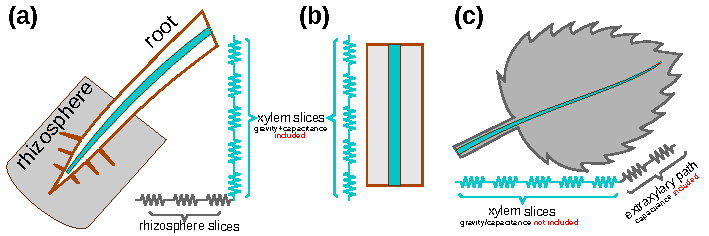
\includegraphics[width=12cm]{YW_figures/hydraulic_organs}
    \caption{Modular plant hydraulic organs: root, stem, and leaf. The pressure and flow profiles in each organ is represented by a series of xylem elements. \textbf{(a)} A root layer contains a rhizosphere component and root xylem in series. Rhizosphere component lies between the root xylem and soil. Gravitational pressure drop and water capacitance are accounted for in root xylem. \textbf{(b)} Stem hydraulics contains only stem xylem. Gravitational pressure drop and water capacitance are accounted for in stem xylem. \textbf{(c)} A leaf contains leaf xylem and an extraxylary component in series. No gravitational pressure drop or water capacitance is accounted for in leaf xylem. Instead, water capacitance locates in the leaf extraxylary path.}
    \label{fig:hydraulic_organs}
\end{figure*}




\subsection{Hydraulic system}
\par Plant organism in ``PlantHydraulics.jl'' includes a multiple layer roots (1--$\infty$ layers in parallel), an optional trunk, and an multiple layer canopy (1--$\infty$ layers in parallel). Each canopy layer has an optional branch (stem) and a leaf hydraulic organ in series. To enable a quick setup, we predefine several general organism types: ``TreeLikeOrganism'', ``PalmLikeOrganism'', and ``GrassLikeOrganism''. The differences (also see Figure \ref{fig:hydraulic_systems}) are that
\begin{itemize}
    \item ``TreeLikeOrganism'' includes multiple root layers, a trunk, and multiple stem+leaf canopy layers;
    \item ``PalmLikeOrganism'' includes multiple root layers, a trunk, and multiple leaf-only canopy layers;
    \item ``GrassLikeOrganism'' includes multiple root layers, and multiple leaf-only canopy layers.
\end{itemize}

\par \noindent Note that trunk belongs to stem organ, and all stem hydraulic properties apply to trunk.

\begin{figure*}[ht]
    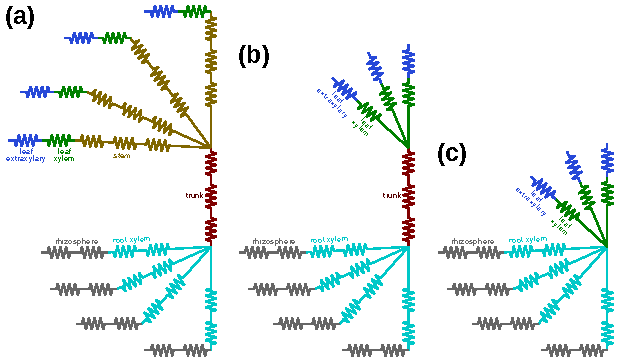
\includegraphics[width=12cm]{YW_figures/hydraulic_systems}
    \caption{Predefined plant types in ``PlantHydraulics.jl''. \textbf{(a)} Tree-like plant organism contains multiple root layers, a trunk, and multiple stem+leaf canopy layers. \textbf{(b)} Palm-like organism contains multiple root layers, a trunk, and multiple leaf-only canopy layers. \textbf{(c)} Grass-like organism contains multiple root layers, and multiple stem+leaf canopy layers.}
    \label{fig:hydraulic_systems}
\end{figure*}




\section{Vulnerability curve}

\subsection{Soil and Rhizosphere}
\par Rhizosphere is treated as soil in ``PlantHydraulics.jl'', and soil moisture retention curve is used as the vulnerability curve (VC) for rhizosphere. Also, when soil/rhizosphere re-hydrates, soil/rhizosphere hydraulic conductance will recover. Note that soil moisture retention curve relates soil water content to soil metric potential, and the metric potential varies with water temperature. Therefore, we use the metric potential normalized to 25 $^\circ$C in our model to force the one-to-one correlation to use with soil moisture retention curve, but use the temperature corrected potential to compute pressure profile. ``PlantHydraulics.jl'' supports two types of soil moisture retention curve following the formulations from \cite{brooks1964hydraulic} and \cite{van1980closed}.

\par The \cite{brooks1964hydraulic} formulation reads
\begin{equation}
    \RWCEff = \dfrac{\Theta - \ThetaR}{\ThetaS - \ThetaR} = 
              \left( \dfrac{\PsiSat}{\PsiRef} \right) ^ {\dfrac{1}{b}}
\end{equation}
\begin{equation}
    \dfrac{\KRhizo}{\KRhizoMax} = \RWCEff ^ {2b + 3}
\end{equation}
\par \noindent where $\RWCEff$ is the effective relative soil water content, $\ThetaS$ is the soil water content at soil saturation, $\Theta$ is the soil water content, $\ThetaR$ is the residual soil water content, $\PsiSat$ is the soil water metric potential at soil saturation, $\PsiRef$ is the soil metric potential at the given $\Theta$ at 25 $^\circ$C, $b$ is an exponent for given soil type, $\KRhizo$ is the rhizosphere hydraulic conductance at given $\Theta$, and $\KRhizoMax$ is the maximal rhizosphere hydraulic conductance at soil saturation.

\par The \cite{van1980closed} formulation reads
\begin{equation}
    \RWCEff = \dfrac{\Theta - \ThetaR}{\ThetaS - \ThetaR} = 
              \left[ \dfrac{1}{1 + \left( -\alpha \PsiRef \right) ^ n} \right] ^ m
\end{equation}
\begin{equation}
    \dfrac{\KRhizo}{\KRhizoMax} =
        \sqrt{\RWCEff} \cdot \left[ 1 - \left(1 - \RWCEff ^ {1/m} \right) ^ m \right] ^ 2
\end{equation}
\par \noindent where $\alpha$, $m$, and $n$ ($m = 1 - 1/n$) are soil type dependent constants.

\par Note that for both formulations, $\RWCEff$ relates the soil metric potential normalized to 25 $^\circ$C. The actual soil/rhizosphere metric potential is
\begin{equation}
    \PsiRhizo = \PsiRef \cdot \dfrac{\gamma}{\GammaRef}
\end{equation}
\par \noindent where $\gamma$ is the surface tension of liquid water, and $\GammaRef$ is the liquid water surface tension at 25 $^\circ$C. Surface tension of liquid water is computed using
\begin{equation}
    \gamma = k_\text{ST} \cdot 
             \left( 1 - \dfrac{T}{T_\text{crit}} \right) ^ {u_\text{ST}} \cdot
             \left[ 1 + b_\text{ST} \cdot \left( 1 - \dfrac{T}{T_\text{crit}} \right) \right]
    \label{eq:surface_tension}
\end{equation}
\par \noindent where $T$ is water temperature in K, $k_\text{ST}$ = 0.2358 N m$^{-2}$, $u_\text{ST}$ = 1.256, $b_\text{ST}$ = $-$0.625, and $T_\text{crit}$ = 647.096 K \citep{petrova2014revised}.

\par Hydraulic conductance is also temperature dependent (including $\KRhizo$, $\KRhizoMax$, and xylem hydraulic conductances), as the liquid water viscosity decreases with higher liquid water temperature. The temperature correction over any hydraulic conductance ($K$) is made using $K = K_{25} \cdot \text{RV}(T)$, where $K_{25}$ is the hydraulic conductance at 25 $^\circ$C, and RV($T$) is the viscosity relative to 25 $^\circ$C:
\begin{equation}
    \text{RV}(T) = \dfrac{\exp \left( \dfrac{B_\text{VIS}}{T} + C_\text{VIS}T + D_\text{VIS}T^2 \right)}
                         {\exp \left( \dfrac{B_\text{VIS}}{T_{25}} + C_\text{VIS}T_{25} + D_\text{VIS}T_{25}^2 \right)}
    \label{eq:viscosity_correction}
\end{equation}
\par \noindent where and $T_{25}$ = 298.15 K (25 $^\circ$C), $B_\text{VIS}$ = 4209 K, $C_\text{VIS}$ = 0.04527 K$^{-1}$, and $D_\text{VIS}$ = $-3.376 \times 10^{-5}$ K$^{-2}$ \citep{reid1987properties}.




\subsection{Xylem}
\par ``PlantHydraulics.jl'' adopts the air-seeding hypothesis to describe the xylem resistance to drought induced cavitation \citep{sperry1988mechanism}. Air-seeding theory posits that cavitation occurs when pressure (note that we use term ``pressure'' in xylem hydraulics) difference between liquid water in conduit lumen and air exceeds the threshold capillary pressure can withstand. Therefore, as the pore size of the pit membrane stays unchanged, the pressure difference threshold increases with higher surface tension (namely lower temperature, equation \ref{eq:surface_tension}). Again, to force the one-to-one correlation between xylem water pressure and xylem hydraulic conductance, we use the xylem VC normalized to a reference temperature at 25 $^\circ$C. Xylem VC is represented by Weibull function in ``PlantHydraulics.jl''.

\par By default, a single Weibull function is used to describe xylem VC:

\begin{equation}
    \dfrac{\KX}{\KXMax} = \exp \left[ -\left( -\dfrac{\PX}{B} \cdot \dfrac{\GammaRef}{\gamma} \right) ^ C \right]
    \label{eq:weibull_k_ratio}
\end{equation}

\par \noindent where $\KX$ and $\KXMax$ are xylem hydraulic conductance and maximum xylem hydraulic conductance at given water temperature (see equation \ref{eq:viscosity_correction}), $\PX$ is the xylem water pressure, and $B$ and $C$ are Weibull function parameters. Yet, equation \ref{eq:weibull_k_ratio} assumes that there is no drought legacy effect (previous xylem cavitation). Therefore, we modify equation \ref{eq:weibull_k_ratio} to address the problem

\begin{equation}
    \dfrac{\KX}{\KXMax} =
        \exp \left[ -\left( -\dfrac{ \min \left( \PX \cdot \dfrac{\GammaRef}{\gamma}, \PHistory \right)}{B} \right) ^ C \right]
    \label{eq:drought_history}
\end{equation}

\par \noindent where $\PHistory$ is the most negative $\PX \cdot \dfrac{\GammaRef}{\gamma}$ the xylem slice has experienced.

\par ``PlantHydraulics.jl'' also supports dual-Weibull formatted VC, for example, when fibers bridge flow path \citep{cai2014recalcitrant} and when cavitation fatigue occurs \citep{feng2015investigations}. The dual-Weibull formation is
\begin{equation}
    \dfrac{\KX}{\KXMax} =
        p_1 \cdot \exp \left[ -\left( -\dfrac{ \min \left( \PX \cdot \dfrac{\GammaRef}{\gamma}, \PHistory \right)}{B_1} \right) ^ {C_1} \right] + 
        (1 - p_1) \cdot \exp \left[ -\left( -\dfrac{ \min \left( \PX \cdot \dfrac{\GammaRef}{\gamma} , \PHistory \right)}{B_2} \right) ^ {C_2} \right]
    \label{eq:dual_weibull}
\end{equation}
\par \noindent where $p_1$ is the fraction of the first VC segment corresponds to $B_1$ and $C_1$, and $1 - p_1$ is the fraction of the second VC segment corresponds to $B_2$ and $C_2$. Note that both $\KX$ and $\KXMax$ changes with temperature as suggested by equation \ref{eq:viscosity_correction}.




\subsection{Extraxylary}
\par Water needs to move from xylem to wet leaf mesophyll cell surface, where evaporation occurs, either from symplastic or apoplastic pathways. As such, water pressure decreases from leaf xylem water pressure to leaf apoplastic water pressure ($\PApo$, we refer to the apoplastic pressure at the air-water interface). When $\PApo$ decreases, cell shrink in volume because of the decreasing cell turgor pressure (see section \ref{section:capacitance}), and the cell walls and membranes are less permeable to water, and thus extraxylary conductance to water decreases \citep{buckley2015does, buckley2017sites}. The extraxylary conductance is often more limiting and vulnerable to decreasing $\PApo$ \citep{scoffoni2017outside}. Yet, a lower $\PApo$ does not necessarily result in more damage to xylem because xylem cavitation is subjected to xylem pressure $\PX$. Furthermore, loss in extraxylary conductance ought to recover when leaf cells rehydrate as it is a result of cell expanding and shrinking.

\par Extraxylary conductance response to leaf apoplastic pressure has various forms from linear correlation to exponent and sigmoid shapes \citep{scoffoni2017outside}. Nevertheless, we use the general Weibull function to describe the various forms of linearity or non-linearity, which can be done by varying the $C$ parameter of the Weibull function
\begin{equation}
    \dfrac{\KEx}{\KExMax} = \exp \left[ -\left( -\dfrac{\PEx}{B} \right) ^ C \right]
    \label{eq:extraxylary_vc}
\end{equation}
\par \noindent where $\KEx$ is the hydraulic conductance of the extraxylary path, and $\KExMax$ is the maximal extraxylary hydraulic conductance (both $\KEx$ and $\KExMax$ are subject to viscosity correction [equation \ref{eq:viscosity_correction}]), and $\PEx$ is the extraxylary water pressure at the site. Note here that equation \ref{eq:extraxylary_vc} differs from equation \ref{eq:weibull_k_ratio} in that water pressure is not normalized by surface tension because the declining extraxylary conductance is not due to air seeded cavitation. Note that in equation \ref{eq:extraxylary_vc}, we use extraxylary water pressure, rather than extraxylary water potential, to calculate extraxylary hydraulic conductance (see section \ref{section:capacitance} for the reason).




\subsection{Capacitance\label{section:capacitance}}
\par Water capacitance in hydraulic organs may buffer flow rate in xylem and extraxylary paths, and modeling the capacitance dynamics is important to best represent the water transport process. At steady state, when water exchange between capacitance tissues and xylem conduit is minimal, and the correlation between water pressure and water capacitance is known as pressure volume curve (PV curve).

\par For any given plant capacitance tissue, water potential can be simplified as the sum of turgor pressure ($\PsiP$), osmotic potential ($\PsiO$), and gravimetric potential ($= \rho gh$, $\rho$: density of water, $g$: gravity, $h$: height above ground):
\begin{equation}
    \Psi = \PsiP + \PsiO + \rho gh
    \label{eq:pv_curve_general}
\end{equation}

\par $\PsiP$ typically decreases linearly with lower relative water content \citep[RWC;][]{tyree1972measurement, bartlett2012determinants}; When RWC is lower than a threshold ($\RWCTLP$), $\PsiP = 0$. Therefore, $\PsiP$ is a piece-wise function of RWC:
\begin{equation}
    \PsiP= \left\{
            \begin{array}{lr} 
                \epsilon \cdot \left( \RWC - \RWCTLP \right)    & \RWC > \RWCTLP \\
                0                                               & \RWC \leq \RWCTLP
            \end{array}
          \right.
\end{equation}
\par \noindent where $\epsilon$ is the bulk modulus of elasticity.

\par $\PsiO$ is proportional to the ratio between total number of osmoles in cells ($\NO$) and total water volume in cells:
\begin{equation}
    \PsiO = -\dfrac{\NO RT}{\VMAX \cdot \left( \RWC - \RWCApo \right)}
    \label{eq:pv_curve_psi_o}
\end{equation}
\par \noindent where $R$ is the gas constant, $T$ is water temperature in K, $\VMAX$ is the maximal water volume when $\Psi - \rho gh = \PsiP + \PsiO = 0$, and $\RWCApo$ is the apoplastic water content relative to $\VMAX$. Note that equation \ref{eq:pv_curve_psi_o} assumes apoplastic water volume stays constant.

\par Combining equations \ref{eq:pv_curve_general}---\ref{eq:pv_curve_psi_o}, the correlation between RWC and $\Psi$ is given:
\begin{equation}
    \Psi = \left\{
            \begin{array}{lr} 
                \epsilon \cdot \left( \RWC - \RWCTLP \right) - \dfrac{\NO RT}{\VMAX \cdot \left( \RWC - \RWCApo \right)} + \rho gh & \RWC > \RWCTLP \\
                -\dfrac{\NO RT}{\VMAX \cdot \left( \RWC - \RWCApo \right)} + \rho gh                                               & \RWC \leq \RWCTLP
            \end{array}
        \right.
    \label{eq:pv_curve_Psi}
\end{equation}
\par \noindent At equilibrium, xylem water potential ($\PsiX$) equals symplastic water potential and the apoplastic potential
\begin{equation}
    \PsiX = \PX + \rho gh = \PsiO + \PsiP + \rho gh = \PApo + \rho gh
\end{equation}
\par \noindent The xylem pressure at equilibrium equals the apoplastic pressure, and is computed using
\begin{equation}
    \PX = \PApo = \left\{
            \begin{array}{lr} 
                \epsilon \cdot \left( \RWC - \RWCTLP \right) - \dfrac{\NO RT}{\VMAX \cdot \left( \RWC - \RWCApo \right)} & \RWC > \RWCTLP \\
                -\dfrac{\NO RT}{\VMAX \cdot \left( \RWC - \RWCApo \right)}                                               & \RWC \leq \RWCTLP
            \end{array}
        \right.
    \label{eq:pv_curve_Psi_x}
\end{equation}
\par \noindent and xylem water pressure (or apoplastic pressure, $\PTLP$) at turgor loss point is
\begin{equation}
    \PTLP = -\dfrac{\NO RT}{\VMAX \cdot \left( \RWCTLP - \RWCApo \right)}
    \label{eq:pv_curve_TLP}
\end{equation}




\subsection{Water potential and pressure}
\par We remind readers that the $\rho gh$ term in equations \ref{eq:pv_curve_general} and \ref{eq:pv_curve_Psi} is required if water potential is used. For example, for a tree with xylem water pressure of $-$0.1 MPa at the tree base (ground, $\rho gh = 0$), the water potential if approximately $-$0.1 MPa as the osmotic potential can be neglected. If there is no transpiration flow or capacitance release/refill in the xylem at all, a leaf at the height of 10 m has a gravity potential $\rho gh \approx 0.1$ MPa whereas the leaf xylem water pressure $\Psi_\text{x} = -0.2$ MPa, and the total leaf xylem water potential is $-$0.1 MPa. As leaf xylem water is in equilibrium with leaf cells, leaf cells have a gravity potential of 0.1 MPa and a total water potential of $-$0.1 MPa ($\PsiO + \PsiP = -0.2$ MPa, water pressure in cells is turgor pressure). In this case, interpreting something like ``leaf water potential is $-$0.2 MPa'' is incorrect, and a correct expression is ``leaf xylem water pressure is $-$0.2 MPa''. Thus, one needs to be cautious when using terms like water potential and water pressure.

\par In ``PlantHydraulics.jl'', soil/rhizosphere retention curves are used against soil metric potential (water pressure, not soil water potential which also contains osmotic water potential and gravity potential); xylem vulnerability curves are used against xylem water pressure; and pressure volume curves are used with xylem water pressure (in root and stem) and leaf extraxylary water pressure (leaf).




\section{Flow and pressure profiles}

\subsection{Root, stem, and leaf}
\par A root layer consists of a rhizosphere and xylem in series, and we assume water temperature in the layer is constant throughout the flow path and capacitance ($T_\text{root}$). As there is no capacitance enables in the rhizosphere layer, flow rate through the rhizosphere ($E_\text{rhizo}$) is constant, and water temperature equals the soil temperature ($T_\text{soil}$). We compute the pressure drop along the rhizosphere path numerically by dividing the rhizosphere into $N_\text{rhizo}$ layers ($\Delta P_\text{i}$ for each slice). With a known soil metric potential (equivalent to soil water pressure, $P_\text{soil}$), we are able to calculate the water pressure at the end of each slice ($P_\text{rhizo,i}$):

\begin{equation}
    P_\text{rhizo,i} = P_\text{soil} + \sum_{1 \leq j \leq N_\text{rhizo}} \left( \Delta P_\text{i} \right)
\end{equation}

\par \noindent and the water pressure at the end of the root xylem is when $i = N_\text{rhizo}$. $\Delta P_\text{i}$ is calculated using

\begin{equation}
    \Delta P_\text{i} = 
        -\dfrac{E_\text{rhizo}}{k_\text{rhizo,i}} =
        -\dfrac{E_\text{rhizo} \cdot N_\text{rhizo}}
               {K_\text{rhizo,max} \cdot \text{RV}(T) \cdot \text{RK}(P_{\text{rhizo,i}-1})}
\end{equation}

\par \noindent where $k_\text{rhizo,i}$ is the hydraulic conductance in the rhizosphere slice, $K_\text{rhizo,max}$ is the maximal hydraulic conductance of the whole rhizosphere at 25 $^\circ$C, RK($P_{\text{rhizo,i}-1}$) is the relative hydraulic conductance at a given soil metric potential $P_{\text{rhizo,i}-1}$, and $P_{\text{rhizo,i}-1} = P_\text{soil}$ when $i = 1$. Iterating $i$ from 1 to $N_\text{rhizo}$ gives $P_\text{rhizo}$, which is then used to calculate the flow and pressure profiles in root xylem.

\par Xylem water capacitance in each root xylem slice may buffer the flow rate through the slice. The incoming flow rate ($E_\text{in}$) and outgoing flow rate ($E_\text{out}$) may differ, and the difference ($E_\text{out} - E_\text{in}$) is the water released from xylem capacitance (capacitance refills if the difference $< 0$). For a capacitance with its RWC, the xylem pressure at equilibrium with the given RWC can be computed using equation \ref{eq:pv_curve_Psi_x} as $P_\text{x}^{*}(\text{RWC})$, where the $^{*}$ denotes that the pressure is calculated equilibrium pressure. The pressure difference between $P_\text{x}(\text{RWC})$ and xylem water pressure $P_\text{x}$ drives the capacitance release/refill for the $i$th xylem slice:

\begin{equation}
    E_\text{out,i} - E_\text{in,i} = \left( P_\text{x}^{*}(\text{RWC}_\text{i}) - P_\text{x,i} \right) \cdot k_\text{capacity}
    \label{eq:flow_profile}
\end{equation}

\par \noindent where $k_\text{capacity}$ is the water exchange conductance between capacitance and xylem water (temperature correction also applies), and $E_\text{in,i} = E_\text{rhizo}$ where $i = 1$. Iterating $i$ through all the xylem slices (1--$N_\text{xylem}$) gives the xylem flow rate and capacitance buffer rate in each xylem slice. With the known xylem flow rates, xylem pressure at the end of each slice can be computed using

\begin{equation}
    P_\text{x,i} = P_\text{rhizo} + \sum_{1 \leq j \leq N_\text{xylem}} \left( \Delta P_\text{i} \right) + \PsiO
\end{equation}

\par \noindent where $\PsiO$ is the osmotic water potential in the rhizosphere (equals that in the corresponding soil layer). Note that $\PsiO$ in soil is temperature dependent (equation \ref{eq:pv_curve_psi_o}), and thus a correction needs to be made when accounting for non-zero $\PsiO$. $\Delta P_\text{i}$ is calculated using

\begin{equation}
    \Delta P_\text{i} =
        -\dfrac{E_\text{out,i}}{k_\text{xylem,i}} - \rho g h_\text{i} =
        -\dfrac{E_\text{out,i} \cdot N_\text{xylem}}
               {K_\text{xylem,max} \cdot \text{RV}(T) \cdot \text{RK}(P_{\text{x,i}-1})} - \rho g h_\text{i}
\end{equation}

\par \noindent where $k_\text{xylem,i}$ is the xylem hydraulic conductance in the xylem slice, $h_\text{i}$ is the height change of the root xylem slice, $K_\text{xylem,max}$ is the maximal hydraulic conductance of the whole xylem at 25 $^\circ$C, $P_\text{x,i} = P_\text{rhizo}$ when $i = 1$, and RK($P_\text{x,i}$) is the relative hydraulic conductance calculated using equation \ref{eq:weibull_k_ratio}--\ref{eq:dual_weibull}. Iterating $i$ from 1 to $N_\text{xylem}$ gives the xylem end pressure, which is also known as root xylem pressure ($P_\text{root}$).

\par Similarly, xylem end pressure at the end of the stem xylem can be calculated by first calculate the flow profile in the xylem slice with respect to capacitance using equation \ref{eq:flow_profile}, and then computing the xylem end pressure using

\begin{align}
    P_\text{trunk} = P_\text{root} + \sum_{1 \leq j \leq N_\text{xylem}} \left( \Delta P_\text{i} \right) \\
    P_\text{branch} = P_\text{trunk} + \sum_{1 \leq j \leq N_\text{xylem}} \left( \Delta P_\text{i} \right)
\end{align}

\par \noindent where $P_\text{trunk}$ is the xylem pressure at the junction of trunk and branches, and $P_\text{stem}$ is the xylem pressure at the junction of leaf and branch.

\par Then with a known $E_\text{in}$ for leaf ($E_\text{out}$ for corresponding stem if exists), leaf xylem end pressure ($P_\text{leaf,x}$) can be computed using $E_\text{in,i} = E_\text{out,i}$ because there is no capacitance enabled for leaf xylem:
\begin{equation}
    P_\text{leaf,x} = P_\text{stem} + \sum_{1 \leq j \leq N_\text{xylem}} \left( \Delta P_\text{i} \right)
\end{equation}

\par \noindent With the $E_\text{out}$ from the leaf xylem as the $E_\text{in}$ for extraxylary flow path, and the equivalent $P_\text{apo}^{*}$ calculated from leaf RWC, $E_\text{out}$ for the extraxylary flow path can be computed using:

\begin{equation}
    E_\text{out} - E_\text{in} = \left[ P_\text{apo}^{*}(\text{RWC}) - P_\text{apo} \right] \cdot k_\text{capacity}
    \label{eq:flow_profile_apo}
\end{equation}

\par Then, $P_\text{apo}$ meets

\begin{equation}
    P_\text{apo} = P_\text{leaf,x} + \Delta P =
                   P_\text{leaf,x} - \dfrac{E_\text{out}}{k_\text{ex}} = 
                   P_\text{leaf,x} - \dfrac{E_\text{out}}{k_\text{ex,max} \cdot \text{RK}(P_\text{apo})}
\end{equation}

\par \noindent where RK is the relative hydraulic conductance computed using equation \ref{eq:extraxylary_vc}. We note here that though $P_\text{apo}$ does not impact xylem cavitation, $P_\text{apo}$ influences the saturation vapor pressure ($\text{VP}_\text{sat}$, known as the Kelvin equation), which is useful to compute leaf-to-air vapor pressure deficit:

\begin{equation}
    \text{VP}_\text{sat} = \text{VP}_\text{sat}^{*} \cdot \exp \left( \dfrac{P_\text{apo} V_\text{mole}}{RT} \right)
\end{equation}

\par \noindent where $\text{VP}_\text{sat}^{*}$ is the saturate vapor pressure at a flat surface, and $V_\text{mole}$ is the molar volume of liquid water.




\subsection{Steady state simulation}
\par When flow rate in plant is at steady state, there is no net water exchange between xylem (and extracellular flow path in leaves) and capacitance tissues. On the basis of mass conservation, we know that (a) water loss from each canopy layer ($E_\text{i,canopy}$ for the $i$th layer) is constant throughout the xylem and extracellular space in the canopy layer; (b) total water loss from all canopy layers gives a constant flow rate in trunk if exists ($E_\text{trunk}$); (c) total water loss from all canopy layers equals the total flow rate from all root layers; (d) water flow in each root layer ($E_\text{j,root}$ for the $j$th root layer) is constant throughout the rhizosphere and xylem in the root layer. Therefore, we have

\begin{equation}
    \sum_{1 \leq i \leq N_\text{canopy}} \left( E_\text{i,canopy} \right) =
    E_\text{trunk} =
    \sum_{1 \leq j \leq N_\text{root}} \left( E_\text{j,root} \right)
    \label{eq:flow_conservation}
\end{equation}

\par \noindent On the basis of continuous and steady state pressure profile in the flow paths, we need an extra constraint so as to partition total canopy water demand into each root layer, namely the xylem pressure at the end of the root layer ($P_\text{i,root}$) is the same for each root, and equals the root xylem pressure ($P_\text{root}$):

\begin{equation}
    P_\text{i,root} = P_\text{root}
\end{equation}

\par To compute steady state xylem pressure profile, we first sum up all the flow rate in each leaf and use it as the total flow rate out of the roots ($E_\text{target}$, equation \ref{eq:flow_conservation}). Then, we partition the total flow rate into each root layer so that each $P_\text{i,root}$ equals. To find the root flow rate partitioning, (1) we start with an initial guess ($E_\text{i,guess}$ for the flow out of $i$th root layer). (2) With the guess flow rate, we compute the root end pressure and root hydraulic resistance (sum of root hydraulic resistance for each xylem slice, $R_\text{i,root} = \sum \left[ 1 / k_\text{xylem,j} \right]$) for each root layer. (3) We adjusted the guess flow rate at each root layer by $E_\text{i,guess} = E_\text{i,guess} - \left[ \dfrac{\sum \left( P_\text{i,root} \right)}{N_\text{root}} - P_\text{i,root} \right] / R_\text{i,root}$. (4) As the sum of all guess flow rates in root layers may differ from the target total flow rate, we adjust the flow rate again by $E_\text{i,guess} = E_\text{i,guess} - \left( \sum E_\text{i,guess} - E_\text{target} \right) \cdot \dfrac{1 / R_\text{i,root}}{\sum \left( 1 / R_\text{i,root} \right)}$. (5) We repeat step 2--4 until xylem end pressure for each root equals. With the flow rate in each flow path element, we are able to calculate the pressure profile within the hydraulic system.




\subsection{Non-steady state simulation}
\par When flow rate in plant is at non-steady state, there is water exchange between xylem flow path and capacitance tissues (e.g., xylem conduit and surrounding parenchyma cells). Though flow rate may differ among adjacent flow path element (including xylem slice and extraxylary component), mass conservation in each flow path element applies (equations \ref{eq:flow_profile} and \ref{eq:flow_profile_apo}).

\par To compute non-steady state flow and xylem pressure profiles, we first update the flow profile in plant hydraulic system. (1) We calculate the water exchange rate for each capacitance enable flow path element using water status from previous time instant as $\Delta E = \left[ P_\text{apo}^{*}(\text{RWC}) - P_\text{apo} \right] \cdot k_\text{capacity}$ (for leaf, equation \ref{eq:flow_profile_apo}) or $\Delta E = \left[ P_\text{x}^{*}(\text{RWC}_\text{i}) - P_\text{x,i} \right] \cdot k_\text{capacity}$ (for xylem, see equation \ref{eq:flow_profile}). (2) We use 
(1) For each canopy layer, we calculate water exchange with the capacitance tissue as $\Delta E = \left[ P_\text{apo}^{*}(\text{RWC}) - P_\text{apo} \right] \cdot k_\text{capacity}$ using current transpiration rate ($E_\text{leaf}$) and water status from previous time instant. (2) We compute flow rate into the leaf extraxylary path using current transpiration rate ($E_\text{leaf}$) and $\Delta E$ as $E_\text{in} = E_\text{leaf} - \Delta E$, and then use use $E_\text{in}$ as the $E_\text{out}$ and $E_\text{in}$ for the leaf xylem and $E_\text{out}$ of the last stem xylem slice if present (because there is no capacitance for leaf xylem). (3) We compute $E_\text{in}$ of the stem xylem slice, and use it as $E_\text{out}$ for the previous slice. (4) We repeat step 3 until we get the flow rate into the first stem slice (if present; otherwise, use $E_\text{in}$ of the leaf xylem). (5) Summing up all the flow rate into the stem (if present; otherwise, use sum of flow rate into the leaf xylem) gives us the flow rate out of the trunk (if present; otherwise, use the rum of flow rate into leaf directly in step 7). (6) Repeat step 3 for the trunk until we get the flow rate into the first stem slice (equals to the total flow rate out of the roots).

\par Computing non-steady state flow rates in the roots also requires that each root xylem end pressure equals. Therefore, we need to partition total flow rate among each root layer. We use similar algorithm used in the steady state flow calculation. (1) We start with an initial guess flow rate out of the last root xylem slice for each root layer. (2) With the guessed $E_\text{out}$, we compute the flow rates within all root xylem slice and rhizosphere component. (3) With the flow rate profile, we compute the root xylem end pressure ($P_\text{i,root}$) and total hydraulic resistance ($R_\text{i,root}$) along each root. (4) We adjust the guess flow rate using $E_\text{i,guess} = E_\text{i,guess} - \left[ \dfrac{\sum \left( P_\text{i,root} \right)}{N_\text{root}} - P_\text{i,root} \right] / R_\text{i,root}$. (5) We then make corrections over the guess flow rates so that their sum equals the target flow rate: $E_\text{i,guess} = E_\text{i,guess} - \left( \sum E_\text{i,guess} - E_\text{target} \right) \cdot \dfrac{1 / R_\text{i,root}}{\sum \left( 1 / R_\text{i,root} \right)}$. (6) We repeat step 2--5 until root xylem end pressure equals.

\par With the updated flow rates within each flow path element, we are able to calculate water pressure at each element. We also update the water contents in each capacitance tissue using $\text{RWC} = \text{RWC} + \dfrac{\Delta E \cdot \Delta t}{V_\text{max}}$, where $\Delta t$ is the time interval.


%\bibliography{references.bib}






\chapter{Carbon Cycle}

- Phenology
- Allocation
- Respiration

\section{Land C balance}
\begin{equation}
\frac{d\bf{C_{biomass}}}{dt} = A - R_{auto} + \bf{I_{biomass}} - \bf{M} - \bf{D_{biomass}}
\end{equation}

\begin{equation}
\frac{d\bf{C_{DOM}}}{dt} = \bf{M} + \bf{I_{DOM}} -  \bf{R_{het}} - \bf{D_{DOM}}
\end{equation}

-

-These are summary equations.

- Cbiomass and CDOM are vectors of all live biomass and DOM states. 

- Internal transfers $I$ are conservative sources (?), all other terms are  conservative sources and sinks.


\section{Autotrophic Respiration}

ANorton: To collate and synthesize approaches from other models and identify a first-order approach to autotrophic respiration. Possibly create a table that documents the components of autotrophic respiration. Thinking about the split between maintenance and growth respiration, accounting for leaf dark respiration, turnover of living tissues (linked to litter production?), new growth. 


Autotrophic respiration is considered the sum of respiratory losses of carbon (produced as $CO_2$) from all plant organs. This includes respiratory losses from plant organs that photosynthesize (autotrophic/photosynthetic materials, typically only leaves) and those that do not (heterotrophic materials, typically wood, stem, and roots). It determines the bridge between the production of substrates through photosynthesis and the growth of a plant. These respiratory losses are the necessary consumption of energy generated by the plant to support growth, maintenance and transport processes (Amthor and Baldocchi, 2001, Terrestrial Higher Plant Respiration and Net Primary Production). Over any given period the gross primary production (GPP) minus the autotrophic respiration dictates the net carbon uptake by plants, termed net primary production (NPP), which is the carbon available for allocation to plant carbon pools. Together with GPP this determines the plant carbon-use efficiency (CUE) which is defined as the ratio of net primary productivity (NPP) to gross primary productivity (GPP) or equivalently: (GPP - $R_a$) / GPP. 

For leaf respiration the choice of model can substantially impact predictions of the plant carbon balance, and there is no strong evidence for the use of any specific model whether empirical or more complex (Thomas et al., doi: 10.1029/2019MS001679). 

The paradigm in our understanding and mathematical representation of autotrophic respiration is that of the distinction between "growth" respiration and "maintenance" respiration (Amthor, 2000, doi: 10.1006/anbo.2000.117). This conceptual framework separates the total plant respiration rate into two components, growth respiration rate ($R_g$) and maintenance respiration rate ($R_m$):

\begin{equation}
\label{e:rauto_conceptual_gmp}
    R_a = R_g + R_m = g_R G + m_R W
\end{equation}

In this general formulation $G$ is the growth rate of new biomass, $g_R$ is the respiratory carbon released per unit $G$, $W$ is the dry mass of mature tissues, and $m_R$ is the maintenance respiration coefficient. The variable $m_R$ represents the respiratory cost of maintaining existing biomass per unit time (g C g C-1 day-1). In principle $g_R$ (g C g C-1) incorporates the respiratory costs of the processes that facilitate plant growth such as biosynthesis, ion uptake, nitrogen assimilation, and transport of substrates within the plant (Amthor and Baldocchi, 2001). 

The maintenance respiration ($R_m$) is generally considered the amount of carbon released in the turnover of labile substrates, active intracellular transport (maintaining solute gradients), and repair and acclimation processes in response to external forces (e.g. pests, environmental change). Commonly, models relate $R_m$ to nitrogen dynamics as it presumably processes involving proteins. It is also highly sensitive to temperature. 

The growth respiration ($R_g$) is the amount of carbon released from growing new elements, where labile substrates are converted to more structural pools (with lower turnover rates). While difficult to measure $R_g$ experimentally, there is little evidence that the coefficient $g_R$ is temperature sensitive (Johnson and Thornley, 1985, Annals of Botany, 55, p. 1-24). In particular, separating the effects of temperature on carbon supply in $G$ and $R_g$ is very difficult. It has been suggested that the ratio of the two (i.e. the carbon cost $g_R$) may be independent of temperature (Johnson and Thornley, 1985, Annals of Botany, 55, p. 1-24).

The pitfalls of this conceptual framework have been outlined before (e.g. Sprugel et al., 1995, Respiration from Organ to Stand Level). First, the process of respiration (i.e. oxidation of carbohydrates) is the same whether that energy is used for maintenance or growth processes. Second, it is very difficult to measure these two components independently. Third, plants can store the carbon produced through photosynthesis, whereas this approach assumes instantaneous respiratory losses in $R_g$. In other words, $R_g$ can, in principle have a time-delay between the production (GPP) and consumption of carbon substrates due to storage in labile substrate pools which is not considered in Eq. \ref{e:rauto_conceptual_gmp}. 

Respiration from leaves is a major component in total plant respiration, accounting for roughly half of total $R_a$ (Atkin et al., 2007, https://doi.org/10.1111/j.1469-8137.2007.02011.x). While it is difficult to determine experimentally how much of leaf respiration can be considered growth and how much can be considered maintenance, it is typically included in the maintenance respiration component. Nevertheless, there will be a transition from growth-dominated leaf respiration toward maintenance-dominated respiration as leaves go from young to mature (Atkin et al., 2017). The Farquhar photosynthesis models requires understanding of the leaf respiration rate in the daytime, defined as non-photorespiratory mitochondrial $CO_2$ release in the light, abbreviated as $R_d$ or $R_{day}$ (Farquhar et al., 1980; Brooks and Farquhar, 1985). This is distinguished from measurements of leaf respiration in darkness, or nighttime leaf respiration ($R_n$). Leaf respiration during the daytime is different to that at nighttime and undergoes a number of different metabolic pathways that can interact with photosynthesis, photorespiration, and nitrogen assimilation (for a review see Tcherkez et al., 2017, doi: 10.1111/nph.14816). Daytime leaf respiration also undergoes light inhibition (Tcherkez et al., 2017, doi: 10.1111/nph.14816), hence it is not easily inferred from $R_n$. 

From work in early phenomenological it was noticed that $R_d$ is closely related to nitrogen content and temperature (de Wit et al., 1970; also see Amthor, 2000, doi: 10.1006/anbo.2000.117) perhaps due to close relations to protein turnover. Many terrestrial models still apply empirical relationships between leaf nitrogen content and $R_d$ along with functions that adjust for temperature dependencies (Atkin et al., 2017, $https://doi.org/10.1007/978-3-319-68703-2_6$). Some terrestrial models instead apply empirical relationships between overall metabolic rate and $R_d$ by assigning scaling between the carboxylation capacity for photosynthesis ($V_{cmax}$) and $R_d$ at a standard temperature. This approach is in principle also related to nitrogen content as $V_{cmax}$ and leaf nitrogen content are often correlated. 

\subsection{Respiration mechanism}
\subsubsection{Photorespiration}
- No need to explictly model
- C3 plants only (already included in Farquhar modeLo 
DONE
\subsubsection{Dark respiration}
- C3, C4, CAM (we can ignore, make clear anyway, impossible to measure)

\subsection{Respiration type}

Contrasting climatic controls (to elaborate)

\subsubsection{Maintenance (Metabolic?)}

- Leaf respiration - related to Rd in Farquhar model (probably needs to include inhibition in light). Consider this the maintenance respiration term in leaves. With its own temperature dependence or the same used in the photosynthesis model. 

- Living stem - related to amount of living stem biomass, as carbon or nitrogen. With temperature dependence. 

- Living root - related to amount of living stem biomass, as carbon or nitrogen. With temperature dependence. 

- Fine root - related to amount of living stem biomass, as carbon or nitrogen. With temperature dependence. 

For a simple approach, write down maintenance respiration coefficients (with their temperature dependence functions) for each of the living tissue pools. 

The maintenance respiration is a function of the living biomass of the plant as follows

\begin{equation}
\label{e:rauto_maintenance_general}
    R_m^i = W^i m_R^i
\end{equation}

where $W^i$ is the dry biomass (g C m-2) of pool $i$, and $m_R^i$ is a maintenance respiration coefficient for pool $i$ (g C g C-1 day-1). In its simplest formulation Eq. \ref{e:rauto_maintenance_general} assumes one living biomass pool and one corresponding maintenance coefficient. In more complex formulations, different maintenance respiration costs can be considered for different pools and Eq. \ref{e:rauto_maintenance_general} is applied to each live biomass pool, then summed over each pool to give the total $R_m$. 

\subsubsection{Growth}

Commonly growth respiration is modelled as a fraction of $GPP$ minus $R_m$. In other words, it includes the carbon cost of building new tissues. This represents the respiratory losses associated with building new tissues. The respiratory costs for different plant organs is likely to be different (for a discussion see Sprugel et al., 1995). Nevertheless, many biosphere models assume a constant respiratory carbon cost of about 10-12\% for new growth based on limited experimental work on glucose (McDermitt and Loomis, 1981). This ignores the additional carbon (energy) expenditure required for other processes involved in building new tissues such as transport (others?). 

For a simple approach, $GPP$ and $R_m$ are simulated first, then one can apply a growth respiration coefficient to the remainder as follows: 

\begin{equation}
\label{e:rauto_growth_general}
    R_g = g_R G = g_R ( GPP - R_m )
\end{equation}

In principle, different tissues will have different growth costs (lipids, carbohydrates, others) - this coefficient can vary from about 0.10 to 0.45 (Penning de Vries et al., 1983). We can optionally have one of these equations per carbon allocation flux term (depends on the number of plant pools). 

An alternative approach is to compute $R_g$ alongside the fluxes of carbon during allocation from the labile carbon pool to the other vegetation carbon pools. This approach means that some fraction of carbon assimilation through photosynthesis is not lost immediately through $R_g$, but rather that carbon can be released through $R_g$ at a later time when allocation actually occurs. The assumption that some fraction of GPP at time $t$ is respired through growth also at time $t$ seems to be based on convenience. Studies that have tried to study growth and maintenance respiration individually cannot determine whether these fluxes are releasing new carbon or old carbon that would have passed through the labile pool first (e.g. Ryan et al., 1995, Oecologia, 101, p. 133-140). Nevertheless, optimality principles suggest that allocation of carbon to different plant organs (i.e. pools such as leaf, root and stem) will vary over time. 

Two differing hypotheses are proposed. 

First is that $R_g$ is represented as a constant fraction of GPP - $R_m$. This hypothesis implies that the carbon costs of growth due to respiratory losses are not dependent on . 

Second is that $R_g$ is coupled to the allocation fluxes. The carbon costs of growth due to respiratory losses are dependent upon 

\subsection{Temperature dependencies}

A couple of options:

1) The Q10 approach is common. This ignores high-temperature reductions. 

\begin{equation}
\label{e:phenology_lai_discrete}
    k(T) = k_{opt} Q_{10}^{\frac{T - T_{opt}}{10}}
\end{equation}

2) The peaked Arrhenius function is a particularly useful and widely applicable approach to modeling the temperature dependency of metabolic processes (e.g. Medlyn et al., 2002, https://doi.org/10.1046/j.1365-3040.2002.00891.x). 

\begin{equation}
\label{e:phenology_lai_discrete}
    k(T) = k_{opt} \frac{H_d exp(\frac{H_a(T - T_{opt})}{T R T_{opt}} }{H_d - H_a (1 - exp(\frac{H_d(T - T_{opt})}{T R T_{opt}}))}
\end{equation}

This function has four parameters, $k_{opt}$ is the rate constant at the optimum temperature, $T_{opt}$ is the optimum temperature, $H_a$ is the rate of exponential increase below $T_{opt}$ (in kJ mol-1) and $H_d$ is the rate of exponential decrease above $T_{opt}$ (in kJ mol-1). In general $H_d$ is left fixed often because of limited data available above the temperature optimum. 

Benefits:

 - in a single function it includes (i) Arrhenius function that describes the exponential dependence of a metabolic rate to temperature, and (ii) high-temperature down-regulation. 

 - one form of this function includes a parameter for the temperature optimum of the metabolic rate, which could itself be regulated to account for acclimation processes over longer 
 time-scales 

\subsection{Nitrogen dependencies}

The relationship between autotrophic respiration and nitrogen is important from the perspective of analyses of traits and process understanding. This largely stems from the fact that respiration involves turnover of proteins (nitrogen-rich) and processes related to proteins. In principle, if we use maintenance respiration coefficients for each living tissue pool we can have a placeholder for nitrogen content of each living tissue. In a first, simple approach, the maintenance respiration term would be g C g C-1 day-1, while with nitrogen pools included it could become g C g N-1 day-1 (similar to CLM5).

\section{Leaf Phenology}

The quantity of leaves within the canopy is computed based on the generic phenology model described in \citet{Knorr2010}. 

\subsection{A General Spatial Approach}

The typical approach to modeling leaf phenology is by using one or more growth triggers (or thresholds) that transition the vegetation into or out of an active growth state. This is problematic given that this is often modeled using a discrete formulation such as an if statement. In reality, plants over a given region (or grid cell) do not reach these thresholds simultaneously. There is likely to be a distribution of individual plants with individual triggers, resulting in a relatively smooth transition toward the new growth state. The model of \citet{Knorr2010} assumes that the "spatial variability within a grid cell is entirely the result of differences in the threshold parameter defining the trigger, effectively subsuming impacts of small‐scale climatic variability under the same". To model this, the threshold parameter is represented as a normal distribution in space. While this is a convenient solution to the problem, it is also grounded in the understanding that "dormancy in buds is not a single state, but rather a range of states that can vary within an individual over the course of the activity-dormancy cycle, between individuals of a species, and also between species" \citep{Cooke2012}. 

We can first consider a general formulation for the LAI of an individual plant ($\tilde{\Lambda}$) that switches into a growth phase when air temperature ($T$) exceeds that plants threshold temperature ($\tilde{T_{\phi}}$). When this condition is not met, the plant is not in an active growth phase. This can be represented by a differential equation in time ($t$) as follows:

\begin{equation}
\label{e:phenology_lai_discrete}
    \frac{d\tilde{\Lambda}(t)}{dt} = 
    \begin{cases}
    f_1,  &  \text{if }T \geq \tilde{T}_{\phi},\\
    f_2, &  \text{else, }
    \end{cases}
\end{equation}

where $f_1$ and $f_2$ are some arbitrary functions describing the state of the plant during the growth phase and senescent phase, respectively. This discrete formulation means that the relationship between LAI and the threshold parameter $\tilde{T}_{\phi}$ is non-differentiable at the transition point of the threshold. To overcome this, the spatially integrated LAI considers all individual plants within a grid cell, each with their own threshold parameter. Thus, the spatially integrated LAI ($\Lambda$) is represented by:

\begin{equation}
\label{e:phenology_lai_integral_temp}
    \frac{d\Lambda(t)}{dt} = f_1 \int_{-\infty}^{T} p(\tilde{T}_{\phi}) \; d\tilde{T}_{\phi} - f_2 \left( 1 - \int_{-\infty}^{T} p(\tilde{T}_{\phi}) \; d\tilde{T}_{\phi} \right)
\end{equation}

where $p$ is equal to a spatial Gaussian probability density function of the threshold variable $\tilde{T}_{\phi}$, with a mean $T_{\Phi}$ and standard deviation $T_r$. Additional threshold conditions can be included such as the day length ($t_d$). In the case of two threshold conditions (temperature and day length), the spatially integrated LAI is represented by:

\begin{equation}
\label{e:phenology_lai_integral_tempdaylength}
    \frac{d\Lambda(t)}{dt} = f_1 \int_{-\infty}^{T} \int_{-\infty}^{t_d} p(\tilde{T}_{\phi}) \; q(\tilde{t_{c}}) \; d\tilde{T}_{\phi} \; d\tilde{t_{c}} - f_2 \left( 1 - \int_{-\infty}^{T} \int_{-\infty}^{t_d} p(\tilde{T}_{\phi}) \; q(\tilde{t_{c}}) \; d\tilde{T}_{\phi} \; d\tilde{t_{c}} \right)
\end{equation}

where $q$ is equal to a spatial Gaussian probability density function of the threshold variable $\tilde{t_{c}}$, with a mean $t_{c}$ and standard deviation $t_r$. 

We can simplify this equation if we consider the integral as a cumulative distribution function ($\Phi$), again described by the deviation from the mean. This, again, is the cumulative distribution in space, not time. This results in the following: 

\begin{equation}
\label{e:phenology_lai_integral_simple}
    \frac{d\Lambda(t)}{dt} = f_1 f - f_2 (1 - f)
\end{equation}
with

\begin{empheq}[box=\eqnbox]{equation}\label{e:phenology_lai_cdf}
    f = \int_{-\infty}^{T} p(\tilde{T}_{\phi}) \; d\tilde{T}_{\phi} \; \int_{-\infty}^{t_d} q(\tilde{t_{c}}) \; d\tilde{t_{c}} \; = \; \Phi \left( \frac{T - T_{\phi}}{T_r} \right) \Phi \left( \frac{t_d - t_c}{t_r} \right),
\end{empheq}

alternatively, the temperature and day-length functions can be computed separately as follows: 

\begin{equation}
\label{e:phenology_lai_cdf_temp-daylength}
\begin{split}
    f(T) & = \Phi \left( \frac{T - T_{\phi}}{T_r} \right) \\
    f(t_d) & = \Phi \left( \frac{t_d - t_c}{t_r} \right)
\end{split}
\end{equation}

This represents the spatially integrated LAI response to threshold variables, $T$ and $t_d$, where $f$ varies between 0 and 1. Given that we're integrating over individual plants within a grid cell, the variable $f$ represents the fraction of plants in an active growth state. 

\subsection{Temporal Evolution of LAI}

With the general spatial approach described above we require some formulation for the evolution of the LAI of an individual plant over time. This requires a formulation for the two states of a plant, active growth ($f_1$) and a senescent state ($f_2$). \citet{Knorr2010} uses a relatively simple formulation for these two states and assumes the following: "leaf growth starts immediately and is not limited by substrate availability, such as LAI itself; and growth stops if a target LAI is reached that is in balance with the environmental limitations". This target LAI is given by $\Lambda_{max}$. Thus, the active growth function takes the form:

\begin{equation}
\label{e:phenology_lai_f1}
    f_1 = \xi (\Lambda_{max} - \Lambda)
\end{equation}

Where $\xi$ is a linear growth constant that describes the increase in LAI per unit time shortly after bud burst. This rate is assumed to be independent of the current NPP, as often the initial growth following bud burst is determined by the previous growing seasons carbon gains. 

For plants outside of their growth stage, a simplest possible formulation is the following:

\begin{equation}
\label{e:phenology_lai_f2}
    f_2 = \frac{\Lambda}{\tau_L}
\end{equation}

Where the parameter $\tau_L$ represents leaf longevity (in days) i.e. how quickly leaves are shed or whether they stay inactive until the next growing season. 

Combining these two growth state formulations with spatially integrated LAI as in Eq. \ref{e:phenology_lai_integral_simple}, we get

\begin{equation}
\label{e:phenology_lai_integral_f1f2}
    \frac{d\Lambda(t)}{dt} = \xi \big( \Lambda_{max} - \Lambda(t) \big) f - \frac{\Lambda(t)}{\tau_L} (1 - f)
\end{equation}

\citet{Knorr2010} goes further, simplifying this differential equation to provide a convenient form for integrating Eq. \ref{e:phenology_lai_integral_f1f2}. They define 

\begin{empheq}[box=\eqnbox]{equation}\label{e:phenology_lai_r}
    r = \xi f + \frac{(1 - f)}{\tau_L}
\end{empheq}

%\begin{equation}
%\label{e:phenology_lai_r}
%    \textcolor{blue}{ r = \xi f + \frac{(1 - f)}{\tau_L} }
%\end{equation}

and 

\begin{empheq}[box=\eqnbox]{equation}\label{e:phenology_lai_Lambda_lim}
    \Lambda_{lim} = \frac{\xi \Lambda_{max} f}{r}
\end{empheq}

%\begin{equation}
%\label{e:phenology_lai_Lambda_lim}
%    \textcolor{blue}{ \Lambda_{lim} = \frac{\xi \Lambda_{max} f}{r} }
%\end{equation}

In order to prevent $\Lambda_{lim}$ from going to to zero, it is kept positive by using an exponentially smoothed maximum of Eq. \ref{e:phenology_lai_Lambda_lim} and a small positive value, using

\begin{equation}
\label{e:phenology_lai_lambdalim_expsmoothed}
    \nu(x,y,x_0) = 
    \begin{cases}
        x + x_0 e^{-(x-y)/x_0-1},  &  \text{if } x \geq (y - x_0),\\
        y, &  \text{else, }
    \end{cases}
\end{equation}

where $\nu$ is the smoothed exponential maximum function, $x$ = $\Lambda_{lim}$ from Eq. \ref{e:phenology_lai_Lambda_lim}, $y$ = 1e-9, and $x_0$ = 5e-3. 

With the definition of $r$ and $\Lambda_{lim}$, Eq. \ref{e:phenology_lai_integral_f1f2} becomes:

\begin{equation}
\label{e:phenology_lai_final}
\begin{split}
    \frac{d\Lambda(t)}{dt} & = \xi \Lambda_{max} f - r \Lambda(t) \\
    & = r \big( \Lambda_{lim} - \Lambda(t) \big)
\end{split}
\end{equation}

With this, the term $r$ represents the inverse rate of growth ($days^{-1}$) and $\Lambda_{lim}$ represents the LAI limit of the current time-step to which $r$ approaches. 

The implementation of Eq. \ref{e:phenology_lai_final} within the model is done by updating the LAI incrementally. Thus, Eq. \ref{e:phenology_lai_final} has the solution:

\begin{empheq}[box=\eqnbox]{equation}\label{e:phenology_lai_incremental}
    \Lambda(t + \Delta t) = \Lambda_{lim} - \big( \Lambda_{lim} - \Lambda(t) \big) e^{-r \Delta t}
\end{empheq}

%\begin{equation}
%\label{e:phenology_lai_incremental}
%    \textcolor{blue}{ \Lambda(t + \Delta t) = \Lambda_{lim} - \big( \Lambda_{lim} - \Lambda(t) \big) e^{-r \Delta t} }
%\end{equation}

Where $\Delta t$ is the time step of the leaf phenology model, usually daily. 

\subsection{Temperature Limitations}

The model of \citet{Knorr2010} avoids the use of growing degree day sums which are typically used in models to simulate temperature requirements for growth of cold climate vegetation. Such a formulation has two pitfalls. First, these approaches typically yield a discrete transition into a growth phase, triggered when the growing degree days exceed a pre-defined critical value. This can lead to non-differentiable transitions. Second, many models that employ this approach must arbitrarily reset the accumulated growing degree days variable each winter or at the beginning of the calendar year (e.g. for northern hemisphere vegetation). \citet{Knorr2010} takes a slightly different approach using a smooth formulation to account for temperature and/or day length thresholds. 

For temperature, this approach applies exponentially declining weights to temperature going back in time, equivalent to an exponentially declining memory of a plant to temperature. To represent this, the phenology determining temperature $T$ is formulated as

\begin{equation}
\label{e:phenology_lai_temp}
\begin{split}
    T(t) & = \frac{ \int_{-\infty}^{0} T_{air} (t+\tilde{t}) e^{\tilde{t} / \tau_m} d \tilde{t} }{ \int_{-\infty}^{0} e^{\tilde{t} / \tau_m} d \tilde{t}}  \\
    & = \frac{1}{ \tau_m } \int_{-\infty}^{0} T_{air} (t + \tilde{t}) e^{\tilde{t} / \tau_m} d \tilde{t} \\
    & = \frac{1}{ \tau_m } e^{-t / \tau_m}  \int_{-\infty}^{0} T_{air} (t') e^{t' / \tau_m} d t'
\end{split}
\end{equation}

where $\tau_m$ is the period over which $T$ is averaged. A sensible value for $\tau_m$ is 30 days. 

Again, the implementation of this equation is simplified by bringing it into an incremental form:

\begin{equation}
\label{e:phenology_lai_temp_incremental}
\begin{split}
    T(t+\Delta t) & = \frac{1}{ \tau_m } e^{-(t+\Delta t) / \tau_m}  \int_{-\infty}^{(t+\Delta t)} T_{air} (t') e^{t' / \tau_m} d t'  \\
    & = \frac{1}{ \tau_m } e^{-\Delta t / \tau_m} e^{-t / \tau_m} \bigg( \int_{-\infty}^{t} T_{air} (t') e^{t'/ \tau_m} d t' + \int_{-\infty}^{t+\Delta t} T_{air} (t') e^{t'/ \tau_m} d t' \bigg) \\
    & = e^{-\Delta t / \tau_m} T(t) + \frac{1}{ \tau_m } e^{-(t+\Delta t) / \tau_m} \int_{t}^{t+\Delta t} T_{air} (t') e^{t'/ \tau_m} d t' \\
\end{split}
\end{equation}

If $\Delta t$ is the time step of the leaf phenology model (usually daily) and $T_{air}$ is constant over that period, this simplifies to:

\begin{empheq}[box=\eqnbox]{equation}\label{e:phenology_lai_temp_incremental2}
    T(t+\Delta t) = e^{-\Delta t / \tau_m} T(t) + T_{air}(t) ( 1 - e^{-\Delta t / \tau_m} )
\end{empheq}

%\begin{equation}
%\label{e:phenology_lai_temp_incremental2}
%    \textcolor{blue}{ T(t+\Delta t) = e^{-\Delta t / \tau_m} T(t) + T_{air}(t) ( 1 - e^{-\Delta t / \tau_m} ) }
%\end{equation}

This allows for $T$ to be updated at each model time step rather than computed using Eq. \ref{e:phenology_lai_temp} which requires accessing variables in past (i.e. $T_{air}$ over the past 30 days). 

\subsection{Water and Structural Limitations}

In the absence of well-defined mechanisms linking plant water status to LAI, \citet{Knorr2010} develops a simple approach to modeling a water-limited LAI ($\Lambda_W$). The principle is that "leaf development will stop and leaves will be shed if there is insufficient soil water for transpiration". The precise balance of plant available soil water and water required for transpiration may be a function of the adaptations of the plant e.g. life history and genetics. This adaptation is represented by a single parameter, $\tau_W$. This parameter defines the length of time a plant will tolerate water shortages before leaf shedding. In order to maintain a given LAI (the water-limited LAI; $\Lambda_W$), the amount of transpiration that can occur over a given time period must be balanced by the plant available soil moisture ($W$) as follows:

\begin{equation}
\label{e:phenology_lai_water_1}
    E(\Lambda_W) \tau_W = W
\end{equation}

To make use of this, we require a function for the potential water loss after time $\tau_W$ as a function of LAI. In \citet{Knorr2010}, they apply a linear relationship between LAI and the potential transpiration rate $E$ with

\begin{equation}
\label{e:phenology_lai_water_2}
    E(\Lambda) \approx \frac{\tilde{E}}{\tilde{\Lambda}} \Lambda
\end{equation}

where $\tilde{E}$ is the daily mean potential rate of transpiration last computed by the model at an LAI of $\tilde{\Lambda}$. This is, however, a simple approximation of how transpiration and LAI relate. \citet{Knorr2010} notes that this may only be valid for low LAI values where net radiation drives the evapotranspiration. A more appropriate form may include a saturating function. 

Combining Eq. \ref{e:phenology_lai_water_1} and \ref{e:phenology_lai_water_2} gives:

\begin{empheq}[box=\eqnbox]{equation}\label{e:phenology_lai_water_3}
    \Lambda_W = \frac{W \tilde{\Lambda}}{\tilde{E} \tau_W}
\end{empheq}

%\begin{equation}
%\label{e:phenology_lai_water_3}
%    \textcolor{blue}{ \Lambda_W = \frac{W \tilde{\Lambda}}{\tilde{E} \tau_W} }
%\end{equation}

Under a steady $W$, if $\tilde{E}$ declines then $\Lambda_W$ increases such that water-limitation becomes weaker on LAI. Similarly, if $W$ declines

If the ratio between $W$ and $\tilde{E} \tau_W$ decreases (e.g. $W$ is smaller than $\tilde{E} \tau_W$) then $\Lambda_W$ will decline i.e. LAI becomes more water-limited. In general, as $\tau_W \xrightarrow$0, $\Lambda_W \xrightarrow$ $\infty$ as the plant assumes water will always be available for leaf growth. Thus, vegetation without any water-driven leaf phenology will have $\tau_W=0$. 

Water limitation is not the only limiting factor in growth of new leaves, so an overall maximum potential LAI is introduced with the parameter $\hat{\Lambda}$. This represents the maximum LAI possible given other constraints such as physical structure, light, or nutrients. We take the actual LAI to be the minimum of the two potentially limiting LAI values, $\Lambda_W$ and $\hat{\Lambda}$, as follows:

\begin{empheq}[box=\eqnbox]{equation}\label{e:phenology_lai_waterstructure}
    \tilde{\Lambda}_{max} = \nu \left( \hat{\Lambda}, \Lambda_W \right)
\end{empheq}

%\begin{equation}
%\label{e:phenology_lai_waterstructure}
%    \textcolor{blue}{ \tilde{\Lambda}_{max} = \nu \left( \hat{\Lambda}, \Lambda_W \right) }
%\end{equation}

Where $\nu$ is a quadratic minimum function that provides a smooth transition between $\hat{\Lambda}$ and $\Lambda_W$, defined by

\begin{equation}
\label{e:phenology_lai_waterstructure_quadsmoothed}
    \nu(x,y) = \frac{x + y - \sqrt{(x+y)^2 - 4\eta x y}}{2 \eta}
\end{equation}

where $\eta$ is the degree of smoothing, typically $\eta$ = 0.9. 

The incorporation of $\tilde{\Lambda}_{max}$ from Eq. \ref{e:phenology_lai_waterstructure} into Eq. \ref{e:phenology_lai_Lambda_lim} is not direct. We do not compute $\tilde{\Lambda}_{max}$ using only instantaneous values for $W$ and $\tilde{E}$ but instead use a time weighted integration similar to that for temperature (in Eqs. \ref{e:phenology_lai_temp} and \ref{e:phenology_lai_temp_incremental2}). Hence,

\begin{equation}
\label{e:phenology_lai_waterstructure_quadsmoothed}
    \Lambda_{max}(t) = \frac{1}{ \tau_s } e^{-t / \tau_s}  \int_{-\infty}^{0} \tilde{\Lambda}_{max} (t') e^{t' / \tau_s} d t'
\end{equation}

and this can be updated incrementally (as is done for $T$ in Eq. \ref{e:phenology_lai_temp_incremental2}) as follows

\begin{empheq}[box=\eqnbox]{equation}\label{e:phenology_lai_waterstructure_incremental}
    \Lambda_{max}(t+\Delta t) = e^{-\Delta t / \tau_s} \Lambda_{max}(t) + \tilde{\Lambda}_{max}(t) ( 1 - e^{-\Delta t / \tau_s} )
\end{empheq}

%\begin{equation}
%\label{e:phenology_lai_waterstructure_incremental}
%    \textcolor{blue}{ \Lambda_{max}(t+\Delta t) = e^{-\Delta t / \tau_s} \Lambda_{max}(t) + \tilde{\Lambda}_{max}(t) ( 1 - e^{-\Delta t / \tau_s} ) }
%\end{equation}

where $\tau_s$ is the period over which $\Lambda_{max}$ is averaged ($\tau_s$ = 30 days). In practice, $\Lambda_{max}$ from Eq. \ref{e:phenology_lai_waterstructure_incremental} is substituted into Eq. \ref{e:phenology_lai_Lambda_lim}. 


\subsection{Light Intensity Controlled Leaf Dynamics}

The leaf phenology model of \citet{Knorr2010} presents hypotheses on the control of temperature, day length, and water availability on leaf growth and senescence. Measurements of leaf phenology in tropical forests suggest another potential control, light intensity. Some studies have highlighted the relationship between increasing light intensity and leaf litterfall in the Amazon at the beginning of the dry season \citep{}. Along transects in one part of the Amazon forest, \citet{Rice2004} found that litterfall was higher with lower precipitation, potentially suggesting a role of increasing light availability. 

While water availability is likely to impose limitations on leaf phenology, the availability of light is likely to drive changes in leaf phenology as well. \citet{Kim2012} introduced this mechanism into the Ecosystem Demography model 2 (ED2). The equations are given below. 

A quick but important side note here: We must take into consideration that the ED2 model approximates sub-grid variability in canopy structure and composition by using a system of size- and age-structured partial differential equations \citep{Medvigy2009}. This sub-grid variability is designed to "approximate the ensemble mean behavior of a corresponding individual‐based stochastic gap model" \citep{Medvigy2009} i.e. it approximates the population densities of individuals of each plant type and size class that make up the grid-scale canopy. Thus, in practice ED2 implements the two equations below per plant type, per plant size class, and per sub-grid tile. It is worth noting that \citet{Weng2015} developed a potentially more favourable approach that reduces the numerical complexity used in ED2, providing an analytically tractable set of equations for modeling the sub-grid scale variability, and included a competitively optimal carbon allocation scheme under the "perfect plasticity approximation" hypothesis \citet{Franklin2020}. 

The primary mechanism is the impact of radiation on the leaf turnover rate ($\alpha_{leaf}$). Each individual plant has the $\alpha_{leaf}$ computed by:

\begin{equation}
\label{e:phenology_leafturnover_radiation}
    \alpha_{leaf} = (\alpha_1 \bar{I} + \alpha_2) \alpha_0
\end{equation}

Further to this, \citet{Kim2012} introduced a relationship between leaf longevity ($\tau_L$ in BETHY, $LL$ in ED2), the inverse of $\alpha_{leaf}$, and the maximum potential carboxylation capacity ($V_{cmax}$). This is developed from knowledge of the coordination between leaf lifespan and photosynthetic capacity \citep{Wright2004}. This relationship is represented by a sigmoidal function as follows,

\begin{equation}
\label{e:phenology_leafturnover_vcmax_coord}
    V_m = \frac{V_m^{amp}}{\big( 1 + (\frac{LL}{LL^{trans}})^{V_m^{slope}} \big)} + V_m^{min}
\end{equation}

where the minimum $V_m$ is given by $V_m^{min}$, and the maximum $V_{m}$ is given by $V_m^{min}$+$V_m^{amp}$. The $V_m^{slope}$ is the rate at which $V_m$ changes with respect to $LL$. 

\subsection{Carbon Supply Limitation}

In principle the supply of carbon (NPP) can limit the growth of new leaves and thus have some control over leaf phenology. In its simplest terms, the amount of carbon allocated to new leaves can be represented by

\begin{equation}
\label{e:phenology_lai_water_1}
C_{leaf} = f_{leaf} \; NPP \; SLA
\end{equation}

where $f_{leaf}$ is the fraction of NPP allocated to leaf development and $SLA$ is the specific leaf area (the reciprocal of leaf mass per area). 


\subsection{Leaf Shedding and Litter Production}

The model of \citet{Knorr2010} also derives the mass of leaves that are shed and hence the amount of carbon that is contributed to the leaf litter. This is calculated as

\begin{empheq}[box=\eqnbox]{equation}\label{e:phenology_lai_shed}
    C_{leaf shed} (t) = C_{dm} \; \frac{ \nu \left( (\Lambda(t) - \Lambda_{lim}(t) ) (1 - e^{-r \Delta t)}, 0.0, 0.001 \right)}{SLA} 
\end{empheq}

%\begin{equation}
%\label{e:phenology_lai_shed}
%    C_{leaf shed} (t) = C_{dm} \; \frac{ \nu \left( \Lambda_{lim}(t) - \Lambda (t) (1 - e^{-\Delta t / r)}, 0.0, 0.001 \right)}{SLA} 
%\end{equation}

where $C_{dm}$ is the carbon content of dry matter ($g C \; g \; dry \; matter^{-1}$), SLA is the specific leaf area (the reciprocal of leaf mass per area), and $\nu$ is an exponential maximum function, equivalent to Eq. \ref{e:phenology_lai_lambdalim_expsmoothed}.



\begin{table}[]
\resizebox{\textwidth}{!}{%
\begin{tabular}{lllll}
State Variables         & Description                           & Units                     & Definition                            & Typical value     \\ \hline
 $\Lambda$                    & Leaf area index & m$^2$ m$^{-2}$ & Eq. \ref{e:phenology_lai_incremental} & $0\le \Lambda \le 12$ \\
   $T$                    & Leaf phenology temperature memory &  $^{\circ}$C & Eqs. \ref{e:phenology_lai_temp_incremental2}, \ref{e:phenology_lai_cdf_temp-daylength} & $0\le T \le 50$ \\
   $t_d$                    & Day-length &  hours & Eq. \ref{e:phenology_lai_cdf_temp-daylength} & $0\le t_d \le 24$ \\
   $W$                    & Plant available soil water & mm & Eq. xx & $0\le W \le xx$ \\
   $\tilde{E}$                    & Daily potential transpiration rate & mm day^{-1} & Eq. xx & $1e-3\le \tilde{E} \le xx$ \\  [2ex]
Functions of State      & Description                           & Units                     & Definition                            & Typical value \\ \hline
    $f$                    & Fraction of plants in active growth state & - & Eqs. \ref{e:phenology_lai_cdf}, \ref{e:phenology_lai_cdf_temp-daylength} & $0\le f \le 1$  \\
    $f_1$                    & Active growth function & LAI day$^{-1}$ & Eq. \ref{e:phenology_lai_f1} & -  \\
    $f_2$                    & Senescent phase function & LAI day$^{-1}$ & Eq. \ref{e:phenology_lai_f2} & -  \\  
    $\Lambda_{max}$                    & Maximum leaf area index & m$^2$ m$^{-2}$ & Eq. xx & $0\le t_d \le 12$ \\
   $\Lambda_{lim}$                    & Leaf area index limit & m$^2$ m$^{-2}$ & Eq. xx & $1e-9\le t_d \le 12$ \\
   $\Lambda_W$                    & Water-limited leaf area index & m$^2$ m$^{-2}$ & Eq. xx & $1e-9\le \Lambda_W \le 12$ \\
   $r$                    & Inverse growth rate & days$^{-1}$ & Eq. xx & $0\le r \le 1$ \\  [2ex]
Empirical Properties      & Description                           & Units                     & Definition                            & Typical value \\ \hline
$T_{\phi}$             & Mean temperature at leaf onset       & $^{\circ}$C   & Eq. xx     & $-\infty\le T_{\phi} \le 50$   \\
$T_r$             & Spatial range (1$\sigma$) of $T_{\phi}$       & $^{\circ}$C   & Eq. xx     & $0.5\le T_{r} \le 15$   \\
$\tau_m$             & Time interval over which $T$ is averaged       & days   & Eq. \ref{e:phenology_lai_temp_incremental2}     & 30   \\
$t_c$             & Mean day length at leaf shedding       & hours   & Eq. xx     & $0\le t_c \le 24$   \\
$t_r$             & Spatial range (1$\sigma$) of $t_c$       & hours   & Eq. xx     & $0.5\le t_{r} \le 24$   \\
$\hat{\Lambda}$             & Physical maximum leaf area index       & m$^2$ m$^{-2}$   & Eq. xx     & $0.05\le \hat{\Lambda} \le 12$   \\
$\xi$             & Initial linear leaf growth rate      & days$^{-1}$   & Eq. xx     & $0.01\le \xi \le 50$   \\
$k_L$             & Inverse leaf longevity ($\tau_L$)      & days$^{-1}$   & Eq. xx     & $1e-3\le k_L \le 0.2$   \\
$\tau_W$             & Target survival time under water-deficit conditions      & days   & Eq. \ref{e:phenology_lai_water_3}     & $0\le \tau_W \le 365$   \\
$\tau_s$             & Time interval over which $\Lambda_{max}$ is averaged  & days   & Eq. \ref{e:phenology_lai_waterstructure_incremental}     & 30   \\

%\hline
\end{tabular}%
}% end resizebox
\caption{\label{t:leaf_phenology_variables}Key leaf phenology variables and parameters. See \citet{Knorr2010} and \citet{Kim2012} for further details.}
\end{table}

\section{Dead organic C states}

\subsection{Multiple pool arrangements}

-Simple formulation with no vertical transfer include two litter pools and three soil pools; complex formulation has the same carbon pools but added vertical transfer, see Figure 7.1 for the diagram of complex version.

\begin{figure}[htb]
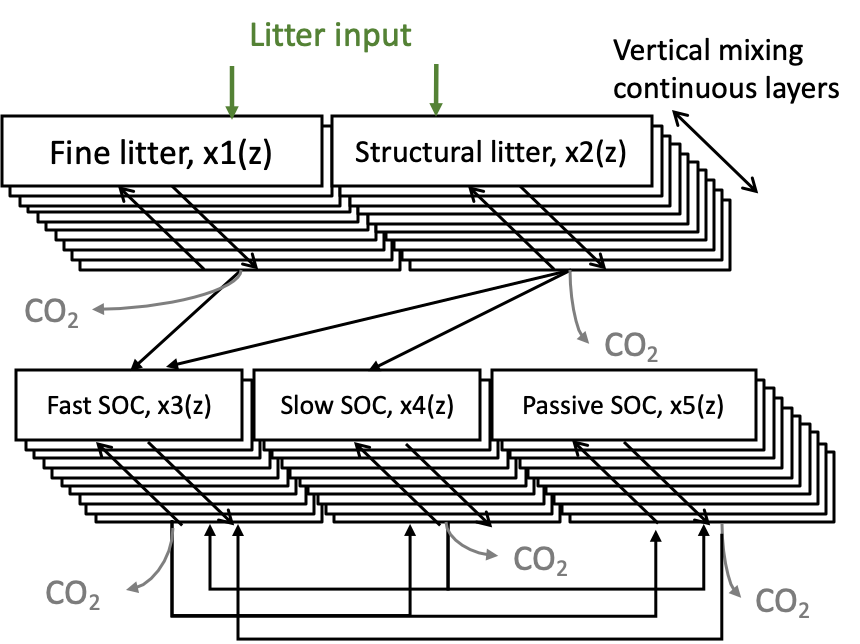
\includegraphics[width=10cm,height=10cm,keepaspectratio]{CLIMA-land/LM_figures/CLIMA_DOM_complexv2.png}
\caption{Dead organic matter schemes in CliMA Land – complexed version.}
\label{f:Dead organic matter schemes in CliMA Land – complexed version.}
\end{figure}

\subsection{Carbon balance equations}

-General equations for DOM pools (for single soil layer model structure)

\begin{equation}
\frac{dC_{i}}{dt} = B_i + \sum_{j\neq i}A_{ji}k_j\xi_iC_j - k_i\xi_iC_i
\end{equation}
    where $C_i$ is the carbon content of pool i, $B_i$ are the live C biomass inputs into the system (only non-zero for the two litter pools), the second term ($\sum_{j\neq i}A_{ji}k_j\xi_iC_j$) is the sum of C transferred in from pool j to pool i, the third term ($k_iC_i$) is the C transferred out of pool i. $k_i$ is the basal decay rate of pool i, $\xi_i$ combines the effect of environmental scalars and nitrogen limitation factor on the decay rate (shown in the next sections);$A_ji$ is the fraction of carbon allocation from pool j to pool i and $r_j$ is the respired fraction of carbon leaving the system during the transfer.

-Accounting for vertical C transfer, the balance equation is:

\begin{equation}
\frac{\partial C_i}{\partial t} = B_i(z) + \sum_{j\neq i}A_{ji}k_j(z)\xi_j(z)C_j(z) - k_i(z)\xi_i(z)C_i + \nabla(D(z)\nabla C_i) + \nabla(V(z)C_i)
\end{equation}

    where now $C_i$ is the carbon content of pool i at depth z, variables in this equation with a (z) indicate it is a parameter that the value change with depth. The last two terms represent the vertical transport, the diffusive flux and the advective fluxes, where D is diffusive coefficient, and V is advection rate.



\subsection{Parameter look-up table}
B,A,r,k,xi,D,A
\begin{figure}[htb]
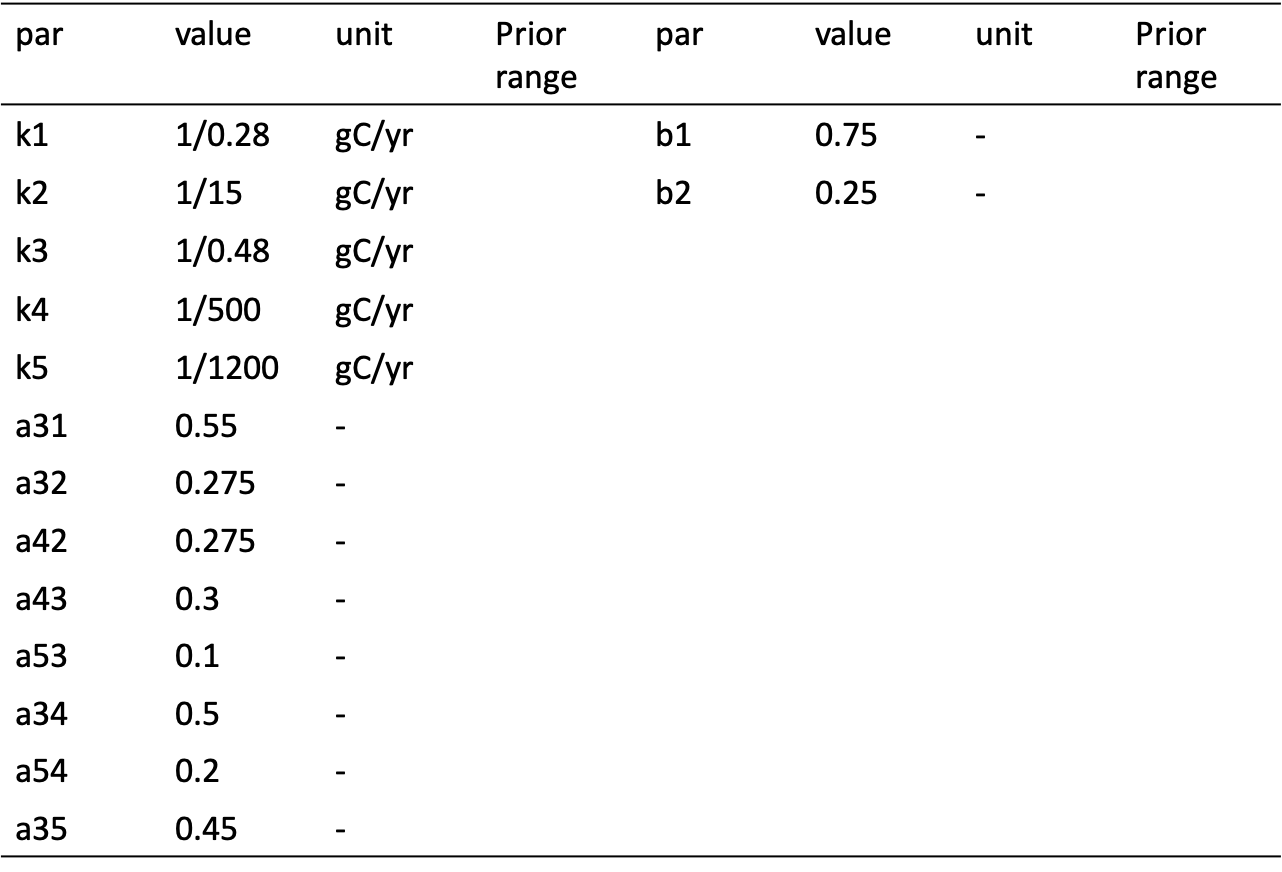
\includegraphics[width=10cm,height=10cm,keepaspectratio]{CLIMA-land/LM_figures/DOM_parlist_v2.png}
\caption{Parameters used in DOM.}
\label{f:Parameters used in DOM.}
\end{figure}

\subsection{remaining questions decide later}

-Do we include lateral movement (eg. runoff) of dissolved organic carbon (DOC) and dissolved inorganic carbon (DIC)? The C loss from runoff is on the same scale of $CH_4$ emission in a northern peatland.

\subsection{Environmental scalars}

\subsubsection{Temperature scalar}

-Q10 vs. alternative formulations

\subsubsection{Moisture scalar}
-High moisture suppression effect on aerobic respiration
-Joint aerobic and anaerobic respiration

\subsection{N limitation of decomposition fluxes}
\subsection{External N cycle}
\subsection{Methane model}
-one or multiple layers
-processes included 1)production only or 2)plus other processes (oxidation, emission pathways)


\bibliographystyle{agufull08}
\bibliography{Yujie_refs,Renato_refs,CLIMA-refs}

\chapter{Appendix}
\section{Overview of TOPMODEL}\label{Appendix:TOPMODEL}

Below we sketch the arguments of TOPMODEL; Figure~\ref{f:baseflow} illustrates the TOPMODEL problem and the variables used. The primary output of this is an expression for local water table depth as a function of topography and the mean water table depth. This can be used to determine the inundated area fraction of the surface, which is then needed for computing surface runoff. 

\begin{figure}[htb]
\centering
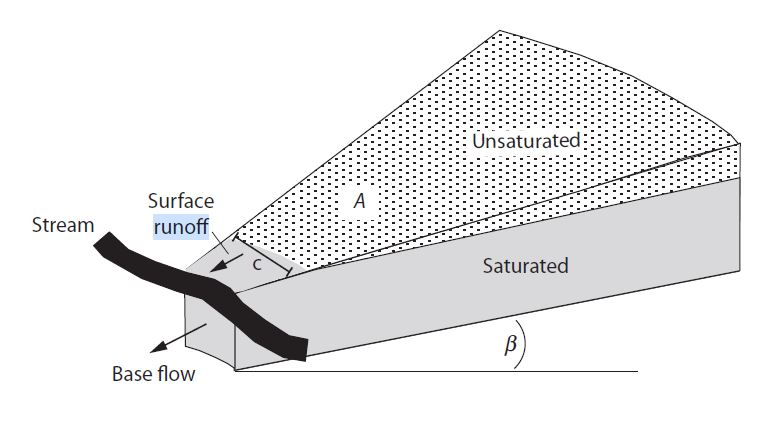
\includegraphics[width=7cm,height=7cm,keepaspectratio]{CLIMA-land/LM_figures/baseflow.JPG}
\caption{Representation of surface and subsurface runoff with the TOPMODEL approach. We model changes in topography at the subgrid scale as variations in hillslope angle $\beta$, contributing area $A$ and width $c$.  The saturated zone intersects the surface, which results in surface runoff. Baseflow in TOPMODEL flows into a river, stream or channel leaving the soil system.}
\label{f:baseflow}
\end{figure}

%Baseflow $\mathrm{(m^3/s)}$ is the rate of net losses and %gains of liquid water through horizontal movement. To %define baseflow, 
%at any point $x=(w\hat{x},l\hat{y})$, 
We start with the definition of the Darcy flux $\mathrm{(m/s)}$ (section ~\ref{s:water_balance}) at a location $(x,y, z)$. We consider only the component of the downhill slope direction projected onto the $(x,y)$ plane $\hat{x}'$, as the assumption of hydrostatic equilibrium applies in the vertical.  

\noindent We have
\begin{equation}\label{baseflow_darcy}
    \vec{d}_{l,x'}(x,y,z)=-K \hat{x}'\cdot \nabla h  
\end{equation}
%\noindent Baseflow (m$^3$/s) is then found by integrating $\vec{d}_{l,x'}$ across the coarse grid column depth and length, in z and $y'$ respectively.
%\begin{equation}
%    \vec{R}^{baseflow}_l  = \int_{y'} \int_z \vec{d}_{l,x'} dz dy'
%    \label{baseflow}
%\end{equation}
We follow TOPMODEL and make the following assumptions about \ref{baseflow_darcy}. 
\begin{enumerate}
    \item Lateral flows within the unsaturated zone are negligible, so only flows within the water table are modelled. Hence, we set $K=K_{sat}$, and integrate from the bottom of the column, $z_{bedrock}$, to the top of the water table $z_{\nabla}(x,y)$, which gives a vertically integrated discharge $\mathrm{(m^2/s}$)  in the $x'$ direction 
    \begin{align} 
   \vec{Q}_{x'}(x, y)&=-\int_{z_{\rm bedrock}}^{z_{\nabla}}(K_{sat}\hat{x}'\cdot\nabla h) dz
    \label{qlx}
    \end{align}
    \item In TOPMODEL, the local saturated hydraulic conductivity is assumed to decay exponentially with depth, to model the effect of soil compaction down to the bedrock \citep{Ambroise96}. 
    %($z_{\rm sfc}(x,y) - z$)
    \begin{equation}
        K_{sat}(x, y, z)=K_{sat}^0(x, y) \exp(-f (z_{\rm sfc}- z)),
        \label{Ksat}
    \end{equation}
    where
    \begin{itemize}
    \item $K_{sat}^0(x, y)$ local saturated hydraulic conductivity at the surface at subgrid point ($\mathrm{ms^{-1}}$);
    \item $f(x, y)$ parameter describing the reduction of saturated conductivity with depth ($\mathrm{m^{-1}}$);
    %inverse of the scale depth 
    \item $z_{\mathrm{sfc}}(x, y)$ local height of the surface ($\mathrm{m}$);
    \end{itemize}
   Note that other functions can be used instead of an exponential profile for modeling $K_{sat}$ \citep{Ambroise96}, and that changing this functional form changes the topographic index (which must be computed from a priori from a topography data set). To find the parameter $f$, we could fit an exponential function to the data for $K_{sat}(z)$, which is resolved at the coarse grid scale\footnote{It's possible an exponential will not fit well. We could explore fitting the data for $K_{\rm sat}(z)$ with other functions, or a Taylor expansion. However, the integral of $K_{\rm sat}(z)$ has to be inverted to solve for $z_\nabla$, to in turn obtain the functional form of the topographic index.}.
   \item The local water table is assumed to be parallel to the surface. This is how TOPMODEL links baseflow to topography: it implies that the local horizontal gradient of the head is related to the local slope angle $\beta$ as 
    \begin{equation}
   \hat{x}' \cdot \nabla h    = \rm tan (\beta). 
    \label{tanb}
    \end{equation}
    A future improvement could involve using a different approximation of $ \hat{x}' \cdot \nabla h$ following \citep{beven2001dynamic}, which performs better for steep slope angles. \hl{and maybe only enters when the bedrock is not flat?}
    Inserting equation \ref{tanb} and \ref{Ksat} into \ref{qlx}, 
    \begin{align}\label{int_q_runoff}
   \vec{Q}_{x'}(x) &= \mathrm{tan(\beta)} \int_{z_{\rm bedrock}}^{z_{\nabla}} K_{\rm sat}^0\exp(-f (z_{\rm sfc}- z) dz \nonumber \\
   &\approx T_0 \mathrm{tan(\beta)} \exp(-f (z_{\rm sfc}-z_{\nabla}), 
    \end{align}
    where $T(z_{\nabla}) \equiv \int_{z_{\rm bedrock}}^{z_{\nabla}} K_{\rm sat}^0\exp(-f (z_{\rm sfc}- z) dz$ is the transmissivity ($\mathrm{m^2/s}$). Note that there is an inherent contradiction in this assumption: if the slope is always parallel to the water table, then it can't intersect the surface. However, in practice, this is of no importance as we don't physically represent the river in TOPMODEL. 
    \item The transmissivity constant, defined as $T_0 = K_{sat}^0/f$, is assumed to be homogeneous across the region. This implies that the same profile for $K_{sat}$ applies across the grid, but is consistent with our using the soil type data (which determines $K_{\rm sat}$) of coarse grid element to determine the value of $f$. 
    %After integration, equation \ref{qx} then becomes 
    %\begin{align}
     %Q_x'(x') &\approx T_0 \mathrm{tan(\beta)} \exp(-f (z_{\rm sfc}-z_{\nabla})     \label{int_q_runoff}
    %\end{align}
%where $\hat{x}$ defines the direction of lateral baseflow (towards a stream, in the original TOPMODEL).
%A future improvement could involve using a different approximation of $ \hat{x}' \cdot \nabla h$ following \citep{beven2001dynamic}, to account for the effect of steep slope angles \hl{Anna: finish summarizing the improvement}. %This would yield $Q_x(x)=\sin{(b)} T(z_{\nabla})$. T(z_{\nabla})$ the local saturated transmissivity perpendicular to the slope (better to use this for steep angle) \citep{beven2001dynamic} and $T_0 = K_{sat}^0/f$ the maximum saturated transmissivity.
   
\item The saturated zone is assumed to be in quasi steady state : the volume of water entering from the surface and infiltrating downwards to the saturated zone at upslope recharge rate $i$ ($\mathrm{ms^{-1}}$) leaves it at the same rate. This net infiltration at the surface $i(z_{\mathrm{sfc}})=P-E-R_{l}$, where $P$, $E$ and $R_{l}$ are precipitation, evaporation and  surface runoff fluxes, is assumed to be spatially homogeneous at the subgrid scale. 
    \begin{equation}
        \partial S/\partial t = 0 = -\divergence \mathbf{Q}_{x'}(x) + i(z_{\mathrm{sfc}}),
    \end{equation}
    The integral of the upslope recharge rate equals the vertically integrated discharge 
    %$Q_x(x') = \int_{z_{\rm bedrock}}^{z_{\nabla}} q_x(x) dz$   at any point on the watershed (should we define this)
    \begin{equation}
        \vec{Q}_{x'}(x) = i a
        \label{mass_balance_waterhsed}
    \end{equation}
    where $a$ $(\mathrm{m^2m^{-1}})$ is the hillslope area per unit contour length feeding into the stream. 
    \end{enumerate} 

The vertically integrated flux $\vec{Q}_{x'}(x)$ can be inverted using \ref{mass_balance_waterhsed} to solve for the local water table depth, and the mean of this over the grid is then:
\begin{equation}
    \overline{z_\nabla} = \overline{z}_{\rm sfc}+ \frac{1}{f}\bigg[ \log{(i/T_0))} + \overline{\phi} \bigg],
\end{equation}
where $\phi = \log{(a/\tan{(\beta))}}$ is the topographic index, and $\overline{\phi}$ is the grid averaged value. We then use this expression to relate the local water table depth $z_{\rm sfc} - z_{\nabla}$  to the mean, using our assumptions that $i$ and $T_0$ are spatially homogeneous in the grid cell:
\begin{equation}\label{eq:wt_depth_ti}
    (z_{\rm sfc} - z_{\nabla}) = (\overline{z}_{\rm sfc}-\overline{z_{\nabla}})-\frac{1}{f}(\phi - \overline{\phi})
\end{equation}
Note that the water table depth (positive measured downwards) is zero where the water table intersects the surface. This expression for the local water table depth can also be used in Equation \eqref{int_q_runoff} to obtain lateral flow within the water table at a point along the hillslope. 

\section{Baseflow and subgrid physics}\label{Appendix:WaterTableSubGrid}
This summarizes the background for baseflow modeling as relevant to CliMA. We begin with an equation for water table height, including source and sink terms. Our goal is to understand what effect subgrid variations in water table height have on coarse grid moisture levels in soil. At the end we will discuss how these results can be applied to an equation for $\vartheta_l$.

Key assumptions:
\begin{itemize}
    \item Hydrostatic equilibrium holds in the vertical. This allows us to relate the height of the water table ($\eta$; measured from the bedrock, at $z=0$) in terms of the augmented liquid fraction.
    \item The contribution of unsaturated flow above the water table is negligible.
    \item The bed rock is flat, or that it is deep enough that slope changes in it do not greatly affect baseflow.
    \item $K = K(z)$, $\nu = \nu(z)$, and $S_s = S_s(x, y)$.
\end{itemize}

Then one can show that the equation for the height of the water table $\eta(x,y,t)$ satisfies
\begin{equation}\label{hsb}
    \nu(\eta) \partial_t \eta = \nabla \cdot ( T(\eta) \nabla \eta) + \mathcal{S_{\rm inf}} +\mathcal{S}_{\rm str}
\end{equation}
where
\begin{equation}
    T(h) \equiv \int_0^\eta K(z) dz,
\end{equation}
\begin{equation}
    \mathcal{S_{\rm inf}} \equiv (P-E-R_l) \hat{n} \cdot \hat{z}
\end{equation}
is the source due to infiltration, with $\hat{n}$ the normal to the surface of the soil.  The minus sign out front then $\mathcal{S_{\rm str}}$ is the sink due to streams, if present. Equation \eqref{hsb} is essentially the hill-slope Boussinesq equation.

\paragraph{Reduction to TOPMODEL}
TOPMODEL makes the assumption that the baseflow within the water table on a hillslope with a slope angle $\alpha$ is in steady state. If there is no stream, this implies
\begin{equation}
    \nu(\eta)\partial_t \eta=0  = \nabla \cdot T(\eta)\nabla \eta + (P-E-R_l)\hat{n} \cdot \hat{z}
\end{equation}
or, if we align our horizontal axes such that $\hat{x}$ points in the direction of the flow,
\begin{equation}
     \int d(T(\eta) \partial_x \eta) = -\int_0^x(P-E-R_l)\hat{n} \cdot \hat{z} dx
\end{equation}
We assume that at the top of the slope, at $x=0$, that there is no baseflow into the domain. We additionally assume that $P-E-R_l$ is constant across the domain, and denote it $i$, and replace $\partial_x = -\tan \alpha$ (assuming the hillslope decreases with $x$, and and the water table height is parallel to the surface, as in TOPMOEL). Then
\begin{equation}
     (T(\eta)\tan \alpha)\bigg|_x = i\int_0^x\hat{n} \cdot \hat{z} dx.
\end{equation}
If we further denote $a(x) = \int_0^x\hat{n} \cdot \hat{z} dx$ as the upstream area flowing through a unit contour length (in $\hat{y}$), then we recover the baseflow of TOPMODEL:
\begin{equation}
    T(\eta)\tan \alpha  = ia(x).
\end{equation}
Given $K(z)$, this can then (1) averaged and (2) used to express $\eta$ in terms of the mean water table height and local topography ($\tan\alpha$ and $a$). Note that following this approach to determine $\eta$ locally requires primarily the assumption of steady state. We will still make use of this, most likely.  

A further extension is to take the resulting expression for flow at stream, and then sum it over the stream length (perpendicular to $x$) to get the net loss. Note that TOPMODEL seems to assume that the water table height at the stream is zero, so that all of the flow is runoff. If there is nonzero height to the water table, we cannot treat all of the baseflow as runoff (as an example - the baseflow just above the bedrock would not runoff into a stream many meters above it). Additionally, the assumptions of TOPMODEL break down at the stream. If the water table is parallel to the surface, it can never intersect the surface, unless it intersects it everywhere. 

\paragraph{Lateral flow between columns}
We first consider how unresolved subgrid variations in the water table height affect baseflow in columns where there is no stream. We write
\begin{equation}
    \eta = \eta_0 +\eta',
\end{equation}
where $\eta_0$ is the component of $\eta_0$ resolved on large spatial scales, and $\eta'$ is the deviation from that due to small spatial scale variations. Denoting
\begin{equation}
    <f> \equiv \int_{x=0}^L \int_{y=0}^L dA f(x,y) 
\end{equation}
as the grid averaged $f$, we further assume that $<\eta'>=0$ and that \\
$<g(\eta_0) \eta'> = <g(\eta_0)><\eta'> = 0$ for any $g$, i.e. that $\eta_0$ and $\eta'$ are uncorrelated. 

Even if the hydraulic conductivity and porosity were independent of height, Equation \eqref{hsb} would be nonlinear in $\eta$, and we would end up with terms nonlinear in $\eta'$ that do not average to zero over the coarse grid scales.  

Instead, we make the simplifying assumption that $\eta'/\eta_0<<1$. If we ignore second order terms $\mathcal{O}(\eta'^2)$, the equation for $\eta$ when no sinks or sources are present reduces to:
\begin{equation}
    \bigg(\nu(\eta_0)+\eta'\partial_\eta\nu|_{\eta_0}\bigg)\partial_t \eta_0 + \nu(\eta_0)\partial_t \eta' = \nabla \cdot [(T(\eta_0)+K(\eta_0) \eta') \nabla \eta_0] + \nabla \cdot [T(\eta_0)\nabla \eta']
\end{equation}
which, when we then average over the column, reduces to
\begin{equation}
    <\nu(\eta_0)\partial_t \eta_0>  = \nabla \cdot <T(\eta_0)\nabla \eta_0>.
\end{equation}
What this indicates is that, under these assumptions, the subgrid variations in water table height do not contribute to lateral flow between columns. This is true only if the deviations are small enough to ignore $\mathcal{O}(\eta'^2)$ terms.

As an aside, our surface runoff calculations incorporate subgrid effects to determine the net water flux at the surface of the soil. In other words, the sub grid contributions to $P-E-R_l$ on the coarse grid scale are already accounted for, and we won't consider them further here. (I don't think we account for the $\hat{n} \cdot \hat{z}$ term though, meaning we assume the surface is $\approx$ flat).

\paragraph{Expression for the stream sink}
In the above, we have not accounted for the scenario where the water table height intersects the surface.

It should be possible to derive an expression for the flux of water that leaves the surface at a stream, depending on e.g. the slope of the surface, as well as the slope of the water table, and even the stream stage.  However, we will not resolve the local, minor, stream locations, or their depths. Instead, for now, we express this sink more generally as

\begin{equation}
    \mathcal{S_{\rm str}} = -\frac{\eta - z_{\rm sfc}}{\tau(\phi,...) } \mathcal{H}(\eta - z_{\rm sfc})
\end{equation}
for some appropriate value of $\tau$, which could depend on local topography $\phi$, the density of the stream network, or the main river height (rather than using $z_{\rm sfc}$, e.g.), for example. This equation holds at a point, and would need to be averaged over the column cross sectional area $A$ to apply to the coarse scale column:
\begin{equation}
    <\nu(\eta_0)\partial_t \eta_0>  = \nabla \cdot <T(\eta_0)\nabla \eta_0>-\frac{1}{A}\int dA \frac{1}{\nu_{\rm sfc}}\frac{\eta - z_{\rm sfc}}{\tau(\phi,...)} \mathcal{H}(\eta - z_{\rm sfc}).
\end{equation}


%There is also a more ``exact" expression for the sink, and if I didnt make a mistake (unlikely), it depends on $\nabla \eta-\nabla z_{\rm sfc}$. If we wanted to include a source term like this, we need the subgrid deviations in the water table slope, and subgrid deviations in surface height slope. TOPMODEL does not provide this, and in fact assumes that the two are parallel.
%Our equation solves for the height as a function of horizontal coordinate and time. We can imagine this as the equation for the height of a column with some (small) base area $L^2$. Then the sink term for that column would be
%\begin{align}
%    \mathcal{S_{\rm str}} &= -\frac{1}{L}T(\eta) (\partial_x\eta -\partial_x z) \mathcal{H}(\eta-z_{\rm sfc}).
%\end{align}
%I'm not sure about the factor of $L$. It could be something like the width of a stream. But In the derivation of the conservative term, we don't just have a sink, we have a difference in fluxes at $x$ and $x+dx$ - then dividing by $L = dx$ gives the divergence term as $dx \rightarrow 0$. It doesn't work out in the same way here.  

\paragraph{A sink term for $\vartheta_l$}
Given $\partial_t \eta$, we can return to our assumption of hydrostatic equilibrium in the vertical to write
\begin{equation}
\partial_t <\vartheta_l> = <S_s(x) \partial_t \eta>,
\end{equation}
in which case our sink term becomes
\begin{align}
    \mathcal{S_{\rm str}} &= -\frac{1}{A}\int dA \frac{S_s(x)}{\nu_{\rm sfc}}\frac{\eta - z_{\rm sfc}}{\tau(\phi,...)} \mathcal{H}(\eta - z_{\rm sfc}) \nonumber \\
\end{align}
TOPMODEL provides a probability distribution for $\eta-z_{\rm sfc}$. However, we will instead make use of the relationship between surface moisture and topographic index, as this also indicates where local conditions are inundated.

In that case, we would apply
\begin{align}
    \mathcal{S_{\rm str}} &= -\frac{1}{A}\int dA \nu_{\rm sfc}\frac{S_{\rm sfc}-1}{\tau(\phi,...)} \mathcal{H}(S_{\rm sfc} - 1) \nonumber \\
\end{align}
%For $\tau$, we could use something like $\tau = \Delta_x/K_{\rm sat} \partial_x \eta \approx \Delta_x/K_{\rm sat} \partial_x z_{\rm sfc}$, or drop the factor depending on slope.

\end{document}








\section{Stuff from Previous Version}

In the soil, heat follows a 1D vertical heat diffusion:
\begin{equation}
     \frac{\partial (C_s T_s) }{\partial t} = \frac{\partial }{\partial z}\kappa \frac{\partial T_s }{\partial z} + S_T
\end{equation}
where $C_s$--the volumetric heat capacity--is the product of soil density and specific heat capacity, i.e.  $C_s = \rho_s c_s$, and are defined in subsequent sections, and $\kappa$ is the thermal conductivity of the soil, $S_T$ are sources of heat such as phase change. Phase change heating rate can be expressed as: 
\begin{equation}
    S_T = \rho L_m \frac{\partial \theta_{i}}{\partial t}_{|{\rm ice-liquid \ change}}.
    \end{equation}
with $\frac{\partial \theta_{i}}{\partial t}_{|{\rm ice-liquid \ change}}$ the local rate of change of liquid into ice. 


We can combine the phase change with temperature defining a total energy $H=C_s T_s+ \rho L_m \theta_{i}$ and an ice-conserved temperature $T_{\rm ice}=H/C_s$ to get:
\begin{equation}
     \frac{\partial H }{\partial t}  =  \frac{\partial }{\partial z}\kappa \frac{\partial T_s }{\partial z}
\end{equation}
or using $T_{\rm ice}$:
\begin{equation}
     \frac{\partial (C_s T_{\rm ice})}{\partial t} =  \frac{\partial }{\partial z}\kappa \frac{\partial T_s }{\partial z}
\end{equation}

\begin{figure}[htb]
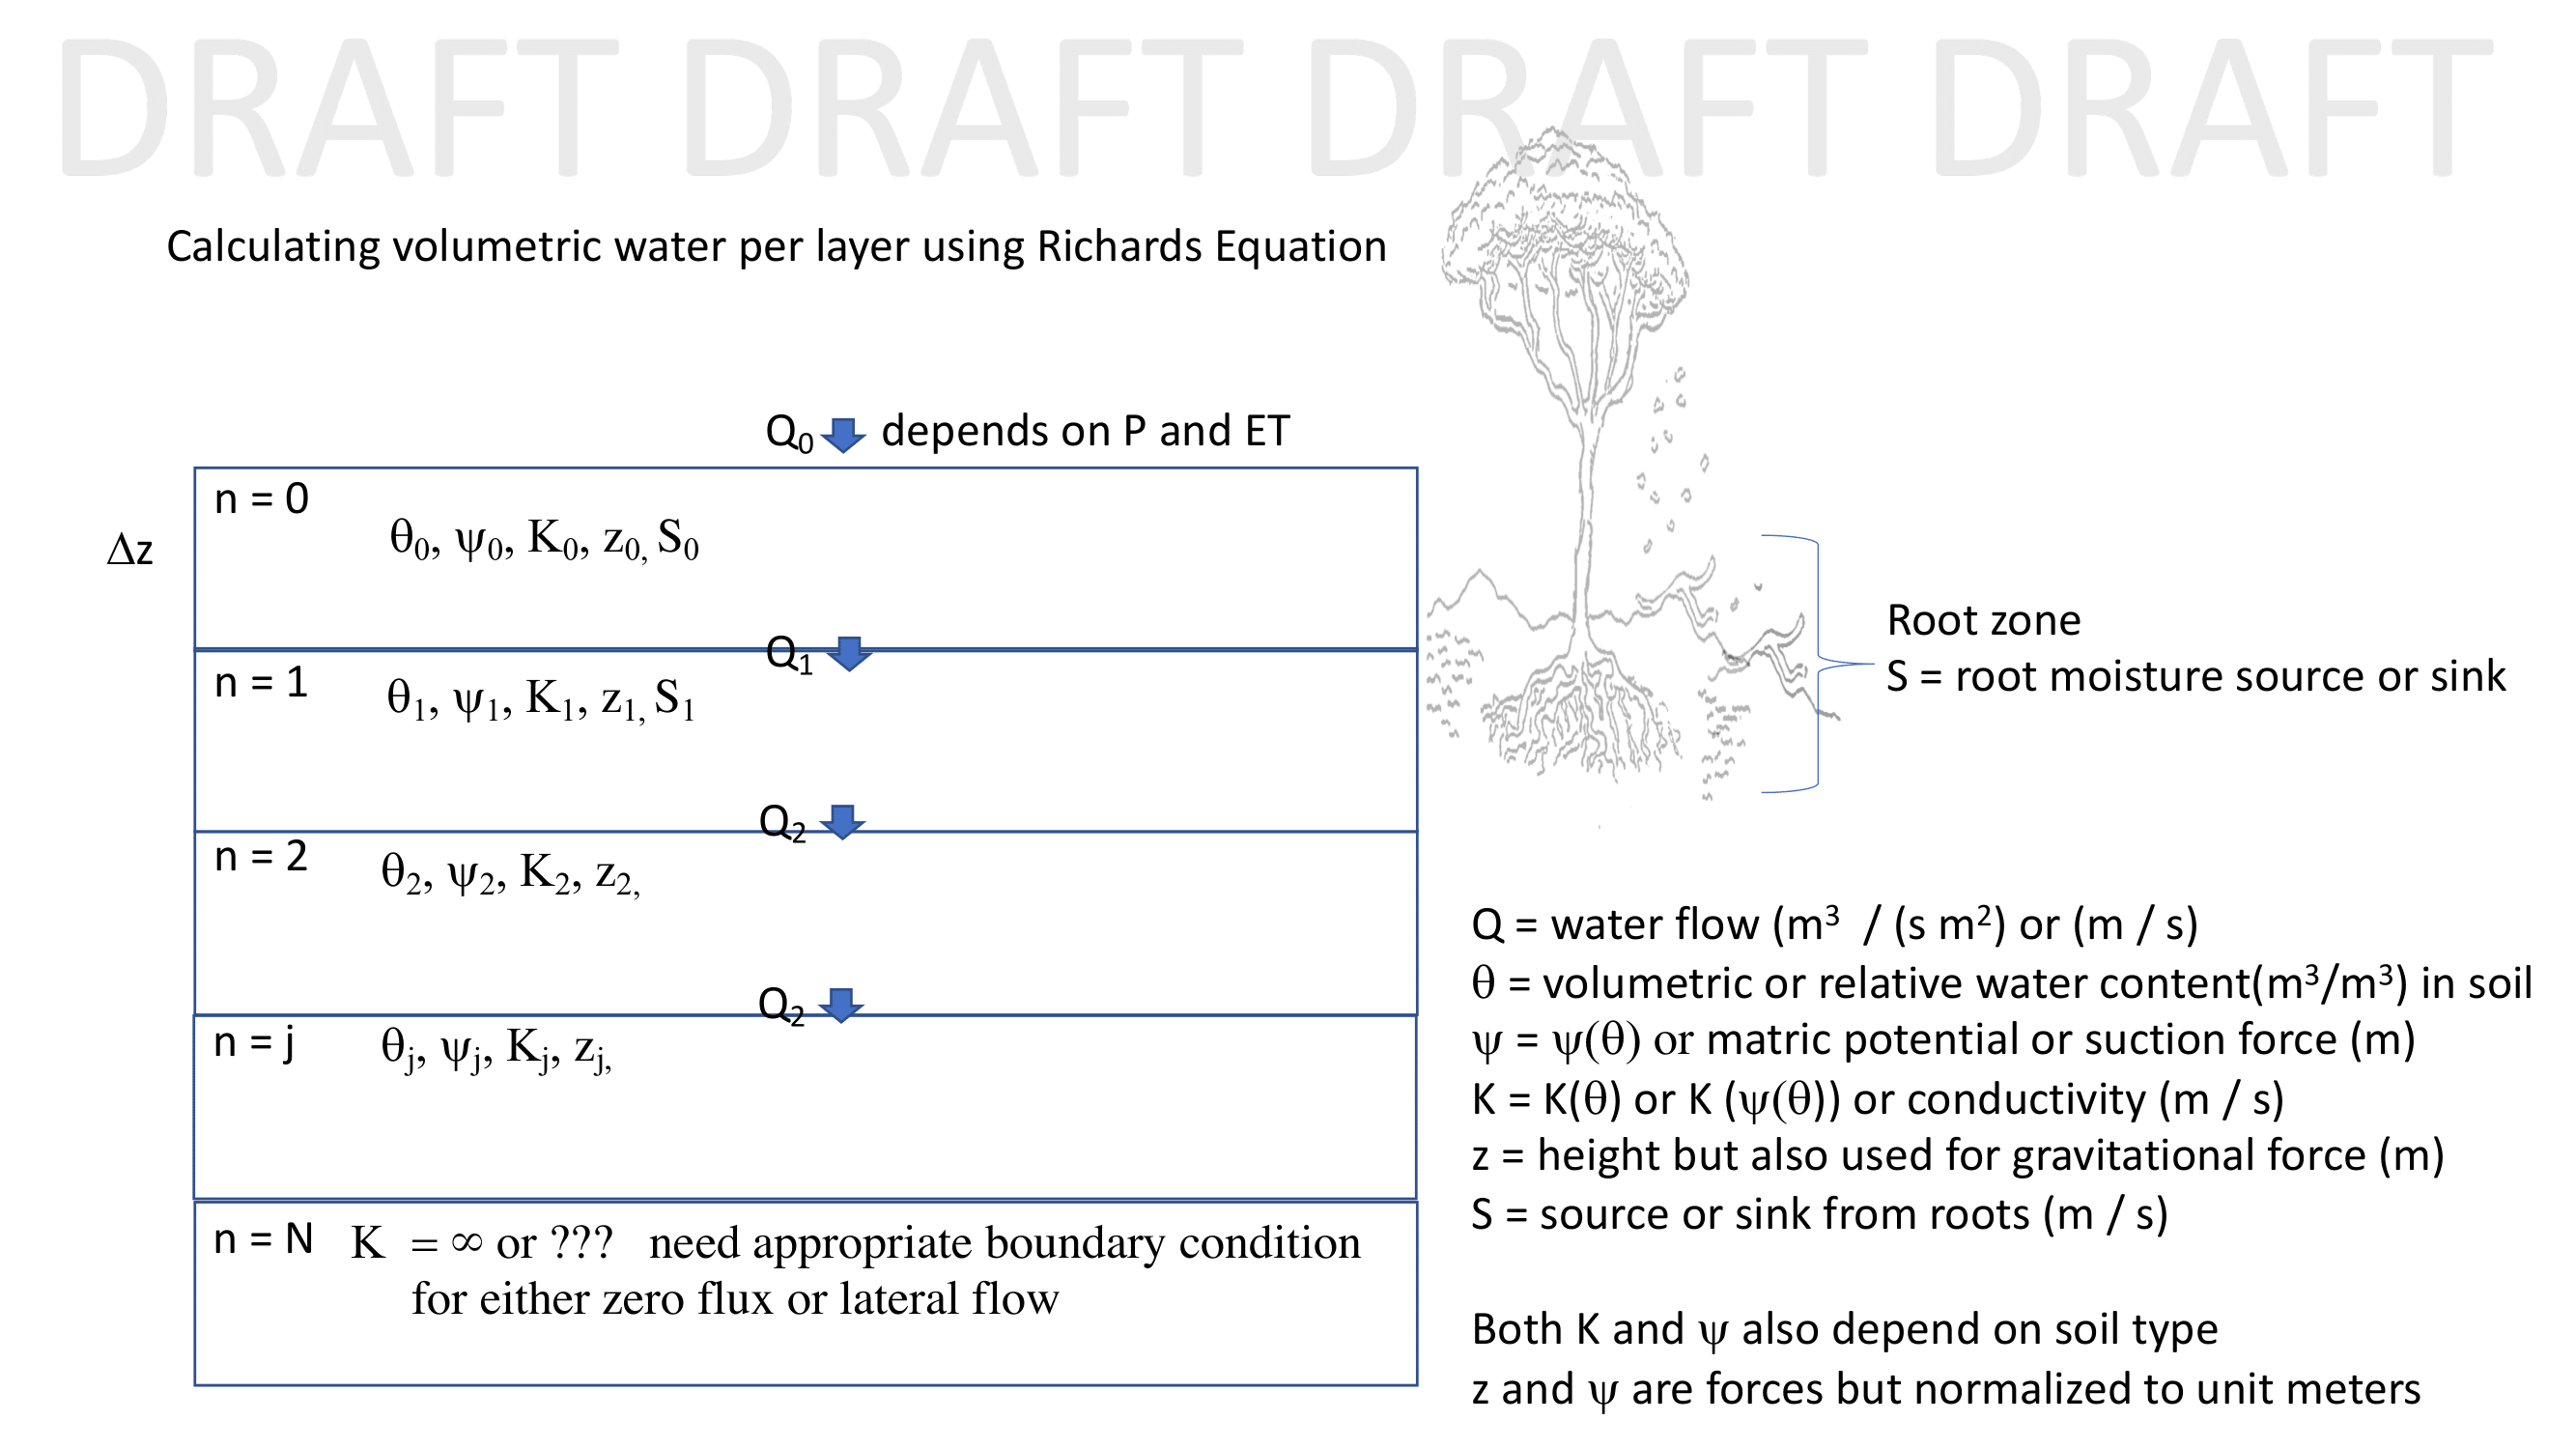
\includegraphics[scale=.15]{CLIMA-land/LM_figures/SoilSchematic-1.png}
\caption{Draft of soil schematic figure}
\end{figure}


\subsection{Phase Change}

The freezing of soil water or melting of soil ice releases or absorbs energy, respectively. Formation of ice releases latent heat, and temperature remains constant at the freezing point while soil water freezes. Similarly, melting of ice consumes energy, during which temperature does not increase. Latent heat of fusion is the amount of energy required to convert a unit of mass of frozen water to liquid. This transition requires 334 J g$^{-1}$. Freezing liquid water to ice releases a similar amount of energy. The total energy involved in phase change depends on soil moisture. For a volumetric water content $\theta$, the energy (J m$^{-3}$) required to freeze soil is $L_f \rho_{wat} \theta$, where $L_f =$ 0.334 MJ kg$^{-1}$ is the latent heat of fusion of water and $\rho_{wat} =$ 1000 kg m$^{-3}$ is the density of water. In course-grained soil such as sands, all the water present in the soil changes phase at a temperature close to 0$^{\circ}$C ($T_f =$ 273.15 K).  These soils can be treated with good approximation as either completely frozen or unfrozen. In fine-grain soils such as silts and clays, some soil water remains unfrozen even at temperatures below freezing. The amount of unfrozen water decreases as temperature decreases, and the latent heat release occurs over some temperature range $T_f - \Delta T_f$.

A simple way to account for freezing and thawing is to add the latent heat associated with phase change to the heat conduction equation to yield an apparent heat capacity \citep{lunardini1981heat}. Including a latent heat term as the unfrozen water $\theta_{liq}$ freezes, the heat conduction equation becomes
\begin{equation}
     c_v \frac{\partial T}{\partial t} = \frac{\partial }{\partial z} \left( \kappa \frac{\partial T}{\partial z} \right) - L_f \rho_{wat} \frac{\partial \theta_{liq}}{\partial t}.
\end{equation}
The second term on the right-hand side of the equation is a source of energy during freezing ($\partial \theta_{liq} / \partial t <$ 0) and is a sink of energy during melting ($\partial \theta_{liq} / \partial t >$ 0). The change in liquid water can be expressed as $\partial \theta_{liq} / \partial t = ( \partial \theta_{liq} / \partial T) (\partial T / \partial t)$, and the equation above can be re-written as 
\begin{equation}
     \left( c_v\ +\ L_f \rho_{wat} \frac{\partial \theta_{liq}}{\partial T} \right)  \frac{\partial T}{\partial t} = \frac{\partial }{\partial z} \left( \kappa \frac{\partial T}{\partial z} \right).
\end{equation}
Written this way, the term in parentheses on the left-hand side of the equation represents an effective heat capacity. Solution of this equation requires an expression for $\partial \theta_{liq}/{\partial T}$ to relate the amount of liquid water to temperature. In practice, however, the entire latent heat of fusion can be associated with a small finite temperature range between the freezing point and $T_f -\Delta T_f$ so that the effective heat capacity for a soil with water content $\theta$ is
\begin{equation}
c_v = \left\{
        \begin{array}{lll}
            c_{vu} & \quad T\ >\ T_f, \\
            c_{vf}\ + \frac{L_f \rho_{wat} \theta }{\Delta T_f} & \quad T_f - \Delta T_f\  \leq  T\ \leq\ T_f\ ,\\
            c_{vf} & \quad  T\ \leq\ T_f - \Delta T_f\\
        \end{array}
    \right.
\end{equation}
where $c_{vu}$ and $c_{vf}$ are the unfrozen and frozen volumetric heat capacity, respectively. The apparent heat capacity is the heat capacity of soil constituents plus a term that accounts for the latent heat of fusion. 

\begin{comment}

\hl{[The following is covered in Eq. (2.6) above.]} The heat capacity of air is negligible so that the heat capacity of soil is given by the weighted fraction of the heat capacity of solids, water and ice \citep{de1963thermal}, and
\begin{equation}
c_v = (1- \theta_{sat}) c_{v,sol} +  \theta_{liq} c_{v,wat} +  \theta_{i} c_{v,ice}.
\end{equation}
The heat capacity of water is $c_{v,wat}= \rho_{wat}c_{wat} =$ 4.19 MJ m$^{-3}$ K$^{-1}$, for ice $c_{v,ice}= \rho_{i}c_{i} =$ 1.94 MJ m$^{-3}$ K$^{-1}$, and for soil solids $c_{v,sol} =$ 1.926 MJ m$^{-3}$ K$^{-1}$ \citep{de1963thermal}. The equation above can be applied assuming all water is either liquid or ice to calculate the unfrozen and frozen heat capacity, respectively.  

\end{comment}

Using the chain rule of differentiation and the fact that the matric potential is a monotonic function of $\theta_l$, Darcy's law can also be written as
\begin{equation}\label{e:darcy_law2}
    \vec{\tilde d}_l = - K(\theta_l) \left(C_l(\theta_l)^{-1} \grad\theta_l + \grad \psi_z \right),
\end{equation}
where
\begin{equation}
C_l(\theta_l) = \left( \frac{d\psi}{d\theta_l} \right)^{-1} =   \frac{d\theta_l}{d\psi} 
\end{equation}
is known as the specific moisture capacity ($\mathrm{m^{-1}}$). The last equality is the derivative of the inverse $\theta_l(\psi)$ of the function $\psi(\theta_l)$, which is commonly used in hydrology and is known as the water retention curve. The quantity $K(\vec{\theta})/C(\vec{\theta})$ has units of diffusivity ($\mathrm{m^2~s^{-1}}$) is known as the soil water diffusivity. It is singular where the specific moisture capacity $C(\theta_l)$ is zero, which is the case in saturated soil. 

Integrating the water balance equation \eqref{e:soil_water_conservation} numerically is challenging primarily because of this singularity at the water table, where the unsaturated (vadose) zone meets the saturated zone \citep{Farthing17a}.

\subsection{Summary of soil heat and moisture equations for CliMA implementation}

This section contains a summary of all equations needed for implementation of the soil heat and moisture equations into CliMA. All variables are defined 

[OPTION: list equations in table for succinct description and avoid extra equation numbers in document] \\

\textbf{Soil Heat Equation} \\


\begin{equation}
     \frac{\partial (\rho_s c_s T_s) }{\partial t} = \frac{\partial }{\partial z}\kappa \frac{\partial T_s }{\partial z}
\end{equation}

\begin{equation}
    f_{\mathrm{om}} = \rho_{\mathrm{om}}/\rho_{om,{\rm max}}
\end{equation}


\begin{equation}
\kappa = K_e \kappa_{\rm sat} + (1-K_e) \kappa_{\mathrm{dry}}
\end{equation}

\begin{equation}
K_e = \exp \big( \gamma((1-s(\gamma-1.33))\big)
\end{equation}

\begin{equation}
s=\theta/\theta_{\rm sat}
\end{equation}

\begin{equation}
c_s=\theta c_{\rm liq} + (1-\theta) c_{\rm dry}
\end{equation}

\begin{equation}
c_{\rm dry} = (1-f_{\mathrm{om}})c_{soil} + f_{\mathrm{om}}c_{\mathrm{om}}
\end{equation}

\begin{equation}
c_{soil} = {\rm \frac{2.128 (sand)+ 2.385 (clay)}{(sand) + (clay)}}
\end{equation}  \\



\textbf{Soil Moisture Equations} \\

(Unsaturated soil)
\begin{equation}
 dS=d\theta 
\end{equation}

(Saturated - Unconfined Aquifer)
\begin{equation}
 dS=S_y dh ; S_y = n
\end{equation}

(Saturated - Confined Aquifer)
\begin{equation}
 dS=S_s dh
\end{equation}

\begin{equation}
 h=z+\psi
\end{equation}

\begin{equation}
dS = C(\psi)d\psi
\end{equation}

(Unsaturated soil)
\begin{equation}
C(\psi)=\partial \theta /\partial h 
\end{equation}

(Unconfined aquifer)
\begin{equation}
C(\psi)=S_y 
\end{equation}

(Richards' equation)
\begin{equation}
     \frac{\partial S}{\partial t} = C(\psi)\frac{\partial \psi}{\partial t} = -\divergence {\bf{q}} + {\rm Source}
\label{Richards}
\end{equation}

\begin{equation}
     \bf{q} = - \mathbf{K}(\psi) \otimes \nabla h
\end{equation}

(Unsaturated zone)
\begin{equation}
     \frac{\partial \theta}{\partial \psi}\frac{\partial h}{\partial t} = \frac{\partial}{\partial z} \left( {K(\psi)\frac{\partial \psi}{\partial z}} + 1 \right) + {\rm Source}
\end{equation} \\

(Saturated - Unconfined Aquifer)
\begin{equation}
     \frac{\partial S}{\partial t} = S_y \frac{\partial h}{\partial t} = \divergence \left( {K_{\rm sat} \nabla h} \right) + {\rm Source}
\end{equation} \\


\textbf{Retention functions for unsaturated soils - van Genuchten} \\


\begin{equation}
     \theta(\psi) = \theta_{\mathrm{res}} + \frac{\theta_{\mathrm{sat}} - \theta_{\mathrm{res}}}{\left[ 1+(\alpha |\psi|)^n \right]^{m}}
\end{equation}

\begin{equation}
m=1-1/n
\end{equation}

\begin{equation}
     K(\psi) = K_{\mathrm{sat}} S_l^L \left (1 -  (1-S_l^{1/m})^m  \right)^2
\end{equation}

\begin{equation}
L = 0.5
\end{equation}

\begin{equation}
     S_l = \frac{\theta(\psi) - \theta_{\mathrm{res}}}{\theta_{\mathrm{sat}} - \theta_{\mathrm{res}}}
\end{equation}

\begin{equation}
     \frac{\partial \theta}{\partial \psi} =   \frac{m n\alpha^n |\psi|^{n-1}}{\left[ 1+(\alpha |\psi|)^n \right]^{m+1}} \left( \theta_{\mathrm{sat}} - \theta_{\mathrm{res}} \right) 
\end{equation}


\subsubsection{Retention curves $\theta=f(\psi)$ and $K(\psi)$ in the unsaturated zone}
\label{SoilMoisture:Retention_Curves}
    {\bf Van Genuchten} \\
We will use the van Genuchten formulation as a reference retenstion curve, as it is better behaved in saturated conditions than the Brooks and Corey relationship 
\begin{equation}
     \theta(\psi) = \theta_{\mathrm{res}} + \frac{\theta_{\mathrm{sat}} - \theta_{\mathrm{res}}}{\left[ 1+(\alpha |\psi|)^n \right]^{m}}
\end{equation}
with $m=1-1/n$.
For hydraulic conductivity, we have
\begin{equation}
     K(\psi) = K_{\mathrm{sat}} S_l^L \left (1 -  (1-S_l^{1/m})^m  \right)^2
\end{equation}
with $L$ an empirical parameter assumed to be $L=0.5$. $S_l$ is the relative degree of saturation of the soil and $K_{\mathrm{sat}}$ the hydraulic conductivity at saturation. 
\begin{equation}
     S_l = \frac{\theta(\psi) - \theta_{\mathrm{res}}}{\theta_{\mathrm{sat}} - \theta_{\mathrm{res}}}
\end{equation}
The derivative of $\theta$ with respect to $\psi$, $C(\psi)$ is:
\begin{equation}
     \frac{\partial \theta}{\partial \psi} =   \frac{m n\alpha^n |\psi|^{n-1}}{\left[ 1+(\alpha |\psi|)^n \right]^{m+1}} \left( \theta_{\mathrm{sat}} - \theta_{\mathrm{res}} \right). 
\end{equation}


    {\bf Brooks and Corey} \\
An alternative approach to Van Genuchten will be to use the Brooks-Corey relationships:
\begin{equation}
     \theta(\psi) = \theta_{\mathrm{res}} + (\theta_{\mathrm{sat}} - \theta_{\mathrm{res}})\left( \frac{\psi}{\psi_{ae}}\right)^{-\lambda}
\end{equation}
with $\psi_{ae}$ the air entry point.
\begin{equation}
     K(\psi) = K_{\mathrm{sat}} \left( \frac{\psi}{\psi_{ae}}\right)^{-2-3\lambda}
\end{equation}


% Calculation of Kersten number and kappa_s for Thermal Conductivity calculation 
\begin{comment}
For unfrozen soil: \hl{[what is this based on? does it have a strong basis in global data?]}
\begin{equation}
K_e = \left\{
        \begin{array}{ll}
            1.0 + 0.7\ \mathrm{log_{10}}\ S_l & \mathrm{course-texture\ soil\ } (S_l > 0.05), \\
            1.0 + \mathrm{log_{10}}\ S_l & \mathrm{fine-texture\ soil\ } (S_l > 0.10)
        \end{array}
    \right.
\end{equation}
and fine-texture soil has a sand content of less than 50\%. For frozen soil:
\begin{equation}
K_e = S_l.
\end{equation}
In these equations, $S_l= \frac{\theta}{\nu_p}$ is the relative wetness, with $\theta$ as the volumetric water content (m$^{3}$ H20 m$^{-3}$ soil) and $\nu_p=\theta_{sat}$ as the volumetric water content at saturation (also equal to porosity). 

The dry and saturated thermal conductivities depend on soil properties. The thermal conductivity of dry soils varies with bulk density (kg m$^{-3}$) according to 
\begin{equation}
\kappa_{\mathrm{dry}} = \frac{ (0.135 \rho_\mathrm{b} + 64.7 )}{ (2700 - 0.947 \rho_\mathrm{b} )}.
\end{equation}
where $\rho_\mathrm{b} = 2700(1- \theta_{sat})$ and 2700 kg m$^{-3}$ here represents the density of soil solids. The thermal conductivity of saturated soil is calculated from the thermal conductivity of the components (solids $\kappa_{solids}$, water $\kappa_{liquid}$, and ice $\kappa_{i}$) and their respective volume fractions. For unfrozen soil:
\begin{equation}\label{e:conductivity_sat}
\kappa_{\mathrm{sat}} = \kappa_{solids}^{(1- \theta_{sat} )}  \kappa_{liquid}^{(\theta_{sat} )}. 
\end{equation}
And for frozen soil:
\begin{equation}
\kappa_{\mathrm{sat}} = \kappa_{solids}^{(1- \theta_{sat} )}  \kappa_{i}^{(\theta_{sat} )}. 
\end{equation}
A general expression allowing a mixture of liquid water and ice is
\begin{equation}
\kappa_{\mathrm{sat}} = \kappa_{solids}^{(1- \theta_{sat} )}  \kappa_{liquid}^{(f_u \theta_{sat} )}  \kappa_{i}^{( (1-f_u) \theta_{sat} )}.
\end{equation}
This equation recognizes that even at temperatures below freezing, the total water consists of unfrozen $\theta_{liq}$ and frozen $\theta_{i}$ water ($\theta = \theta_{liq} + \theta_{liq}$), and $f_u = \frac{\theta_{liq}}{\theta}$ is the fraction of the total water that is unfrozen. Representative values are $\kappa_{liquid} = 0.57$ W m$^{-1}$ K$^{-1}$ and $\kappa_{i} = 2.29$ W m$^{-1}$ K$^{-1}$. 
The thermal conductivity of a soil varies with the quartz content of the soil. The Johansen method described by \citep{Farouki81a} gives an approximation of such a dependence on quartz content:
\begin{equation}
\kappa_{solids} = \kappa_{q}^q \kappa_{o}^{1-q},
\end{equation}
where $q$ is the quartz content as a fraction of the total soil solids, $\kappa_{q}$ = 7.7 W m$^{-1}$ K$^{-1}$ is the thermal conductivity of quartz, and $\kappa_{o}$ = 2.0 W m$^{-1}$ K$^{-1}$ is the thermal conductivity of other minerals for soils with $q >$ 0.2 and  $\kappa_{o}$ = 3.0 W m$^{-1}$ K$^{-1}$ for $q <=$ 0.2. The accuracy of this equation depends on the specified thermal conductivity of quartz and the quartz fraction. The quartz content can be approximated by the sand content (i.e. quartz fraction $q$ $\sim$= fraction of soil that is sand)  \citep{peters1998effect}, though this is not necessarily correct \citep{lu2007improved}.  
\end{comment}


% Old Explanation of Calculation of Kersten number and kappa_s for Thermal Conductivity calculation
\begin{comment}
The thermal conductivity of soil depends on the water content and is modeled as a weighted mean of a conductivity $\kappa_{\mathrm{dry}}$ of dry soil and a conductivity $\kappa_{\rm sat}$ of water-saturated soil,
\begin{equation}\label{e:soil_conductivity}
\kappa = K_e \kappa_{\mathrm{sat}} + (1-K_e) \kappa_{\mathrm{dry}}.
\end{equation}
The weighting factor $K_e$ is the Kersten number, which is function of soil relative humidity $s=\theta/\theta_{\rm sat}$. (However, the thermal diffusivity $\kappa/\tilde c_s$ has a much weaker moisture dependence than $\kappa$ itself because of a compensation of the moisture dependence between $\kappa$ and $\tilde c_s$.)

The saturation heat conductivity, even in the presence of frozen ground, can be expressed as a function of the ice and liquid water contents assuming a geometric mean: \hl{[why do we average geometrically here and arithmetically above? Seems odd.]}
\begin{equation}\label{e:conductivity_sat}
\kappa_{\mathrm{sat}} = \kappa_{solids}^{(1- \theta_{sat} )}  \kappa_{liquid}^{(f_u \theta_{sat} )}  \kappa_{i}^{( (1-f_u) \theta_{sat} )} 
\end{equation}
where $\kappa_{\mathrm{sat}}$ is the thermal conductivity of a saturated soil, and is calculated from the thermal conductivity of the components ($\kappa_{solids}$, $\kappa_{liquid}$, and $\kappa_{i}$), $\theta_{sat}$ is the volumetric water content at saturation (also equal to porosity), and $f_u = \theta_{liquid} / \theta$ is the fraction of total water that is unfrozen. Representative values are $\kappa_{liquid} = 0.57$ W m$^{-1}$ K$^{-1}$ and $\kappa_{i} = 2.29$ W m$^{-1}$ K$^{-1}$. 
The thermal conductivity of a soil varies with the quartz content of the soil. The Johansen method described by \cite{Farouki81a} gives an approximation of such a dependence on quartz content:
\begin{equation}
\kappa_{solids} = \kappa_{q}^q \kappa_{o}^{1-q}
\end{equation},
where $q$ is the quartz content as a fraction of the total soil solids, $\kappa_{q}$ = 7.7 W m$^{-1}$ K$^{-1}$ is the thermal conductivity of quartz, and $\kappa_{o}$ = 2.0 W m$^{-1}$ K$^{-1}$ is the thermal conductivity of other minerals for soils with $q >$ 0.2 and  $\kappa_{o}$ = 3.0 W m$^{-1}$ K$^{-1}$ for $q <=$ 0.2.
\end{comment}


\subsection{Moisture equation - an alternative approach}

We note that there is a fundamental issue in the continuity of the Richards' equation at the water table interface. Indeed, $C(\psi)$ goes to zero at the bottom of the unsaturated zone but is a fixed value in the saturated zone (the specific yield), leading to sharp derivative discontinuity. We note that the specific yield is empirical, mainly based on measurements and is close to the soil moisture content at saturation $\theta_{\mathrm{sat}}$. We will return to this.

We write the porous medium temporal mass $M$ balance per unit volume as a departure from the hydrostatic pressure, equivalent to $\partial h/\partial z=0$, with $h=z+\psi$. The temporal departure from hydrostatic balance is written as $\psi'$ with corresponding changes in density $\rho'=\rho-\overline\rho$. The water porous medium density conservation reads:
\begin{equation}
\frac{\partial \rho \theta}{\partial t} = {\overline{\rho}} \divergence \left( K(\psi) \left( \nabla \psi + {\mathbf e_z} \right) \right)
\end{equation}
In which we have neglected the mass of water vapor.
We expand this into:
\begin{equation}
{\overline \rho} \frac{\partial \theta}{\partial t} + \theta \frac{\partial \rho}{\partial t} = {\overline \rho} \divergence \left( K(\psi) \left( \nabla \psi + {\mathbf e_z} \right) \right)
\end{equation}
Dividing by $\overline \rho$ gives:
\begin{equation}
\frac{\partial \theta}{\partial t} + \frac{\theta}{\overline \rho} \frac{\partial \rho}{\partial t} = \divergence \left( K(\psi) \left( \nabla \psi + {\mathbf e_z} \right) \right)
\end{equation}
This equation looks like the unsaturated Richards’ equation beside the presence of the second term on the left hand side, related to the compressibility of liquid water: $ \frac{\theta}{\overline \rho} \frac{\partial \rho}{\partial t}$.

We now use chain’s rule with respect to variations in internal pressure $\psi$ but do not assume that liquid water is incompressible, to write the mass change:
\begin{equation}
{\overline \rho} \frac{\partial \theta}{\partial t} + \theta \frac{\partial \rho}{\partial t} 
\end{equation}

In the unsaturated zone the second term on the lhs is negligible. In the saturated zone, the converse is true and the density term becomes important. At the water table interface, the $\theta=\theta_{\mathrm{sat}}=n$, the porosity assumed to be the same as the saturation water content $\theta_{s}$. We therefore further write $\theta$ in terms of the relative saturation content $s=\theta/\theta_{\mathrm{sat}}$.
The liquid water mass balance can be written
\begin{equation}
\underbrace{{\overline \rho} n \frac{\partial s}{\partial t} }_\text{\rm unsaturated mass change} + \underbrace{{\overline \rho} s \frac{\partial n}{\partial t}  }_\text{\rm change in porous medium porosity}  
+ 
\underbrace{\theta \frac{\partial \rho}{\partial t}   }_\text{\rm change in liquid water density}  
\label{mass_balance:split}
\end{equation}
The change in density (assuming negligible temperature and solute impact) can be written:
\begin{equation}
\frac{\partial \rho}{\partial t} = \rho \beta \frac{\partial \psi}{\partial t}
\end{equation}
with $\psi$ the pressure.
Assumed an elastic material (and neglecting the change in density of the material) (Bear 2018) and introducing the coefficient of porous medium compressibility $\alpha_{pm}$, with assumed veritcal stress:
\begin{equation}
\alpha_{pm}=\frac{1}{V_{pm}} \frac{\partial V_{pm}}{\partial \sigma_z} = \frac{1}{1-n} \frac{\partial n}{\partial \psi}
\end{equation}
with $\sigma_z$ the stress tensor in the vertical direction.
This then lead to the change in porosity due to the porous medium compaction:
\begin{equation}
\frac{\partial n}{\partial t} = (1-n)\alpha_{pm}\frac{\partial \psi}{ \partial \psi}
\end{equation}
The combined change in mass of the porous medium water can be finally written using equation (\ref{mass_balance:split}) 
\begin{equation}
\frac{\partial \theta \rho}{\partial t} = 
\underbrace{n \rho \frac{\partial s}{ \partial t} }_\text{\rm unsaturated mass change} + \underbrace{s \rho \left[  (1-n)\alpha_{pm} + n\beta \right] \frac{\partial \psi}{\partial t} }_\text{\rm saturated mass change}
\end{equation}
We note here that we made a convenient approximation: we used the matric potential $\psi$, instead of the pressure $p$. The rational for that is that far away from the water table the unsaturated term the left hand side domaintes. Within the saturated zone, far from the water table, the lhs vanishes. Yet an advantage is that the equation bcomes continuous at the interface, with continuous and non-vanishing temporal derivatives. Another way to think about this is that the fluid is composed of a mixture of saturated and saturated water at the interface - i.e the interface is not abrupt. 
Our master equation for the porous medium water conservation then becomes:
\begin{equation}
 \left( n \rho \frac{\partial s}{\partial \psi} + s \rho   (1-n)\alpha_{pm} + s n\beta \right) \frac{\partial \psi}{\partial t} = \rho \divergence \left( K(\psi) \left( \nabla \psi + {\mathbf e_z} \right) \right)
\label{master_equation_porous_medium}
\end{equation}
or dividing by $\rho$
\begin{equation}
\red{ n \left(  \frac{\partial s}{\partial \psi} + s \frac{1-n}{n}\alpha_{pm} + s \beta \right) \frac{\partial \psi}{\partial t} = \divergence \left( K(\psi) \left( \nabla \psi + {\mathbf e_z} \right) \right)}
\label{master_equation_porous_medium} 
\end{equation}







We now integrate the mass balance equation over the depth of the unconfined aquifer i.e. from $z=z_0$ to $z=h+\epsilon$ (with $z=z_0$ the bedrock elevation – not necessarily 0):
\begin{equation}
\int_{z_0}^{h+\epsilon} { n \left(  \frac{\partial s}{\partial \psi} + s \frac{1-n}{n}\alpha_{pm} + s \beta \right) \frac{\partial \psi}{\partial t}  dz = \int_{z_0}^{h+\epsilon} \divergence \left( K(\psi) \left( \nabla \psi + {\mathbf e_z} \right) \right)} dz
\end{equation}
\begin{equation}
\int_{z_0}^{h+\epsilon} { n \left(  \frac{\partial s}{\partial \psi} + s \frac{1-n}{n}\alpha_{pm} + s \beta \right) \frac{\partial \psi}{\partial t}  dz =
K(\psi) \left( \frac{\partial \psi}{\partial z} + 1 \right)_{|z=h+\epsilon} + \nabla_H \cdot \int_{z_0}^{h+\epsilon}  K(\psi) \nabla_H \psi dz
\end{equation}
Using Leibniz rule, the lhs can be written as 
\begin{equation}
\frac{\partial \int_{z_0}^h \rho \theta_{\mathrm{sat}} dz }{\partial t} - \rho \theta_{\mathrm{sat}} \frac{\partial h}{\partial t}=
K(\psi) \left( \frac{\partial \psi}{\partial z} + 1 \right)_{|z=h+\epsilon} \\
+ \nabla_H \cdot \int_{z_0}^{h+\epsilon}  K(\psi) \nabla_H \psi dz
\end{equation}
The rhs can be rewritten as:
\begin{equation}
\int_{z_0}^h  \divergence \left( {\overline \rho} K(\psi) \left(\nabla \psi + {\mathbf e_z} \right) \right) dz = {\overline \rho} K(\psi) \left(\nabla \psi + {\mathbf e_z} \right)_{|h}  + \int_{z_0}^h  \nabla_H \left( {\overline \rho} K(\psi) \left(\nabla_H \psi \right) \right) dz
\end{equation}

Because the rate of change of the water table is much larger than the changes in density, we have: 
\begin{equation}
-	\theta_{\mathrm{sat}} \frac{\partial h}{\partial t} = 
 K(\psi) \left(\nabla \psi + {\mathbf e_z} \right)_{|h}  + \int_{z_0}^h  \nabla_H \left( {\overline \rho} K(\psi) \left(\nabla_H \psi \right) \right) dz
\end{equation}

Using the total derivative of $\theta$, we can write:

\section{Older Stuff}

\hl{[TS: I'd like to keep things simple for now, mostly confined to what is above, to see how far we get with it. Some things here are clearly more complex than we need (e.g., I don't think we want to introduce compressibility of soil water here. This would introduce a host of complications, including an inability to use volume fractions etc. --- I also strongly prefer conservation laws (such as (2.18)) over formulations like some below that, when discretized, do not guarantee conservation of water and energy.]}

Moisture conservation is usually divided into two regions: 1) the unsaturated zone where total water storage is related to the relative water content $\theta$ and transport is typically assumed to be 1D in the vertical and 2) the saturated zone where water storage is related to changes in the water head through the storativity or specific yield, and which is treated as a bulk average over the aquifer thickness. Ice water will be assumed to only originate from local phase changes but not advected around. 
Let us start with the 3D Richards' equation so we do not lose generality (1D flow is just an approximation similar to shallow water equation). Water storage is written as $S$ (units of $m^3/m^3$). For instance in the unsaturated soil, the storage is related to the water content $S=\theta$. In an unconfined aquifer $dS=S_y dh$, with $S_y$ the unconfined aquifer specific yield, nearly equal to porosity $n$. Finally, in the confined aquifer $dS=S_s dh$, with $S_s$ the aquifer storativity. Note that the concept of aquifer storativity implicitly assumes a vertically-integrated Richards' equation over the thickness of the aquifer $b$. 

Without loss of generality we can therefore write the storage as a (nonlinear) function of the head 
\begin{equation}
     h=z+\psi,
\label{head}
\end{equation}

with $\psi$ the matric potential so that $dS = C(\psi)d\psi$. In the unsaturated case C($\psi$)=$\partial \theta /\partial h$ \\ and in the saturated (unconfined aquifer) case it is the specific yield $C(\psi)=S_y$.
We therefore write the conservation of mass including sinks/sources (such as due to roots but also for instance non-local transport due to preferential flow). 
So the generic 3D Richards' equation using chain's rule:
\begin{equation}
     \frac{\partial S}{\partial t} = C(\psi)\frac{\partial \psi}{\partial t} = -\divergence {\bf{q}} + S_q
\label{Richards}
\end{equation}
with $S_l$ a source of liquid water, including the ice to liquid water melting process and the extraction of water by transpiration.
$\bf{q}$ is Darcy's flow, with 
\begin{equation}
     \bf{q} = - \mathbf{K}(\psi) \otimes \nabla h
\end{equation} with $ \mathbf{K}$ the hydraulic conductivity tensor, and $\otimes$ the tensor product.
For simplicity we will assume that the flow is isotropic and therefore along the head gradient (this might not be true because of the strong horizontal layering of the soil creating important anisotropy; this could be relaxed later):
\begin{equation}
     {\bf{q}} = - K \ \nabla h
\end{equation}
So we are left with our simplified Richards' 3D equation:
\begin{equation}
     C(\psi)\frac{\partial \psi}{\partial t}  = \divergence \left( {K(\psi) \nabla h} \right) + S_q
\label{Richards_simple}
\end{equation}
Equation (\ref{Richards_simple}) written in head term is continuous across saturation interfaces.
We finally write this in terms of $\psi$ only
\begin{equation}
     C(\psi)\frac{\partial \psi}{\partial t}  = \divergence \left( K \left( \nabla \psi + {\mathbf e_z} \right) \right) + S_q
\label{Richards_simple_bis}
\end{equation}

{\bf Unsaturated zone}\\
In the unsaturated zone, the storage is simply $S=\theta$, so that $C=d\theta/d\psi$, which is the so-called retention curves (assuming negligible hysteresis). The potential options for the retention curves are discussed in section \ref{SoilMoisture:Retention_Curves}. We keep a head-based approach for Richard's equation, for continuity.
\begin{equation}
     \frac{\partial \theta}{\partial \psi}\frac{\partial \psi}{\partial t}  = \divergence \left( K \left( \nabla \psi + {\mathbf e_z} \right) \right) + S_q
\label{Richards_simple_unsaturated}
\end{equation}
Assuming that the flow is mostly 1D in the vertical this further simplifies to:
\begin{equation}
     \frac{\partial \theta}{\partial \psi}\frac{\partial h}{\partial t} = \frac{\partial}{\partial z} \left( {K(\psi)\frac{\partial \psi}{\partial z}} + 1 \right) + S_q
\label{Richards_simple_uns_1D}
\end{equation}
We note however that as the horizontal resolution becomes finer and in the presence of rain this 1D assumption is not tenable anymore

{\bf Unconfined aquifer}\\
In an unconfined aquifer, below the water table, we will use a bulk average equation integrated over the depth of the aquifer, and the storage over the entire depth is written as a function of the specific yield $S_y$. Therefore we integrate equation \ref{Richards_simple_bis} over the depth $h$ of the aquifer.
\begin{equation}
     \frac{\partial S}{\partial t} = S_y \frac{\partial h}{\partial t}  + \overline{S_q}
\end{equation}
this will lead to the following equation:
\begin{equation}
     \frac{\partial S}{\partial t} = S_y \frac{\partial h}{\partial t} = \divergence \left( {K_{\rm sat} \nabla h} \right) + \overline{S_q}
\label{Richards_simple}
\end{equation}
with $K_{\rm sat}$ the saturated hydraulic conductivity. 

{\bf Correction of hydraulic conductivity in the presence of ice water}\\
Ice water modifies the hydraulic conductivity of water because it changes the tortuosity of the porous medium. In that case the hydraulic conductivity $K$ becomes $K \Theta_{i}$, with $\Theta_{i}$ an empirical correction factor dependent on the fraction of ice water. An example of scuh an empirical facotr was developed by Swenson et al. 2012, $\Theta_{i}=10^{-\Omega f_{i}}$, with $\Omega=6$ and $f_{i}=\theta_{ice}/\theta_{sat}$.







